% ============================================================
%  يُترجَم بـ XeLaTeX  (في Overleaf: Menu → Compiler → XeLaTeX)
%  الخط: Amiri (متوفر في Overleaf، أو حمّله من github.com/aliftype/amiri)
% ============================================================
\documentclass[12pt,a4paper]{article}
\usepackage[a4paper,margin=1.7cm,top=2.3cm,bottom=2.9cm,headheight=15pt,footskip=1.5cm]{geometry}
\usepackage{amsmath,amssymb}
\usepackage{icomma}
\usepackage[english,bidi=default,layout=lists]{babel}
\babelprovide[import,main]{arabic}
\babelfont{rm}[Scale=1.08]{Amiri}
\babelfont{sf}[Scale=1.08]{Amiri}
\usepackage[most]{tcolorbox}
\usepackage{tikz}
\usetikzlibrary{arrows.meta,calc,shadings}
\usepackage{array}
\usepackage{colortbl}
\usepackage{fancyhdr}
\usepackage{titlesec}
\usepackage{enumitem}
\usepackage{collcell}
\usepackage{needspace}
\usepackage{etoolbox}
\newcolumntype{C}{>{\collectcell\ar}c<{\endcollectcell}}
\pretocmd{\section}{\Needspace{15\baselineskip}}{}{}
\pretocmd{\subsection}{\Needspace{11\baselineskip}}{}{}

\definecolor{cDef}{HTML}{1F4E9C}
\definecolor{cThm}{HTML}{B3261E}
\definecolor{cRem}{HTML}{2E7D32}
\definecolor{cEx}{HTML}{C76B00}
\definecolor{cMeth}{HTML}{6A1B9A}
\definecolor{cSol}{HTML}{00695C}
\definecolor{cSec}{HTML}{1F3A68}

\titleformat{\section}{\Large\bfseries\color{cSec}}{\thesection.}{0.6em}{}[{\color{cSec!60}\titlerule[1pt]}]
\titleformat{\subsection}{\large\bfseries\color{cThm!85!black}}{\thesubsection.}{0.5em}{}
\titlespacing*{\section}{0pt}{14pt}{8pt}
\titlespacing*{\subsection}{0pt}{10pt}{5pt}
\setlength{\parindent}{0pt}
\setlength{\parskip}{4pt}
\setlist{itemsep=2pt,topsep=3pt}

\newtcolorbox{arbox}[3][]{enhanced,
  colback=#2!5,colframe=#2!80!black,arc=2mm,boxrule=0.8pt,
  left=6pt,right=6pt,top=8pt,bottom=5pt,
  fonttitle=\bfseries,coltitle=white,
  title={\foreignlanguage{arabic}{#3}},
  attach boxed title to top right={xshift=-5mm,yshift=-3mm},
  boxed title style={colback=#2!80!black,arc=1.5mm,boxrule=0pt},
  before upper={\selectlanguage{arabic}},
  before skip=8pt,after skip=8pt,breakable,#1}
\newenvironment{BOX}[2]{\begin{otherlanguage}{english}\begin{arbox}{#1}{#2}}{\end{arbox}\end{otherlanguage}}
\newenvironment{tarif}[1][تعريف]{\begin{BOX}{cDef}{#1}}{\end{BOX}}
\newenvironment{khassia}[1][خاصية]{\begin{BOX}{cThm}{#1}}{\end{BOX}}
\newenvironment{molahada}[1][ملاحظة]{\begin{BOX}{cRem}{#1}}{\end{BOX}}
\newenvironment{mithal}[1][مثال]{\begin{BOX}{cEx}{#1}}{\end{BOX}}
\newenvironment{tariqa}[1][طريقة]{\begin{BOX}{cMeth}{#1}}{\end{BOX}}

\newcounter{exo}
\newenvironment{tamrin}[1]{\stepcounter{exo}\begin{BOX}{cSec}{التمرين \theexo: #1}}{\end{BOX}}
\newenvironment{hal}{\Needspace{12\baselineskip}\begin{otherlanguage}{english}\begin{arbox}[breakable]{cSol}{حل التمرين \theexo}}{\end{arbox}\end{otherlanguage}}

\newenvironment{LTR}{\begin{otherlanguage}{english}}{\end{otherlanguage}}
\newcommand{\ar}[1]{\foreignlanguage{arabic}{#1}}

\renewcommand{\dots}{\mathinner{\ldotp\ldotp\ldotp}}
\renewcommand{\ldots}{\mathinner{\ldotp\ldotp\ldotp}}
\renewcommand{\cdots}{\mathinner{\cdotp\cdotp\cdotp}}
\newcommand{\N}{\mathbb{N}}
\newcommand{\Z}{\mathbb{Z}}
\newcommand{\D}{\mathbb{D}}
\newcommand{\Q}{\mathbb{Q}}
\newcommand{\R}{\mathbb{R}}
\newcommand{\pgcd}{\operatorname{PGCD}}
\newcommand{\ppcm}{\operatorname{PPCM}}

% \NLseg{a}{b}{[}{]} ; \NLright{a}{[} ; \NLleft{b}{]}  (interval on a number line)
\newcommand{\NLseg}[4]{\begin{LTR}\begin{tikzpicture}[baseline=-0.6ex]
 \draw[-{Stealth[length=2mm]},gray!70](0,0)--(3.4,0);
 \draw[line width=2pt,cThm!80!black](0.7,0)--(2.7,0);
 \node[cThm!80!black,font=\LARGE] at (0.7,0){$#3$};
 \node[cThm!80!black,font=\LARGE] at (2.7,0){$#4$};
 \node[below=3pt,font=\footnotesize] at (0.7,0){$#1$};
 \node[below=3pt,font=\footnotesize] at (2.7,0){$#2$};
\end{tikzpicture}\end{LTR}}
\newcommand{\NLright}[2]{\begin{LTR}\begin{tikzpicture}[baseline=-0.6ex]
 \draw[-{Stealth[length=2mm]},gray!70](0,0)--(3.4,0);
 \draw[line width=2pt,cThm!80!black](1.3,0)--(3.3,0);
 \node[cThm!80!black,font=\LARGE] at (1.3,0){$#2$};
 \node[below=3pt,font=\footnotesize] at (1.3,0){$#1$};
\end{tikzpicture}\end{LTR}}
\newcommand{\NLleft}[2]{\begin{LTR}\begin{tikzpicture}[baseline=-0.6ex]
 \draw[-{Stealth[length=2mm]},gray!70](0,0)--(3.4,0);
 \draw[line width=2pt,cThm!80!black](0.05,0)--(2.1,0);
 \node[cThm!80!black,font=\LARGE] at (2.1,0){$#2$};
 \node[below=3pt,font=\footnotesize] at (2.1,0){$#1$};
\end{tikzpicture}\end{LTR}}

% ---------- social-media icons (pure TikZ) ----------
\definecolor{cFB}{HTML}{1877F2}
\definecolor{cTG}{HTML}{229ED9}
\definecolor{cIG1}{HTML}{FEDA75}
\definecolor{cIG2}{HTML}{D62976}
\definecolor{cIG3}{HTML}{4F5BD5}
\newcommand{\fbicon}{\begin{LTR}\begin{tikzpicture}[baseline=-0.75ex,x=1em,y=1em]
 \fill[cFB] (0,0) circle (0.55);
 \node[white,inner sep=0,font=\usefont{TU}{lmss}{bx}{n}\small] at (0.04,-0.02) {f};
\end{tikzpicture}\end{LTR}}
\newcommand{\igicon}{\begin{LTR}
\begin{tikzpicture}[baseline=-0.75ex,x=1em,y=1em]
 \shade[lower left=cIG1,lower right=cIG2,upper left=cIG2,upper right=cIG3,rounded corners=0.28em] (-0.55,-0.55) rectangle (0.55,0.55);
 \draw[white,line width=0.09em,rounded corners=0.18em] (-0.36,-0.36) rectangle (0.36,0.36);
 \draw[white,line width=0.09em] (0,0) circle (0.17);
 \fill[white] (0.22,0.22) circle (0.05);
\end{tikzpicture}\end{LTR}}
\newcommand{\tgicon}{\begin{LTR}
\begin{tikzpicture}[baseline=-0.75ex,x=1em,y=1em]
 \fill[cTG] (0,0) circle (0.55);
 \fill[white] (-0.33,0.0) -- (0.32,0.27) -- (0.2,-0.3) -- (0.0,-0.15) -- (-0.08,-0.28) -- (-0.08,-0.08) -- cycle;
 \fill[cTG!70!black] (-0.08,-0.08) -- (0.25,0.2) -- (0.0,-0.15) -- (-0.08,-0.28) -- cycle;
\end{tikzpicture}\end{LTR}}
% page number: black box, white two-digit number, at the right of the social row
\newcommand{\PageBox}{\begin{LTR}\tikz[baseline=(p.base)]\node[fill=black,text=white,inner sep=2.5pt,minimum width=1.6em,minimum height=1.3em,font=\usefont{TU}{lmss}{bx}{n}\small](p){\ifnum\value{page}<10 0\fi\arabic{page}};\end{LTR}}
% visual left-to-right order: Telegram | Instagram | Facebook | page box
\newcommand{\SocialRow}{\begin{otherlanguage}{english}%
 \ar{\textbf{الأستاذ سوايسية هشام للرياضيات}}\ \tgicon\hfill
 \textbf{prof\_hicham\_math}\ \igicon\hfill
 \ar{\textbf{الأستاذ سوايسية هشام للرياضيات}}\ \fbicon\hspace{2.2em}\PageBox\end{otherlanguage}}

\pagestyle{fancy}
\fancyhf{}
\renewcommand{\headrulewidth}{0.6pt}
\renewcommand{\footrulewidth}{0.4pt}
% \SetHeader{right head: document title}{left head: level -- stream}
\newcommand{\SetHeader}[2]{%
 \fancyhead[C]{\parbox{\textwidth}{\ar{#1\hfill #2}}}%
 \fancyfoot[C]{\parbox{\textwidth}{\small\SocialRow}}}
\usepackage{tkz-tab}
\usepackage{multicol}
% variation / sign table (LTR)
\newenvironment{TAB}{\par\begin{center}\begin{LTR}\begin{tikzpicture}[scale=0.95,every node/.style={font=\small}]}{\end{tikzpicture}\end{LTR}\end{center}}
% grid + axes, clipped: \begin{GR}{xmin}{xmax}{ymin}{ymax}{unit cm}
\newenvironment{GR}[5]{\par\begin{center}\begin{LTR}\begin{tikzpicture}[x=#5cm,y=#5cm,font=\footnotesize]
 \draw[gray!25,very thin] (#1,#3) grid (#2,#4);
 \draw[-{Stealth[length=2mm]}] (#1,0)--(#2+0.3,0) node[below left]{$x$};
 \draw[-{Stealth[length=2mm]}] (0,#3)--(0,#4+0.3) node[below left]{$y$};
 \node[below left] at (0,0){$O$};
 \begin{scope}\clip (#1,#3) rectangle (#2,#4);}
{\end{scope}\end{tikzpicture}\end{LTR}\end{center}}
\newcommand{\Ticks}[2]{\foreach \t in {#1} \node[below,font=\scriptsize] at (\t,0){$\t$}; \foreach \t in {#2} \node[left,font=\scriptsize] at (0,\t){$\t$};}
\newcommand{\bx}[1]{\ensuremath{\colorbox{cDef!12}{$\displaystyle #1$}}}
\newcommand{\TwoCol}[4]{\par\begin{LTR}\noindent\begin{minipage}[t]{#1\textwidth}\selectlanguage{arabic}#2\end{minipage}\hfill\begin{minipage}[t]{#3\textwidth}\selectlanguage{arabic}#4\end{minipage}\end{LTR}\par}
\newcommand{\RL}[4]{\TwoCol{#3}{#4}{#1}{#2}}  % \RL{w1}{right content}{w2}{left content}
\newcommand{\ok}{$\textcolor{cRem}{\checkmark}$}
\newcommand{\limn}{\displaystyle\lim_{n\to+\infty}}
% sub-questions, each on its own line
\newenvironment{sq}{\begin{itemize}[leftmargin=2.4em,itemsep=3pt]}{\end{itemize}}
\newcommand{\qa}{\item[(أ)]}\newcommand{\qb}{\item[(ب)]}\newcommand{\qc}{\item[(جـ)]}\newcommand{\qd}{\item[(د)]}\newcommand{\qe}{\item[(هـ)]}
\newcommand{\pa}{\par\smallskip\textbf{(أ)} }\newcommand{\pb}{\par\smallskip\textbf{(ب)} }\newcommand{\pc}{\par\smallskip\textbf{(جـ)} }\newcommand{\pd}{\par\smallskip\textbf{(د)} }\newcommand{\pe}{\par\smallskip\textbf{(هـ)} }
\newcommand{\QQ}[1]{\par\smallskip\textbf{#1.} }
\newenvironment{tmr}{\stepcounter{exo}\begin{BOX}{cSec}{تمرين محلول \theexo}}{\end{BOX}}
\newcommand{\ABC}[3]{\\[2pt]\begin{tabular}{p{0.28\textwidth}p{0.28\textwidth}p{0.28\textwidth}}(جـ) \ #3 & (ب) \ #2 & (أ) \ #1\end{tabular}}
\pretocmd{\section}{\Needspace{24\baselineskip}}{}{}
\newtcbox{\bxtbox}{on line,colback=cDef!12,colframe=cDef!12,boxrule=0pt,arc=1pt,boxsep=0pt,left=2pt,right=2pt,top=1pt,bottom=1pt}
\newcommand{\bxt}[1]{\foreignlanguage{english}{\bxtbox{\ar{#1}}}}
\SetHeader{\small\bfseries\color{cSec}تمارين البكالوريا: الدالة الأسية}{\small\color{cSec}السنة الثالثة ثانوي -- الشعب العلمية}
\begin{document}
\begin{LTR}
\begin{tcolorbox}[enhanced,colback=cSec,colframe=cSec,arc=3mm,halign=center,boxrule=0pt,top=12pt,bottom=12pt,before upper={\selectlanguage{arabic}}]
{\color{white}\fontsize{26}{32}\selectfont\bfseries تمارين البكالوريا في الدالة الأسية}\\[8pt]
{\color{white}\large مع الحلول المفصلة -- حتى دورة 2026}\\[5pt]
{\color{white}\large علوم تجريبية -- تقني رياضي -- رياضيات}
\end{tcolorbox}
\end{LTR}
\section{تمارين البكالوريا -- شعبة علوم تجريبية}
% ===================== بكالوريا 2026 -- الموضوع الثاني =====================
\begin{tamrin}{بكالوريا 2026 -- الموضوع الثاني -- علوم تجريبية}
$f$ الدالة المعرفة على $\R^{*}$ بـ: $f(x)=1+\dfrac{5-4e^{x}}{e^{2x}-1}$، و $(C_f)$ تمثيلها البياني في المستوي المنسوب إلى المعلم المتعامد والمتجانس $(O;\vec i,\vec j)$.
\QQ{1} أحسب النهايات: $\lim\limits_{x\to-\infty}f(x)$، $\lim\limits_{x\to0^{+}}f(x)$، $\lim\limits_{x\to0^{-}}f(x)$ و $\lim\limits_{x\to+\infty}f(x)$، ثم فسّر النتائج هندسيا.
\QQ{2}
\begin{sq}
\qa بيّن أنه من أجل كل $x$ من $\R^{*}$: $f'(x)=\dfrac{2e^{x}\left(e^{x}-2\right)\left(2e^{x}-1\right)}{\left(e^{2x}-1\right)^{2}}$.
\qb استنتج اتجاه تغيّر الدالة $f$ ثم شكّل جدول تغيّراتها.
\end{sq}
\QQ{3} بيّن أنه من أجل كل $x$ من $\R^{*}$: $f(-x)+f(x)=-3$، وفسّر النتيجة هندسيا، ثم أرسم المنحنى $(C_f)$.
\QQ{4} تحقّق أنه من أجل كل $x$ من $\R^{*}$: $f(x)=-4+\dfrac{1}{2}\left(\dfrac{9e^{x}}{1+e^{x}}-\dfrac{e^{x}}{1-e^{x}}\right)$.
\QQ{5} $g$ الدالة المعرفة على $]1;+\infty[$ بـ: $g(x)=f(\ln x)$.
تحقّق أنه من أجل كل $x>1$: $g(x)=\dfrac{(x-2)^{2}}{x^{2}-1}$، وحدّد اتجاه تغيّر الدالة $g$ ثم شكّل جدول تغيّراتها.
\end{tamrin}

\begin{molahada}[تصحيح في نص التمرين]
في السؤال 4 كُتب المقام $1+e^{2}$ وهو خطأ مطبعي؛ الصواب $1+e^{x}$ (بالمقام $1+e^{2}$ لا تتحقق المساواة). صُحّح في النص أعلاه.
\end{molahada}

\begin{hal}
\QQ{1} \textbf{حساب النهايات:}
\begin{itemize}
\item عند $-\infty$: $\lim\limits_{x\to-\infty}e^{x}=0$ و $\lim\limits_{x\to-\infty}e^{2x}=0$، إذن $\lim\limits_{x\to-\infty}\dfrac{5-4e^{x}}{e^{2x}-1}=\dfrac{5}{-1}=-5$، ومنه:
\[\bx{\lim_{x\to-\infty}f(x)=1-5=-4}\]
\item عند $0$: $\lim\limits_{x\to0}(5-4e^{x})=5-4=1$، و $e^{2x}-1>0$ إذا كان $x>0$، و $e^{2x}-1<0$ إذا كان $x<0$، إذن $\lim\limits_{x\to0^{+}}(e^{2x}-1)=0^{+}$ و $\lim\limits_{x\to0^{-}}(e^{2x}-1)=0^{-}$، ومنه:
\[\bx{\lim_{x\to0^{+}}f(x)=+\infty}\qquad \bx{\lim_{x\to0^{-}}f(x)=-\infty}\]
\item عند $+\infty$: نقسم البسط والمقام على $e^{2x}$: $\dfrac{5-4e^{x}}{e^{2x}-1}=\dfrac{5e^{-2x}-4e^{-x}}{1-e^{-2x}}$، وبما أن $\lim\limits_{x\to+\infty}e^{-x}=\lim\limits_{x\to+\infty}e^{-2x}=0$ فإن هذا الكسر يؤول إلى $\dfrac{0}{1}=0$، ومنه:
\[\bx{\lim_{x\to+\infty}f(x)=1}\]
\end{itemize}
\textbf{التفسير الهندسي:}
\begin{itemize}
\item المستقيم ذو المعادلة $y=-4$ مقارب أفقي لـ $(C_f)$ بجوار $-\infty$.
\item المستقيم ذو المعادلة $x=0$ (محور التراتيب) مقارب عمودي لـ $(C_f)$.
\item المستقيم ذو المعادلة $y=1$ مقارب أفقي لـ $(C_f)$ بجوار $+\infty$.
\end{itemize}

\QQ{2}
\pa الدالة $f$ قابلة للاشتقاق على $\R^{*}$، ومن أجل كل $x\neq0$ (مشتقة حاصل القسمة):
\begin{align*}
f'(x)&=\frac{-4e^{x}\left(e^{2x}-1\right)-\left(5-4e^{x}\right)2e^{2x}}{\left(e^{2x}-1\right)^{2}}
=\frac{-4e^{3x}+4e^{x}-10e^{2x}+8e^{3x}}{\left(e^{2x}-1\right)^{2}}\\
&=\frac{4e^{3x}-10e^{2x}+4e^{x}}{\left(e^{2x}-1\right)^{2}}=\frac{2e^{x}\left(2e^{2x}-5e^{x}+2\right)}{\left(e^{2x}-1\right)^{2}}
\end{align*}
ولدينا $\left(e^{x}-2\right)\left(2e^{x}-1\right)=2e^{2x}-e^{x}-4e^{x}+2=2e^{2x}-5e^{x}+2$، إذن:
\[\bx{f'(x)=\frac{2e^{x}\left(e^{x}-2\right)\left(2e^{x}-1\right)}{\left(e^{2x}-1\right)^{2}}}\]

\pb بما أن $2e^{x}>0$ و $\left(e^{2x}-1\right)^{2}>0$ على $\R^{*}$، فإن إشارة $f'(x)$ هي إشارة الجداء $\left(e^{x}-2\right)\left(2e^{x}-1\right)$:
\begin{itemize}
\item $e^{x}-2>0 \iff e^{x}>2 \iff x>\ln2$.
\item $2e^{x}-1>0 \iff e^{x}>\dfrac12 \iff x>-\ln2$.
\end{itemize}
القيم الحدية: $f(\ln2)=1+\dfrac{5-8}{4-1}=1-1=0$ و $f(-\ln2)=1+\dfrac{5-2}{\frac14-1}=1+\dfrac{3}{-\frac34}=1-4=-3$.

إذن: \bxt{$f$ متزايدة تماما على كل من $]{-}\infty;-\ln2]$ و $[\ln2;+\infty[$}

و \bxt{$f$ متناقصة تماما على كل من $[-\ln2;0[$ و $]0;\ln2]$}.
\begin{TAB}
\tkzTabInit[lgt=2,espcl=2.4]{$x$/1,$e^{x}-2$/1,$2e^{x}-1$/1,$f'(x)$/1,$f(x)$/2.2}{$-\infty$,$-\ln2$,$0$,$\ln2$,$+\infty$}
\tkzTabLine{,-,t,-,d,-,z,+,}
\tkzTabLine{,-,z,+,d,+,t,+,}
\tkzTabLine{,+,z,-,d,-,z,+,}
\tkzTabVar{-/$-4$,+/$-3$,-D+/$-\infty$/$+\infty$,-/$0$,+/$1$}
\end{TAB}

\QQ{3} من أجل كل $x\in\R^{*}$ لدينا $-x\in\R^{*}$، و:
\[f(-x)=1+\frac{5-4e^{-x}}{e^{-2x}-1}=1+\frac{e^{2x}\left(5-4e^{-x}\right)}{e^{2x}\left(e^{-2x}-1\right)}=1+\frac{5e^{2x}-4e^{x}}{1-e^{2x}}\]
ومنه:
\begin{align*}
f(-x)+f(x)&=2+\frac{5-4e^{x}}{e^{2x}-1}-\frac{5e^{2x}-4e^{x}}{e^{2x}-1}
=2+\frac{5-5e^{2x}}{e^{2x}-1}=2-5
\end{align*}
إذن \bx{f(-x)+f(x)=-3}.

\textbf{التفسير الهندسي:} المساواة من الشكل $f(2a-x)+f(x)=2b$ مع $a=0$ و $b=-\dfrac32$، إذن النقطة \bx{\Omega\left(0;-\tfrac32\right)} مركز تناظر للمنحنى $(C_f)$.

\textbf{الرسم:} نلاحظ أن $f(x)=\dfrac{e^{2x}-1+5-4e^{x}}{e^{2x}-1}=\dfrac{\left(e^{x}-2\right)^{2}}{e^{2x}-1}$، إذن $(C_f)$ يقطع محور الفواصل في النقطة $(\ln2;0)$ فقط (ويمسّه فيها لأن $f'(\ln2)=0$)، ولا يقطع محور التراتيب. نعتمد: $\ln2\approx0{,}69$، والذروة $(-\ln2;-3)$.
\begin{GR}{-4.5}{4.5}{-7}{3}{0.85}
\Ticks{-4,-3,-2,-1,1,2,3,4}{-6,-5,-4,-3,-2,-1,1,2}
\draw[cThm,dashed,thick](-4.5,1)--(4.5,1) node[pos=0.9,above]{$y=1$};
\draw[cThm,dashed,thick](-4.5,-4)--(4.5,-4) node[pos=0.12,below]{$y=-4$};
\draw[cDef,very thick,domain=-4.5:-0.075,samples=200] plot (\x,{1+(5-4*exp(\x))/(exp(2*\x)-1)});
\draw[cDef,very thick,domain=0.075:4.5,samples=200] plot (\x,{1+(5-4*exp(\x))/(exp(2*\x)-1)});
\fill[cEx](0,-1.5) circle(2pt) node[left]{$\Omega$};
\fill(0.693,0) circle(1.5pt) node[above]{$\ln2$};
\fill(-0.693,-3) circle(1.5pt);
\draw[densely dotted](-0.693,0)--(-0.693,-3);
\node[cDef] at (1.6,2.4){$(C_f)$};
\end{GR}

\QQ{4} نوحّد المقامات، مع $(1+e^{x})(1-e^{x})=1-e^{2x}$:
\[\frac{9e^{x}}{1+e^{x}}-\frac{e^{x}}{1-e^{x}}=\frac{9e^{x}(1-e^{x})-e^{x}(1+e^{x})}{1-e^{2x}}=\frac{8e^{x}-10e^{2x}}{1-e^{2x}}\]
ومنه:
\begin{align*}
-4+\frac12\left(\frac{9e^{x}}{1+e^{x}}-\frac{e^{x}}{1-e^{x}}\right)&=-4+\frac{4e^{x}-5e^{2x}}{1-e^{2x}}
=\frac{-4+4e^{2x}+4e^{x}-5e^{2x}}{1-e^{2x}}\\&=\frac{-e^{2x}+4e^{x}-4}{1-e^{2x}}=\frac{e^{2x}-4e^{x}+4}{e^{2x}-1}
\end{align*}
ومن جهة أخرى $f(x)=\dfrac{e^{2x}-1+5-4e^{x}}{e^{2x}-1}=\dfrac{e^{2x}-4e^{x}+4}{e^{2x}-1}$. إذن:
\[\bx{f(x)=-4+\frac{1}{2}\left(\frac{9e^{x}}{1+e^{x}}-\frac{e^{x}}{1-e^{x}}\right)}\]

\QQ{5} من أجل $x>1$ لدينا $\ln x>0$ أي $\ln x\in\R^{*}$، إذن $g(x)=f(\ln x)$ معرفة، و $e^{\ln x}=x$، $e^{2\ln x}=x^{2}$:
\[g(x)=1+\frac{5-4x}{x^{2}-1}=\frac{x^{2}-1+5-4x}{x^{2}-1}=\frac{x^{2}-4x+4}{x^{2}-1}\]
إذن \bx{g(x)=\dfrac{(x-2)^{2}}{x^{2}-1}}.

\textbf{اتجاه التغيّر:} $g=f\circ\ln$، و $g'(x)=\dfrac{1}{x}\,f'(\ln x)$، و $\dfrac1x>0$، إذن إشارة $g'(x)$ هي إشارة $f'(\ln x)$:
\begin{itemize}
\item إذا كان $1<x<2$ فإن $0<\ln x<\ln2$، و $f'<0$ على $]0;\ln2[$، إذن $g'(x)<0$.
\item إذا كان $x>2$ فإن $\ln x>\ln2$، و $f'>0$ على $]\ln2;+\infty[$، إذن $g'(x)>0$.
\end{itemize}
إذن \bxt{$g$ متناقصة تماما على $]1;2]$ ومتزايدة تماما على $[2;+\infty[$}.

\textbf{النهايات:} $\lim\limits_{x\to1^{+}}\ln x=0^{+}$ و $\lim\limits_{t\to0^{+}}f(t)=+\infty$، إذن $\lim\limits_{x\to1^{+}}g(x)=+\infty$. و $\lim\limits_{x\to+\infty}\ln x=+\infty$ و $\lim\limits_{t\to+\infty}f(t)=1$، إذن $\lim\limits_{x\to+\infty}g(x)=1$. و $g(2)=0$.
\begin{TAB}
\tkzTabInit[lgt=2,espcl=3]{$x$/1,$g'(x)$/1,$g(x)$/2}{$1$,$2$,$+\infty$}
\tkzTabLine{d,-,z,+,}
\tkzTabVar{D+/$+\infty$,-/$0$,+/$1$}
\end{TAB}
\end{hal}

% ===================== بكالوريا 2025 -- الموضوع الأول =====================
\begin{tamrin}{بكالوريا 2025 -- الموضوع الأول -- علوم تجريبية}
$f$ الدالة المعرفة على $\R$ بـ: $f(x)=e^{2x}-e^{x}-x-2$، و $(C_f)$ تمثيلها البياني في المستوي المنسوب إلى المعلم المتعامد والمتجانس $(O;\vec i,\vec j)$ (وحدة الطول $2cm$).
\QQ{1}
\begin{sq}
\qa أحسب $\lim\limits_{x\to-\infty}f(x)$ ثم بيّن أن $\lim\limits_{x\to+\infty}f(x)=+\infty$.
\qb بيّن أن المستقيم $(\Delta)$ ذا المعادلة $y=-x-2$ مقارب مائل لـ $(C_f)$ عند $-\infty$.
\qc أدرس الوضع النسبي للمنحنى $(C_f)$ والمستقيم $(\Delta)$.
\end{sq}
\QQ{2}
\begin{sq}
\qa بيّن أنه من أجل كل عدد حقيقي $x$: $f'(x)=\left(e^{x}-1\right)\left(2e^{x}+1\right)$.
\qb استنتج اتجاه تغيّر الدالة $f$ ثم شكّل جدول تغيّراتها.
\end{sq}
\QQ{3} بيّن أن المنحنى $(C_f)$ يقبل مماسا $(T)$ موازيا للمستقيم $(\Delta)$، يُطلب تعيين معادلة له.
\QQ{4} بيّن أن المعادلة $f(x)=0$ تقبل حلّين فقط $\alpha$ و $\beta$، ثم تحقّق أن: $-2{,}2<\alpha<-2{,}1$ و $0{,}8<\beta<0{,}9$.
\QQ{5} بيّن أن المنحنى $(C_f)$ يقبل نقطة انعطاف يُطلب تعيين إحداثيّيها.
\QQ{6}
\begin{sq}
\qa أرسم كلا من $(\Delta)$، $(T)$ و $(C_f)$.
\qb ناقش بيانيا، وحسب قيم الوسيط الحقيقي $m$، عدد حلول المعادلة: $e^{2x}-e^{x}-m-2=0$.
\end{sq}
\end{tamrin}

\begin{hal}
\QQ{1}
\pa عند $-\infty$: $\lim\limits_{x\to-\infty}e^{2x}=\lim\limits_{x\to-\infty}e^{x}=0$ و $\lim\limits_{x\to-\infty}(-x-2)=+\infty$، إذن:
\[\bx{\lim_{x\to-\infty}f(x)=+\infty}\]
عند $+\infty$ (حالة عدم تعيين $+\infty-\infty$): نخرج $e^{2x}$ عاملا مشتركا:
\[f(x)=e^{2x}\left(1-e^{-x}-xe^{-2x}-2e^{-2x}\right)\]
لدينا $\lim\limits_{x\to+\infty}e^{-x}=\lim\limits_{x\to+\infty}e^{-2x}=0$ و $\lim\limits_{x\to+\infty}xe^{-2x}=\lim\limits_{x\to+\infty}\left(xe^{-x}\right)e^{-x}=0$ (التزايد المقارن: $\lim\limits_{x\to+\infty}xe^{-x}=0$)، إذن القوس يؤول إلى $1$، و $\lim\limits_{x\to+\infty}e^{2x}=+\infty$، ومنه \bx{\lim\limits_{x\to+\infty}f(x)=+\infty}.

\pb $f(x)-(-x-2)=e^{2x}-e^{x}$، و $\lim\limits_{x\to-\infty}\left(e^{2x}-e^{x}\right)=0$، إذن \bxt{المستقيم $(\Delta):y=-x-2$ مقارب مائل لـ $(C_f)$ عند $-\infty$}.

\pc $f(x)-(-x-2)=e^{x}\left(e^{x}-1\right)$، و $e^{x}>0$، فالإشارة هي إشارة $e^{x}-1$، و $e^{x}-1>0\iff x>0$:
\begin{TAB}
\tkzTabInit[lgt=3.2,espcl=4]{$x$/1,$f(x)-y$/1,\mbox{\ar{الوضع النسبي}}/1.2}{$-\infty$,$0$,$+\infty$}
\tkzTabLine{,-,z,+,}
\tkzTabLine{,\mbox{\ar{$(C_f)$ تحت $(\Delta)$}},t,\mbox{\ar{$(C_f)$ فوق $(\Delta)$}},}
\end{TAB}
$(C_f)$ و $(\Delta)$ يتقاطعان في النقطة $(0;-2)$.

\QQ{2}
\pa $f$ قابلة للاشتقاق على $\R$ و $f'(x)=2e^{2x}-e^{x}-1$. ولدينا $\left(e^{x}-1\right)\left(2e^{x}+1\right)=2e^{2x}+e^{x}-2e^{x}-1=2e^{2x}-e^{x}-1$، إذن \bx{f'(x)=\left(e^{x}-1\right)\left(2e^{x}+1\right)}.

\pb $2e^{x}+1>0$، فإشارة $f'(x)$ هي إشارة $e^{x}-1$: سالبة على $]{-}\infty;0[$ وموجبة على $]0;+\infty[$. إذن \bxt{$f$ متناقصة تماما على $]{-}\infty;0]$ ومتزايدة تماما على $[0;+\infty[$}، و $f(0)=1-1-0-2=-2$.
\begin{TAB}
\tkzTabInit[lgt=2,espcl=3.5]{$x$/1,$f'(x)$/1,$f(x)$/2}{$-\infty$,$0$,$+\infty$}
\tkzTabLine{,-,z,+,}
\tkzTabVar{+/$+\infty$,-/$-2$,+/$+\infty$}
\end{TAB}

\QQ{3} $(T)$ يوازي $(\Delta)$ معناه $f'(x_0)=-1$:
\[2e^{2x_0}-e^{x_0}-1=-1\iff e^{x_0}\left(2e^{x_0}-1\right)=0\iff e^{x_0}=\frac12\iff x_0=-\ln2\]
(لأن $e^{x_0}>0$). و $f(-\ln2)=\dfrac14-\dfrac12+\ln2-2=\ln2-\dfrac94$، إذن:
$(T):\ y=-\left(x+\ln2\right)+\ln2-\dfrac94$، ومنه: \bx{(T):\ y=-x-\dfrac94}.

\QQ{4} \textbf{على $]{-}\infty;0]$:} $f$ مستمرة ومتناقصة تماما، و $f(-2{,}2)\approx0{,}10>0$، $f(-2{,}1)\approx-0{,}007<0$، إذن حسب مبرهنة القيم المتوسطة توجد قيمة وحيدة $\alpha\in]-2{,}2;-2{,}1[$ حيث $f(\alpha)=0$.

\textbf{على $[0;+\infty[$:} $f$ مستمرة ومتزايدة تماما، و $f(0{,}8)\approx-0{,}07<0$، $f(0{,}9)\approx0{,}69>0$، إذن توجد قيمة وحيدة $\beta\in]0{,}8;0{,}9[$ حيث $f(\beta)=0$.

وبما أن $f$ رتيبة تماما على كل من المجالين، فإن للمعادلة $f(x)=0$ \bxt{حلّين فقط: $-2{,}2<\alpha<-2{,}1$ و $0{,}8<\beta<0{,}9$}.

\QQ{5} $f''(x)=4e^{2x}-e^{x}=e^{x}\left(4e^{x}-1\right)$، وإشارتها إشارة $4e^{x}-1$، و $4e^{x}-1>0\iff x>-\ln4$.
إذن $f''$ تنعدم عند $-\ln4$ مغيّرة إشارتها، فالنقطة ذات الفاصلة $-\ln4=-2\ln2$ نقطة انعطاف، و:
\[f(-2\ln2)=e^{-4\ln2}-e^{-2\ln2}+2\ln2-2=\frac1{16}-\frac14+2\ln2-2=2\ln2-\frac{35}{16}\]
\[\bx{I\left(-2\ln2\,;\,2\ln2-\tfrac{35}{16}\right)}\qquad I(-1{,}39;-0{,}80)\]

\QQ{6}
\pa الرسم (الوحدة مصغّرة):
\begin{GR}{-4}{1.6}{-3}{3}{1.3}
\Ticks{-3,-2,-1,1}{-2,-1,1,2}
\draw[cThm,dashed,thick,domain=-4:1.6] plot(\x,{-\x-2}) node[pos=0.04,right]{$(\Delta)$};
\draw[cEx,thick,domain=-4:1.6] plot(\x,{-\x-2.25}) ;
\node[cEx] at (0.9,-2.7){$(T)$};
\draw[cDef,very thick,domain=-4:1.3,samples=150] plot(\x,{exp(2*\x)-exp(\x)-\x-2});
\fill(-2.107,0) circle(1.5pt) node[above]{$\alpha$};
\fill(0.811,0) circle(1.5pt) node[above left]{$\beta$};
\fill(-0.693,-1.557) circle(1.5pt);
\fill[cEx](-1.386,-0.801) circle(1.8pt) node[above right]{$I$};
\node[cDef] at (1.1,2.5){$(C_f)$};
\end{GR}

\pb $e^{2x}-e^{x}-m-2=0\iff e^{2x}-e^{x}-x-2=-x+m\iff f(x)=-x+m$.
الحلول هي فواصل نقط تقاطع $(C_f)$ مع المستقيم $(D_m):y=-x+m$ الموازي لـ $(\Delta)$ (ترتيبه إلى المبدأ $m$). المماس $(T)$ يوافق $m=-\dfrac94$ و $(\Delta)$ يوافق $m=-2$، و $(C_f)$ فوق $(T)$:
\begin{itemize}
\item $m<-\dfrac94$: لا توجد حلول.
\item $m=-\dfrac94$: حلّ وحيد مضاعف $x=-\ln2$.
\item $-\dfrac94<m<-2$: حلّان مختلفان.
\item $m\geq-2$: حلّ وحيد.
\end{itemize}
\end{hal}

% ===================== بكالوريا 2024 -- الموضوع الأول =====================
\begin{tamrin}{بكالوريا 2024 -- الموضوع الأول -- علوم تجريبية}
\textbf{I)} يمثل الجدول التالي تغيّرات الدالة $g$ المعرفة على $\R$ بـ: $g(x)=xe^{-x+1}-2$.
\begin{TAB}
\tkzTabInit[lgt=2,espcl=3]{$x$/1,$g'(x)$/1,$g(x)$/2}{$-\infty$,$1$,$+\infty$}
\tkzTabLine{,+,z,-,}
\tkzTabVar{-/$-\infty$,+/$g(1)$,-/$-2$}
\end{TAB}
أحسب $g(1)$، ثم استنتج إشارة $g(x)$.

\textbf{II)} $f$ الدالة المعرفة على $\R$ بـ: $f(x)=-2x+3-xe^{-x+1}$، و $(C_f)$ تمثيلها البياني في المستوي المنسوب إلى المعلم المتعامد والمتجانس $(O;\vec i,\vec j)$ (وحدة الطول $2cm$).
\QQ{1}
\begin{sq}
\qa أحسب $\lim\limits_{x\to-\infty}f(x)$ و $\lim\limits_{x\to+\infty}f(x)$.
\qb بيّن أن المستقيم $(\Delta)$ ذا المعادلة $y=-2x+3$ مقارب مائل للمنحنى $(C_f)$ عند $+\infty$، ثم أدرس الوضع النسبي للمنحنى $(C_f)$ والمستقيم $(\Delta)$.
\end{sq}
\QQ{2}
\begin{sq}
\qa بيّن أنه من أجل كل عدد حقيقي $x$: $f'(x)=g(x)-e^{-x+1}$.
\qb استنتج اتجاه تغيّر الدالة $f$، ثم شكّل جدول تغيّراتها.
\end{sq}
\QQ{3} بيّن أن $(C_f)$ يقبل مماسا $(T)$ موازيا لـ $(\Delta)$، يُطلب تعيين معادلة له.
\QQ{4}
\begin{sq}
\qa أرسم $(T)$، $(\Delta)$ و $(C_f)$.
\qb عيّن بيانيا قيم الوسيط الحقيقي $m$ التي من أجلها تقبل المعادلة $f(x)=-2x+m$ حلّين مختلفين.
\end{sq}
\end{tamrin}

\begin{hal}
\textbf{الجزء الأول:} $g(1)=1\times e^{0}-2$، إذن \bx{g(1)=-1}.

من جدول التغيّرات: القيمة الحدية العظمى للدالة $g$ هي $g(1)=-1$، إذن من أجل كل $x\in\R$: $g(x)\leq-1<0$، ومنه \bxt{$g(x)<0$ من أجل كل عدد حقيقي $x$}.

\textbf{الجزء الثاني:}
\QQ{1}
\pa عند $+\infty$: $xe^{-x+1}=e\cdot xe^{-x}$ و $\lim\limits_{x\to+\infty}xe^{-x}=0$ (التزايد المقارن)، و $\lim\limits_{x\to+\infty}(-2x+3)=-\infty$، إذن \bx{\lim\limits_{x\to+\infty}f(x)=-\infty}.

عند $-\infty$: نكتب $f(x)=x\left(-2-e^{-x+1}\right)+3$، و $\lim\limits_{x\to-\infty}e^{-x+1}=+\infty$، إذن $\lim\limits_{x\to-\infty}\left(-2-e^{-x+1}\right)=-\infty$، و $\lim\limits_{x\to-\infty}x=-\infty$، ومنه \bx{\lim\limits_{x\to-\infty}f(x)=+\infty}.

\pb $f(x)-(-2x+3)=-xe^{-x+1}=-e\cdot xe^{-x}$، و $\lim\limits_{x\to+\infty}\left(-e\cdot xe^{-x}\right)=0$، إذن \bxt{$(\Delta):y=-2x+3$ مقارب مائل لـ $(C_f)$ عند $+\infty$}.

الوضع النسبي: $e^{-x+1}>0$ فإشارة الفرق $-xe^{-x+1}$ هي إشارة $-x$:
\begin{TAB}
\tkzTabInit[lgt=3.2,espcl=4]{$x$/1,$f(x)-y$/1,\mbox{\ar{الوضع النسبي}}/1.2}{$-\infty$,$0$,$+\infty$}
\tkzTabLine{,+,z,-,}
\tkzTabLine{,\mbox{\ar{$(C_f)$ فوق $(\Delta)$}},t,\mbox{\ar{$(C_f)$ تحت $(\Delta)$}},}
\end{TAB}
ويتقاطعان في النقطة $A(0;3)$.

\QQ{2}
\pa $f$ قابلة للاشتقاق على $\R$، و $\left(xe^{-x+1}\right)'=e^{-x+1}-xe^{-x+1}$، إذن:
\[f'(x)=-2-e^{-x+1}+xe^{-x+1}=\left(xe^{-x+1}-2\right)-e^{-x+1}\]
أي \bx{f'(x)=g(x)-e^{-x+1}}.

\pb من أجل كل $x$: $g(x)<0$ و $-e^{-x+1}<0$، إذن $f'(x)<0$، ومنه \bxt{$f$ متناقصة تماما على $\R$}.
\begin{TAB}
\tkzTabInit[lgt=2,espcl=5]{$x$/1,$f'(x)$/1,$f(x)$/2}{$-\infty$,$+\infty$}
\tkzTabLine{,-,}
\tkzTabVar{+/$+\infty$,-/$-\infty$}
\end{TAB}

\QQ{3} $(T)\parallel(\Delta)$ معناه $f'(x_0)=-2$:
\[-2-e^{-x_0+1}+x_0e^{-x_0+1}=-2\iff (x_0-1)e^{-x_0+1}=0\iff x_0=1\]
و $f(1)=-2+3-1=0$، إذن $(T):y=-2(x-1)+0$ أي \bx{(T):\ y=-2x+2}.

\QQ{4}
\pa الرسم (الوحدة مصغّرة):
\begin{GR}{-1}{4.5}{-6.5}{7}{0.75}
\Ticks{1,2,3,4}{-6,-4,-2,2,4,6}
\draw[cThm,dashed,thick,domain=-1:4.5] plot(\x,{-2*\x+3});
\node[cThm] at (3.8,-3.5){$(\Delta)$};
\draw[cEx,thick,domain=-1:4.5] plot(\x,{-2*\x+2});
\node[cEx] at (3.2,-5.6){$(T)$};
\draw[cDef,very thick,domain=-1:4.5,samples=150] plot(\x,{-2*\x+3-\x*exp(1-\x)});
\fill(0,3) circle(1.5pt) node[right]{$A$};
\fill(1,0) circle(1.5pt);
\node[cDef] at (-0.5,6.4){$(C_f)$};
\end{GR}

\pb $f(x)=-2x+m$: الحلول فواصل نقط تقاطع $(C_f)$ مع $(D_m):y=-2x+m$ الموازي لـ $(\Delta)$. المماس $(T)$ يوافق $m=2$ و $(\Delta)$ يوافق $m=3$.
\begin{itemize}
\item $m<2$: لا حلول؛ $m=2$: حلّ وحيد ($x=1$).
\item $2<m<3$: $(D_m)$ يقطع $(C_f)$ في نقطتين.
\item $m\geq3$: حلّ وحيد.
\end{itemize}
إذن تقبل المعادلة حلّين مختلفين من أجل \bx{m\in]2;3[}.
\end{hal}

% ===================== بكالوريا 2023 -- الموضوع الأول =====================
\begin{tamrin}{بكالوريا 2023 -- الموضوع الأول -- علوم تجريبية}
\textbf{I)} $(\Gamma)$ التمثيل البياني للدالة المعرفة على $\R$ بـ: $x\mapsto(2x-1)e^{2x}$، و $(D)$ المستقيم ذو المعادلة $y=1$، و $\alpha$ فاصلة نقطة تقاطع $(\Gamma)$ و $(D)$ (لاحظ الشكل).
\begin{GR}{-3.5}{1.6}{-1.5}{3.5}{0.9}
\Ticks{-3,-2,-1,1}{-1,1,2,3}
\draw[cThm,thick](-3.5,1)--(1.6,1) node[pos=0.1,above]{$(D)$};
\draw[cDef,very thick,domain=-3.5:1.2,samples=150] plot(\x,{(2*\x-1)*exp(2*\x)});
\fill(0.639,1) circle(1.5pt); \draw[densely dotted](0.639,1)--(0.639,0) node[below right]{$\alpha$};
\node[cDef] at (-1.6,-0.6){$(\Gamma)$};
\end{GR}
\QQ{1} بقراءة بيانية، حدّد وضعية $(\Gamma)$ بالنسبة إلى $(D)$.
\QQ{2} $g$ الدالة المعرفة على $\R$ بـ: $g(x)=(2x-1)e^{2x}-1$. استنتج حسب قيم $x$ إشارة $g(x)$، ثم تحقّق أن: $0{,}6<\alpha<0{,}7$.

\textbf{II)} $f$ الدالة المعرفة على $\R$ بـ: $f(x)=(x-1)\left(e^{2x}-1\right)$، و $(C_f)$ تمثيلها البياني في المستوي المنسوب إلى معلم متعامد ومتجانس $(O;\vec i,\vec j)$ (الوحدة $2cm$).
\QQ{1} أحسب $\lim\limits_{x\to+\infty}f(x)$ و $\lim\limits_{x\to-\infty}f(x)$.
\QQ{2}
\begin{sq}
\qa بيّن أن المستقيم $(\Delta)$ ذا المعادلة $y=-x+1$ مقارب مائل لـ $(C_f)$ عند $-\infty$.
\qb أدرس وضعية $(C_f)$ بالنسبة إلى $(\Delta)$.
\end{sq}
\QQ{3}
\begin{sq}
\qa بيّن أنه من أجل كل عدد حقيقي $x$: $f'(x)=g(x)$.
\qb استنتج أن الدالة $f$ متناقصة تماما على المجال $]{-}\infty;\alpha]$ ومتزايدة تماما على المجال $[\alpha;+\infty[$ ثم شكّل جدول تغيّراتها.
\qc بيّن أن $(C_f)$ يقبل مماسا $(T)$ موازيا لـ $(\Delta)$، يُطلب تعيين معادلة له.
\end{sq}
\QQ{4}
\begin{sq}
\qa عيّن فواصل نقط تقاطع $(C_f)$ مع حامل محور الفواصل.
\qb أرسم $(\Delta)$، $(T)$ و $(C_f)$. (نأخذ: $f(1{,}4)\approx6{,}2$ و $f(\alpha)\approx-0{,}9$).
\qc ناقش بيانيا، حسب قيم الوسيط الحقيقي $m$، عدد حلول المعادلة $f(x)=-x+m$.
\end{sq}
\end{tamrin}

\begin{hal}
\textbf{الجزء الأول:}
\QQ{1} من الشكل: \bxt{$(\Gamma)$ تحت $(D)$ على $]{-}\infty;\alpha[$ وفوقه على $]\alpha;+\infty[$}، ويتقاطعان في النقطة ذات الفاصلة $\alpha$.

\QQ{2} $g(x)=(2x-1)e^{2x}-1$، إذن إشارة $g(x)$ هي إشارة الفرق بين ترتيبي $(\Gamma)$ و $(D)$:
\begin{TAB}
\tkzTabInit[lgt=2,espcl=3.5]{$x$/1,$g(x)$/1}{$-\infty$,$\alpha$,$+\infty$}
\tkzTabLine{,-,z,+,}
\end{TAB}
التحقق: $g(0{,}6)=0{,}2e^{1{,}2}-1\approx-0{,}34<0$ و $g(0{,}7)=0{,}4e^{1{,}4}-1\approx0{,}62>0$، و $g$ مستمرة ومتزايدة تماما على $[0;+\infty[$ (لأن $g'(x)=4xe^{2x}\geq0$)، إذن حسب مبرهنة القيم المتوسطة \bx{0{,}6<\alpha<0{,}7}.

\textbf{الجزء الثاني:}
\QQ{1} عند $+\infty$: $\lim(x-1)=+\infty$ و $\lim\left(e^{2x}-1\right)=+\infty$، إذن \bx{\lim\limits_{x\to+\infty}f(x)=+\infty}.

عند $-\infty$: $\lim(x-1)=-\infty$ و $\lim\limits_{x\to-\infty}\left(e^{2x}-1\right)=-1$، إذن \bx{\lim\limits_{x\to-\infty}f(x)=+\infty}.

\QQ{2}
\pa $f(x)=(x-1)e^{2x}-x+1$، إذن $f(x)-(-x+1)=(x-1)e^{2x}=\dfrac12\left(2xe^{2x}\right)-e^{2x}$.
بما أن $\lim\limits_{x\to-\infty}2xe^{2x}=\lim\limits_{t\to-\infty}te^{t}=0$ و $\lim\limits_{x\to-\infty}e^{2x}=0$ فإن $\lim\limits_{x\to-\infty}\left[f(x)-(-x+1)\right]=0$، إذن \bxt{$(\Delta):y=-x+1$ مقارب مائل لـ $(C_f)$ عند $-\infty$}.

\pb إشارة $(x-1)e^{2x}$ هي إشارة $x-1$:
\begin{TAB}
\tkzTabInit[lgt=3.2,espcl=4]{$x$/1,$f(x)-y$/1,\mbox{\ar{الوضع النسبي}}/1.2}{$-\infty$,$1$,$+\infty$}
\tkzTabLine{,-,z,+,}
\tkzTabLine{,\mbox{\ar{$(C_f)$ تحت $(\Delta)$}},t,\mbox{\ar{$(C_f)$ فوق $(\Delta)$}},}
\end{TAB}
ويتقاطعان في النقطة $B(1;0)$.

\QQ{3}
\pa $f'(x)=1\cdot\left(e^{2x}-1\right)+(x-1)\cdot2e^{2x}=(1+2x-2)e^{2x}-1=(2x-1)e^{2x}-1$، أي \bx{f'(x)=g(x)}.

\pb إشارة $f'$ هي إشارة $g$: $f'(x)<0$ على $]{-}\infty;\alpha[$ و $f'(x)>0$ على $]\alpha;+\infty[$، إذن \bxt{$f$ متناقصة تماما على $]{-}\infty;\alpha]$ ومتزايدة تماما على $[\alpha;+\infty[$}.
\begin{TAB}
\tkzTabInit[lgt=2,espcl=3.5]{$x$/1,$f'(x)$/1,$f(x)$/2}{$-\infty$,$\alpha$,$+\infty$}
\tkzTabLine{,-,z,+,}
\tkzTabVar{+/$+\infty$,-/$f(\alpha)$,+/$+\infty$}
\end{TAB}

\pc $(T)\parallel(\Delta)$ معناه $f'(x_0)=-1$: $(2x_0-1)e^{2x_0}-1=-1\iff(2x_0-1)e^{2x_0}=0\iff x_0=\dfrac12$.
و $f\left(\tfrac12\right)=-\dfrac12(e-1)=\dfrac{1-e}{2}$، إذن $(T):y=-\left(x-\dfrac12\right)+\dfrac{1-e}{2}$، أي \bx{(T):\ y=-x+1-\frac{e}{2}}.

\QQ{4}
\pa $f(x)=0\iff x-1=0$ أو $e^{2x}=1\iff x=1$ أو $x=0$. إذن \bxt{$(C_f)$ يقطع محور الفواصل في $O(0;0)$ و $B(1;0)$}.

\pb الرسم (الوحدة مصغّرة):
\begin{GR}{-4}{1.8}{-1.5}{6.5}{0.9}
\Ticks{-3,-2,-1,1}{-1,1,2,3,4,5,6}
\draw[cThm,dashed,thick,domain=-4:1.8] plot(\x,{-\x+1});
\node[cThm] at (-3.3,5.3){$(\Delta)$};
\draw[cEx,thick,domain=-4:1.8] plot(\x,{-\x+1-exp(1)/2});
\node[cEx] at (-3.2,2.3){$(T)$};
\draw[cDef,very thick,domain=-4:1.45,samples=150] plot(\x,{(\x-1)*(exp(2*\x)-1)});
\fill(1,0) circle(1.5pt) node[above left]{$B$};
\fill(0.639,-0.935) circle(1.5pt);
\fill(0.5,-0.859) circle(1.5pt);
\node[cDef] at (1.6,5){$(C_f)$};
\end{GR}

\pc الحلول فواصل نقط تقاطع $(C_f)$ مع $(D_m):y=-x+m$ الموازي لـ $(\Delta)$؛ $(T)$ يوافق $m=1-\dfrac e2\approx-0{,}36$ و $(\Delta)$ يوافق $m=1$:
\begin{itemize}
\item $m<1-\dfrac e2$: لا حلول.
\item $m=1-\dfrac e2$: حلّ وحيد $x=\dfrac12$.
\item $1-\dfrac e2<m<1$: حلّان مختلفان.
\item $m\geq1$: حلّ وحيد.
\end{itemize}
\end{hal}

% ===================== بكالوريا 2022 -- الموضوع الثاني =====================
\begin{tamrin}{بكالوريا 2022 -- الموضوع الثاني -- علوم تجريبية}
$f$ الدالة العددية المعرفة على $\R$ بـ: $f(x)=\dfrac12e^{-2x}-\dfrac92e^{-x}-2x+4$، و $(C_f)$ تمثيلها البياني في مستوٍ منسوب إلى المعلم المتعامد والمتجانس $(O;\vec i,\vec j)$.
\QQ{1} أحسب $\lim\limits_{x\to+\infty}f(x)$ وبيّن أن: $\lim\limits_{x\to-\infty}f(x)=+\infty$.
\QQ{2}
\begin{sq}
\qa أثبت أنه من أجل كل عدد حقيقي $x$: $f'(x)=-\dfrac12e^{-2x}\left(e^{x}-2\right)\left(4e^{x}-1\right)$.
\qb بيّن أن $f$ متناقصة على كل من المجالين $]{-}\infty;-\ln4]$ و $[\ln2;+\infty[$ ومتزايدة على $[-\ln4;\ln2]$، ثم شكّل جدول تغيّراتها.
\end{sq}
\QQ{3}
\begin{sq}
\qa بيّن أن المستقيم $(\Delta)$ ذا المعادلة $y=-2x+4$ مقارب مائل للمنحنى $(C_f)$ عند $+\infty$.
\qb أدرس وضعية $(C_f)$ بالنسبة إلى $(\Delta)$.
\end{sq}
\QQ{4} أكتب معادلة لـ $(T)$ مماس $(C_f)$ في النقطة ذات الفاصلة $0$.
\QQ{5} أنشئ $(\Delta)$ و $(T)$ والمنحنى $(C_f)$ على المجال $[-1{,}9;+\infty[$. (نأخذ $f(-1{,}9)\approx0$ و $f(-\ln4)\approx-3{,}2$).
\QQ{6} $h$ الدالة المعرفة على $\R$ بـ: $h(x)=-\dfrac12e^{-2x}+\dfrac92e^{-x}+2x-2$، و $(C_h)$ تمثيلها البياني في المعلم السابق.
\begin{sq}
\qa عيّن العددين الحقيقيين $a$ و $b$ حيث، من أجل كل عدد حقيقي $x$: $h(x)=af(x)+b$.
\qb اشرح كيف يمكن إنشاء $(C_h)$ اعتمادا على $(C_f)$ (لا يُطلب إنشاء $(C_h)$).
\end{sq}
\end{tamrin}

\begin{hal}
\QQ{1} عند $+\infty$: $\lim\limits_{x\to+\infty}e^{-x}=\lim\limits_{x\to+\infty}e^{-2x}=0$ و $\lim\limits_{x\to+\infty}(-2x+4)=-\infty$، إذن \bx{\lim\limits_{x\to+\infty}f(x)=-\infty}.

عند $-\infty$ (حالة عدم تعيين): نخرج $e^{-2x}$ عاملا مشتركا:
\[f(x)=e^{-2x}\left(\frac12-\frac92e^{x}+(-2x+4)e^{2x}\right)\]
لدينا $\lim\limits_{x\to-\infty}e^{x}=0$ و $\lim\limits_{x\to-\infty}xe^{2x}=\lim\limits_{t\to-\infty}\dfrac{t}{2}e^{t}=0$، إذن القوس يؤول إلى $\dfrac12$، و $\lim\limits_{x\to-\infty}e^{-2x}=+\infty$، ومنه \bx{\lim\limits_{x\to-\infty}f(x)=+\infty}.

\QQ{2}
\pa $f'(x)=-e^{-2x}+\dfrac92e^{-x}-2$. ومن جهة أخرى:
\[-\frac12e^{-2x}\left(e^{x}-2\right)\left(4e^{x}-1\right)=-\frac12e^{-2x}\left(4e^{2x}-9e^{x}+2\right)=-2+\frac92e^{-x}-e^{-2x}\]
إذن \bx{f'(x)=-\dfrac12e^{-2x}\left(e^{x}-2\right)\left(4e^{x}-1\right)}.

\pb $-\dfrac12e^{-2x}<0$، فإشارة $f'(x)$ عكس إشارة $\left(e^{x}-2\right)\left(4e^{x}-1\right)$؛ و $e^{x}-2>0\iff x>\ln2$، $4e^{x}-1>0\iff x>-\ln4$.

القيم الحدية: $f(-\ln4)=\dfrac12\cdot16-\dfrac92\cdot4+2\ln4+4=-6+4\ln2\approx-3{,}23$،\\
و $f(\ln2)=\dfrac12\cdot\dfrac14-\dfrac92\cdot\dfrac12-2\ln2+4=\dfrac{15}{8}-2\ln2\approx0{,}49$.
\begin{TAB}
\tkzTabInit[lgt=2.2,espcl=3]{$x$/1,$e^{x}-2$/1,$4e^{x}-1$/1,$f'(x)$/1,$f(x)$/2.2}{$-\infty$,$-\ln4$,$\ln2$,$+\infty$}
\tkzTabLine{,-,t,-,z,+,}
\tkzTabLine{,-,z,+,t,+,}
\tkzTabLine{,-,z,+,z,-,}
\tkzTabVar{+/$+\infty$,-/$-6+4\ln2$,+/$\frac{15}{8}-2\ln2$,-/$-\infty$}
\end{TAB}
إذن \bxt{$f$ متناقصة على $]{-}\infty;-\ln4]$ وعلى $[\ln2;+\infty[$ ومتزايدة على $[-\ln4;\ln2]$}.

\QQ{3}
\pa $f(x)-(-2x+4)=\dfrac12e^{-2x}-\dfrac92e^{-x}$، و $\lim\limits_{x\to+\infty}\left(\dfrac12e^{-2x}-\dfrac92e^{-x}\right)=0$، إذن \bxt{$(\Delta):y=-2x+4$ مقارب مائل لـ $(C_f)$ عند $+\infty$}.

\pb $f(x)-y=\dfrac12e^{-x}\left(e^{-x}-9\right)$، و $\dfrac12e^{-x}>0$، و $e^{-x}-9>0\iff -x>\ln9\iff x<-2\ln3$:
\begin{TAB}
\tkzTabInit[lgt=3.2,espcl=4]{$x$/1,$f(x)-y$/1,\mbox{\ar{الوضع النسبي}}/1.2}{$-\infty$,$-2\ln3$,$+\infty$}
\tkzTabLine{,+,z,-,}
\tkzTabLine{,\mbox{\ar{$(C_f)$ فوق $(\Delta)$}},t,\mbox{\ar{$(C_f)$ تحت $(\Delta)$}},}
\end{TAB}
ويتقاطعان في النقطة $\left(-2\ln3;4+4\ln3\right)$.

\QQ{4} $f(0)=\dfrac12-\dfrac92+4=0$ و $f'(0)=-1+\dfrac92-2=\dfrac32$، إذن $(T):y=\dfrac32(x-0)+0$، أي \bx{(T):\ y=\frac32x}.

\QQ{5} $(C_f)$ يقطع محور الفواصل في $O$ وفي نقطتين فاصلتاهما $\approx-1{,}9$ و $\approx1{,}52$.
\begin{GR}{-2}{4.5}{-4.5}{3.5}{1}
\Ticks{-1,1,2,3,4}{-4,-3,-2,-1,1,2,3}
\draw[cThm,dashed,thick,domain=0.2:4.5] plot(\x,{-2*\x+4});
\node[cThm] at (2.6,-0.6){$(\Delta)$};
\draw[cEx,thick,domain=-2:2.4] plot(\x,{1.5*\x});
\node[cEx] at (1.6,3.1){$(T)$};
\draw[cDef,very thick,domain=-1.9:4.5,samples=200] plot(\x,{0.5*exp(-2*\x)-4.5*exp(-\x)-2*\x+4});
\fill(-1.386,-3.227) circle(1.5pt);
\fill(0.693,0.489) circle(1.5pt);
\fill(-1.896,0) circle(1.5pt);
\node[cDef] at (3.9,-2.6){$(C_f)$};
\end{GR}

\QQ{6}
\pa $-f(x)=-\dfrac12e^{-2x}+\dfrac92e^{-x}+2x-4$، إذن $h(x)=-f(x)+2$، ومنه \bx{a=-1,\ b=2}.

\pb $h(x)=-f(x)+2$: نرسم $(C_{-f})$ نظير $(C_f)$ بالنسبة إلى محور الفواصل، ثم نطبّق عليه الانسحاب الذي شعاعه $2\vec j$؛ أي أن \bxt{$(C_h)$ نظير $(C_f)$ بالنسبة إلى المستقيم ذي المعادلة $y=1$}.
\end{hal}

% ===================== بكالوريا 2022 -- الموضوع الأول =====================
\begin{tamrin}{بكالوريا 2022 -- الموضوع الأول -- علوم تجريبية}
$f$ الدالة العددية المعرفة على $\R$ بتمثيلها البياني $(C_f)$ في المستوي المنسوب إلى المعلم المتعامد والمتجانس $(O;\vec i,\vec j)$، و $(T)$ مماس $(C_f)$ في النقطة ذات الفاصلة $0$ كما هو مبيّن في الشكل المقابل.
\begin{GR}{-5.5}{1.5}{-1.6}{3.5}{0.8}
\Ticks{-5,-4,-3,-2,-1,1}{-1,1,2,3}
\draw[cRem,thick](-5.5,-1)--(1.5,-1);
\draw[cRem!60!black,thick,domain=-1.6:1.5] plot(\x,{\x});
\node[cRem!60!black] at (1.1,0.5){$(T)$};
\draw[cDef,very thick,domain=-5.5:0.95,samples=150] plot(\x,{(\x*\x+1)*exp(\x)-1});
\node[cDef] at (0.3,2.8){$(C_f)$};
\end{GR}
\QQ{1} بقراءة بيانية: عيّن $f'(0)$ و $\lim\limits_{x\to-\infty}f(x)$، وأعط معادلة للمماس $(T)$.
\QQ{2} ناقش بيانيا، حسب قيم الوسيط الحقيقي $m$، عدد حلول المعادلة $f(x)=x+m$.
\QQ{3} بيّن أن: $a=1$ و $b=-1$ إذا علمت أن: $f(x)=\left(x^{2}+a\right)e^{x}+b$.
\QQ{4} $g$ الدالة العددية المعرفة على $\R$ بـ: $g(x)=\left(x^{2}+1\right)e^{|x|}-1$، و $(C_g)$ تمثيلها البياني في المعلم السابق.
بيّن أن الدالة $g$ زوجية، ثم اشرح كيفية إنشاء $(C_g)$ انطلاقا من $(C_f)$ ثم أنشئ $(C_g)$.
\end{tamrin}

\begin{hal}
\QQ{1} المماس $(T)$ يمرّ بالنقطتين $O(0;0)$ و $(1;1)$، إذن معامل توجيهه $1$:
\[\bx{f'(0)=1}\qquad \bx{(T):\ y=x}\]
المنحنى يقترب من المستقيم ذي المعادلة $y=-1$ بجوار $-\infty$، إذن \bx{\lim\limits_{x\to-\infty}f(x)=-1}.

\QQ{2} حلول المعادلة $f(x)=x+m$ هي فواصل نقط تقاطع $(C_f)$ مع المستقيم $(D_m):y=x+m$ الموازي لـ $(T)$ (ترتيبه إلى المبدأ $m$). من الشكل $(C_f)$ يقع فوق $(T)$ ويمسّه في $O$:
\begin{itemize}
\item $m<0$: لا توجد حلول.
\item $m=0$: حلّ وحيد مضاعف $x=0$ ($(D_0)=(T)$).
\item $m>0$: حلّان مختلفان (أحدهما سالب والآخر موجب).
\end{itemize}

\QQ{3} $f(x)=\left(x^{2}+a\right)e^{x}+b$.
\begin{itemize}
\item $\lim\limits_{x\to-\infty}x^{2}e^{x}=0$ (التزايد المقارن) و $\lim\limits_{x\to-\infty}ae^{x}=0$، إذن $\lim\limits_{x\to-\infty}f(x)=b$، وحسب السؤال 1: $b=-1$.
\item $f'(x)=2xe^{x}+\left(x^{2}+a\right)e^{x}=\left(x^{2}+2x+a\right)e^{x}$، إذن $f'(0)=a$، وحسب السؤال 1: $a=1$.
\end{itemize}
إذن \bx{a=1,\ b=-1} و $f(x)=\left(x^{2}+1\right)e^{x}-1$ (تحقّق: $f(0)=1-1=0$، أي $(C_f)$ يمرّ بالمبدأ).

\QQ{4} \textbf{الزوجية:} $\R$ متناظر بالنسبة إلى $0$، ومن أجل كل $x\in\R$: $g(-x)=\left((-x)^{2}+1\right)e^{|-x|}-1=\left(x^{2}+1\right)e^{|x|}-1=g(x)$، إذن \bxt{$g$ دالة زوجية}.

\textbf{كيفية الإنشاء:} من أجل $x\geq0$: $|x|=x$ ومنه $g(x)=\left(x^{2}+1\right)e^{x}-1=f(x)$. إذن:
\begin{itemize}
\item على $[0;+\infty[$: $(C_g)$ ينطبق على $(C_f)$.
\item على $]{-}\infty;0]$: $(C_g)$ نظير الجزء السابق بالنسبة إلى محور التراتيب (لأن $g$ زوجية).
\end{itemize}
\begin{GR}{-1.6}{1.6}{-1.3}{3.5}{1.1}
\Ticks{-1,1}{-1,1,2,3}
\draw[cDef!40,thick,dashed,domain=-1.6:0,samples=80] plot(\x,{(\x*\x+1)*exp(\x)-1});
\draw[cEx,very thick,domain=0:0.95,samples=80] plot(\x,{(\x*\x+1)*exp(\x)-1});
\draw[cEx,very thick,domain=-0.95:0,samples=80] plot(\x,{(\x*\x+1)*exp(-\x)-1});
\node[cEx] at (-1.15,3.1){$(C_g)$};
\node[cDef!60] at (-1.1,-0.75){$(C_f)$};
\end{GR}
\end{hal}

% ===================== بكالوريا 2021 -- الموضوع الثاني =====================
\begin{tamrin}{بكالوريا 2021 -- الموضوع الثاني -- علوم تجريبية}
\textbf{I)} الدالة العددية $g$ معرفة على $\R$ بـ: $g(x)=1+xe^{-x-1}$، و $(C_g)$ تمثيلها البياني في المستوي المنسوب إلى المعلم المتعامد والمتجانس $(O;\vec i,\vec j)$ (الشكل).
\begin{GR}{-2.5}{3.8}{-1.5}{1.6}{1}
\Ticks{-2,-1,1,2,3}{-1,1}
\draw[cDef,very thick,domain=-1.8:3.8,samples=150] plot(\x,{1+\x*exp(-\x-1)});
\node[cDef] at (-1.5,0.9){$(C_g)$};
\end{GR}
\QQ{1} أحسب $g(-1)$.
\QQ{2} بقراءة بيانية، حدّد حسب قيم $x$ إشارة $g(x)$.

\textbf{II)} الدالة العددية $f$ معرفة على $\R$ بـ: $f(x)=x-(x+1)e^{-x-1}$، و $(C_f)$ تمثيلها البياني في المستوي المنسوب إلى المعلم المتعامد والمتجانس $(O;\vec i,\vec j)$.
\QQ{1} تحقّق أنه من أجل كل عدد حقيقي $x$ غير معدوم: $f(x)=x\left[1-\left(1+\dfrac1x\right)e^{-x-1}\right]$، ثم أحسب $\lim\limits_{x\to+\infty}f(x)$ و $\lim\limits_{x\to-\infty}f(x)$.
\QQ{2}
\begin{sq}
\qa بيّن أنه من أجل كل عدد حقيقي $x$: $f'(x)=g(x)$.
\qb استنتج أن الدالة $f$ متزايدة تماما على المجال $[-1;+\infty[$ ومتناقصة تماما على المجال $]{-}\infty;-1]$ ثم شكّل جدول تغيّراتها.
\end{sq}
\QQ{3}
\begin{sq}
\qa أحسب $\lim\limits_{x\to+\infty}\left[f(x)-x\right]$، ثم فسّر النتيجة هندسيا.
\qb أدرس وضعية $(C_f)$ بالنسبة للمستقيم $(\Delta)$ ذي المعادلة $y=x$.
\qc بيّن أن المنحنى $(C_f)$ يقبل مماسا $(T)$ موازيا للمستقيم $(\Delta)$ يُطلب كتابة معادلة له.
\end{sq}
\QQ{4}
\begin{sq}
\qa بيّن أن $(C_f)$ يقطع حامل محور الفواصل في نقطتين فاصلتاهما $\alpha$ و $\beta$ حيث: $0{,}3<\alpha<0{,}4$ و $-1{,}9<\beta<-1{,}8$.
\qb أرسم المستقيمين $(\Delta)$ و $(T)$ ثم أرسم المنحنى $(C_f)$ على المجال $]-2;+\infty[$.
\end{sq}
\QQ{5} الدالة العددية $h$ معرفة على المجال $[-2;2]$ بـ: $h(x)=-|x|+\left(|x|-1\right)e^{|x|-1}$، و $(C_h)$ تمثيلها البياني في المعلم السابق.
\begin{sq}
\qa أثبت أن الدالة $h$ زوجية.
\qb بيّن أنه من أجل كل $x\in[-2;0]$: $h(x)=f(x)$.
\qc اشرح كيفية رسم $(C_h)$ انطلاقا من $(C_f)$، ثم ارسمه.
\end{sq}
\end{tamrin}

\begin{molahada}[إتمام نص التمرين]
في نص المجلة ينتهي السؤال 5 بتعريف الدالة $h$ دون أي مطلوب؛ أُتمّ بالأسئلة (أ)، (ب)، (جـ) أعلاه كما وردت في حل التمرين.
\end{molahada}

\begin{hal}
\textbf{الجزء الأول:}
\QQ{1} $g(-1)=1+(-1)e^{0}=1-1$، إذن \bx{g(-1)=0}.

\QQ{2} $(C_g)$ تحت محور الفواصل على $]{-}\infty;-1[$ وفوقه على $]-1;+\infty[$ ويقطعه في النقطة $(-1;0)$:
\begin{TAB}
\tkzTabInit[lgt=2,espcl=3.5]{$x$/1,$g(x)$/1}{$-\infty$,$-1$,$+\infty$}
\tkzTabLine{,-,z,+,}
\end{TAB}

\textbf{الجزء الثاني:}
\QQ{1} من أجل $x\neq0$: $x\left[1-\left(1+\dfrac1x\right)e^{-x-1}\right]=x-(x+1)e^{-x-1}=f(x)$ \ok.

عند $+\infty$: $\lim\left(1+\dfrac1x\right)=1$ و $\lim\limits_{x\to+\infty}e^{-x-1}=0$، إذن القوس يؤول إلى $1$، ومنه \bx{\lim\limits_{x\to+\infty}f(x)=+\infty}.

عند $-\infty$: $\lim\left(1+\dfrac1x\right)=1$ و $\lim\limits_{x\to-\infty}e^{-x-1}=+\infty$، إذن القوس يؤول إلى $-\infty$، و $\lim x=-\infty$، ومنه \bx{\lim\limits_{x\to-\infty}f(x)=+\infty}.

\QQ{2}
\pa $f'(x)=1-\left[e^{-x-1}-(x+1)e^{-x-1}\right]=1-e^{-x-1}+xe^{-x-1}+e^{-x-1}=1+xe^{-x-1}$، أي \bx{f'(x)=g(x)}.

\pb إشارة $f'$ هي إشارة $g$، إذن \bxt{$f$ متناقصة تماما على $]{-}\infty;-1]$ ومتزايدة تماما على $[-1;+\infty[$}، و $f(-1)=-1-0=-1$.
\begin{TAB}
\tkzTabInit[lgt=2,espcl=3.5]{$x$/1,$f'(x)$/1,$f(x)$/2}{$-\infty$,$-1$,$+\infty$}
\tkzTabLine{,-,z,+,}
\tkzTabVar{+/$+\infty$,-/$-1$,+/$+\infty$}
\end{TAB}

\QQ{3}
\pa $f(x)-x=-(x+1)e^{-x-1}=-e^{-1}\left(xe^{-x}\right)-e^{-x-1}$، و $\lim\limits_{x\to+\infty}xe^{-x}=0$ و $\lim\limits_{x\to+\infty}e^{-x-1}=0$، إذن:
\[\bx{\lim_{x\to+\infty}\left[f(x)-x\right]=0}\]
\textbf{التفسير:} المستقيم $(\Delta):y=x$ مقارب مائل لـ $(C_f)$ بجوار $+\infty$.

\pb إشارة $f(x)-x=-(x+1)e^{-x-1}$ هي إشارة $-(x+1)$:
\begin{TAB}
\tkzTabInit[lgt=3.2,espcl=4]{$x$/1,$f(x)-x$/1,\mbox{\ar{الوضع النسبي}}/1.2}{$-\infty$,$-1$,$+\infty$}
\tkzTabLine{,+,z,-,}
\tkzTabLine{,\mbox{\ar{$(C_f)$ فوق $(\Delta)$}},t,\mbox{\ar{$(C_f)$ تحت $(\Delta)$}},}
\end{TAB}
ويتقاطعان في النقطة $(-1;-1)$.

\pc $(T)\parallel(\Delta)$ معناه $f'(x_0)=1\iff x_0e^{-x_0-1}=0\iff x_0=0$. و $f(0)=-e^{-1}$، $f'(0)=1$، إذن \bx{(T):\ y=x-\frac1e}.

\QQ{4}
\pa على $[-1;+\infty[$: $f$ مستمرة ومتزايدة تماما، و $f(0{,}3)\approx-0{,}054<0$، $f(0{,}4)\approx0{,}055>0$، إذن حسب مبرهنة القيم المتوسطة يوجد عدد وحيد $\alpha\in]0{,}3;0{,}4[$ حيث $f(\alpha)=0$.

على $]{-}\infty;-1]$: $f$ مستمرة ومتناقصة تماما، و $f(-1{,}9)\approx0{,}31>0$، $f(-1{,}8)\approx-0{,}02<0$، إذن يوجد عدد وحيد $\beta\in]-1{,}9;-1{,}8[$ حيث $f(\beta)=0$.

إذن \bxt{$(C_f)$ يقطع حامل محور الفواصل في نقطتين فاصلتاهما $\alpha$ و $\beta$}.

\pb الرسم:
\begin{GR}{-2}{3.5}{-1.5}{3.5}{1.1}
\Ticks{-1,1,2,3}{-1,1,2,3}
\draw[cThm,dashed,thick,domain=-1.5:3.5] plot(\x,{\x}) node[pos=0.95,above left]{$(\Delta)$};
\draw[cEx,thick,domain=-1.2:3.5] plot(\x,{\x-0.3679});
\node[cEx] at (2.9,2){$(T)$};
\draw[cDef,very thick,domain=-2:3.5,samples=150] plot(\x,{\x-(\x+1)*exp(-\x-1)});
\fill(-1,-1) circle(1.5pt);
\fill(0.35,0) circle(1.5pt) node[above left]{$\alpha$};
\fill(-1.806,0) circle(1.5pt) node[above left]{$\beta$};
\node[cDef] at (-1.6,1.1){$(C_f)$};
\end{GR}

\QQ{5}
\pa $[-2;2]$ متناظر بالنسبة إلى $0$، و $h(-x)=-|-x|+\left(|-x|-1\right)e^{|-x|-1}=h(x)$، إذن \bxt{$h$ زوجية}.

\pb من أجل $x\in[-2;0]$: $|x|=-x$، إذن:
\[h(x)=x+(-x-1)e^{-x-1}=x-(x+1)e^{-x-1}=f(x)\]
أي \bx{h(x)=f(x)} على $[-2;0]$.

\pc على $[-2;0]$ ينطبق $(C_h)$ على $(C_f)$، ثم نكمل على $[0;2]$ بالتناظر بالنسبة إلى محور التراتيب (لأن $h$ زوجية).
\begin{GR}{-2.3}{2.3}{-1.5}{1.2}{1.2}
\Ticks{-2,-1,1,2}{-1,1}
\draw[cEx,very thick,domain=-2:0,samples=100] plot(\x,{\x-(\x+1)*exp(-\x-1)});
\draw[cEx,very thick,domain=0:2,samples=100] plot(\x,{-\x+(\x-1)*exp(\x-1)});
\node[cEx] at (1.3,0.8){$(C_h)$};
\end{GR}
\end{hal}

% ===================== بكالوريا 2020 -- الموضوع الثاني =====================
\begin{tamrin}{بكالوريا 2020 -- الموضوع الثاني -- علوم تجريبية}
المستوي منسوب إلى المعلم المتعامد والمتجانس $(O;\vec i,\vec j)$.

\textbf{I)} في الشكل المرفق، $(\Gamma)$ المنحنى الممثل للدالة $g$ المعرفة على $\R$ بـ: $g(x)=2x^{2}+2x-2xe^{x}$، و $(\Delta)$ المستقيم ذو المعادلة $y=x$، و $(\gamma)$ المنحنى الممثل للدالة $x\mapsto e^{x}$.
\begin{GR}{-3}{2}{-2}{3}{0.9}
\Ticks{-2,-1,1}{-1,1,2}
\draw[cThm,thick,domain=-2:2] plot(\x,{\x}) node[pos=0.06,above left]{$(\Delta)$};
\draw[cRem!70!black,thick,domain=-3:1.1,samples=100] plot(\x,{exp(\x)});
\node[cRem!70!black] at (1.5,2.6){$(\gamma)$};
\draw[cDef,very thick,domain=-3:1.2,samples=150] plot(\x,{2*\x*\x+2*\x-2*\x*exp(\x)});
\node[cDef] at (-2.3,2.6){$(\Gamma)$};
\end{GR}
بقراءة بيانية:
\QQ{1} برّر أنه من أجل كل عدد حقيقي $x$: $e^{x}-x>0$.
\QQ{2} حدّد تبعا لقيم العدد الحقيقي $x$ إشارة $g(x)$ علما أن: $g(0)=0$.

\textbf{II)} $f$ الدالة المعرفة على $\R$ كما يلي: $f(x)=-1+\dfrac{2e^{x}}{e^{x}-x}$، و $(C_f)$ تمثيلها البياني في المستوي السابق.
\QQ{1} بيّن أن $\lim\limits_{x\to+\infty}f(x)=1$ وأحسب $\lim\limits_{x\to-\infty}f(x)$، ثم فسّر النتيجتين هندسيا.
\QQ{2}
\begin{sq}
\qa بيّن أنه من أجل كل عدد حقيقي $x$: $f'(x)=\dfrac{2e^{x}(1-x)}{\left(e^{x}-x\right)^{2}}$.
\qb استنتج اتجاه تغيّر الدالة $f$، ثم شكّل جدول تغيّراتها.
\end{sq}
\QQ{3}
\begin{sq}
\qa أكتب معادلة لـ $(T)$ مماس المنحنى $(C_f)$ في النقطة $A$ ذات الفاصلة $0$.
\qb بيّن أنه من أجل كل عدد حقيقي $x$: $f(x)-(2x+1)=\dfrac{g(x)}{e^{x}-x}$.
\qc استنتج الوضع النسبي لـ $(C_f)$ و $(T)$، ماذا تمثل النقطة $A$ بالنسبة إلى $(C_f)$؟
\end{sq}
\QQ{4} بيّن أن المعادلة $f(x)=0$ تقبل حلا وحيدا $\alpha$ في المجال $]{-}\infty;1[$، ثم تحقّق أن: $-0{,}6<\alpha<-0{,}5$.
\QQ{5} أنشئ المماس $(T)$ والمستقيمين المقاربين ثم المنحنى $(C_f)$.
\end{tamrin}

\begin{hal}
\textbf{الجزء الأول:}
\QQ{1} من الشكل، المنحنى $(\gamma)$ يقع تماما فوق المستقيم $(\Delta)$، إذن من أجل كل $x\in\R$: $e^{x}>x$، أي \bx{e^{x}-x>0}.

\QQ{2} $(\Gamma)$ فوق محور الفواصل على $]{-}\infty;0[$ وتحته على $]0;+\infty[$ ويقطعه في المبدأ ($g(0)=0$):
\begin{TAB}
\tkzTabInit[lgt=2,espcl=3.5]{$x$/1,$g(x)$/1}{$-\infty$,$0$,$+\infty$}
\tkzTabLine{,+,z,-,}
\end{TAB}

\textbf{الجزء الثاني:} $f$ معرفة على $\R$ لأن $e^{x}-x>0$.
\QQ{1} عند $+\infty$: $\dfrac{2e^{x}}{e^{x}-x}=\dfrac{2e^{x}}{e^{x}\left(1-xe^{-x}\right)}=\dfrac{2}{1-xe^{-x}}$، و $\lim\limits_{x\to+\infty}xe^{-x}=0$، إذن:
\[\bx{\lim_{x\to+\infty}f(x)=-1+2=1}\]
عند $-\infty$: $\lim\limits_{x\to-\infty}e^{x}=0$ و $\lim\limits_{x\to-\infty}\left(e^{x}-x\right)=+\infty$، إذن $\lim\dfrac{2e^{x}}{e^{x}-x}=0$، ومنه \bx{\lim\limits_{x\to-\infty}f(x)=-1}.

\textbf{التفسير:} المستقيم $y=1$ مقارب أفقي لـ $(C_f)$ بجوار $+\infty$، والمستقيم $y=-1$ مقارب أفقي بجوار $-\infty$.

\QQ{2}
\pa $f'(x)=\dfrac{2e^{x}\left(e^{x}-x\right)-2e^{x}\left(e^{x}-1\right)}{\left(e^{x}-x\right)^{2}}=\dfrac{2e^{x}\left(e^{x}-x-e^{x}+1\right)}{\left(e^{x}-x\right)^{2}}$، أي \bx{f'(x)=\dfrac{2e^{x}(1-x)}{\left(e^{x}-x\right)^{2}}}.

\pb $2e^{x}>0$ و $\left(e^{x}-x\right)^{2}>0$، فإشارة $f'(x)$ هي إشارة $1-x$: \bxt{$f$ متزايدة تماما على $]{-}\infty;1]$ ومتناقصة تماما على $[1;+\infty[$}.
$f(1)=-1+\dfrac{2e}{e-1}=\dfrac{e+1}{e-1}\approx2{,}16$.
\begin{TAB}
\tkzTabInit[lgt=2,espcl=3.5]{$x$/1,$f'(x)$/1,$f(x)$/2}{$-\infty$,$1$,$+\infty$}
\tkzTabLine{,+,z,-,}
\tkzTabVar{-/$-1$,+/$\frac{e+1}{e-1}$,-/$1$}
\end{TAB}

\QQ{3}
\pa $f(0)=-1+\dfrac{2}{1}=1$ و $f'(0)=\dfrac{2\times1}{1}=2$، إذن \bx{(T):\ y=2x+1}.

\pb
\begin{align*}
f(x)-(2x+1)&=\frac{2e^{x}}{e^{x}-x}-2-2x=\frac{2e^{x}-(2+2x)\left(e^{x}-x\right)}{e^{x}-x}\\
&=\frac{2e^{x}-2e^{x}+2x-2xe^{x}+2x^{2}}{e^{x}-x}=\frac{2x^{2}+2x-2xe^{x}}{e^{x}-x}
\end{align*}
إذن \bx{f(x)-(2x+1)=\dfrac{g(x)}{e^{x}-x}}.

\pc $e^{x}-x>0$، فإشارة الفرق هي إشارة $g(x)$:
\begin{TAB}
\tkzTabInit[lgt=3.2,espcl=4]{$x$/1,$f(x)-y$/1,\mbox{\ar{الوضع النسبي}}/1.2}{$-\infty$,$0$,$+\infty$}
\tkzTabLine{,+,z,-,}
\tkzTabLine{,\mbox{\ar{$(C_f)$ فوق $(T)$}},t,\mbox{\ar{$(C_f)$ تحت $(T)$}},}
\end{TAB}
المنحنى يخترق مماسه عند $A$، إذن \bxt{$A(0;1)$ نقطة انعطاف للمنحنى $(C_f)$}.

\QQ{4} على $]{-}\infty;1]$: $f$ مستمرة ومتزايدة تماما، وتأخذ قيمها في $\left]-1;\dfrac{e+1}{e-1}\right]$ الذي يشمل $0$، إذن للمعادلة $f(x)=0$ حلّ وحيد $\alpha$ في $]{-}\infty;1[$.
و $f(-0{,}6)\approx-0{,}045<0$، $f(-0{,}5)\approx0{,}096>0$، إذن \bx{-0{,}6<\alpha<-0{,}5}.

(وعلى $[1;+\infty[$: $f(x)>1>0$، فلا حلول أخرى.)

\QQ{5} الرسم:
\begin{GR}{-4}{5}{-1.6}{2.6}{0.95}
\Ticks{-3,-2,-1,1,2,3,4}{-1,1,2}
\draw[cThm,dashed,thick](-4,1)--(5,1) node[pos=0.95,below]{$y=1$};
\draw[cThm,dashed,thick](-4,-1)--(5,-1) node[pos=0.95,above]{$y=-1$};
\draw[cEx,thick,domain=-1.4:0.8] plot(\x,{2*\x+1});
\node[cEx] at (0.95,2.4){$(T)$};
\draw[cDef,very thick,domain=-4:5,samples=200] plot(\x,{-1+2*exp(\x)/(exp(\x)-\x)});
\fill(0,1) circle(1.5pt) node[above left]{$A$};
\fill(-0.567,0) circle(1.5pt) node[below right]{$\alpha$};
\fill(1,2.164) circle(1.5pt);
\node[cDef] at (3,1.7){$(C_f)$};
\end{GR}
\end{hal}

% ===================== بكالوريا 2019 -- الموضوع الثاني =====================
\begin{tamrin}{بكالوريا 2019 -- الموضوع الثاني -- علوم تجريبية}
المستوي منسوب إلى المعلم المتعامد والمتجانس $(O;\vec i,\vec j)$، وتؤخذ وحدة الطول $2cm$.
$(C_f)$ و $(C_g)$ التمثيلان البيانيان للدالتين $f$ و $g$ المعرفتين على $\R$ كما يلي:
\[f(x)=e^{x}-\frac12ex^{2}\qquad;\qquad g(x)=e^{x}-ex\]
\QQ{1}
\begin{sq}
\qa أدرس اتجاه تغيّر الدالة $g$.
\qb استنتج إشارة $g(x)$ حسب قيم $x$.
\end{sq}
\QQ{2} أدرس اتجاه تغيّر الدالة $f$.
\QQ{3} أحسب كلا من $\lim\limits_{x\to-\infty}f(x)$ و $\lim\limits_{x\to+\infty}f(x)$، ثم شكّل جدول تغيّرات الدالة $f$.
\QQ{4} أدرس الوضع النسبي للمنحنيين $(C_f)$ و $(C_g)$ على $\R$.
\QQ{5} أرسم على المجال $[0;2]$ المنحنيين $(C_f)$ و $(C_g)$ في نفس المعلم $(O;\vec i,\vec j)$. (يُعطى $e^{2}-2e\approx2$).
\QQ{6} $h$ الدالة المعرفة على المجال $[-2;2]$ كما يلي: $h(x)=\dfrac12ex^{2}-e^{|x|}$، وليكن $(\Gamma)$ تمثيلها البياني في المعلم السابق.
\begin{sq}
\qa بيّن أن الدالة $h$ زوجية.
\qb من أجل $x\in[0;2]$ أحسب $h(x)+f(x)$، ثم استنتج كيفية رسم $(\Gamma)$ انطلاقا من $(C_f)$ ثم أرسمه.
\end{sq}
\end{tamrin}

\begin{hal}
\QQ{1}
\pa $g$ قابلة للاشتقاق على $\R$ و $g'(x)=e^{x}-e$، و $e^{x}-e>0\iff x>1$.
إذن \bxt{$g$ متناقصة تماما على $]{-}\infty;1]$ ومتزايدة تماما على $[1;+\infty[$}، و $g(1)=e-e=0$.

النهايتان: $\lim\limits_{x\to-\infty}g(x)=+\infty$ (لأن $e^{x}\to0$ و $-ex\to+\infty$)، و $g(x)=x\left(\dfrac{e^{x}}{x}-e\right)$ مع $\lim\limits_{x\to+\infty}\dfrac{e^{x}}{x}=+\infty$، إذن $\lim\limits_{x\to+\infty}g(x)=+\infty$.
\begin{TAB}
\tkzTabInit[lgt=2,espcl=3.5]{$x$/1,$g'(x)$/1,$g(x)$/2}{$-\infty$,$1$,$+\infty$}
\tkzTabLine{,-,z,+,}
\tkzTabVar{+/$+\infty$,-/$0$,+/$+\infty$}
\end{TAB}

\pb القيمة الحدية الصغرى لـ $g$ هي $g(1)=0$، إذن \bxt{$g(x)>0$ من أجل كل $x\neq1$، و $g(1)=0$}.

\QQ{2} $f'(x)=e^{x}-\dfrac12e\cdot2x=e^{x}-ex=g(x)$، إذن $f'(x)\geq0$ وتنعدم فقط عند $x=1$، ومنه \bxt{$f$ متزايدة تماما على $\R$}.

\QQ{3} عند $-\infty$: $\lim\limits_{x\to-\infty}e^{x}=0$ و $\lim\limits_{x\to-\infty}\left(-\dfrac12ex^{2}\right)=-\infty$، إذن \bx{\lim\limits_{x\to-\infty}f(x)=-\infty}.

عند $+\infty$: $f(x)=x^{2}\left(\dfrac{e^{x}}{x^{2}}-\dfrac e2\right)$ و $\lim\limits_{x\to+\infty}\dfrac{e^{x}}{x^{2}}=+\infty$ (التزايد المقارن)، إذن \bx{\lim\limits_{x\to+\infty}f(x)=+\infty}.

$f(1)=e-\dfrac e2=\dfrac e2$:
\begin{TAB}
\tkzTabInit[lgt=2,espcl=3.5]{$x$/1,$f'(x)$/1,$f(x)$/2}{$-\infty$,$1$,$+\infty$}
\tkzTabLine{,+,z,+,}
\tkzTabVar{-/$-\infty$,R/,+/$+\infty$}
\tkzTabIma{1}{3}{2}{$\frac e2$}
\end{TAB}

\QQ{4} $f(x)-g(x)=ex-\dfrac12ex^{2}=\dfrac e2x(2-x)$:
\begin{TAB}
\tkzTabInit[lgt=3.2,espcl=3]{$x$/1,$f(x)-g(x)$/1,\mbox{\ar{الوضع النسبي}}/1.2}{$-\infty$,$0$,$2$,$+\infty$}
\tkzTabLine{,-,z,+,z,-,}
\tkzTabLine{,\mbox{\ar{$(C_f)$ تحت $(C_g)$}},t,\mbox{\ar{$(C_f)$ فوق $(C_g)$}},t,\mbox{\ar{$(C_f)$ تحت $(C_g)$}},}
\end{TAB}
يتقاطعان في النقطتين $(0;1)$ و $\left(2;e^{2}-2e\right)$.

\QQ{5} على $[0;2]$: $f(0)=g(0)=1$، $f(1)=\dfrac e2\approx1{,}36$، $g(1)=0$، $f(2)=g(2)=e^{2}-2e\approx2$. الرسم (مع $(\Gamma)$ من السؤال 6):
\begin{GR}{-2.3}{2.4}{-2.3}{2.4}{1.5}
\Ticks{-2,-1,1,2}{-2,-1,1,2}
\draw[cDef,very thick,domain=0:2,samples=100] plot(\x,{exp(\x)-0.5*exp(1)*\x*\x});
\draw[cRem!70!black,very thick,domain=0:2,samples=100] plot(\x,{exp(\x)-exp(1)*\x});
\draw[cEx,very thick,domain=-2:0,samples=100] plot(\x,{0.5*exp(1)*\x*\x-exp(-\x)});
\draw[cEx,very thick,domain=0:2,samples=100] plot(\x,{0.5*exp(1)*\x*\x-exp(\x)});
\fill(0,1) circle(1.5pt); \fill(2,1.952) circle(1.5pt); \fill(1,1.359) circle(1.5pt); \fill(1,0) circle(1.5pt);
\node[cDef] at (1.3,1.75){$(C_f)$};
\node[cRem!70!black] at (1.15,0.35){$(C_g)$};
\node[cEx] at (1.1,-1.75){$(\Gamma)$};
\end{GR}

\QQ{6}
\pa $[-2;2]$ متناظر بالنسبة إلى $0$، و $h(-x)=\dfrac12e(-x)^{2}-e^{|-x|}=\dfrac12ex^{2}-e^{|x|}=h(x)$، إذن \bxt{$h$ زوجية}.

\pb من أجل $x\in[0;2]$: $|x|=x$، إذن:
\[h(x)+f(x)=\frac12ex^{2}-e^{x}+e^{x}-\frac12ex^{2}=0\qquad\Longrightarrow\qquad \bx{h(x)=-f(x)}\]
\textbf{كيفية الرسم:} على $[0;2]$: $(\Gamma)$ نظير $(C_f)$ بالنسبة إلى محور الفواصل؛ ثم على $[-2;0]$: نظير الجزء السابق بالنسبة إلى محور التراتيب (لأن $h$ زوجية). (انظر الشكل أعلاه.)
\end{hal}

% ===================== بكالوريا 2018 -- الموضوع الأول =====================
\begin{tamrin}{بكالوريا 2018 -- الموضوع الأول -- علوم تجريبية}
\textbf{I)} $g$ الدالة العددية المعرفة على $\R$ كما يلي: $g(x)=2+(x-1)e^{-x}$.
\QQ{1} أحسب $\lim\limits_{x\to-\infty}g(x)$ و $\lim\limits_{x\to+\infty}g(x)$.
\QQ{2} أدرس اتجاه تغيّر الدالة $g$ ثم شكّل جدول تغيّراتها.
\QQ{3} بيّن أن المعادلة $g(x)=0$ تقبل حلا وحيدا $\alpha$ حيث $-0{,}38<\alpha<-0{,}37$، ثم استنتج إشارة $g(x)$ على $\R$.

\textbf{II)} نعتبر الدالة $f$ المعرفة على $\R$ بـ: $f(x)=2x+1-xe^{-x}$، و $(C_f)$ تمثيلها البياني في المستوي المنسوب إلى المعلم المتعامد والمتجانس $(O;\vec i,\vec j)$.
\QQ{1}
\begin{sq}
\qa أحسب $\lim\limits_{x\to-\infty}f(x)$ و $\lim\limits_{x\to+\infty}f(x)$.
\qb أحسب $\lim\limits_{x\to+\infty}\left[f(x)-(2x+1)\right]$، ثم فسّر النتيجة بيانيا.
\qc أدرس الوضع النسبي للمنحنى $(C_f)$ والمستقيم $(\Delta)$ حيث $(\Delta):y=2x+1$.
\end{sq}
\QQ{2} بيّن أنه من أجل كل عدد حقيقي $x$ يكون: $f'(x)=g(x)$، ثم استنتج اتجاه تغيّر الدالة $f$ وشكّل جدول تغيّراتها.
\QQ{3} أكتب معادلة المماس $(T)$ للمنحنى $(C_f)$ عند النقطة ذات الفاصلة $1$.
\QQ{4} أنشئ $(\Delta)$، $(T)$ والمنحنى $(C_f)$. (نأخذ $f(\alpha)\approx0{,}8$).
\QQ{5} ناقش بيانيا وحسب قيم الوسيط الحقيقي $m$ عدد وإشارة حلول المعادلة ذات المجهول $x$: $x=(1-m)e^{x}$.
\end{tamrin}

\begin{hal}
\textbf{الجزء الأول:}
\QQ{1} عند $-\infty$: $\lim(x-1)=-\infty$ و $\lim\limits_{x\to-\infty}e^{-x}=+\infty$، إذن \bx{\lim\limits_{x\to-\infty}g(x)=-\infty}.

عند $+\infty$: $(x-1)e^{-x}=xe^{-x}-e^{-x}$ و $\lim\limits_{x\to+\infty}xe^{-x}=0$، $\lim\limits_{x\to+\infty}e^{-x}=0$، إذن \bx{\lim\limits_{x\to+\infty}g(x)=2}.

\QQ{2} $g'(x)=e^{-x}-(x-1)e^{-x}=(2-x)e^{-x}$، وإشارتها إشارة $2-x$: \bxt{$g$ متزايدة تماما على $]{-}\infty;2]$ ومتناقصة تماما على $[2;+\infty[$}، و $g(2)=2+e^{-2}$.
\begin{TAB}
\tkzTabInit[lgt=2,espcl=3.5]{$x$/1,$g'(x)$/1,$g(x)$/2}{$-\infty$,$2$,$+\infty$}
\tkzTabLine{,+,z,-,}
\tkzTabVar{-/$-\infty$,+/$2+e^{-2}$,-/$2$}
\end{TAB}

\QQ{3} على $[2;+\infty[$: $g(x)>2>0$، فلا حلول. على $]{-}\infty;2]$: $g$ مستمرة ومتزايدة تماما وتأخذ قيمها في $]{-}\infty;2+e^{-2}]$ الذي يشمل $0$، إذن للمعادلة حلّ وحيد $\alpha$.
و $g(-0{,}38)\approx-0{,}018<0$، $g(-0{,}37)\approx0{,}017>0$، إذن \bx{-0{,}38<\alpha<-0{,}37}.
\begin{TAB}
\tkzTabInit[lgt=2,espcl=3.5]{$x$/1,$g(x)$/1}{$-\infty$,$\alpha$,$+\infty$}
\tkzTabLine{,-,z,+,}
\end{TAB}

\textbf{الجزء الثاني:}
\QQ{1}
\pa عند $+\infty$: $\lim\limits_{x\to+\infty}xe^{-x}=0$ و $\lim(2x+1)=+\infty$، إذن \bx{\lim\limits_{x\to+\infty}f(x)=+\infty}.

عند $-\infty$: $f(x)=x\left(2-e^{-x}\right)+1$، و $\lim\limits_{x\to-\infty}\left(2-e^{-x}\right)=-\infty$، $\lim x=-\infty$، إذن \bx{\lim\limits_{x\to-\infty}f(x)=+\infty}.

\pb $f(x)-(2x+1)=-xe^{-x}$، إذن \bx{\lim\limits_{x\to+\infty}\left[f(x)-(2x+1)\right]=0}.
\textbf{التفسير:} المستقيم $(\Delta):y=2x+1$ مقارب مائل لـ $(C_f)$ بجوار $+\infty$.

\pc إشارة $-xe^{-x}$ هي إشارة $-x$:
\begin{TAB}
\tkzTabInit[lgt=3.2,espcl=4]{$x$/1,$f(x)-y$/1,\mbox{\ar{الوضع النسبي}}/1.2}{$-\infty$,$0$,$+\infty$}
\tkzTabLine{,+,z,-,}
\tkzTabLine{,\mbox{\ar{$(C_f)$ فوق $(\Delta)$}},t,\mbox{\ar{$(C_f)$ تحت $(\Delta)$}},}
\end{TAB}
ويتقاطعان في النقطة $(0;1)$.

\QQ{2} $f'(x)=2-\left(e^{-x}-xe^{-x}\right)=2+(x-1)e^{-x}$، أي \bx{f'(x)=g(x)}.
إذن \bxt{$f$ متناقصة تماما على $]{-}\infty;\alpha]$ ومتزايدة تماما على $[\alpha;+\infty[$}.
\begin{TAB}
\tkzTabInit[lgt=2,espcl=3.5]{$x$/1,$f'(x)$/1,$f(x)$/2}{$-\infty$,$\alpha$,$+\infty$}
\tkzTabLine{,-,z,+,}
\tkzTabVar{+/$+\infty$,-/$f(\alpha)$,+/$+\infty$}
\end{TAB}

\QQ{3} $f(1)=3-e^{-1}$ و $f'(1)=g(1)=2$، إذن $(T):y=2(x-1)+3-\dfrac1e$، أي \bx{(T):\ y=2x+1-\frac1e}.

\QQ{4} الرسم:
\begin{GR}{-2}{3.5}{-1.5}{6.5}{0.9}
\Ticks{-1,1,2,3}{-1,1,2,3,4,5,6}
\draw[cThm,dashed,thick,domain=-1.25:2.75] plot(\x,{2*\x+1});
\node[cThm] at (1.6,5.4){$(\Delta)$};
\draw[cEx,thick,domain=-1:3] plot(\x,{2*\x+1-0.3679});
\node[cEx] at (3,4.4){$(T)$};
\draw[cDef,very thick,domain=-1.75:3.5,samples=150] plot(\x,{2*\x+1-\x*exp(-\x)});
\fill(-0.375,0.796) circle(1.5pt);
\fill(0,1) circle(1.5pt);
\fill(1,2.632) circle(1.5pt);
\node[cDef] at (-1.2,4.8){$(C_f)$};
\end{GR}

\QQ{5} $x=(1-m)e^{x}\iff xe^{-x}=1-m\iff 2x+1-xe^{-x}=2x+m\iff f(x)=2x+m$.
الحلول فواصل نقط تقاطع $(C_f)$ مع $(D_m):y=2x+m$ الموازي لـ $(\Delta)$؛ $(T)$ يوافق $m=1-\dfrac1e\approx0{,}63$ و $(\Delta)$ يوافق $m=1$ (ويقطع $(C_f)$ عند $x=0$):
\begin{itemize}
\item $m<1-\dfrac1e$: لا توجد حلول.
\item $m=1-\dfrac1e$: حلّ وحيد موجب $x=1$.
\item $1-\dfrac1e<m<1$: حلّان موجبان تماما.
\item $m=1$: حلّ وحيد معدوم $x=0$.
\item $m>1$: حلّ وحيد سالب تماما.
\end{itemize}
\end{hal}

% ===================== بكالوريا 2017 -- الموضوع الأول -- الدورة الاستثنائية =====================
\begin{tamrin}{بكالوريا 2017 -- الموضوع الأول -- علوم تجريبية -- الدورة الاستثنائية}
\textbf{I)} نعتبر الدالة $g$ المعرفة على $\R$ بـ: $g(x)=x^{2}e^{x}-e$، و $(C_g)$ تمثيلها البياني في المستوي المنسوب إلى المعلم المتعامد والمتجانس $(O;\vec i,\vec j)$ (الشكل).
\begin{GR}{-6}{1.6}{-3.2}{1.5}{0.85}
\Ticks{-5,-4,-3,-2,-1,1}{-3,-2,-1,1}
\draw[cDef,very thick,domain=-6:1.25,samples=200] plot(\x,{\x*\x*exp(\x)-exp(1)});
\node[cDef] at (-4.8,-1.6){$(C_g)$};
\end{GR}
\QQ{1} أحسب $g(1)$.
\QQ{2} بقراءة بيانية، عيّن إشارة $g(x)$، ثم استنتج إشارة $g(-x)$ حسب قيم العدد الحقيقي $x$.

\textbf{II)} نعتبر الدالة $f$ المعرفة على $\R^{*}$ بـ: $f(x)=e^{-x}-2-\dfrac{e}{x}$، و $(C_f)$ تمثيلها البياني في المستوي المنسوب إلى المعلم المتعامد والمتجانس $(O;\vec i,\vec j)$.
\QQ{1} أحسب النهايات الآتية: $\lim\limits_{x\to-\infty}f(x)$، $\lim\limits_{x\to0^{-}}f(x)$، $\lim\limits_{x\to0^{+}}f(x)$ و $\lim\limits_{x\to+\infty}f(x)$.
\QQ{2} بيّن أن المنحنى $(\gamma)$ الذي معادلته $y=e^{-x}-2$ والمنحنى $(C_f)$ متقاربان بجوار $+\infty$، ثم أدرس وضعية المنحنى $(C_f)$ بالنسبة لـ $(\gamma)$.
\QQ{3} بيّن أنه من أجل كل $x$ من $\R^{*}$: $f'(x)=\dfrac{-g(-x)}{x^{2}}$.
\QQ{4} استنتج أن الدالة $f$ متزايدة تماما على كل من المجالين $]-1;0[$ و $]0;+\infty[$ ومتناقصة تماما على المجال $]{-}\infty;-1]$، ثم شكّل جدول تغيّراتها.
\QQ{5} بيّن كيف يمكن إنشاء المنحنى $(\gamma)$ انطلاقا من منحنى الدالة $x\mapsto e^{x}$، ثم أرسم بعناية كلا من $(\gamma)$ و $(C_f)$ في نفس المعلم السابق.
\end{tamrin}

\begin{hal}
\textbf{الجزء الأول:}
\QQ{1} $g(1)=1\times e-e$، إذن \bx{g(1)=0}.

\QQ{2} $(C_g)$ تحت محور الفواصل على $]{-}\infty;1[$ وفوقه على $]1;+\infty[$:
\begin{TAB}
\tkzTabInit[lgt=2,espcl=3.5]{$x$/1,$g(x)$/1}{$-\infty$,$1$,$+\infty$}
\tkzTabLine{,-,z,+,}
\end{TAB}
\textbf{إشارة $g(-x)$:} $g(-x)<0\iff -x<1\iff x>-1$، و $g(-x)>0\iff -x>1\iff x<-1$، و $g(-x)=0\iff x=-1$:
\begin{TAB}
\tkzTabInit[lgt=2,espcl=3.5]{$x$/1,$g(-x)$/1}{$-\infty$,$-1$,$+\infty$}
\tkzTabLine{,+,z,-,}
\end{TAB}

\textbf{الجزء الثاني:}
\QQ{1}
\begin{itemize}
\item عند $-\infty$: $\lim\limits_{x\to-\infty}e^{-x}=+\infty$ و $\lim\limits_{x\to-\infty}\dfrac ex=0$، إذن \bx{\lim\limits_{x\to-\infty}f(x)=+\infty}.
\item عند $0^{-}$: $\lim\limits_{x\to0^{-}}\dfrac ex=-\infty$ و $e^{-x}-2\to-1$، إذن \bx{\lim\limits_{x\to0^{-}}f(x)=+\infty}.
\item عند $0^{+}$: $\lim\limits_{x\to0^{+}}\dfrac ex=+\infty$، إذن \bx{\lim\limits_{x\to0^{+}}f(x)=-\infty}.
\item عند $+\infty$: $\lim\limits_{x\to+\infty}e^{-x}=0$ و $\lim\limits_{x\to+\infty}\dfrac ex=0$، إذن \bx{\lim\limits_{x\to+\infty}f(x)=-2}.
\end{itemize}
إذن المستقيم $x=0$ مقارب عمودي، والمستقيم $y=-2$ مقارب أفقي لـ $(C_f)$ بجوار $+\infty$.

\QQ{2} $f(x)-\left(e^{-x}-2\right)=-\dfrac ex$، و $\lim\limits_{x\to+\infty}\left(-\dfrac ex\right)=0$، إذن \bxt{$(C_f)$ و $(\gamma)$ متقاربان بجوار $+\infty$}.

الوضعية: إشارة $-\dfrac ex$ عكس إشارة $x$:
\begin{TAB}
\tkzTabInit[lgt=3.2,espcl=4]{$x$/1,$f(x)-y$/1,\mbox{\ar{الوضع النسبي}}/1.2}{$-\infty$,$0$,$+\infty$}
\tkzTabLine{,+,d,-,}
\tkzTabLine{,\mbox{\ar{$(C_f)$ فوق $(\gamma)$}},d,\mbox{\ar{$(C_f)$ تحت $(\gamma)$}},}
\end{TAB}

\QQ{3} $f'(x)=-e^{-x}+\dfrac{e}{x^{2}}=\dfrac{e-x^{2}e^{-x}}{x^{2}}$، و $g(-x)=(-x)^{2}e^{-x}-e=x^{2}e^{-x}-e$، إذن $-g(-x)=e-x^{2}e^{-x}$، ومنه \bx{f'(x)=\dfrac{-g(-x)}{x^{2}}}.

\QQ{4} $x^{2}>0$، فإشارة $f'(x)$ عكس إشارة $g(-x)$: $f'(x)<0$ على $]{-}\infty;-1[$ و $f'(x)>0$ على $]-1;0[$ وعلى $]0;+\infty[$.
إذن \bxt{$f$ متناقصة تماما على $]{-}\infty;-1]$ ومتزايدة تماما على كل من $[-1;0[$ و $]0;+\infty[$}.
$f(-1)=e-2+e=2e-2\approx3{,}44$.
\begin{TAB}
\tkzTabInit[lgt=2,espcl=3]{$x$/1,$f'(x)$/1,$f(x)$/2}{$-\infty$,$-1$,$0$,$+\infty$}
\tkzTabLine{,-,z,+,d,+,}
\tkzTabVar{+/$+\infty$,-/$2e-2$,+D-/$+\infty$/$-\infty$,+/$-2$}
\end{TAB}

\QQ{5} $(\gamma)$ هو منحنى الدالة $x\mapsto e^{-x}-2$: نرسم منحنى $x\mapsto e^{-x}$ نظير منحنى $x\mapsto e^{x}$ بالنسبة إلى محور التراتيب (لأن $e^{-x}=e^{(-x)}$)، ثم ننسحبه بالشعاع $-2\vec j$.

الرسم (المستقيم $y=-2$ مقارب لـ $(\gamma)$ و $(C_f)$ بجوار $+\infty$):
\begin{GR}{-3}{4.5}{-6.5}{7}{0.75}
\Ticks{-2,-1,1,2,3,4}{-6,-4,-2,2,4,6}
\draw[cThm,dashed,thick](-3,-2)--(4.5,-2);
\draw[cRem!70!black,thick,domain=-2.1:4.5,samples=100] plot(\x,{exp(-\x)-2});
\node[cRem!70!black] at (-1.25,2.2){$(\gamma)$};
\draw[cDef,very thick,domain=-2.3:-0.05,samples=150] plot(\x,{exp(-\x)-2-exp(1)/\x});
\draw[cDef,very thick,domain=0.38:4.5,samples=150] plot(\x,{exp(-\x)-2-exp(1)/\x});
\fill(-1,3.437) circle(1.5pt);
\node[cDef] at (-2.4,5.8){$(C_f)$};
\node[cDef] at (2.5,-3.8){$(C_f)$};
\end{GR}
\end{hal}

% ===================== بكالوريا 2017 م2 =====================
\begin{tamrin}{بكالوريا 2017 -- الموضوع الثاني -- علوم تجريبية}
\textbf{I)} نعتبر الدالة العددية $f$ المعرفة على $\R$ بـ: $f(x)=2-x^2e^{1-x}$، و $(C_f)$ تمثيلها البياني في المستوي المنسوب إلى المعلم المتعامد والمتجانس $(O;\vec i,\vec j)$.

\QQ{1} بيّن أن $\lim\limits_{x\to+\infty}f(x)=2$ وأعط تفسيرًا هندسيًا للنتيجة، ثم أحسب $\lim\limits_{x\to-\infty}f(x)$.
\QQ{2}
\begin{sq}
\qa بيّن أنه من أجل كل $x$ من $\R$: $f'(x)=x(x-2)e^{1-x}$.
\qb أدرس اتجاه تغير الدالة $f$ ثم شكّل جدول تغيراتها.
\end{sq}
\QQ{3} أكتب معادلة لـ $(T)$ المماس للمنحنى $(C_f)$ عند النقطة ذات الفاصلة $1$.

\textbf{II)} $h$ الدالة العددية المعرفة على $\R$ بـ: $h(x)=1-xe^{1-x}$.

\QQ{1} بيّن أنه من أجل كل $x$ من $\R$: $h(x)\geqslant 0$، ثم أدرس الوضع النسبي للمنحنى $(C_f)$ والمماس $(T)$.
\QQ{2} بيّن أن المعادلة $f(x)=0$ تقبل حلًا وحيدًا $\alpha$ حيث $-0{,}7<\alpha<-0{,}6$.
\QQ{3} أنشئ المماس $(T)$ والمنحنى $(C_f)$ على المجال $[-1;+\infty[$.
\QQ{4} $F$ الدالة المعرفة على $\R$ بـ: $F(x)=2x+(x^2+2x+2)e^{1-x}$. بيّن أنه من أجل كل عدد حقيقي $x$: $F'(x)=f(x)$.
\end{tamrin}

\begin{hal}
\textbf{الجزء I:}

\QQ{1} لدينا $x^2e^{1-x}=e\cdot\dfrac{x^2}{e^x}$، وحسب التزايد المقارن $\lim\limits_{x\to+\infty}\dfrac{x^2}{e^x}=0$، إذن $\lim\limits_{x\to+\infty}x^2e^{1-x}=0$، ومنه:
\[\bx{\lim_{x\to+\infty}f(x)=2}\]
التفسير الهندسي: المنحنى $(C_f)$ يقبل مستقيمًا مقاربًا أفقيًا معادلته \bx{y=2} بجوار $+\infty$.

عند $-\infty$: $\lim\limits_{x\to-\infty}x^2=+\infty$ و $\lim\limits_{x\to-\infty}e^{1-x}=+\infty$، إذن $\lim\limits_{x\to-\infty}x^2e^{1-x}=+\infty$، ومنه \bx{\lim_{x\to-\infty}f(x)=-\infty}.

\QQ{2}
\pa الدالة $f$ قابلة للاشتقاق على $\R$، و $(e^{1-x})'=-e^{1-x}$:
\[f'(x)=-\left[2xe^{1-x}+x^2\cdot(-e^{1-x})\right]=-(2x-x^2)e^{1-x}=(x^2-2x)e^{1-x}\]
إذن \bx{f'(x)=x(x-2)e^{1-x}}.

\pb بما أن $e^{1-x}>0$ فإن إشارة $f'(x)$ هي إشارة $x(x-2)$ (ثلاثي حدود جذراه $0$ و $2$):
\begin{itemize}
\item $f'(x)>0$ على $]{-}\infty;0[$ و $]2;+\infty[$: $f$ متزايدة تمامًا على $]{-}\infty;0]$ وعلى $[2;+\infty[$.
\item $f'(x)<0$ على $]0;2[$: $f$ متناقصة تمامًا على $[0;2]$.
\end{itemize}
$f(0)=2$ و $f(2)=2-4e^{-1}\approx 0{,}53$.
\begin{TAB}
\tkzTabInit[lgt=2,espcl=3]{$x$/1,$f'(x)$/1,$f(x)$/2}{$-\infty$,$0$,$2$,$+\infty$}
\tkzTabLine{,+,z,-,z,+,}
\tkzTabVar{-/$-\infty$,+/$2$,-/$2-\frac4e$,+/$2$}
\end{TAB}

\QQ{3} $f(1)=2-1\cdot e^{0}=1$ و $f'(1)=1\times(-1)\times e^0=-1$، ومعادلة $(T)$: $y=f'(1)(x-1)+f(1)=-(x-1)+1$، أي:
\[\bx{(T):\ y=-x+2}\]

\textbf{الجزء II:}

\QQ{1} $h$ قابلة للاشتقاق على $\R$: $h'(x)=-\left[e^{1-x}-xe^{1-x}\right]=(x-1)e^{1-x}$، وإشارتها إشارة $x-1$.
\begin{TAB}
\tkzTabInit[lgt=2,espcl=3]{$x$/1,$h'(x)$/1,$h(x)$/2}{$-\infty$,$1$,$+\infty$}
\tkzTabLine{,-,z,+,}
\tkzTabVar{+/ ,-/$0$,+/ }
\end{TAB}
$h(1)=1-1\cdot e^0=0$ هي القيمة الحدية الصغرى للدالة $h$ على $\R$، إذن من أجل كل $x$ من $\R$: \bx{h(x)\geqslant 0} (والمساواة فقط من أجل $x=1$).

الوضع النسبي: ندرس إشارة الفرق
\[f(x)-(-x+2)=x-x^2e^{1-x}=x\left(1-xe^{1-x}\right)=x\,h(x)\]
بما أن $h(x)\geqslant0$ فإشارة الفرق هي إشارة $x$ (وينعدم عند $x=0$ و $x=1$):
\begin{TAB}
\tkzTabInit[lgt=3,espcl=3]{$x$/1,$x$/1,$h(x)$/1,$f(x)-y_{T}$/1,\mbox{\ar{الوضع النسبي}}/1.2}{$-\infty$,$0$,$1$,$+\infty$}
\tkzTabLine{,-,z,+,t,+,}
\tkzTabLine{,+,t,+,z,+,}
\tkzTabLine{,-,z,+,z,+,}
\tkzTabLine{,\mbox{\ar{$(C_f)$ تحت $(T)$}},z,\mbox{\ar{$(C_f)$ فوق $(T)$}},z,\mbox{\ar{$(C_f)$ فوق $(T)$}},}
\end{TAB}
\begin{itemize}
\item على $]{-}\infty;0[$: \bxt{$(C_f)$ تحت المماس $(T)$}.
\item على $]0;1[\cup]1;+\infty[$: \bxt{$(C_f)$ فوق المماس $(T)$}.
\item $(C_f)$ و $(T)$ يشتركان في النقطتين $(0;2)$ و $(1;1)$ (نقطة التماس).
\end{itemize}

\QQ{2} على المجال $[0;+\infty[$: القيمة الحدية الصغرى لـ $f$ هي $f(2)=2-\frac4e\approx0{,}53>0$، إذن $f(x)>0$ ولا حلّ للمعادلة على هذا المجال.

على المجال $]{-}\infty;0]$: $f$ مستمرة ومتزايدة تمامًا، و $[-0{,}7;-0{,}6]\subset]{-}\infty;0]$، ولدينا:
\[f(-0{,}7)\approx-0{,}68<0\qquad;\qquad f(-0{,}6)\approx 0{,}22>0\]
إذن $f(-0{,}7)\times f(-0{,}6)<0$، وحسب مبرهنة القيم المتوسطة (مع الرتابة التامة) المعادلة $f(x)=0$ تقبل حلًا وحيدًا $\alpha$ على $\R$ حيث \bx{-0{,}7<\alpha<-0{,}6} ($\alpha\approx-0{,}63$).

\QQ{3} الإنشاء على $[-1;+\infty[$ ($f(-1)=2-e^2\approx-5{,}39$):
\begin{GR}{-1.5}{6.5}{-6}{3}{0.8}
 \Ticks{-1,1,2,3,4,5,6}{-5,-4,-3,-2,-1,1,2}
 \draw[gray,dashed,thick] (-1.5,2)--(6.5,2) node[pos=0.9,above]{$y=2$};
 \draw[cRem,thick] (-1,3)--(6.5,-4.5) node[pos=0.8,right]{$(T)$};
 \draw[cDef,very thick,domain=-1:6.5,samples=200,smooth] plot (\x,{2-\x*\x*exp(1-\x)});
 \fill[cDef] (-1,-5.389) circle (1.8pt);
 \fill[cDef] (0,2) circle (1.6pt) (2,0.528) circle (1.6pt) (1,1) circle (1.6pt);
 \fill[cEx] (-0.627,0) circle (1.6pt) node[above left]{$\alpha$};
 \node[cDef] at (4.6,1.45){$(C_f)$};
\end{GR}

\QQ{4} $F$ قابلة للاشتقاق على $\R$:
\begin{align*}
F'(x)&=2+(2x+2)e^{1-x}+(x^2+2x+2)\cdot(-e^{1-x})\\
&=2+\left(2x+2-x^2-2x-2\right)e^{1-x}=2-x^2e^{1-x}
\end{align*}
إذن من أجل كل $x$ من $\R$: \bx{F'(x)=f(x)}، أي $F$ دالة أصلية للدالة $f$ على $\R$.
\end{hal}

% ===================== بكالوريا 2016 م2 د2 =====================
\begin{tamrin}{بكالوريا 2016 -- الموضوع الثاني -- علوم تجريبية -- الدورة الثانية}
\textbf{I)} $g$ الدالة العددية المعرفة على $\R$ بـ: $g(x)=2e^x-x^2-x$.

\QQ{1}
\begin{sq}
\qa أحسب $g'(x)$ من أجل كل $x$ من $\R$، ثم أدرس اتجاه تغير الدالة $g'$ (حيث $g'$ هي مشتقة الدالة $g$).
\qb بيّن أنه من أجل كل $x$ من $\R$: $g'(x)>0$.
\qc أحسب نهايتي الدالة $g$ عند كل من $+\infty$ و $-\infty$، ثم شكّل جدول تغيراتها.
\end{sq}
\QQ{2} بيّن أن المعادلة $g(x)=0$ تقبل حلًا وحيدًا $\alpha$ حيث: $-1{,}38<\alpha<-1{,}37$.
\QQ{3} استنتج إشارة $g(x)$ حسب قيم العدد الحقيقي $x$.

\textbf{II)} $f$ الدالة العددية المعرفة على $\R$ كما يلي: $f(x)=\dfrac{x^2e^x}{e^x-x}$، و $(C_f)$ تمثيلها البياني في المستوي المنسوب إلى المعلم المتعامد والمتجانس $(O;\vec i,\vec j)$.

\QQ{1}
\begin{sq}
\qa أحسب $\lim\limits_{x\to+\infty}f(x)$ و $\lim\limits_{x\to-\infty}f(x)$.
\qb بيّن أنه من أجل كل $x$ من $\R$: $f'(x)=\dfrac{xe^xg(x)}{(e^x-x)^2}$.
\qc أدرس اتجاه تغير الدالة $f$ على $\R$، ثم شكّل جدول تغيراتها.
\end{sq}
\QQ{2}
\begin{sq}
\qa بيّن أن: $f(\alpha)=\alpha^2+2\alpha+2+\dfrac{2}{\alpha-1}$، ثم استنتج حصرًا للعدد $f(\alpha)$.
\qb أحسب $\lim\limits_{x\to+\infty}\left[f(x)-x^2\right]$، ثم فسّر النتيجة بيانيًا.
\qc أنشئ المنحنى $(C_f)$. (تعطى $f(\alpha)\approx0{,}29$)
\end{sq}
\end{tamrin}

\begin{hal}
\textbf{الجزء I:}

\QQ{1}
\pa $g$ قابلة للاشتقاق على $\R$: \bx{g'(x)=2e^x-2x-1}.

$g'$ قابلة للاشتقاق على $\R$: $g''(x)=2e^x-2=2(e^x-1)$، و $e^x-1>0\iff x>0$.

إذن $g'$ متناقصة تمامًا على $]{-}\infty;0]$ ومتزايدة تمامًا على $[0;+\infty[$.

نهايتا $g'$: عند $-\infty$: $2e^x\to0$ و $-2x-1\to+\infty$، إذن $\lim\limits_{x\to-\infty}g'(x)=+\infty$. عند $+\infty$: $g'(x)=e^x\left(2-\dfrac{2x+1}{e^x}\right)$ و $\lim\limits_{x\to+\infty}\dfrac{2x+1}{e^x}=0$، إذن $\lim\limits_{x\to+\infty}g'(x)=+\infty$.
\begin{TAB}
\tkzTabInit[lgt=2,espcl=3]{$x$/1,$g''(x)$/1,$g'(x)$/2}{$-\infty$,$0$,$+\infty$}
\tkzTabLine{,-,z,+,}
\tkzTabVar{+/$+\infty$,-/$1$,+/$+\infty$}
\end{TAB}

\pb $g'(0)=2-0-1=1$ هي القيمة الحدية الصغرى للدالة $g'$ على $\R$، إذن من أجل كل $x$ من $\R$: $g'(x)\geqslant1>0$، أي \bx{g'(x)>0}.

\pc عند $-\infty$: $\lim\limits_{x\to-\infty}2e^x=0$ و $\lim\limits_{x\to-\infty}(-x^2-x)=\lim\limits_{x\to-\infty}(-x^2)=-\infty$، إذن \bx{\lim_{x\to-\infty}g(x)=-\infty}.

عند $+\infty$: $g(x)=e^x\left(2-\dfrac{x^2}{e^x}-\dfrac{x}{e^x}\right)$، وحسب التزايد المقارن $\dfrac{x^2}{e^x}\to0$ و $\dfrac{x}{e^x}\to0$، إذن \bx{\lim_{x\to+\infty}g(x)=+\infty}.

بما أن $g'(x)>0$ فإن $g$ متزايدة تمامًا على $\R$:
\begin{TAB}
\tkzTabInit[lgt=2,espcl=4]{$x$/1,$g'(x)$/1,$g(x)$/2}{$-\infty$,$+\infty$}
\tkzTabLine{,+,}
\tkzTabVar{-/$-\infty$,+/$+\infty$}
\end{TAB}

\QQ{2} $g$ مستمرة ومتزايدة تمامًا على $\R$ وتأخذ قيمها في $]{-}\infty;+\infty[$ الذي يحوي $0$، إذن المعادلة $g(x)=0$ تقبل حلًا وحيدًا $\alpha$. ولدينا:
\[g(-1{,}38)\approx-0{,}021<0\qquad;\qquad g(-1{,}37)\approx0{,}001>0\]
إذن حسب مبرهنة القيم المتوسطة: \bx{-1{,}38<\alpha<-1{,}37}.

\QQ{3} $g$ متزايدة تمامًا و $g(\alpha)=0$:
\begin{TAB}
\tkzTabInit[lgt=2,espcl=3]{$x$/1,$g(x)$/1}{$-\infty$,$\alpha$,$+\infty$}
\tkzTabLine{,-,z,+,}
\end{TAB}
\bxt{$g(x)<0$ على $]{-}\infty;\alpha[$ و $g(x)>0$ على $]\alpha;+\infty[$ و $g(\alpha)=0$}.

\textbf{الجزء II:}

\textbf{ملاحظة أولية:} من أجل كل $x$ من $\R$: $e^x-x>0$ (لأن $e^x\geqslant x+1>x$)، إذن $f$ معرفة على $\R$.

\QQ{1}
\pa عند $+\infty$: نقسم البسط والمقام على $e^x$: $f(x)=\dfrac{x^2}{1-\dfrac{x}{e^x}}$، و $\lim\limits_{x\to+\infty}\dfrac{x}{e^x}=0$، إذن \bx{\lim_{x\to+\infty}f(x)=+\infty}.

عند $-\infty$: حسب التزايد المقارن $\lim\limits_{x\to-\infty}x^2e^x=0$، و $\lim\limits_{x\to-\infty}(e^x-x)=+\infty$، إذن \bx{\lim_{x\to-\infty}f(x)=0}: المستقيم ذو المعادلة $y=0$ مقارب أفقي لـ $(C_f)$ بجوار $-\infty$.

\pb $f=\dfrac uv$ مع $u(x)=x^2e^x$، $u'(x)=(x^2+2x)e^x$، $v(x)=e^x-x$، $v'(x)=e^x-1$:
\begin{align*}
u'v-uv'&=e^x\left[(x^2+2x)(e^x-x)-x^2(e^x-1)\right]\\
&=e^x\left[x^2e^x-x^3+2xe^x-2x^2-x^2e^x+x^2\right]\\
&=e^x\left[2xe^x-x^3-x^2\right]=xe^x\left(2e^x-x^2-x\right)=xe^xg(x)
\end{align*}
إذن \bx{f'(x)=\dfrac{xe^xg(x)}{(e^x-x)^2}}.

\pc $e^x>0$ و $(e^x-x)^2>0$، إذن إشارة $f'(x)$ هي إشارة $x\,g(x)$:
\begin{TAB}
\tkzTabInit[lgt=2,espcl=3]{$x$/1,$x$/1,$g(x)$/1,$f'(x)$/1,$f(x)$/2}{$-\infty$,$\alpha$,$0$,$+\infty$}
\tkzTabLine{,-,t,-,z,+,}
\tkzTabLine{,-,z,+,t,+,}
\tkzTabLine{,+,z,-,z,+,}
\tkzTabVar{-/$0$,+/$f(\alpha)$,-/$0$,+/$+\infty$}
\end{TAB}
$f$ متزايدة تمامًا على $]{-}\infty;\alpha]$ وعلى $[0;+\infty[$، ومتناقصة تمامًا على $[\alpha;0]$، و $f(0)=0$.

\QQ{2}
\pa $g(\alpha)=0$ يعني $2e^{\alpha}=\alpha^2+\alpha$، أي $e^\alpha=\dfrac{\alpha^2+\alpha}{2}$، ومنه $e^\alpha-\alpha=\dfrac{\alpha^2-\alpha}{2}$:
\[f(\alpha)=\frac{\alpha^2\cdot\dfrac{\alpha^2+\alpha}{2}}{\dfrac{\alpha^2-\alpha}{2}}=\frac{\alpha^2\cdot\alpha(\alpha+1)}{\alpha(\alpha-1)}=\frac{\alpha^3+\alpha^2}{\alpha-1}\]
وبالقسمة الإقليدية: $\alpha^3+\alpha^2=(\alpha-1)(\alpha^2+2\alpha+2)+2$، إذن:
\[\bx{f(\alpha)=\alpha^2+2\alpha+2+\frac{2}{\alpha-1}}\]
الحصر: نضع $\varphi(t)=t^2+2t+2+\dfrac{2}{t-1}$ على $[-1{,}38;-1{,}37]$: $\varphi'(t)=2(t+1)-\dfrac{2}{(t-1)^2}$، و $2(t+1)<0$ على هذا المجال، إذن $\varphi'(t)<0$ و $\varphi$ متناقصة تمامًا، ومنه $\varphi(-1{,}37)<f(\alpha)<\varphi(-1{,}38)$:
\[\varphi(-1{,}37)\approx0{,}293\qquad;\qquad\varphi(-1{,}38)\approx0{,}304\]
إذن \bx{0{,}29<f(\alpha)<0{,}31}.

\pb $f(x)-x^2=x^2\left(\dfrac{e^x}{e^x-x}-1\right)=\dfrac{x^3}{e^x-x}=\dfrac{\dfrac{x^3}{e^x}}{1-\dfrac{x}{e^x}}$

و $\lim\limits_{x\to+\infty}\dfrac{x^3}{e^x}=0$، $\lim\limits_{x\to+\infty}\dfrac{x}{e^x}=0$، إذن \bx{\lim_{x\to+\infty}\left[f(x)-x^2\right]=0}.

التفسير البياني: المنحنى $(C_f)$ والقطع المكافئ $(P)$ ذو المعادلة $y=x^2$ \textbf{متقاربان} بجوار $+\infty$.

\pc الإنشاء (مع $(P):y=x^2$ للاستئناس):
\begin{GR}{-5}{2.5}{-1}{6}{0.9}
 \Ticks{-4,-3,-2,-1,1,2}{1,2,3,4,5}
 \draw[cRem,dashed,thick,domain=-2.5:2.5,samples=100] plot (\x,{\x*\x}) node[pos=0.97,left]{$(P)$};
 \draw[cDef,very thick,domain=-5:2.3,samples=200,smooth] plot (\x,{\x*\x*exp(\x)/(exp(\x)-\x)});
 \draw[cEx,dashed] (-1.37,0)--(-1.37,0.294);
 \fill[cEx] (-1.37,0.294) circle (1.6pt);
 \node[cEx,below] at (-1.37,0){$\alpha$};
 \fill[cDef] (0,0) circle (1.6pt);
 \node[cDef] at (1.25,4.4){$(C_f)$};
\end{GR}
\end{hal}

% ===================== بكالوريا 2016 م2 د1 =====================
\begin{tamrin}{بكالوريا 2016 -- الموضوع الثاني -- علوم تجريبية -- الدورة الأولى}
\textbf{I)} لتكن $g$ الدالة العددية المعرفة على $\R$ بـ: $g(x)=1+(x^2+x-1)e^{-x}$.

\QQ{1} أحسب $\lim\limits_{x\to-\infty}g(x)$ و $\lim\limits_{x\to+\infty}g(x)$.
\QQ{2} أدرس اتجاه تغير الدالة $g$، ثم شكّل جدول تغيراتها.
\QQ{3}
\begin{sq}
\qa بيّن أن للمعادلة $g(x)=0$ حلّين في $\R$، أحدهما معدوم والآخر $\alpha$ حيث: $-1{,}52<\alpha<-1{,}51$.
\qb استنتج إشارة $g(x)$ على $\R$.
\end{sq}

\textbf{II)} نعتبر الدالة $f$ المعرفة على $\R$ كما يلي: $f(x)=-x+(x^2+3x+2)e^{-x}$، و $(C_f)$ تمثيلها البياني في المستوي المنسوب إلى المعلم المتعامد والمتجانس $(O;\vec i,\vec j)$.

\QQ{1}
\begin{sq}
\qa أحسب $\lim\limits_{x\to-\infty}f(x)$ و $\lim\limits_{x\to+\infty}f(x)$.
\qb بيّن أنه من أجل كل عدد حقيقي $x$ فإن: $f'(x)=-g(x)$.
\qc شكّل جدول تغيرات الدالة $f$ على $\R$. (نأخذ $f(\alpha)\approx0{,}38$)
\qd عيّن دون حساب: $\lim\limits_{h\to0}\dfrac{f(\alpha+h)-f(\alpha)}{h}$، ثم فسّر النتيجة هندسيًا.
\end{sq}
\QQ{2}
\begin{sq}
\qa بيّن أن المستقيم $(\Delta)$ ذا المعادلة $y=-x$ مقارب مائل للمنحنى $(C_f)$ عند $+\infty$.
\qb أدرس وضعية المنحنى $(C_f)$ بالنسبة للمستقيم $(\Delta)$.
\qc بيّن أن المنحنى $(C_f)$ يقبل نقطتي انعطاف يطلب تعيين إحداثييهما.
\qd أرسم $(\Delta)$ و $(C_f)$ على المجال $[-2;+\infty[$.
\qe ناقش بيانيًا وحسب قيم الوسيط $m$ عدد وإشارة حلول المعادلة: $(m-x)e^x+(x^2+3x+2)=0$ على المجال $[-2;+\infty[$.
\end{sq}
\end{tamrin}

\begin{hal}
\textbf{الجزء I:}

\QQ{1} عند $+\infty$: $(x^2+x-1)e^{-x}=\dfrac{x^2}{e^x}+\dfrac{x}{e^x}-e^{-x}$، وحسب التزايد المقارن كل حد يؤول إلى $0$، إذن \bx{\lim_{x\to+\infty}g(x)=1}.

عند $-\infty$: $\lim\limits_{x\to-\infty}(x^2+x-1)=+\infty$ و $\lim\limits_{x\to-\infty}e^{-x}=+\infty$، إذن \bx{\lim_{x\to-\infty}g(x)=+\infty}.

\QQ{2} $g$ قابلة للاشتقاق على $\R$:
\[g'(x)=(2x+1)e^{-x}-(x^2+x-1)e^{-x}=(-x^2+x+2)e^{-x}=-(x+1)(x-2)e^{-x}\]
إشارة $g'(x)$ إشارة $-x^2+x+2$ (جذراه $-1$ و $2$، والمعامل الأول سالب):
\[g(-1)=1-e\approx-1{,}72\qquad;\qquad g(2)=1+5e^{-2}\approx1{,}68\]
\begin{TAB}
\tkzTabInit[lgt=2,espcl=3]{$x$/1,$g'(x)$/1,$g(x)$/2}{$-\infty$,$-1$,$2$,$+\infty$}
\tkzTabLine{,-,z,+,z,-,}
\tkzTabVar{+/$+\infty$,-/$1-e$,+/$1+5e^{-2}$,-/$1$}
\end{TAB}
$g$ متناقصة تمامًا على $]{-}\infty;-1]$ وعلى $[2;+\infty[$، ومتزايدة تمامًا على $[-1;2]$.

\QQ{3}
\pa $g(0)=1+(-1)\times1=0$، إذن $0$ حل للمعادلة.
\begin{itemize}
\item على $]{-}\infty;-1]$: $g$ مستمرة ومتناقصة تمامًا من $+\infty$ إلى $1-e<0$، إذن تقبل حلًا وحيدًا $\alpha$، و $g(-1{,}52)\approx0{,}042>0$، $g(-1{,}51)\approx-0{,}041<0$، ومنه \bx{-1{,}52<\alpha<-1{,}51}.
\item على $[-1;2]$: $g$ متزايدة تمامًا، فالحل الوحيد فيه هو $0$.
\item على $[2;+\infty[$: $g(x)>1>0$، فلا حلول.
\end{itemize}
إذن للمعادلة حلّان بالضبط: $0$ و $\alpha$.

\pb
\begin{TAB}
\tkzTabInit[lgt=2,espcl=3]{$x$/1,$g(x)$/1}{$-\infty$,$\alpha$,$0$,$+\infty$}
\tkzTabLine{,+,z,-,z,+,}
\end{TAB}

\textbf{الجزء II:}

\QQ{1}
\pa عند $-\infty$: $\lim\limits_{x\to-\infty}(-x)=+\infty$ و $\lim\limits_{x\to-\infty}(x^2+3x+2)e^{-x}=+\infty$، إذن \bx{\lim_{x\to-\infty}f(x)=+\infty}.

عند $+\infty$: $(x^2+3x+2)e^{-x}=\dfrac{x^2}{e^x}+3\dfrac{x}{e^x}+\dfrac{2}{e^x}\to0$، و $-x\to-\infty$، إذن \bx{\lim_{x\to+\infty}f(x)=-\infty}.

\pb
\begin{align*}
f'(x)&=-1+(2x+3)e^{-x}-(x^2+3x+2)e^{-x}=-1+(-x^2-x+1)e^{-x}\\
&=-\left[1+(x^2+x-1)e^{-x}\right]
\end{align*}
إذن \bx{f'(x)=-g(x)}.

\pc إشارة $f'(x)$ عكس إشارة $g(x)$. $f(0)=2$ و $f(\alpha)\approx0{,}38$:
\begin{TAB}
\tkzTabInit[lgt=2,espcl=3]{$x$/1,$f'(x)$/1,$f(x)$/2}{$-\infty$,$\alpha$,$0$,$+\infty$}
\tkzTabLine{,-,z,+,z,-,}
\tkzTabVar{+/$+\infty$,-/$f(\alpha)$,+/$2$,-/$-\infty$}
\end{TAB}

\pd $f$ قابلة للاشتقاق عند $\alpha$، إذن $\lim\limits_{h\to0}\dfrac{f(\alpha+h)-f(\alpha)}{h}=f'(\alpha)=-g(\alpha)=0$:
\[\bx{\lim_{h\to0}\frac{f(\alpha+h)-f(\alpha)}{h}=0}\]
التفسير الهندسي: $(C_f)$ يقبل عند النقطة ذات الفاصلة $\alpha$ مماسًا \textbf{موازيًا لمحور الفواصل} (معادلته $y=f(\alpha)$).

\QQ{2}
\pa $f(x)-(-x)=(x^2+3x+2)e^{-x}$، وقد بيّنا أن $\lim\limits_{x\to+\infty}(x^2+3x+2)e^{-x}=0$، إذن $\lim\limits_{x\to+\infty}\left[f(x)-(-x)\right]=0$، و \bxt{$(\Delta):y=-x$ مقارب مائل لـ $(C_f)$ عند $+\infty$}.

\pb إشارة $f(x)+x=(x+1)(x+2)e^{-x}$ هي إشارة $(x+1)(x+2)$:
\begin{TAB}
\tkzTabInit[lgt=3,espcl=3]{$x$/1,$f(x)+x$/1,\mbox{\ar{الوضع النسبي}}/1.2}{$-\infty$,$-2$,$-1$,$+\infty$}
\tkzTabLine{,+,z,-,z,+,}
\tkzTabLine{,\mbox{\ar{$(C_f)$ فوق $(\Delta)$}},z,\mbox{\ar{تحت}},z,\mbox{\ar{$(C_f)$ فوق $(\Delta)$}},}
\end{TAB}
$(C_f)$ يقطع $(\Delta)$ في النقطتين $(-2;2)$ و $(-1;1)$.

\pc $f''(x)=-g'(x)=(x+1)(x-2)e^{-x}$، تنعدم عند $-1$ و $2$ مغيّرة إشارتها:
\begin{TAB}
\tkzTabInit[lgt=2,espcl=3]{$x$/1,$f''(x)$/1}{$-\infty$,$-1$,$2$,$+\infty$}
\tkzTabLine{,+,z,-,z,+,}
\end{TAB}
إذن $(C_f)$ يقبل نقطتي انعطاف: $f(-1)=1+0=1$ و $f(2)=-2+12e^{-2}\approx-0{,}38$:
\[\bx{I_1(-1;1)}\qquad\bx{I_2\left(2;-2+12e^{-2}\right)}\]

\pd الرسم على $[-2;+\infty[$ ($f(-2)=2$):
\begin{GR}{-2.5}{5.5}{-5}{3}{0.85}
 \Ticks{-2,-1,1,2,3,4,5}{-4,-3,-2,-1,1,2}
 \draw[cRem,thick] (-2.5,2.5)--(5,-5) node[pos=0.93,left]{$(\Delta)$};
 \draw[cEx,dashed] (-2.5,0.379)--(0,0.379);
 \draw[cDef,very thick,domain=-2:5.5,samples=200,smooth] plot (\x,{-\x+(\x*\x+3*\x+2)*exp(-\x)});
 \fill[cDef] (-2,2) circle (1.8pt) (0,2) circle (1.6pt) (-1,1) circle (1.6pt) (2,-0.376) circle (1.6pt);
 \fill[cEx] (-1.515,0.379) circle (1.6pt);
 \node[cEx,below] at (-1.515,0.33){$\alpha$};
 \node[cDef,above right] at (2,-0.3){$I_2$};
 \node[cDef,right] at (-1,1){$I_1$};
 \node[cDef] at (1.1,2.4){$(C_f)$};
\end{GR}

\pe $(m-x)e^x+(x^2+3x+2)=0$؛ نضرب الطرفين في $e^{-x}>0$:
\[m-x+(x^2+3x+2)e^{-x}=0\iff -x+(x^2+3x+2)e^{-x}=-m\iff f(x)=-m\]
حلول المعادلة هي فواصل نقط تقاطع $(C_f)$ مع المستقيم الأفقي $y=-m$ على $[-2;+\infty[$:
\begin{itemize}
\item $-m>2$ أي $m<-2$: لا توجد حلول.
\item $-m=2$ أي $m=-2$: حلّان: $x=-2$ (سالب) و $x=0$ (معدوم).
\item $f(\alpha)<-m<2$ أي $-2<m<-f(\alpha)$: ثلاثة حلول: اثنان سالبان (في $]-2;\alpha[$ و $]\alpha;0[$) وواحد موجب.
\item $-m=f(\alpha)$ أي $m=-f(\alpha)$: حلّان: $\alpha$ (مضاعف، سالب) وحل موجب.
\item $-m<f(\alpha)$ أي $m>-f(\alpha)$: حل وحيد موجب.
\end{itemize}
\end{hal}

% ===================== بكالوريا 2015 م2 =====================
\begin{tamrin}{بكالوريا 2015 -- الموضوع الثاني -- علوم تجريبية}
\textbf{I)} $g$ الدالة العددية المعرفة على $\R$ بـ: $g(x)=1-2x-e^{2x-2}$.

\QQ{1} أدرس اتجاه تغير الدالة $g$ على $\R$.
\QQ{2} بيّن أن المعادلة $g(x)=0$ تقبل حلًا وحيدًا $\alpha$ في $\R$، ثم تحقق أن: $0{,}36<\alpha<0{,}37$.
\QQ{3} استنتج إشارة $g(x)$ على $\R$.

\textbf{II)} $f$ الدالة العددية المعرفة على $\R$ كما يلي: $f(x)=xe^{2x+2}-x+1$، و $(C_f)$ تمثيلها البياني في المستوي المنسوب إلى المعلم المتعامد والمتجانس $(O;\vec i,\vec j)$.

\QQ{1}
\begin{sq}
\qa بيّن أنه من أجل كل عدد حقيقي $x$: $f'(x)=e^{2x+2}g(-x)$.
\qb استنتج أن الدالة $f$ متناقصة تمامًا على المجال $]{-}\infty;-\alpha]$ ومتزايدة تمامًا على $[-\alpha;+\infty[$.
\end{sq}
\QQ{2} أحسب نهاية $f$ عند $+\infty$ وعند $-\infty$، ثم شكّل جدول تغيرات الدالة $f$.
\QQ{3} أحسب $\lim\limits_{x\to-\infty}\left[f(x)+x-1\right]$، ثم فسّر النتيجة بيانيًا.
\QQ{4} أدرس وضعية المنحنى $(C_f)$ بالنسبة إلى المستقيم $(\Delta)$ الذي معادلته $y=-x+1$.
\QQ{5} أنشئ $(\Delta)$ و $(C_f)$ على المجال $\left]{-}\infty;\frac12\right]$. (نأخذ $f(-\alpha)\approx0{,}1$)
\QQ{6} تحقق أنه من أجل كل $x$ من $\R$: $2f(x)+f'(x)-f''(x)=1-2x-3e^{2x+2}$.
\end{tamrin}

\begin{hal}
\textbf{الجزء I:}

\QQ{1} $g$ قابلة للاشتقاق على $\R$: $g'(x)=-2-2e^{2x-2}=-2\left(1+e^{2x-2}\right)$.

بما أن $1+e^{2x-2}>0$ فإن $g'(x)<0$، إذن \bxt{$g$ متناقصة تمامًا على $\R$}.

النهايتان: $\lim\limits_{x\to-\infty}(1-2x)=+\infty$ و $\lim\limits_{x\to-\infty}e^{2x-2}=0$، إذن $\lim\limits_{x\to-\infty}g(x)=+\infty$؛ و $\lim\limits_{x\to+\infty}(1-2x)=-\infty$، $\lim\limits_{x\to+\infty}e^{2x-2}=+\infty$، إذن $\lim\limits_{x\to+\infty}g(x)=-\infty$.
\begin{TAB}
\tkzTabInit[lgt=2,espcl=4]{$x$/1,$g'(x)$/1,$g(x)$/2}{$-\infty$,$+\infty$}
\tkzTabLine{,-,}
\tkzTabVar{+/$+\infty$,-/$-\infty$}
\end{TAB}

\QQ{2} $g$ مستمرة ومتناقصة تمامًا على $\R$ وتأخذ قيمها في $]{-}\infty;+\infty[$ الذي يحوي $0$، إذن المعادلة $g(x)=0$ تقبل حلًا وحيدًا $\alpha$. ولدينا:
\[g(0{,}36)\approx0{,}002>0\qquad;\qquad g(0{,}37)\approx-0{,}024<0\]
إذن حسب مبرهنة القيم المتوسطة: \bx{0{,}36<\alpha<0{,}37}.

\QQ{3}
\begin{TAB}
\tkzTabInit[lgt=2,espcl=3]{$x$/1,$g(x)$/1}{$-\infty$,$\alpha$,$+\infty$}
\tkzTabLine{,+,z,-,}
\end{TAB}
\bxt{$g(x)>0$ على $]{-}\infty;\alpha[$ و $g(x)<0$ على $]\alpha;+\infty[$}.

\textbf{الجزء II:}

\QQ{1}
\pa $f'(x)=e^{2x+2}+2xe^{2x+2}-1=(1+2x)e^{2x+2}-1$.

ومن جهة أخرى: $g(-x)=1+2x-e^{-2x-2}$، إذن:
\[e^{2x+2}g(-x)=(1+2x)e^{2x+2}-e^{2x+2}\cdot e^{-2x-2}=(1+2x)e^{2x+2}-1\]
ومنه \bx{f'(x)=e^{2x+2}g(-x)}.

\pb $e^{2x+2}>0$، إذن إشارة $f'(x)$ هي إشارة $g(-x)$:
\begin{itemize}
\item $g(-x)>0\iff -x<\alpha\iff x>-\alpha$: $f'(x)>0$ على $]-\alpha;+\infty[$.
\item $g(-x)<0\iff -x>\alpha\iff x<-\alpha$: $f'(x)<0$ على $]{-}\infty;-\alpha[$.
\end{itemize}
إذن \bxt{$f$ متناقصة تمامًا على $]{-}\infty;-\alpha]$ ومتزايدة تمامًا على $[-\alpha;+\infty[$}.

\QQ{2} عند $+\infty$: $f(x)=x\left(e^{2x+2}-1\right)+1$، و $\lim\limits_{x\to+\infty}\left(e^{2x+2}-1\right)=+\infty$، إذن \bx{\lim_{x\to+\infty}f(x)=+\infty}.

عند $-\infty$: $xe^{2x+2}=\dfrac{e^2}{2}\cdot(2x)e^{2x}$، وبوضع $t=2x\to-\infty$: $\lim\limits_{t\to-\infty}te^{t}=0$، إذن $\lim\limits_{x\to-\infty}xe^{2x+2}=0$، و $\lim\limits_{x\to-\infty}(-x+1)=+\infty$، ومنه \bx{\lim_{x\to-\infty}f(x)=+\infty}.
\begin{TAB}
\tkzTabInit[lgt=2,espcl=3.5]{$x$/1,$f'(x)$/1,$f(x)$/2}{$-\infty$,$-\alpha$,$+\infty$}
\tkzTabLine{,-,z,+,}
\tkzTabVar{+/$+\infty$,-/$f(-\alpha)$,+/$+\infty$}
\end{TAB}

\QQ{3} $f(x)+x-1=xe^{2x+2}$، وقد بيّنا أن نهايته عند $-\infty$ هي $0$:
\[\bx{\lim_{x\to-\infty}\left[f(x)+x-1\right]=0}\]
التفسير البياني: المستقيم $(\Delta):y=-x+1$ \textbf{مقارب مائل} للمنحنى $(C_f)$ بجوار $-\infty$.

\QQ{4} $f(x)-(-x+1)=xe^{2x+2}$، وإشارته إشارة $x$ (لأن $e^{2x+2}>0$):
\begin{TAB}
\tkzTabInit[lgt=3,espcl=3.5]{$x$/1,$f(x)-y_{\Delta}$/1,\mbox{\ar{الوضع النسبي}}/1.2}{$-\infty$,$0$,$+\infty$}
\tkzTabLine{,-,z,+,}
\tkzTabLine{,\mbox{\ar{$(C_f)$ تحت $(\Delta)$}},z,\mbox{\ar{$(C_f)$ فوق $(\Delta)$}},}
\end{TAB}
$(C_f)$ يقطع $(\Delta)$ في النقطة $(0;1)$.

\QQ{5} الإنشاء على $\left]{-}\infty;\frac12\right]$ ($-\alpha\approx-0{,}36$، $f(-\alpha)\approx0{,}1$، $f(-1)=1$، $f\left(\frac12\right)=\frac12e^3+\frac12\approx10{,}5$):
\begin{GR}{-5}{1.5}{-1}{7}{0.8}
 \Ticks{-4,-3,-2,-1,1}{1,2,3,4,5,6}
 \draw[cRem,thick] (-5,6)--(1.5,-0.5) node[pos=0.95,above right]{$(\Delta)$};
 \draw[cDef,very thick,domain=-5:0.5,samples=200,smooth] plot (\x,{\x*exp(2*\x+2)-\x+1});
 \fill[cEx] (-0.361,0.065) circle (1.6pt);
 \draw[cEx,dashed] (-0.361,0.065)--(-0.361,-0.4) node[below]{$-\alpha$};
 \fill[cDef] (0,1) circle (1.6pt) (-1,1) circle (1.6pt);
 \node[cDef] at (-3.6,3.6){$(C_f)$};
\end{GR}

\QQ{6} $f'(x)=(1+2x)e^{2x+2}-1$، $f''(x)=2e^{2x+2}+2(1+2x)e^{2x+2}=(4x+4)e^{2x+2}$:
\begin{align*}
2f(x)+f'(x)-f''(x)&=\left[2x+(1+2x)-(4x+4)\right]e^{2x+2}-2x+2-1\\
&=-3e^{2x+2}-2x+1
\end{align*}
إذن \bx{2f(x)+f'(x)-f''(x)=1-2x-3e^{2x+2}}.
\end{hal}

% ===================== بكالوريا 2013 م1 =====================
\begin{tamrin}{بكالوريا 2013 -- الموضوع الأول -- علوم تجريبية}
\textbf{I)} $f$ الدالة المعرفة على المجال $]{-}\infty;1[$ بـ: $f(x)=\dfrac{x}{x-1}+e^{\frac{1}{x-1}}$، و $(C)$ تمثيلها البياني في المستوي المنسوب إلى المعلم المتعامد والمتجانس $(O;\vec i,\vec j)$.

\QQ{1} أحسب $\lim\limits_{x\to-\infty}f(x)$ و $\lim\limits_{\substack{x\to1\\x<1}}f(x)$، ثم استنتج المستقيمين المقاربين للمنحنى $(C)$.
\QQ{2} أحسب $f'(x)$. بيّن أن الدالة $f$ متناقصة تمامًا على المجال $]{-}\infty;1[$، ثم شكّل جدول تغيراتها.
\QQ{3} بيّن أن المعادلة $f(x)=0$ تقبل في $]{-}\infty;1[$ حلًا وحيدًا $\alpha$. باستعمال جدول القيم الآتي جد حصرًا للعدد $\alpha$:
\begin{center}
\begin{tabular}{|c|c|c|c|c|c|c|}\hline
\rowcolor{cSec!12}$x$ & $0{,}20$ & $0{,}21$ & $0{,}22$ & $0{,}23$ & $0{,}24$ & $0{,}25$\\\hline
$f(x)$ & $0{,}037$ & $0{,}016$ & $-0{,}005$ & $-0{,}026$ & $-0{,}048$ & $-0{,}070$\\\hline
\end{tabular}
\end{center}
\QQ{4} أرسم المستقيمين المقاربين والمنحنى $(C)$، ثم أرسم المنحنى $(C')$ الممثل للدالة $|f|$.
\QQ{5} عيّن بيانيًا مجموعة قيم الأعداد الحقيقية $m$ التي من أجلها يكون للمعادلة $|f(x)|=m$ حلّان مختلفان في الإشارة.

\textbf{II)} $g$ الدالة المعرفة على المجال $]{-}\infty;1[$ بـ: $g(x)=f(2x-1)$. (عبارة $g(x)$ غير مطلوبة)

\QQ{1} أدرس تغيرات الدالة $g$ على $]{-}\infty;1[$، ثم شكّل جدول تغيراتها.
\QQ{2}
\begin{sq}
\qa تحقق أن $g\left(\dfrac{\alpha+1}{2}\right)=0$، ثم بيّن أن: $g'\left(\dfrac{\alpha+1}{2}\right)=2f'(\alpha)$.
\qb استنتج معادلة $(T)$ المماس لمنحنى الدالة $g$ في النقطة ذات الفاصلة $\dfrac{\alpha+1}{2}$.
\qc تحقق من أن: $y=\dfrac{2}{(\alpha-1)^3}x-\dfrac{\alpha+1}{(\alpha-1)^3}$ معادلة للمستقيم $(T)$.
\end{sq}
\end{tamrin}

\begin{hal}
\textbf{الجزء I:}

\QQ{1} عند $-\infty$: $\lim\limits_{x\to-\infty}\dfrac{x}{x-1}=1$ و $\lim\limits_{x\to-\infty}\dfrac{1}{x-1}=0$ فـ $\lim\limits_{x\to-\infty}e^{\frac{1}{x-1}}=e^0=1$، إذن \bx{\lim_{x\to-\infty}f(x)=2}.

عند $1^-$: $x-1\to0^-$، إذن $\dfrac{1}{x-1}\to-\infty$ و $e^{\frac1{x-1}}\to0$، و $\dfrac{x}{x-1}\to-\infty$ (البسط $\to1$)، إذن \bx{\lim_{x\to1^-}f(x)=-\infty}.

المستقيمان المقاربان: \bx{y=2} مقارب أفقي بجوار $-\infty$، و \bx{x=1} مقارب عمودي.

\QQ{2} $\left(\dfrac{x}{x-1}\right)'=\dfrac{(x-1)-x}{(x-1)^2}=\dfrac{-1}{(x-1)^2}$ و $\left(e^{\frac1{x-1}}\right)'=\dfrac{-1}{(x-1)^2}e^{\frac1{x-1}}$:
\[\bx{f'(x)=-\frac{1+e^{\frac{1}{x-1}}}{(x-1)^2}}\]
بما أن $1+e^{\frac1{x-1}}>0$ و $(x-1)^2>0$ فإن $f'(x)<0$: \bxt{$f$ متناقصة تمامًا على $]{-}\infty;1[$}.
\begin{TAB}
\tkzTabInit[lgt=2,espcl=4]{$x$/1,$f'(x)$/1,$f(x)$/2}{$-\infty$,$1$}
\tkzTabLine{,-,d}
\tkzTabVar{+/$2$,-/$-\infty$}
\end{TAB}

\QQ{3} $f$ مستمرة ومتناقصة تمامًا على $]{-}\infty;1[$، وتأخذ قيمها في $]{-}\infty;2[$ الذي يحوي $0$، إذن المعادلة $f(x)=0$ تقبل حلًا وحيدًا $\alpha$.

من الجدول: $f(0{,}21)\approx0{,}016>0$ و $f(0{,}22)\approx-0{,}005<0$، إذن \bx{0{,}21<\alpha<0{,}22}.

\QQ{4} $|f(x)|=f(x)$ إذا كان $x\leqslant\alpha$ (لأن $f(x)\geqslant0$)، و $|f(x)|=-f(x)$ إذا كان $\alpha<x<1$. إذن $(C')$ ينطبق على $(C)$ على $]{-}\infty;\alpha]$، وهو نظير $(C)$ بالنسبة لمحور الفواصل على $]\alpha;1[$. ($f(0)=e^{-1}\approx0{,}37$)
\begin{GR}{-6}{1.5}{-4}{4}{0.8}
 \Ticks{-5,-4,-3,-2,-1,1}{-3,-2,-1,1,2,3}
 \draw[gray,dashed,thick] (-6,2)--(1.5,2) node[pos=0.06,above]{$y=2$};
 \draw[cThm,dashed,thick] (1,-4)--(1,4); \node[cThm,left] at (1,-3.5){$x=1$};
 \draw[cDef,very thick,domain=-6:0.93,samples=250,smooth] plot (\x,{\x/(\x-1)+exp(1/(\x-1))});
 \draw[cEx,very thick,dashed,domain=0.218:0.93,samples=150,smooth] plot (\x,{-\x/(\x-1)-exp(1/(\x-1))});
 \fill[cDef] (0.218,0) circle (1.6pt) node[below left]{$\alpha$};
 \fill[cDef] (0,0.368) circle (1.6pt);
 \node[cDef] at (-0.4,-2.6){$(C)$};
 \node[cEx] at (0.35,3){$(C')$};
\end{GR}
(المنحنى $(C')$: الجزء الأزرق على $]{-}\infty;\alpha]$ والجزء البرتقالي على $]\alpha;1[$.)

\QQ{5} حلول المعادلة $|f(x)|=m$ هي فواصل نقط تقاطع $(C')$ مع المستقيم $y=m$:
\begin{itemize}
\item إذا كان $0<m<2$: حلّان $x_1\in]{-}\infty;\alpha[$ و $x_2\in]\alpha;1[$، و $x_2>\alpha>0$ موجب دائمًا.
\item $x_1<0\iff f(x_1)>f(0)$ (لأن $f$ متناقصة تمامًا)، أي $m>e^{-1}$.
\item إذا كان $m\geqslant2$: حل وحيد، وإذا كان $m=0$: حل وحيد $\alpha$.
\end{itemize}
إذن للمعادلة حلّان مختلفان في الإشارة من أجل \bx{m\in\left]e^{-1};2\right[}.

\textbf{الجزء II:}

\QQ{1} من أجل $x<1$: $2x-1<1$، إذن $g$ معرفة وقابلة للاشتقاق على $]{-}\infty;1[$، و:
\[g'(x)=2f'(2x-1)\]
وبما أن $f'(2x-1)<0$ فإن $g'(x)<0$، إذن $g$ متناقصة تمامًا على $]{-}\infty;1[$.

النهايتان: لما $x\to-\infty$ فإن $2x-1\to-\infty$، إذن $\lim\limits_{x\to-\infty}g(x)=\lim\limits_{X\to-\infty}f(X)=2$؛ ولما $x\to1^-$ فإن $2x-1\to1^-$، إذن $\lim\limits_{x\to1^-}g(x)=-\infty$.
\begin{TAB}
\tkzTabInit[lgt=2,espcl=4]{$x$/1,$g'(x)$/1,$g(x)$/2}{$-\infty$,$1$}
\tkzTabLine{,-,d}
\tkzTabVar{+/$2$,-/$-\infty$}
\end{TAB}

\QQ{2}
\pa $2\cdot\dfrac{\alpha+1}{2}-1=\alpha$، إذن $g\left(\dfrac{\alpha+1}{2}\right)=f(\alpha)=0$، و $g'\left(\dfrac{\alpha+1}{2}\right)=2f'(\alpha)$.

\pb المماس: $y=g'\left(\frac{\alpha+1}{2}\right)\left(x-\frac{\alpha+1}{2}\right)+g\left(\frac{\alpha+1}{2}\right)$، أي:
\[\bx{(T):\ y=2f'(\alpha)\left(x-\frac{\alpha+1}{2}\right)}\]

\pc نحسب $f'(\alpha)$: من $f(\alpha)=0$ لدينا $e^{\frac1{\alpha-1}}=-\dfrac{\alpha}{\alpha-1}$، إذن:
\[f'(\alpha)=-\frac{1}{(\alpha-1)^2}\left(1-\frac{\alpha}{\alpha-1}\right)=-\frac{1}{(\alpha-1)^2}\cdot\frac{-1}{\alpha-1}=\frac{1}{(\alpha-1)^3}\]
بالتعويض:
\[y=\frac{2}{(\alpha-1)^3}\left(x-\frac{\alpha+1}{2}\right)\iff\bx{y=\frac{2}{(\alpha-1)^3}x-\frac{\alpha+1}{(\alpha-1)^3}}\]
\end{hal}

% ===================== بكالوريا 2012 م2 =====================
\begin{tamrin}{بكالوريا 2012 -- الموضوع الثاني -- علوم تجريبية}
\textbf{I)} لتكن $g$ الدالة العددية المعرفة على $\R$ بـ: $g(x)=1-xe^x$.

\QQ{1} أحسب $\lim\limits_{x\to-\infty}g(x)$ و $\lim\limits_{x\to+\infty}g(x)$.
\QQ{2} أدرس اتجاه تغير الدالة $g$ ثم شكّل جدول تغيراتها.
\QQ{3}
\begin{sq}
\qa بيّن أن المعادلة $g(x)=0$ تقبل حلًا وحيدًا $\alpha$ على المجال $]-1;+\infty[$.
\qb تحقق أن $0{,}5<\alpha<0{,}6$، ثم استنتج إشارة $g(x)$ على $\R$.
\end{sq}

\textbf{II)} نعتبر الدالة $f$ المعرفة على المجال $]{-}\infty;2]$ كما يلي: $f(x)=(x-1)e^x-x-1$، و $(C_f)$ تمثيلها البياني في المستوي المنسوب إلى المعلم المتعامد والمتجانس $(O;\vec i,\vec j)$.

\QQ{1} أحسب $\lim\limits_{x\to-\infty}f(x)$.
\QQ{2} لتكن $f'$ مشتقة الدالة $f$. بيّن أنه من أجل كل عدد حقيقي $x$ من $]{-}\infty;2]$ فإن: $f'(x)=-g(x)$، استنتج إشارة $f'(x)$ على المجال $]{-}\infty;2]$، ثم شكّل جدول تغيرات الدالة $f$.
\QQ{3} بيّن أن $f(\alpha)=-\left(\dfrac{\alpha^2+1}{\alpha}\right)$، ثم استنتج حصرًا للعدد $f(\alpha)$. (تدوّر النتائج إلى $10^{-2}$)
\QQ{4}
\begin{sq}
\qa بيّن أن المستقيم $(\Delta)$ ذا المعادلة $y=-x-1$ هو مستقيم مقارب مائل للمنحنى $(C_f)$ عند $-\infty$.
\qb أدرس وضعية $(C_f)$ بالنسبة إلى $(\Delta)$.
\end{sq}
\QQ{5}
\begin{sq}
\qa بيّن أن المعادلة $f(x)=0$ تقبل حلّين $x_1$ و $x_2$ حيث $-1{,}6<x_1<-1{,}5$ و $1{,}5<x_2<1{,}6$.
\qb أنشئ $(\Delta)$ و $(C_f)$.
\end{sq}
\end{tamrin}

\begin{hal}
\textbf{الجزء I:}

\QQ{1} حسب التزايد المقارن $\lim\limits_{x\to-\infty}xe^x=0$، إذن \bx{\lim_{x\to-\infty}g(x)=1}.

$\lim\limits_{x\to+\infty}xe^x=+\infty$، إذن \bx{\lim_{x\to+\infty}g(x)=-\infty}.

\QQ{2} $g'(x)=-\left(e^x+xe^x\right)=-(x+1)e^x$، وإشارتها عكس إشارة $x+1$:
\[g(-1)=1+e^{-1}\approx1{,}37\]
\begin{TAB}
\tkzTabInit[lgt=2,espcl=3.5]{$x$/1,$g'(x)$/1,$g(x)$/2}{$-\infty$,$-1$,$+\infty$}
\tkzTabLine{,+,z,-,}
\tkzTabVar{-/$1$,+/$1+e^{-1}$,-/$-\infty$}
\end{TAB}
$g$ متزايدة تمامًا على $]{-}\infty;-1]$ ومتناقصة تمامًا على $[-1;+\infty[$.

\QQ{3}
\pa على $]-1;+\infty[$: $g$ مستمرة ومتناقصة تمامًا وتأخذ قيمها في $]{-}\infty;1+e^{-1}[$ الذي يحوي $0$، إذن المعادلة $g(x)=0$ تقبل حلًا وحيدًا $\alpha$ في $]-1;+\infty[$. (وعلى $]{-}\infty;-1]$: $g(x)>1>0$ فلا حلول.)

\pb $g(0{,}5)\approx0{,}18>0$ و $g(0{,}6)\approx-0{,}09<0$، إذن \bx{0{,}5<\alpha<0{,}6}.
\begin{TAB}
\tkzTabInit[lgt=2,espcl=3]{$x$/1,$g(x)$/1}{$-\infty$,$\alpha$,$+\infty$}
\tkzTabLine{,+,z,-,}
\end{TAB}

\textbf{الجزء II:}

\QQ{1} $(x-1)e^x=xe^x-e^x\to0$ لما $x\to-\infty$، و $\lim\limits_{x\to-\infty}(-x-1)=+\infty$، إذن \bx{\lim_{x\to-\infty}f(x)=+\infty}.

\QQ{2} $f'(x)=e^x+(x-1)e^x-1=xe^x-1=-(1-xe^x)$، إذن \bx{f'(x)=-g(x)}.

إشارة $f'(x)$ عكس إشارة $g(x)$: $f'(x)<0$ على $]{-}\infty;\alpha[$ و $f'(x)>0$ على $]\alpha;2]$. و $f(2)=e^2-3\approx4{,}39$:
\begin{TAB}
\tkzTabInit[lgt=2,espcl=3.5]{$x$/1,$f'(x)$/1,$f(x)$/2}{$-\infty$,$\alpha$,$2$}
\tkzTabLine{,-,z,+,}
\tkzTabVar{+/$+\infty$,-/$f(\alpha)$,+/$e^2-3$}
\end{TAB}

\QQ{3} $g(\alpha)=0$ يعني $\alpha e^\alpha=1$، أي $e^\alpha=\dfrac1\alpha$:
\[f(\alpha)=\frac{\alpha-1}{\alpha}-\alpha-1=1-\frac1\alpha-\alpha-1=-\frac1\alpha-\alpha\iff\bx{f(\alpha)=-\left(\frac{\alpha^2+1}{\alpha}\right)}\]
الحصر: الدالة $\varphi(t)=t+\dfrac1t$ متناقصة تمامًا على $]0;1[$ (لأن $\varphi'(t)=1-\dfrac{1}{t^2}<0$)، و $0{,}5<\alpha<0{,}6$، إذن $\varphi(0{,}6)<\varphi(\alpha)<\varphi(0{,}5)$:
\[2{,}27\approx0{,}6+\frac1{0{,}6}<\alpha+\frac1\alpha<0{,}5+2=2{,}5\]
ومنه \bx{-2{,}5<f(\alpha)<-2{,}26} (أي $f(\alpha)\approx-2{,}33$).

\QQ{4}
\pa $f(x)-(-x-1)=(x-1)e^x$ و $\lim\limits_{x\to-\infty}(x-1)e^x=0$، إذن \bxt{$(\Delta):y=-x-1$ مقارب مائل لـ $(C_f)$ عند $-\infty$}.

\pb إشارة $(x-1)e^x$ هي إشارة $x-1$:
\begin{TAB}
\tkzTabInit[lgt=3,espcl=3.5]{$x$/1,$f(x)-y_{\Delta}$/1,\mbox{\ar{الوضع النسبي}}/1.2}{$-\infty$,$1$,$2$}
\tkzTabLine{,-,z,+,}
\tkzTabLine{,\mbox{\ar{$(C_f)$ تحت $(\Delta)$}},z,\mbox{\ar{$(C_f)$ فوق $(\Delta)$}},}
\end{TAB}
$(C_f)$ يقطع $(\Delta)$ في النقطة $(1;-2)$.

\QQ{5}
\pa على $]{-}\infty;\alpha]$: $f$ مستمرة ومتناقصة تمامًا، و $[-1{,}6;-1{,}5]\subset]{-}\infty;\alpha]$، $f(-1{,}6)\approx0{,}08>0$ و $f(-1{,}5)\approx-0{,}06<0$، إذن يوجد حل وحيد \bx{-1{,}6<x_1<-1{,}5}.

على $[\alpha;2]$: $f$ مستمرة ومتزايدة تمامًا، $f(1{,}5)\approx-0{,}26<0$ و $f(1{,}6)\approx0{,}37>0$، إذن يوجد حل وحيد \bx{1{,}5<x_2<1{,}6}.

\pb الإنشاء ($\alpha\approx0{,}57$، $f(\alpha)\approx-2{,}33$، $f(2)\approx4{,}39$):
\begin{GR}{-5}{2.5}{-3}{5}{0.8}
 \Ticks{-4,-3,-2,-1,1,2}{-2,-1,1,2,3,4}
 \draw[cRem,thick] (-5,4)--(2.5,-3.5) node[pos=0.12,below left]{$(\Delta)$};
 \draw[cDef,very thick,domain=-5:2,samples=200,smooth] plot (\x,{(\x-1)*exp(\x)-\x-1});
 \fill[cDef] (2,4.389) circle (1.8pt) (1,-2) circle (1.6pt);
 \fill[cEx] (0.567,-2.33) circle (1.6pt);
 \fill[cEx] (-1.543,0) circle (1.6pt) node[above]{$x_1$} (1.543,0) circle (1.6pt) node[above left]{$x_2$};
 \node[cDef] at (-3.6,3.6){$(C_f)$};
\end{GR}
\end{hal}

% ===================== بكالوريا 2011 م2 =====================
\begin{tamrin}{بكالوريا 2011 -- الموضوع الثاني -- علوم تجريبية}
نعتبر الدالة العددية $f$ المعرفة على $\R$ بـ: $f(x)=e^x-ex-1$، و $(C_f)$ تمثيلها البياني في المستوي المنسوب إلى المعلم المتعامد والمتجانس $(O;\vec i,\vec j)$.

\QQ{1}
\begin{sq}
\qa أحسب $\lim\limits_{x\to-\infty}f(x)$ و $\lim\limits_{x\to+\infty}f(x)$.
\qb أحسب $f'(x)$ ثم أدرس إشارتها.
\qc شكّل جدول تغيرات الدالة $f$.
\end{sq}
\QQ{2}
\begin{sq}
\qa بيّن أن المستقيم $(\Delta)$ ذا المعادلة $y=-ex-1$ مقارب مائل للمنحنى $(C_f)$ عند $-\infty$.
\qb أكتب معادلة للمستقيم $(T)$ مماس المنحنى $(C_f)$ عند النقطة ذات الفاصلة $0$.
\qc بيّن أن المعادلة $f(x)=0$ تقبل في المجال $]1{,}75;1{,}76[$ حلًا وحيدًا $\alpha$.
\qd أرسم المستقيمين $(\Delta)$ و $(T)$ ثم المنحنى $(C_f)$ على المجال $]{-}\infty;2]$.
\end{sq}
\end{tamrin}

\begin{hal}
\QQ{1}
\pa عند $-\infty$: $\lim\limits_{x\to-\infty}e^x=0$ و $\lim\limits_{x\to-\infty}(-ex-1)=+\infty$، إذن \bx{\lim_{x\to-\infty}f(x)=+\infty}.

عند $+\infty$ (حالة عدم تعيين $+\infty-\infty$): $f(x)=x\left(\dfrac{e^x}{x}-e-\dfrac1x\right)$، و $\lim\limits_{x\to+\infty}\dfrac{e^x}{x}=+\infty$ (التزايد المقارن)، إذن \bx{\lim_{x\to+\infty}f(x)=+\infty}.

\pb \bx{f'(x)=e^x-e}، و $e^x-e>0\iff e^x>e^1\iff x>1$ (لأن الدالة الأسية متزايدة تمامًا):
\begin{TAB}
\tkzTabInit[lgt=2,espcl=3]{$x$/1,$f'(x)$/1}{$-\infty$,$1$,$+\infty$}
\tkzTabLine{,-,z,+,}
\end{TAB}

\pc $f(1)=e-e-1=-1$:
\begin{TAB}
\tkzTabInit[lgt=2,espcl=3.5]{$x$/1,$f'(x)$/1,$f(x)$/2}{$-\infty$,$1$,$+\infty$}
\tkzTabLine{,-,z,+,}
\tkzTabVar{+/$+\infty$,-/$-1$,+/$+\infty$}
\end{TAB}

\QQ{2}
\pa $f(x)-(-ex-1)=e^x$ و $\lim\limits_{x\to-\infty}e^x=0$، إذن \bxt{$(\Delta):y=-ex-1$ مقارب مائل لـ $(C_f)$ عند $-\infty$}.

(وبما أن $e^x>0$ فإن $(C_f)$ يقع دائمًا فوق $(\Delta)$.)

\pb $f(0)=1-0-1=0$ و $f'(0)=1-e$، إذن $(T):y=f'(0)(x-0)+f(0)$، أي \bx{(T):\ y=(1-e)x}.

\pc $f$ مستمرة ومتزايدة تمامًا على $[1;+\infty[$، و $[1{,}75;1{,}76]\subset[1;+\infty[$:
\[f(1{,}75)\approx-0{,}002<0\qquad;\qquad f(1{,}76)\approx0{,}028>0\]
إذن حسب مبرهنة القيم المتوسطة المعادلة $f(x)=0$ تقبل حلًا وحيدًا \bx{1{,}75<\alpha<1{,}76}.

(ملاحظة: $f(0)=0$، إذن $0$ هو الحل الآخر للمعادلة على $\R$.)

\pd الرسم على $]{-}\infty;2]$ ($f(2)=e^2-2e-1\approx0{,}95$):
\begin{GR}{-3}{2.5}{-2}{6}{0.9}
 \Ticks{-2,-1,1,2}{-1,1,2,3,4,5}
 \draw[cRem,thick] (-2.6,6.07)--(1.1,-4) node[pos=0.07,left]{$(\Delta)$};
 \draw[cThm,thick] (-3,5.15)--(2.5,-4.3) node[pos=0.12,right]{$(T)$};
 \draw[cDef,very thick,domain=-3:2,samples=200,smooth] plot (\x,{exp(\x)-2.71828*\x-1});
 \fill[cDef] (2,0.952) circle (1.8pt) (1,-1) circle (1.6pt) (0,0) circle (1.6pt);
 \fill[cEx] (1.751,0) circle (1.6pt) node[above left]{$\alpha$};
 \node[cDef] at (-1.2,4.7){$(C_f)$};
\end{GR}
\end{hal}

% ===================== بكالوريا 2010 م2 =====================
\begin{tamrin}{بكالوريا 2010 -- الموضوع الثاني -- علوم تجريبية}
نعتبر الدالة العددية $f$ المعرفة على $\R^*$ كما يلي: $f(x)=x-\dfrac{1}{e^x-1}$.

نرمز بـ $(C_f)$ لتمثيلها البياني في المستوي المنسوب إلى المعلم المتعامد والمتجانس $(O;\vec i,\vec j)$.

\QQ{1}
\begin{sq}
\qa أحسب $\lim\limits_{x\to-\infty}f(x)$ و $\lim\limits_{x\to+\infty}f(x)$.
\qb أحسب $\lim\limits_{\substack{x\to0\\x>0}}f(x)$ و $\lim\limits_{\substack{x\to0\\x<0}}f(x)$ وفسّر هندسيًا النتيجة.
\end{sq}
\QQ{2} أدرس اتجاه تغير الدالة $f$ على كل مجال من مجالي تعريفها ثم شكّل جدول تغيراتها.
\QQ{3}
\begin{sq}
\qa بيّن أن المنحنى $(C_f)$ يقبل مستقيمين مقاربين مائلين $(\Delta)$ و $(\Delta')$ معادلتاهما على الترتيب: $y=x$ و $y=x+1$.
\qb أدرس وضعية $(C_f)$ بالنسبة إلى كل من $(\Delta)$ و $(\Delta')$.
\end{sq}
\QQ{4} أثبت أن النقطة $\omega\left(0;\frac12\right)$ هي مركز تناظر للمنحنى $(C_f)$.
\QQ{5}
\begin{sq}
\qa بيّن أن المعادلة $f(x)=0$ تقبل حلّين $\alpha$ و $\beta$ حيث: $\ln2<\alpha<1$ و $-1{,}4<\beta<-1{,}3$.
\qb هل توجد مماسات لـ $(C_f)$ توازي المستقيم $(\Delta)$؟
\qc أرسم $(\Delta)$، $(\Delta')$ ثم المنحنى $(C_f)$.
\qd ناقش بيانيًا حسب قيم الوسيط $m$ عدد وإشارة حلول المعادلة: $(m-1)e^{-x}=m$.
\end{sq}
\end{tamrin}

\begin{hal}
\QQ{1}
\pa عند $-\infty$: $\lim\limits_{x\to-\infty}e^x=0$، إذن $\lim\limits_{x\to-\infty}\dfrac{1}{e^x-1}=-1$، ومنه \bx{\lim_{x\to-\infty}f(x)=-\infty}.

عند $+\infty$: $\lim\limits_{x\to+\infty}(e^x-1)=+\infty$، إذن $\dfrac1{e^x-1}\to0$، ومنه \bx{\lim_{x\to+\infty}f(x)=+\infty}.

\pb لما $x\to0^+$: $e^x-1\to0^+$، إذن $-\dfrac{1}{e^x-1}\to-\infty$، و \bx{\lim_{x\to0^+}f(x)=-\infty}.

لما $x\to0^-$: $e^x-1\to0^-$، إذن $-\dfrac{1}{e^x-1}\to+\infty$، و \bx{\lim_{x\to0^-}f(x)=+\infty}.

التفسير الهندسي: المستقيم ذو المعادلة $x=0$ (محور التراتيب) مقارب عمودي للمنحنى $(C_f)$.

\QQ{2} $f$ قابلة للاشتقاق على $\R^*$: $\left(\dfrac{1}{e^x-1}\right)'=-\dfrac{e^x}{(e^x-1)^2}$، إذن:
\[\bx{f'(x)=1+\frac{e^x}{(e^x-1)^2}}\]
وبما أن $\dfrac{e^x}{(e^x-1)^2}>0$ فإن $f'(x)>0$: $f$ متزايدة تمامًا على $]{-}\infty;0[$ وعلى $]0;+\infty[$.
\begin{TAB}
\tkzTabInit[lgt=2,espcl=3.5]{$x$/1,$f'(x)$/1,$f(x)$/2}{$-\infty$,$0$,$+\infty$}
\tkzTabLine{,+,d,+,}
\tkzTabVar{-/$-\infty$,+D-/$+\infty$/$-\infty$,+/$+\infty$}
\end{TAB}

\QQ{3}
\pa $f(x)-x=-\dfrac{1}{e^x-1}$ و $\lim\limits_{x\to+\infty}\left[-\dfrac1{e^x-1}\right]=0$: \bxt{$(\Delta):y=x$ مقارب مائل عند $+\infty$}.

$f(x)-(x+1)=-1-\dfrac{1}{e^x-1}=-\dfrac{e^x}{e^x-1}$ و $\lim\limits_{x\to-\infty}\left[-\dfrac{e^x}{e^x-1}\right]=-\dfrac{0}{-1}=0$: \bxt{$(\Delta'):y=x+1$ مقارب مائل عند $-\infty$}.

\pb إشارتا الفرقين: $f(x)-x=\dfrac{-1}{e^x-1}$ و $f(x)-(x+1)=\dfrac{-e^x}{e^x-1}$ لهما إشارة $-(e^x-1)$، و $e^x-1>0\iff x>0$:
\begin{TAB}
\tkzTabInit[lgt=3,espcl=4]{$x$/1,$f(x)-x$/1,$f(x)-(x+1)$/1,\mbox{\ar{الوضع النسبي}}/1.4}{$-\infty$,$0$,$+\infty$}
\tkzTabLine{,+,d,-,}
\tkzTabLine{,+,d,-,}
\tkzTabLine{,\mbox{\ar{$(C_f)$ فوق $(\Delta)$ و $(\Delta')$}},d,\mbox{\ar{$(C_f)$ تحت $(\Delta)$ و $(\Delta')$}},}
\end{TAB}

\QQ{4} $\R^*$ متناظر بالنسبة لـ $0$: من أجل كل $x\in\R^*$، $-x\in\R^*$. نحسب:
\[f(-x)+f(x)=-x-\frac{1}{e^{-x}-1}+x-\frac1{e^x-1}=\frac{e^x}{e^x-1}-\frac{1}{e^x-1}=\frac{e^x-1}{e^x-1}=1\]
(ضربنا بسط ومقام $\frac{1}{e^{-x}-1}$ في $e^x$: $\frac{1}{e^{-x}-1}=\frac{e^x}{1-e^x}$.)

إذن $f(-x)+f(x)=2\times\frac12$، ومنه \bxt{$\omega\left(0;\frac12\right)$ مركز تناظر للمنحنى $(C_f)$}.

\QQ{5}
\pa على $]0;+\infty[$: $f$ مستمرة ومتزايدة تمامًا، و $f(\ln2)=\ln2-\dfrac{1}{2-1}=\ln2-1\approx-0{,}31<0$، $f(1)=1-\dfrac{1}{e-1}\approx0{,}42>0$، إذن يوجد حل وحيد \bx{\ln2<\alpha<1}.

على $]{-}\infty;0[$: $f$ مستمرة ومتزايدة تمامًا، و $f(-1{,}4)\approx-0{,}07<0$، $f(-1{,}3)\approx0{,}07>0$، إذن يوجد حل وحيد \bx{-1{,}4<\beta<-1{,}3}.

\pb المماس يوازي $(\Delta)$ إذا كان $f'(x)=1$، أي $\dfrac{e^x}{(e^x-1)^2}=0$، وهذا مستحيل لأن $e^x>0$. إذن \bxt{لا توجد مماسات لـ $(C_f)$ توازي $(\Delta)$}.

\pc الرسم ($\alpha\approx0{,}81$، $\beta\approx-1{,}35$):
\begin{GR}{-4}{4}{-4}{4.5}{0.8}
 \Ticks{-3,-2,-1,1,2,3}{-3,-2,-1,1,2,3,4}
 \draw[cRem,thick] (-4,-4)--(4,4); \node[cRem] at (3.6,2.7){$(\Delta)$};
 \draw[cThm,thick] (-4,-3)--(3.5,4.5); \node[cThm] at (2.2,4.1){$(\Delta')$};
 \draw[cDef,very thick,domain=-4:-0.2,samples=200,smooth] plot (\x,{\x-1/(exp(\x)-1)});
 \draw[cDef,very thick,domain=0.2:4,samples=200,smooth] plot (\x,{\x-1/(exp(\x)-1)});
 \fill[cEx] (0,0.5) circle (1.6pt) node[right]{$\omega$};
 \fill[cEx] (0.806,0) circle (1.6pt) node[below right]{$\alpha$} (-1.35,0) circle (1.6pt) node[above left]{$\beta$};
 \node[cDef] at (-0.9,3.5){$(C_f)$};
 \node[cDef] at (1,-3){$(C_f)$};
\end{GR}

\pd من أجل كل $x\in\R^*$:
\begin{align*}
(m-1)e^{-x}=m&\iff m-1=me^x\iff m(1-e^x)=1\\
&\iff m=\frac{1}{1-e^x}=-\frac{1}{e^x-1}\iff f(x)=x+m
\end{align*}
($x=0$ لا يحقق المعادلة، لأن $m-1=m$ مستحيل.) حلول المعادلة هي فواصل نقط تقاطع $(C_f)$ مع المستقيم $(D_m):y=x+m$ الموازي لـ $(\Delta)$.

الدالة $x\mapsto f(x)-x=\dfrac{1}{1-e^x}$ متزايدة تمامًا وتأخذ قيمها في $]1;+\infty[$ على $]{-}\infty;0[$، وفي $]{-}\infty;0[$ على $]0;+\infty[$، إذن:
\begin{itemize}
\item $m<0$: $(D_m)$ تحت $(\Delta)$: حل وحيد موجب.
\item $0\leqslant m\leqslant1$: $(D_m)$ محصور بين $(\Delta)$ و $(\Delta')$ (أو منطبق على أحدهما): لا توجد حلول.
\item $m>1$: $(D_m)$ فوق $(\Delta')$: حل وحيد سالب.
\end{itemize}
\end{hal}

% ===================== بكالوريا 2008 م1 =====================
\begin{tamrin}{بكالوريا 2008 -- الموضوع الأول -- علوم تجريبية}
\textbf{I)} نعتبر الدالة العددية $f$ للمتغير الحقيقي $x$ المعرفة على المجال $]-2;+\infty[$ كما يلي: $f(x)=(ax+b)e^{-x}+1$.

$(C_f)$ تمثيلها البياني في المستوي المنسوب إلى المعلم المتعامد والمتجانس $(O;\vec i,\vec j)$ (وحدة الطول $1\,cm$).

عيّن قيمتي $a$ و $b$ بحيث تكون النقطة $A(-1;1)$ تنتمي إلى $(C_f)$ ومعامل توجيه المماس عند $A$ يساوي $(-e)$.

\textbf{II)} نعتبر الدالة العددية $g$ للمتغير الحقيقي $x$ المعرفة على المجال $]-2;+\infty[$ كما يلي: $g(x)=(-x-1)e^{-x}+1$، و $(C_g)$ تمثيلها البياني في نفس المعلم السابق.

\QQ{1} بيّن أن $\lim\limits_{x\to+\infty}g(x)=1$ وفسّر النتيجة بيانيًا. (نذكّر أن $\lim\limits_{u\to-\infty}ue^u=0$)
\QQ{2} أدرس تغيرات الدالة $g$، ثم أنشئ جدول تغيراتها.
\QQ{3} بيّن أن المنحنى $(C_g)$ يقبل نقطة انعطاف $I$ يطلب تعيين إحداثييها.
\QQ{4} أكتب معادلة المماس للمنحنى $(C_g)$ عند النقطة $I$.
\QQ{5} أرسم $(C_g)$.

\textbf{III)} لتكن $k$ الدالة المعرفة على المجال $]-2;+\infty[$ كما يأتي: $k(x)=g(x^2)$.

باستعمال مشتقة دالة مركبة، عيّن اتجاه تغير الدالة $k$ ثم شكّل جدول تغيراتها.
\end{tamrin}

\begin{hal}
\textbf{الجزء I:} $f$ قابلة للاشتقاق على $]-2;+\infty[$:
\[f'(x)=ae^{-x}-(ax+b)e^{-x}=(-ax+a-b)e^{-x}\]
\begin{itemize}
\item $A(-1;1)\in(C_f)\iff f(-1)=1\iff(-a+b)e+1=1\iff b=a$.
\item $f'(-1)=-e\iff(a+a-b)e=-e\iff 2a-b=-1$.
\end{itemize}
بالتعويض $b=a$: $2a-a=-1$، إذن \bx{a=-1}\ و\ \bx{b=-1}، أي $f(x)=(-x-1)e^{-x}+1$ (وهي الدالة $g$ للجزء II).

\textbf{الجزء II:}

\QQ{1} $g(x)=-xe^{-x}-e^{-x}+1$. بوضع $u=-x$: لما $x\to+\infty$ فإن $u\to-\infty$، و $-xe^{-x}=ue^{u}\to0$، و $e^{-x}\to0$، إذن:
\[\bx{\lim_{x\to+\infty}g(x)=1}\]
التفسير البياني: المستقيم ذو المعادلة $y=1$ مقارب أفقي لـ $(C_g)$ بجوار $+\infty$.

\QQ{2} $g'(x)=-e^{-x}-(-x-1)e^{-x}=(-1+x+1)e^{-x}$، أي \bx{g'(x)=xe^{-x}}، وإشارتها إشارة $x$.

$g$ متناقصة تمامًا على $]-2;0]$ ومتزايدة تمامًا على $[0;+\infty[$؛ $g(0)=-1+1=0$، و $\lim\limits_{x\to-2^+}g(x)=g(-2)=e^2+1\approx8{,}39$ (لأن $g$ مستمرة):
\begin{TAB}
\tkzTabInit[lgt=2,espcl=3.5]{$x$/1,$g'(x)$/1,$g(x)$/2}{$-2$,$0$,$+\infty$}
\tkzTabLine{,-,z,+,}
\tkzTabVar{+/$e^2+1$,-/$0$,+/$1$}
\end{TAB}

\QQ{3} $g''(x)=e^{-x}-xe^{-x}=(1-x)e^{-x}$، تنعدم عند $x=1$ مغيّرة إشارتها:
\begin{TAB}
\tkzTabInit[lgt=2,espcl=3.5]{$x$/1,$g''(x)$/1}{$-2$,$1$,$+\infty$}
\tkzTabLine{,+,z,-,}
\end{TAB}
$g(1)=-2e^{-1}+1$، إذن $(C_g)$ يقبل نقطة انعطاف \bx{I\left(1;1-\frac{2}{e}\right)} ($1-\frac2e\approx0{,}26$).

\QQ{4} $g'(1)=e^{-1}=\frac1e$، والمماس عند $I$: $y=\frac1e(x-1)+1-\frac2e$، أي:
\[\bx{y=\frac{1}{e}x+1-\frac{3}{e}}\]

\QQ{5} الرسم:
\begin{GR}{-2}{7}{-1}{9}{0.65}
 \Ticks{-1,1,2,3,4,5,6}{1,2,3,4,5,6,7,8}
 \draw[gray,dashed,thick] (-2,1)--(7,1) node[pos=0.92,above]{$y=1$};
 \draw[cThm,thick,domain=-2:7] plot (\x,{\x/2.71828+1-3/2.71828});
 \node[cThm] at (6,2.3){$(T_I)$};
 \draw[cDef,very thick,domain=-1.99:7,samples=200,smooth] plot (\x,{(-\x-1)*exp(-\x)+1});
 \draw[cDef,thick] (-2,8.389) circle (2.5pt);
 \fill[cDef] (0,0) circle (1.6pt) (-1,1) circle (1.6pt);
 \fill[cEx] (1,0.264) circle (1.8pt) node[below right]{$I$};
 \node[cDef] at (-0.8,5){$(C_g)$};
\end{GR}

\textbf{الجزء III:} من أجل كل $x\in]-2;+\infty[$: $x^2\in[0;+\infty[\subset]-2;+\infty[$، إذن $k$ معرفة وقابلة للاشتقاق، و $(g\circ u)'=u'\times g'\circ u$ مع $u(x)=x^2$:
\[k'(x)=2x\cdot g'(x^2)=2x\cdot x^2e^{-x^2}=\bx{2x^3e^{-x^2}}\]
إشارة $k'(x)$ إشارة $x^3$، أي إشارة $x$: \bxt{$k$ متناقصة تمامًا على $]-2;0]$ ومتزايدة تمامًا على $[0;+\infty[$}.

(تفسير بالتركيب: على $]-2;0]$ الدالة $x\mapsto x^2$ متناقصة وقيمها في $[0;4[$ حيث $g$ متزايدة، فـ $k$ متناقصة؛ وعلى $[0;+\infty[$ كلتاهما متزايدة، فـ $k$ متزايدة.)

$k(0)=g(0)=0$، $\lim\limits_{x\to-2^+}k(x)=g(4)=1-5e^{-4}\approx0{,}91$، $\lim\limits_{x\to+\infty}k(x)=\lim\limits_{X\to+\infty}g(X)=1$:
\begin{TAB}
\tkzTabInit[lgt=2,espcl=3.5]{$x$/1,$k'(x)$/1,$k(x)$/2}{$-2$,$0$,$+\infty$}
\tkzTabLine{,-,z,+,}
\tkzTabVar{+/$1-5e^{-4}$,-/$0$,+/$1$}
\end{TAB}
\end{hal}
\section{تمارين البكالوريا -- شعبة تقني رياضي}
% ===== تمارين البكالوريا في الدالة الأسية -- تقني رياضي (2026 -> 2018) =====
% graph frame with different units on the axes: {xmin}{xmax}{ymin}{ymax}{x unit}{y unit}
\newenvironment{GRbt}[6]{\par\begin{center}\begin{LTR}\begin{tikzpicture}[x=#5cm,y=#6cm,font=\footnotesize]
 \draw[gray!25,very thin] (#1,#3) grid (#2,#4);
 \draw[-{Stealth[length=2mm]}] (#1,0)--(#2+0.3,0) node[below left]{$x$};
 \draw[-{Stealth[length=2mm]}] (0,#3)--(0,#4+0.3) node[below left]{$y$};
 \node[below left] at (0,0){$O$};
 \begin{scope}\clip (#1,#3) rectangle (#2,#4);}
{\end{scope}\end{tikzpicture}\end{LTR}\end{center}}

%==================== 2026 ====================
\begin{tamrin}{بكالوريا 2026 -- الموضوع الأول -- تقني رياضي}
الدالة $f$ المعرفة على $\R$ بـ: $f(x)=1+\left(1-x-x^2\right)e^{-x}$، و$(C_f)$ تمثيلها البياني في المستوي المنسوب إلى المعلم المتعامد والمتجانس $(O;\vec{i},\vec{j})$.
\QQ{1} أحسب $\displaystyle\lim_{x\to-\infty}f(x)$، وبيّن أن $\displaystyle\lim_{x\to+\infty}f(x)=1$ ثم فسّر النتيجة هندسيا.
\QQ{2}
\begin{sq}
\qa بيّن أنه من أجل كل $x$ من $\R$: $f'(x)=\left(x^2-x-2\right)e^{-x}$.
\qb استنتج اتجاه تغير الدالة $f$ ثم شكّل جدول تغيراتها.
\end{sq}
\QQ{3} أثبت أن المعادلة $f(x)=0$ تقبل حلا وحيدا $\alpha$ في المجال $]-1{,}7;-1{,}6[$.
\QQ{4}
\begin{sq}
\qa عيّن معادلة $(T)$ مماس المنحنى $(C_f)$ عند النقطة ذات الفاصلة $0$.
\qb أحسب $f(-2)$ ثم ارسم $(T)$ و$(C_f)$.
\qc عيّن بيانيا قيم العدد الحقيقي $m$ حتى يكون للمعادلة $f(x)=m$ حلان سالبان تماما.
\end{sq}
\end{tamrin}

\begin{hal}
\QQ{1} \textbf{عند $-\infty$:} $\displaystyle\lim_{x\to-\infty}\left(1-x-x^2\right)=\lim_{x\to-\infty}\left(-x^2\right)=-\infty$ و$\displaystyle\lim_{x\to-\infty}e^{-x}=+\infty$.

إذن بالجداء: \bx{\lim_{x\to-\infty}f(x)=-\infty}.

\textbf{عند $+\infty$:} نكتب $f(x)=1+e^{-x}-\dfrac{x}{e^{x}}-\dfrac{x^2}{e^{x}}$.

لدينا $\displaystyle\lim_{x\to+\infty}e^{-x}=0$، وحسب التزايد المقارن $\displaystyle\lim_{x\to+\infty}\frac{x}{e^x}=0$ و$\displaystyle\lim_{x\to+\infty}\frac{x^2}{e^x}=0$.

إذن: \bx{\lim_{x\to+\infty}f(x)=1}.

التفسير الهندسي: المستقيم ذو المعادلة $y=1$ مقارب أفقي للمنحنى $(C_f)$ بجوار $+\infty$.

\QQ{2}\pa $f$ قابلة للاشتقاق على $\R$، ومن أجل كل $x\in\R$:
\begin{align*}
f'(x)&=(-1-2x)e^{-x}+\left(1-x-x^2\right)\left(-e^{-x}\right)=\left(-1-2x-1+x+x^2\right)e^{-x}\\
&=\left(x^2-x-2\right)e^{-x}.
\end{align*}
إذن \bx{f'(x)=\left(x^2-x-2\right)e^{-x}}.

\pb بما أن $e^{-x}>0$ فإن إشارة $f'(x)$ من إشارة $x^2-x-2=(x+1)(x-2)$، وجذراه $-1$ و$2$ (موجب خارج الجذرين وسالب بينهما).

\bxt{$f$ متزايدة تماما على كل من $]{-}\infty;-1]$ و$[2;+\infty[$، ومتناقصة تماما على $[-1;2]$.}

$f(-1)=1+(1+1-1)e^{1}=1+e\approx3{,}72$ و$f(2)=1+(1-2-4)e^{-2}=1-5e^{-2}\approx0{,}32$.
\begin{TAB}
\tkzTabInit[lgt=2,espcl=3]{$x$ /0.8, $f'(x)$ /0.8, $f(x)$ /1.8}{$-\infty$, $-1$, $2$, $+\infty$}
\tkzTabLine{, +, z, -, z, +, }
\tkzTabVar{-/$-\infty$, +/$1+e$, -/$1-5e^{-2}$, +/$1$}
\end{TAB}

\QQ{3} الدالة $f$ مستمرة ومتزايدة تماما على المجال $[-1{,}7;-1{,}6]$ (لأنه محتوى في $]{-}\infty;-1]$)، و:
\[f(-1{,}7)=1-0{,}19\,e^{1{,}7}\approx-0{,}04<0,\qquad f(-1{,}6)=1+0{,}04\,e^{1{,}6}\approx1{,}20>0.\]
إذن حسب مبرهنة القيم المتوسطة المعادلة $f(x)=0$ تقبل حلا وحيدا $\alpha$ حيث \bx{-1{,}7<\alpha<-1{,}6}.

ملاحظة: على $[-1;+\infty[$ لدينا $f(x)\geqslant 1-5e^{-2}>0$ (لأن $e^2>5$)، فالحل $\alpha$ هو الحل الوحيد في $\R$.

\QQ{4}\pa $f(0)=1+1=2$ و$f'(0)=-2$، إذن $(T): y=f'(0)(x-0)+f(0)$، أي \bx{(T):\ y=-2x+2}.

\pb $f(-2)=1+(1+2-4)e^{2}$، أي \bx{f(-2)=1-e^2\approx-6{,}39}.

الرسم ($(C_f)$ بالأزرق، $(T)$ بالبرتقالي، المقارب $y=1$ متقطع؛ سلم المحور العمودي مصغّر):
\begin{GRbt}{-3}{7}{-7}{5}{1}{0.55}
 \draw[cThm,dashed,thick] (-3,1)--(7,1) node[pos=0.85,above]{$y=1$};
 \draw[cEx,thick] (-1.2,4.4)--(3.5,-5) node[right]{$(T)$};
 \draw[cDef,very thick,domain=-2.05:7,samples=200] plot(\x,{1+(1-\x-(\x)*(\x))*exp(-\x)});
 \draw[dashed] (-1,0)--(-1,3.718)--(0,3.718);
 \draw[dashed] (2,0)--(2,0.323);
 \draw[dashed] (-2,0)--(-2,-6.389)--(0,-6.389);
 \fill[cDef] (-1,3.718) circle (1.5pt) (2,0.323) circle (1.5pt) (0,2) circle (1.5pt) (-2,-6.389) circle (1.5pt) (-1.697,0) circle (1.5pt);
 \node[above right] at (-1.697,0){$\alpha$};
 \node[cDef] at (5,0.4){$(C_f)$};
 \foreach \t in {-2,-1,1,2,3,4,5,6} \node[below,font=\scriptsize] at (\t,0){$\t$};
 \foreach \t in {-6,-4,-2,2,4} \node[left,font=\scriptsize] at (0,\t){$\t$};
\end{GRbt}

\pc حلول المعادلة $f(x)=m$ هي فواصل نقط تقاطع $(C_f)$ مع المستقيم الأفقي ذي المعادلة $y=m$.

نلاحظ أن $f(0)=2$، وأنه من أجل $x>0$: $f(x)<2$ (لأن $f$ متناقصة على $[0;2]$ ثم $f(x)<1$ على $[2;+\infty[$). إذن:
\begin{itemize}
\item على $]{-}\infty;-1[$: $f$ تأخذ كل قيمة من $]{-}\infty;1+e[$ مرة واحدة؛
\item على $]-1;0[$: $f$ تأخذ كل قيمة من $]2;1+e[$ مرة واحدة؛
\item من أجل $m>2$ لا يقطع المستقيم $y=m$ الجزء $x\geqslant0$ من المنحنى.
\end{itemize}
إذن للمعادلة حلان سالبان تماما إذا وفقط إذا: \bx{m\in\left]2;1+e\right[}.
\end{hal}

%==================== 2025 ====================
\begin{tamrin}{بكالوريا 2025 -- الموضوع الأول -- تقني رياضي}
\textbf{I)} $g$ الدالة المعرفة على $\R$ بـ: $g(x)=1-(x-1)^2e^{-x}$.
\QQ{1}
\begin{sq}
\qa أحسب $\displaystyle\lim_{x\to-\infty}g(x)$ ثم بيّن أن $\displaystyle\lim_{x\to+\infty}g(x)=1$.
\qb بيّن أنه من أجل كل عدد حقيقي $x$: $g'(x)=(x-1)(x-3)e^{-x}$.
\qc أدرس اتجاه تغير الدالة $g$ ثم شكّل جدول تغيراتها.
\end{sq}
\QQ{2} أحسب $g(0)$ ثم استنتج حسب قيم $x$ إشارة $g(x)$.

\textbf{II)} $f$ الدالة المعرفة على $\R$ بـ: $f(x)=x+\left(x^2+1\right)e^{-x}$، و$(C_f)$ تمثيلها البياني في المستوي المنسوب إلى المعلم المتعامد والمتجانس $(O;\vec{i},\vec{j})$ (وحدة الأطوال $2\,\text{cm}$).
\QQ{1}
\begin{sq}
\qa أحسب $\displaystyle\lim_{x\to-\infty}f(x)$ وبيّن أن $\displaystyle\lim_{x\to+\infty}f(x)=+\infty$.
\qb بيّن أن المستقيم $(\Delta)$ ذا المعادلة $y=x$ مقارب مائل لـ $(C_f)$ عند $+\infty$.
\end{sq}
\QQ{2}
\begin{sq}
\qa بيّن أنه من أجل كل عدد حقيقي $x$: $f'(x)=g(x)$.
\qb استنتج اتجاه تغير الدالة $f$ ثم شكّل جدول تغيراتها.
\end{sq}
\QQ{3}
\begin{sq}
\qa بيّن أن المنحنى $(C_f)$ يقبل مماسا $(T)$ موازيا لـ $(\Delta)$، يطلب تعيين معادلة له.
\qb تحقق أن للمنحنى $(C_f)$ نقطتي انعطاف، يطلب تعيين إحداثييهما.
\end{sq}
\QQ{4} أحسب $f(-1)$ ثم ارسم كلا من $(\Delta)$، $(T)$ و$(C_f)$.
\end{tamrin}

\begin{molahada}
السؤال \textbf{I) 2} (حساب $g(0)$ واستنتاج إشارة $g(x)$) سقط من نص المجلة، وهو ضروري لدراسة اتجاه تغير $f$؛ أعدناه كما في الموضوع الأصلي.
\end{molahada}

\begin{hal}
\textbf{الجزء الأول:}
\QQ{1}\pa \textbf{عند $-\infty$:} $\displaystyle\lim_{x\to-\infty}(x-1)^2=+\infty$ و$\displaystyle\lim_{x\to-\infty}e^{-x}=+\infty$، إذن $(x-1)^2e^{-x}\to+\infty$.

ومنه: \bx{\lim_{x\to-\infty}g(x)=-\infty}.

\textbf{عند $+\infty$:} حالة عدم تعيين من الشكل $\infty\times0$؛ ننشر: $g(x)=1-\dfrac{x^2}{e^x}+2\,\dfrac{x}{e^x}-\dfrac{1}{e^x}$.

حسب التزايد المقارن $\dfrac{x^2}{e^x}\to0$ و$\dfrac{x}{e^x}\to0$، و$\dfrac1{e^x}\to0$، إذن \bx{\lim_{x\to+\infty}g(x)=1}.

\pb $g$ قابلة للاشتقاق على $\R$ و:
\begin{align*}
g'(x)&=-\left[2(x-1)e^{-x}-(x-1)^2e^{-x}\right]=-(x-1)e^{-x}\left[2-(x-1)\right]\\
&=-(x-1)(3-x)e^{-x}=(x-1)(x-3)e^{-x}.
\end{align*}
\pc $e^{-x}>0$، إذن إشارة $g'(x)$ من إشارة $(x-1)(x-3)$:

\bxt{$g$ متزايدة تماما على $]{-}\infty;1]$ وعلى $[3;+\infty[$، ومتناقصة تماما على $[1;3]$.}

$g(1)=1$ و$g(3)=1-4e^{-3}\approx0{,}80$.
\begin{TAB}
\tkzTabInit[lgt=2,espcl=3]{$x$ /0.8, $g'(x)$ /0.8, $g(x)$ /1.8}{$-\infty$, $1$, $3$, $+\infty$}
\tkzTabLine{, +, z, -, z, +, }
\tkzTabVar{-/$-\infty$, +/$1$, -/$1-4e^{-3}$, +/$1$}
\end{TAB}
\QQ{2} $g(0)=1-(0-1)^2e^{0}=1-1$، أي \bx{g(0)=0}.
\begin{itemize}
\item على $]{-}\infty;1]$: $g$ متزايدة تماما و$g(0)=0$، إذن $g(x)<0$ من أجل $x<0$ و$g(x)>0$ من أجل $0<x\leqslant1$.
\item على $[1;+\infty[$: القيمة الحدية الصغرى لـ $g$ هي $g(3)=1-4e^{-3}>0$ (لأن $e^3>4$)، إذن $g(x)>0$.
\end{itemize}
\begin{TAB}
\tkzTabInit[lgt=2,espcl=3.5]{$x$ /0.8, $g(x)$ /0.8}{$-\infty$, $0$, $+\infty$}
\tkzTabLine{, -, z, +, }
\end{TAB}

\textbf{الجزء الثاني:}
\QQ{1}\pa \textbf{عند $-\infty$:} حالة عدم تعيين ($-\infty+\infty$)؛ نكتب $f(x)=e^{-x}\left(xe^{x}+x^2+1\right)$.

بما أن $\displaystyle\lim_{x\to-\infty}xe^x=0$ (تزايد مقارن) و$x^2+1\to+\infty$ و$e^{-x}\to+\infty$، فإن \bx{\lim_{x\to-\infty}f(x)=+\infty}.

\textbf{عند $+\infty$:} $\left(x^2+1\right)e^{-x}=\dfrac{x^2}{e^x}+\dfrac1{e^x}\to0$ و$x\to+\infty$، إذن \bx{\lim_{x\to+\infty}f(x)=+\infty}.

\pb لدينا: $f(x)-x=\left(x^2+1\right)e^{-x}$.

وقد بيّنا أن: $\displaystyle\lim_{x\to+\infty}\left(x^2+1\right)e^{-x}=0$.

إذن \bxt{المستقيم $(\Delta): y=x$ مقارب مائل لـ $(C_f)$ عند $+\infty$}.

وبما أن $f(x)-x=\left(x^2+1\right)e^{-x}>0$ فإن $(C_f)$ يقع فوق $(\Delta)$ دائما.

\QQ{2}\pa $f'(x)=1+2xe^{-x}-\left(x^2+1\right)e^{-x}=1-\left(x^2-2x+1\right)e^{-x}=1-(x-1)^2e^{-x}$، إذن \bx{f'(x)=g(x)}.

\pb إشارة $f'(x)$ هي إشارة $g(x)$:

\bxt{$f$ متناقصة تماما على $]{-}\infty;0]$ ومتزايدة تماما على $[0;+\infty[$}، و$f(0)=0+1=1$.
\begin{TAB}
\tkzTabInit[lgt=2,espcl=3.5]{$x$ /0.8, $f'(x)$ /0.8, $f(x)$ /1.8}{$-\infty$, $0$, $+\infty$}
\tkzTabLine{, -, z, +, }
\tkzTabVar{+/$+\infty$, -/$1$, +/$+\infty$}
\end{TAB}
\QQ{3}\pa $(T)$ يوازي $(\Delta)$ معناه $f'(x_0)=1$، أي $g(x_0)=1$، أي $(x_0-1)^2e^{-x_0}=0$، ولأن $e^{-x_0}\neq0$ فإن $x_0=1$.

$f(1)=1+2e^{-1}$، إذن $(T): y=1\cdot(x-1)+1+2e^{-1}$، أي \bx{(T):\ y=x+\frac{2}{e}}.

\pb $f''(x)=g'(x)=(x-1)(x-3)e^{-x}$، تنعدم عند $1$ وعند $3$ مغيّرة إشارتها في كل مرة:
\begin{TAB}
\tkzTabInit[lgt=2,espcl=2.5]{$x$ /0.8, $f''(x)$ /0.8}{$-\infty$, $1$, $3$, $+\infty$}
\tkzTabLine{, +, z, -, z, +, }
\end{TAB}
إذن للمنحنى $(C_f)$ نقطتا انعطاف: \bx{I_1\left(1;1+2e^{-1}\right)} و\bx{I_2\left(3;3+10e^{-3}\right)}.

(نلاحظ أن المماس $(T)$ هو المماس عند نقطة الانعطاف $I_1$.)

\QQ{4} $f(-1)=-1+2e^{1}$، أي \bx{f(-1)=2e-1\approx4{,}44}. الرسم:
\begin{GRbt}{-2}{5}{-1}{6}{1}{1}
 \draw[cRem,thick] (-1,-1)--(5,5) node[pos=0.8,below right]{$(\Delta)$};
 \draw[cEx,thick] (-2,-1.264)--(5,5.736) node[pos=0.75,above left]{$(T)$};
 \draw[cDef,very thick,domain=-1.45:5,samples=200] plot(\x,{\x+((\x)*(\x)+1)*exp(-\x)});
 \fill[cDef] (-1,4.437) circle (1.5pt) (0,1) circle (1.5pt) (1,1.736) circle (1.5pt) (3,3.498) circle (1.5pt);
 \node[right] at (1,1.6){$I_1$}; \node[below right] at (3,3.5){$I_2$};
 \draw[dashed] (-1,0)--(-1,4.437)--(0,4.437);
 \node[cDef] at (-0.9,5.5){$(C_f)$};
 \foreach \t in {-1,1,2,3,4} \node[below,font=\scriptsize] at (\t,0){$\t$};
 \foreach \t in {1,2,3,4,5} \node[left,font=\scriptsize] at (0,\t){$\t$};
\end{GRbt}
\end{hal}

%==================== 2024 ====================
\begin{tamrin}{بكالوريا 2024 -- الموضوع الأول -- تقني رياضي}
\textbf{I)} $(C_h)$ التمثيل البياني للدالة $h$ المعرفة على $\R$ بـ: $h(x)=e^{-x}$، و$(D)$ المستقيم ذو المعادلة $y=x+2$، و$\alpha$ فاصلة نقطة تقاطع $(D)$ و$(C_h)$، كما في الشكل المقابل.
\begin{GRbt}{-2}{2.5}{-1}{4}{0.9}{0.9}
 \draw[cDef,very thick,domain=-1.4:2.5,samples=100] plot(\x,{exp(-\x)});
 \draw[cThm,thick,domain=-2:2] plot(\x,{\x+2});
 \draw[dashed] (-0.443,0)--(-0.443,1.557);
 \node[below,font=\scriptsize] at (-0.443,0){$\alpha$};
 \node[cDef] at (-1.1,3.5){$(C_h)$}; \node[cThm] at (1.2,3.6){$(D)$};
 \foreach \t in {-1,1,2} \node[below,font=\scriptsize] at (\t,0){$\t$};
 \foreach \t in {1,2,3} \node[left,font=\scriptsize] at (0,\t){$\t$};
\end{GRbt}
بقراءة بيانية: حدّد حسب قيم العدد الحقيقي $x$ إشارة $g(x)$ حيث: $g(x)=e^{-x}-x-2$.

\textbf{II)} $f$ الدالة العددية المعرفة على $\R$ بـ: $f(x)=-x+(x+1)e^{x}$، و$(C_f)$ تمثيلها البياني في المستوي المنسوب إلى المعلم المتعامد والمتجانس $(O;\vec{i},\vec{j})$ (وحدة الطول $2\,\text{cm}$).
\QQ{1} أحسب $\displaystyle\lim_{x\to-\infty}f(x)$ و$\displaystyle\lim_{x\to+\infty}f(x)$.
\QQ{2}
\begin{sq}
\qa بيّن أنه من أجل كل عدد حقيقي $x$: $f'(x)=-g(x)e^{x}$.
\qb استنتج اتجاه تغير الدالة $f$، ثم شكّل جدول تغيراتها.
\end{sq}
\QQ{3}
\begin{sq}
\qa بيّن أن المستقيم $(\Delta)$ ذا المعادلة $y=-x$ مقارب مائل للمنحنى $(C_f)$ عند $-\infty$.
\qb أدرس الوضع النسبي للمنحنى $(C_f)$ والمستقيم $(\Delta)$.
\end{sq}
\QQ{4} بيّن أن $(C_f)$ يقبل مماسا $(T)$ موازيا لـ $(\Delta)$، يطلب تعيين معادلة له.
\QQ{5}
\begin{sq}
\qa أرسم $(T)$، $(\Delta)$ و$(C_f)$ (نأخذ: $\alpha\approx-0{,}44$ و$f(\alpha)\approx0{,}8$).
\qb عيّن بيانيا قيم الوسيط الحقيقي $m$ التي من أجلها تقبل المعادلة $f(x)=-x-e^{m}$ حلين مختلفين.
\end{sq}
\end{tamrin}

\begin{molahada}
في نص المجلة: «$\alpha\approx0{,}5$»، وهذا خطأ لأن $\alpha$ سالب (الشكل، و$g(-0{,}5)\approx0{,}15>0$، $g(-0{,}4)\approx-0{,}11<0$)؛ الصواب $\alpha\approx-0{,}44$.
\end{molahada}

\begin{hal}
\textbf{الجزء الأول:} $g(x)=e^{-x}-(x+2)$، فإشارة $g(x)$ هي إشارة الفرق بين ترتيبي نقطتي $(C_h)$ و$(D)$ ذواتي الفاصلة $x$:
\begin{itemize}
\item من أجل $x<\alpha$: $(C_h)$ فوق $(D)$، إذن $g(x)>0$؛
\item من أجل $x=\alpha$: $g(\alpha)=0$؛
\item من أجل $x>\alpha$: $(C_h)$ تحت $(D)$، إذن $g(x)<0$.
\end{itemize}
\begin{TAB}
\tkzTabInit[lgt=2,espcl=3.5]{$x$ /0.8, $g(x)$ /0.8}{$-\infty$, $\alpha$, $+\infty$}
\tkzTabLine{, +, z, -, }
\end{TAB}

\textbf{الجزء الثاني:}
\QQ{1} \textbf{عند $-\infty$:} $(x+1)e^x=xe^x+e^x\to0$ (تزايد مقارن: $\displaystyle\lim_{x\to-\infty}xe^x=0$) و$-x\to+\infty$.

إذن: \bx{\lim_{x\to-\infty}f(x)=+\infty}.

\textbf{عند $+\infty$:} حالة عدم تعيين؛ نكتب $f(x)=e^x\left(-\dfrac{x}{e^x}+x+1\right)$. بما أن $\dfrac{x}{e^x}\to0$ و$x+1\to+\infty$ و$e^x\to+\infty$.

فإن: \bx{\lim_{x\to+\infty}f(x)=+\infty}.

\QQ{2}\pa $f'(x)=-1+e^x+(x+1)e^x=-1+(x+2)e^x$.

ومن جهة أخرى: $-g(x)e^x=-\left(e^{-x}-x-2\right)e^x=-1+(x+2)e^x$. إذن \bx{f'(x)=-g(x)e^{x}}.

\pb $e^x>0$، إذن إشارة $f'(x)$ عكس إشارة $g(x)$:

\bxt{$f$ متناقصة تماما على $]{-}\infty;\alpha]$ ومتزايدة تماما على $[\alpha;+\infty[$}.
\begin{TAB}
\tkzTabInit[lgt=2,espcl=3.5]{$x$ /0.8, $f'(x)$ /0.8, $f(x)$ /1.8}{$-\infty$, $\alpha$, $+\infty$}
\tkzTabLine{, -, z, +, }
\tkzTabVar{+/$+\infty$, -/$f(\alpha)$, +/$+\infty$}
\end{TAB}
\QQ{3}\pa $f(x)-(-x)=(x+1)e^x$ و$\displaystyle\lim_{x\to-\infty}(x+1)e^x=0$، إذن

\bxt{$(\Delta): y=-x$ مقارب مائل لـ $(C_f)$ عند $-\infty$}.

\pb $e^x>0$، فإشارة $f(x)-(-x)$ من إشارة $x+1$:
\begin{TAB}
\tkzTabInit[lgt=3.2,espcl=3.5]{$x$ /0.8, $f(x)+x$ /0.8, \mbox{\ar{الوضع النسبي}} /1.2}{$-\infty$, $-1$, $+\infty$}
\tkzTabLine{, -, z, +, }
\tkzTabLine{, \mbox{\ar{$(C_f)$ تحت $(\Delta)$}}, t, \mbox{\ar{$(C_f)$ فوق $(\Delta)$}}, }
\end{TAB}
$(C_f)$ و$(\Delta)$ يتقاطعان في النقطة $(-1;1)$.

\QQ{4} $(T)\parallel(\Delta)$ معناه $f'(x_0)=-1$، أي $-1+(x_0+2)e^{x_0}=-1$، أي $(x_0+2)e^{x_0}=0$، إذن $x_0=-2$.

$f(-2)=2-e^{-2}$، إذن $(T): y=-(x+2)+2-e^{-2}$، أي \bx{(T):\ y=-x-e^{-2}}.

\QQ{5}\pa الرسم (المستقيمان $(T)$ و$(\Delta)$ متوازيان ومتقاربان جدا: $e^{-2}\approx0{,}14$):
\begin{GRbt}{-5}{2}{-1}{5}{1}{1}
 \draw[cRem,thick] (-5,5)--(1,-1) node[pos=0.08,above right]{$(\Delta)$};
 \draw[cEx,thick] (-5,4.865)--(1,-1.135) node[pos=0.2,below left]{$(T)$};
 \draw[cDef,very thick,domain=-5:1.25,samples=200] plot(\x,{-\x+(\x+1)*exp(\x)});
 \fill[cDef] (-0.443,0.8) circle (1.5pt) (-1,1) circle (1.5pt) (-2,1.865) circle (1.5pt) (0,1) circle (1.5pt);
 \draw[dashed] (-0.443,0)--(-0.443,0.8);
 \node[below,font=\scriptsize] at (-0.443,0){$\alpha$};
 \node[cDef] at (1.4,3.6){$(C_f)$};
 \foreach \t in {-4,-3,-2,-1,1} \node[below,font=\scriptsize] at (\t,0){$\t$};
 \foreach \t in {1,2,3,4} \node[left,font=\scriptsize] at (0,\t){$\t$};
\end{GRbt}
\pb $f(x)=-x-e^m$: حلولها فواصل نقط تقاطع $(C_f)$ مع المستقيم $(D_m): y=-x-e^m$ الموازي لـ $(\Delta)$، وترتيبه عند المبدأ $-e^m<0$.

يقطع $(D_m)$ المنحنى $(C_f)$ في نقطتين إذا وفقط إذا كان محصورا تماما بين $(T)$ و$(\Delta)$، أي:
\[-e^{-2}<-e^{m}<0\iff e^{m}<e^{-2}\iff m<-2.\]
(تأكيد: المعادلة تكافئ $(x+1)e^x=-e^m$، والدالة $x\mapsto(x+1)e^x$ متناقصة على $]{-}\infty;-2]$ من $0$ إلى $-e^{-2}$ ومتزايدة على $[-2;+\infty[$ من $-e^{-2}$ إلى $+\infty$.)

إذن \bx{m\in\left]{-}\infty;-2\right[}.
\end{hal}

%==================== 2023 ====================
\begin{tamrin}{بكالوريا 2023 -- الموضوع الثاني -- تقني رياضي}
\textbf{I)} الجدول التالي يمثل تغيرات الدالة $g$ المعرفة على $\R$ بـ: $g(x)=-1+(2x-1)e^{x}$.
\begin{TAB}
\tkzTabInit[lgt=2,espcl=3.5]{$x$ /0.8, $g(x)$ /1.8}{$-\infty$, $-\frac12$, $+\infty$}
\tkzTabVar{+/$-1$, -/$g\left(-\frac12\right)$, +/$+\infty$}
\end{TAB}
\QQ{1} أثبت أن المعادلة $g(x)=0$ تقبل حلا وحيدا $\alpha$ حيث $0{,}7<\alpha<0{,}8$.
\QQ{2} استنتج حسب قيم $x$ إشارة $g(x)$ على $\R$.

\textbf{II)} $f$ الدالة المعرفة على $\R$ بـ: $f(x)=-x+4+(2x-3)e^{x}$، و$(C_f)$ تمثيلها البياني في المستوي المنسوب إلى المعلم المتعامد والمتجانس $(O;\vec{i},\vec{j})$.
\QQ{1}
\begin{sq}
\qa أحسب $\displaystyle\lim_{x\to-\infty}f(x)$ ثم بيّن أن $\displaystyle\lim_{x\to+\infty}f(x)=+\infty$.
\qb بيّن أن المستقيم $(\Delta)$ ذا المعادلة $y=-x+4$ مقارب مائل لـ $(C_f)$ عند $-\infty$.
\qc أدرس وضعية $(C_f)$ بالنسبة إلى $(\Delta)$.
\end{sq}
\QQ{2}
\begin{sq}
\qa بيّن أنه من أجل كل عدد حقيقي $x$: $f'(x)=g(x)$.
\qb استنتج أن الدالة $f$ متناقصة تماما على المجال $]{-}\infty;\alpha]$ ومتزايدة تماما على المجال $[\alpha;+\infty[$ ثم شكّل جدول تغيراتها.
\end{sq}
\QQ{3}
\begin{sq}
\qa أثبت أن $(C_f)$ يقبل مماسا $(T)$ موازيا لـ $(\Delta)$، يطلب تعيين معادلة له.
\qb أرسم $(\Delta)$، $(T)$ و$(C_f)$ (نأخذ: $f(2)\approx9{,}4$ و$f(\alpha)\approx0{,}1$).
\qc عيّن بيانيا قيم الوسيط الحقيقي $m$ التي من أجلها تقبل المعادلة $f(x)=-x+m$ حلين بالضبط.
\end{sq}
\end{tamrin}

\begin{hal}
\textbf{الجزء الأول:}
\QQ{1} $g\left(-\frac12\right)=-1-2e^{-\frac12}<0$.
\begin{itemize}
\item على $]{-}\infty;-\frac12]$: $g$ متناقصة تماما من $-1$ إلى $g\left(-\frac12\right)$، إذن $g(x)<0$ ولا حل للمعادلة.
\item على $[-\frac12;+\infty[$: $g$ مستمرة ومتزايدة تماما، تأخذ قيمها من $g\left(-\frac12\right)<0$ إلى $+\infty$، إذن المعادلة $g(x)=0$ تقبل حلا وحيدا $\alpha$.
\end{itemize}
ثم: $g(0{,}7)=-1+0{,}4\,e^{0{,}7}\approx-0{,}19<0$ و$g(0{,}8)=-1+0{,}6\,e^{0{,}8}\approx0{,}34>0$، إذن حسب مبرهنة القيم المتوسطة \bx{0{,}7<\alpha<0{,}8}.

\QQ{2} من جدول التغيرات:
\begin{TAB}
\tkzTabInit[lgt=2,espcl=3.5]{$x$ /0.8, $g(x)$ /0.8}{$-\infty$, $\alpha$, $+\infty$}
\tkzTabLine{, -, z, +, }
\end{TAB}

\textbf{الجزء الثاني:}
\QQ{1}\pa \textbf{عند $-\infty$:} $(2x-3)e^x=2xe^x-3e^x\to0$ (لأن $\displaystyle\lim_{x\to-\infty}xe^x=0$ و$\displaystyle\lim_{x\to-\infty}e^x=0$)، و$-x+4\to+\infty$.

إذن: \bx{\lim_{x\to-\infty}f(x)=+\infty}.

\textbf{عند $+\infty$:} نكتب $f(x)=e^x\left(-\dfrac{x}{e^x}+\dfrac{4}{e^x}+2x-3\right)$؛ ما بين القوسين يؤول إلى $+\infty$ و$e^x\to+\infty$.

إذن \bx{\lim_{x\to+\infty}f(x)=+\infty}.

\pb $f(x)-(-x+4)=(2x-3)e^x\to0$ عند $-\infty$، إذن

\bxt{$(\Delta): y=-x+4$ مقارب مائل لـ $(C_f)$ عند $-\infty$}.

\pc إشارة $f(x)-(-x+4)=(2x-3)e^x$ من إشارة $2x-3$:
\begin{TAB}
\tkzTabInit[lgt=3.6,espcl=3.5]{$x$ /0.8, $f(x)-(-x+4)$ /0.8, \mbox{\ar{الوضع النسبي}} /1.2}{$-\infty$, $\frac32$, $+\infty$}
\tkzTabLine{, -, z, +, }
\tkzTabLine{, \mbox{\ar{$(C_f)$ تحت $(\Delta)$}}, t, \mbox{\ar{$(C_f)$ فوق $(\Delta)$}}, }
\end{TAB}
ويتقاطعان في النقطة $\left(\frac32;\frac52\right)$.

\QQ{2}\pa $f'(x)=-1+2e^x+(2x-3)e^x=-1+(2x-1)e^x$، إذن \bx{f'(x)=g(x)}.

\pb إشارة $f'(x)$ هي إشارة $g(x)$، إذن $f$ متناقصة تماما على $]{-}\infty;\alpha]$ ومتزايدة تماما على $[\alpha;+\infty[$.
\begin{TAB}
\tkzTabInit[lgt=2,espcl=3.5]{$x$ /0.8, $f'(x)$ /0.8, $f(x)$ /1.8}{$-\infty$, $\alpha$, $+\infty$}
\tkzTabLine{, -, z, +, }
\tkzTabVar{+/$+\infty$, -/$f(\alpha)$, +/$+\infty$}
\end{TAB}
\QQ{3}\pa $(T)\parallel(\Delta)$ معناه $f'(x_0)=-1$، أي $(2x_0-1)e^{x_0}=0$، إذن $x_0=\frac12$.

$f\left(\frac12\right)=-\frac12+4-2e^{\frac12}=\frac72-2\sqrt e$، إذن $(T): y=-\left(x-\frac12\right)+\frac72-2\sqrt e$، أي \bx{(T):\ y=-x+4-2\sqrt{e}}\ ($4-2\sqrt e\approx0{,}70$).

\pb الرسم:
\begin{GRbt}{-5}{3}{-1}{10}{1}{0.6}
 \draw[cRem,thick] (-5,9)--(3,1) node[pos=0.06,above right]{$(\Delta)$};
 \draw[cEx,thick] (-1.5,2.203)--(3,-2.297) node[pos=0.1,below left]{$(T)$};
 \draw[cDef,very thick,domain=-5:2.25,samples=200] plot(\x,{-\x+4+(2*\x-3)*exp(\x)});
 \fill[cDef] (0.739,0.074) circle (1.5pt) (1.5,2.5) circle (1.5pt) (0.5,0.203) circle (1.5pt) (2,9.389) circle (1.5pt) (0,1) circle (1.5pt);
 \draw[dashed] (2,0)--(2,9.389)--(0,9.389);
 \node[below,font=\scriptsize] at (0.75,-0.05){$\alpha$};
 \node[cDef] at (2.6,8){$(C_f)$};
 \foreach \t in {-4,-3,-2,-1,1,2} \node[below,font=\scriptsize] at (\t,0){$\t$};
 \foreach \t in {2,4,6,8} \node[left,font=\scriptsize] at (0,\t){$\t$};
\end{GRbt}
\pc $f(x)=-x+m$: حلولها فواصل نقط تقاطع $(C_f)$ مع المستقيم $(D_m): y=-x+m$ الموازي لـ $(\Delta)$.

يقطع $(D_m)$ المنحنى في نقطتين بالضبط إذا وفقط إذا كان محصورا تماما بين $(T)$ و$(\Delta)$، أي \bx{m\in\left]4-2\sqrt{e};4\right[}.

(تأكيد: المعادلة تكافئ $(2x-3)e^x=m-4$؛ الدالة $x\mapsto(2x-3)e^x$ متناقصة على $]{-}\infty;\frac12]$ من $0$ إلى $-2\sqrt e$ ومتزايدة على $[\frac12;+\infty[$ من $-2\sqrt e$ إلى $+\infty$، فيوجد حلان إذا وفقط إذا $-2\sqrt e<m-4<0$.)
\end{hal}

%==================== 2022 ====================
\begin{tamrin}{بكالوريا 2022 -- الموضوع الثاني -- تقني رياضي}
\textbf{I)} المستوي منسوب إلى المعلم المتعامد والمتجانس $(O;\vec{i},\vec{j})$. $(\Gamma)$ التمثيل البياني للدالة $x\mapsto e^{-x}$ و$(C_g)$ التمثيل البياني للدالة $g$ المعرفة على $\R$ بـ: $g(x)=\dfrac{x^2+2x-1}{\left(x^2+1\right)^2}$، و$\alpha$ فاصلة نقطة تقاطع $(C_g)$ و$(\Gamma)$ (كما هو مبيّن في الشكل المقابل).
\begin{GRbt}{-2}{3.5}{-1.5}{3}{1}{1}
 \draw[cThm,very thick,domain=-1.1:3.5,samples=100] plot(\x,{exp(-\x)});
 \draw[cDef,very thick,domain=-2:3.5,samples=200] plot(\x,{((\x)*(\x)+2*\x-1)/(((\x)*(\x)+1)*((\x)*(\x)+1))});
 \draw[dashed] (0.787,0)--(0.787,0.455);
 \node[below,font=\scriptsize] at (0.787,0){$\alpha$};
 \node[cThm] at (-0.6,2.6){$(\Gamma)$}; \node[cDef] at (-1.4,-0.5){$(C_g)$};
 \foreach \t in {-1,1,2,3} \node[below,font=\scriptsize] at (\t,0){$\t$};
 \foreach \t in {-1,1,2} \node[left,font=\scriptsize] at (0,\t){$\t$};
\end{GRbt}
\QQ{1} بقراءة بيانية، حدّد حسب قيم العدد الحقيقي $x$ إشارة $g(x)-e^{-x}$.
\QQ{2} تحقق حسابيا أن $0{,}7<\alpha<0{,}8$.

\textbf{II)} $f$ الدالة العددية المعرفة على $\R$ بـ: $f(x)=e^{-x}-\dfrac{x+1}{x^2+1}$، و$(C_f)$ تمثيلها البياني في معلم متعامد ومتجانس.
\QQ{1} أحسب $\displaystyle\lim_{x\to-\infty}f(x)$ ثم أحسب $\displaystyle\lim_{x\to+\infty}f(x)$ وفسّر النتيجة بيانيا.
\QQ{2}
\begin{sq}
\qa بيّن أنه من أجل كل عدد حقيقي $x$: $f'(x)=g(x)-e^{-x}$.
\qb استنتج اتجاه تغير الدالة $f$، ثم شكّل جدول تغيراتها.
\end{sq}
\QQ{3}
\begin{sq}
\qa أحسب $\displaystyle\lim_{x\to-\infty}\left[f(x)-e^{-x}\right]$ وفسّر النتيجة بيانيا.
\qb أدرس الوضعية النسبية للمنحنيين $(C_f)$ و$(\Gamma)$.
\end{sq}
\QQ{4}
\begin{sq}
\qa أكتب معادلة لـ $(T)$ مماس المنحنى $(C_f)$ في النقطة ذات الفاصلة $0$.
\qb أنشئ $(T)$، $(\Gamma)$ و$(C_f)$.
\qc ناقش بيانيا وحسب قيم الوسيط الحقيقي $m$ عدد وإشارة حلول المعادلة $f(x)-m=0$.
\end{sq}
\end{tamrin}

\begin{hal}
\textbf{الجزء الأول:}
\QQ{1} إشارة $g(x)-e^{-x}$ هي إشارة الفرق بين ترتيبي $(C_g)$ و$(\Gamma)$: $(C_g)$ تحت $(\Gamma)$ من أجل $x<\alpha$ وفوقه من أجل $x>\alpha$.
\begin{TAB}
\tkzTabInit[lgt=2.8,espcl=3.5]{$x$ /0.8, $g(x)-e^{-x}$ /0.8}{$-\infty$, $\alpha$, $+\infty$}
\tkzTabLine{, -, z, +, }
\end{TAB}
\QQ{2} نضع $\varphi(x)=g(x)-e^{-x}$، وهي دالة مستمرة على $\R$:
\[\varphi(0{,}7)=\frac{0{,}89}{(1{,}49)^2}-e^{-0{,}7}\approx-0{,}096<0,\qquad \varphi(0{,}8)=\frac{1{,}24}{(1{,}64)^2}-e^{-0{,}8}\approx0{,}012>0.\]
$\varphi$ تغيّر إشارتها بين $0{,}7$ و$0{,}8$، و$\alpha$ هو القيمة الوحيدة التي تنعدم عندها (حسب السؤال 1)، إذن \bx{0{,}7<\alpha<0{,}8}.

\textbf{الجزء الثاني:}
\QQ{1} \textbf{عند $-\infty$:} $e^{-x}\to+\infty$ و$\displaystyle\lim_{x\to-\infty}\frac{x+1}{x^2+1}=\lim_{x\to-\infty}\frac{x}{x^2}=\lim_{x\to-\infty}\frac1x=0$.

إذن: \bx{\lim_{x\to-\infty}f(x)=+\infty}.

\textbf{عند $+\infty$:} $e^{-x}\to0$ و$\dfrac{x+1}{x^2+1}\to0$، إذن \bx{\lim_{x\to+\infty}f(x)=0}.

التفسير: المستقيم ذو المعادلة $y=0$ (حامل محور الفواصل) مقارب أفقي لـ $(C_f)$ بجوار $+\infty$.

\QQ{2}\pa $f'(x)=-e^{-x}-\dfrac{1\cdot\left(x^2+1\right)-2x(x+1)}{\left(x^2+1\right)^2}=-e^{-x}-\dfrac{-x^2-2x+1}{\left(x^2+1\right)^2}=\dfrac{x^2+2x-1}{\left(x^2+1\right)^2}-e^{-x}$.

إذن \bx{f'(x)=g(x)-e^{-x}}.

\pb حسب الجزء الأول: \bxt{$f$ متناقصة تماما على $]{-}\infty;\alpha]$ ومتزايدة تماما على $[\alpha;+\infty[$}، مع $f(\alpha)\approx-0{,}65$.
\begin{TAB}
\tkzTabInit[lgt=2,espcl=3.5]{$x$ /0.8, $f'(x)$ /0.8, $f(x)$ /1.8}{$-\infty$, $\alpha$, $+\infty$}
\tkzTabLine{, -, z, +, }
\tkzTabVar{+/$+\infty$, -/$f(\alpha)$, +/$0$}
\end{TAB}
\QQ{3}\pa $f(x)-e^{-x}=-\dfrac{x+1}{x^2+1}$، إذن \bx{\lim_{x\to-\infty}\left[f(x)-e^{-x}\right]=0}.

التفسير: المنحنيان $(C_f)$ و$(\Gamma)$ متقاربان بجوار $-\infty$ ($(\Gamma)$ منحنى مقارب لـ $(C_f)$ عند $-\infty$).

\pb $x^2+1>0$، إذن إشارة $f(x)-e^{-x}$ من إشارة $-(x+1)$:
\begin{TAB}
\tkzTabInit[lgt=3.2,espcl=3.5]{$x$ /0.8, $f(x)-e^{-x}$ /0.8, \mbox{\ar{الوضع النسبي}} /1.2}{$-\infty$, $-1$, $+\infty$}
\tkzTabLine{, +, z, -, }
\tkzTabLine{, \mbox{\ar{$(C_f)$ فوق $(\Gamma)$}}, t, \mbox{\ar{$(C_f)$ تحت $(\Gamma)$}}, }
\end{TAB}
ويتقاطعان في النقطة $(-1;e)$.

\QQ{4}\pa $f(0)=1-1=0$ و$f'(0)=g(0)-e^{0}=-1-1=-2$، إذن \bx{(T):\ y=-2x}.

\pb الرسم:
\begin{GRbt}{-2}{5}{-1.5}{5}{1}{1}
 \draw[cThm,thick,domain=-1.6:5,samples=100] plot(\x,{exp(-\x)});
 \draw[cEx,thick] (-2,4)--(1.4,-2.8) node[pos=0.72,right]{$(T)$};
 \draw[cDef,very thick,domain=-1.7:5,samples=200] plot(\x,{exp(-\x)-(\x+1)/((\x)*(\x)+1)});
 \fill[cDef] (0.787,-0.648) circle (1.5pt) (-1,2.718) circle (1.5pt) (0,0) circle (1.5pt);
 \draw[dashed] (0.787,0)--(0.787,-0.648);
 \node[above,font=\scriptsize] at (0.787,0){$\alpha$};
 \node[cThm] at (-0.4,4.4){$(\Gamma)$}; \node[cDef] at (-1.75,3.4){$(C_f)$};
 \foreach \t in {-1,1,2,3,4} \node[below,font=\scriptsize] at (\t,0){$\t$};
 \foreach \t in {-1,1,2,3,4} \node[left,font=\scriptsize] at (0,\t){$\t$};
\end{GRbt}
\pc $f(x)-m=0\iff f(x)=m$: حلولها فواصل نقط تقاطع $(C_f)$ مع المستقيم $y=m$ (مع $f(0)=0$ و$f(\alpha)\approx-0{,}65$):
\begin{itemize}
\item $m<f(\alpha)$: لا توجد حلول.
\item $m=f(\alpha)$: حل وحيد موجب هو $\alpha$.
\item $f(\alpha)<m<0$: حلان موجبان تماما (أحدهما في $]0;\alpha[$ والآخر في $]\alpha;+\infty[$).
\item $m=0$: حل وحيد معدوم $x=0$.
\item $m>0$: حل وحيد سالب تماما.
\end{itemize}
\end{hal}

%==================== 2021 ====================
\begin{tamrin}{بكالوريا 2021 -- الموضوع الأول -- تقني رياضي}
\textbf{I)} الدالة العددية $g$ معرفة على المجال $[0;+\infty[$ بـ: $g(x)=x^2-5+e^{x-1}$.
\QQ{1} بيّن أن الدالة $g$ متزايدة تماما على المجال $[0;+\infty[$.
\QQ{2}
\begin{sq}
\qa بيّن أن المعادلة $g(x)=0$ تقبل حلا وحيدا $\alpha$ حيث: $1{,}71<\alpha<1{,}72$.
\qb استنتج حسب قيم العدد الحقيقي الموجب $x$ إشارة $g(x)$.
\end{sq}

\textbf{II)} الدالة العددية $f$ معرفة على المجال $[0;+\infty[$ بـ: $f(x)=x+1+\left(-x^2-2x+3\right)e^{1-x}$، و$(C_f)$ تمثيلها البياني في المستوي المنسوب إلى المعلم المتعامد والمتجانس $(O;\vec{i},\vec{j})$.
\QQ{1}
\begin{sq}
\qa بيّن أنه من أجل كل عدد حقيقي $x$ من المجال $[0;+\infty[$: $f'(x)=g(x)e^{1-x}$.
\qb استنتج أن الدالة $f$ متزايدة تماما على المجال $[\alpha;+\infty[$ ومتناقصة تماما على المجال $[0;\alpha]$.
\qc بيّن أن $\displaystyle\lim_{x\to+\infty}f(x)=+\infty$، ثم شكّل جدول تغيرات الدالة $f$.
\end{sq}
\QQ{2} بيّن أن المستقيم $(\Delta)$ ذا المعادلة $y=x+1$ مقارب مائل لـ $(C_f)$، ثم أدرس وضعية $(C_f)$ بالنسبة لـ $(\Delta)$.
\QQ{3} بيّن أن $(C_f)$ يقبل مماسا $(T)$ موازيا لـ $(\Delta)$ في نقطة $A$ يطلب تعيين فاصلتها (لا يطلب كتابة معادلة $(T)$).
\QQ{4}
\begin{sq}
\qa بيّن أن $(C_f)$ يقبل نقطة انعطاف وحيدة فاصلتها $1+\sqrt6$.
\qb أرسم $(\Delta)$، $(T)$ و$(C_f)$ (نأخذ: $f(\alpha)\approx1{,}1$، $f\left(\sqrt5\right)\approx1{,}4$ و$f\left(1+\sqrt6\right)\approx3{,}1$).
\end{sq}
\QQ{5} الدالة العددية $h$ معرفة على المجال $]{-}\infty;0]$ بـ: $h(x)=-x+1+\left(-x^2+2x+3\right)e^{1+x}$، و$(C_h)$ تمثيلها البياني في المعلم السابق.
\begin{sq}
\qa تحقق أنه من أجل كل عدد حقيقي $x$ من المجال $]{-}\infty;0]$: $h(x)=f(-x)$.
\qb إشرح كيفية رسم $(C_h)$ انطلاقا من $(C_f)$ ثم ارسمه.
\end{sq}
\end{tamrin}

\begin{hal}
\textbf{الجزء الأول:}
\QQ{1} $g$ قابلة للاشتقاق على $[0;+\infty[$ و$g'(x)=2x+e^{x-1}$. من أجل $x\geqslant0$: $2x\geqslant0$ و$e^{x-1}>0$، إذن $g'(x)>0$، ومنه

\bxt{$g$ متزايدة تماما على $[0;+\infty[$}.

\QQ{2}\pa $g$ مستمرة ومتزايدة تماما على $[1{,}71;1{,}72]$، و:
\[g(1{,}71)\approx-0{,}042<0,\qquad g(1{,}72)\approx0{,}013>0.\]
إذن حسب مبرهنة القيم المتوسطة المعادلة $g(x)=0$ تقبل حلا وحيدا $\alpha$ حيث \bx{1{,}71<\alpha<1{,}72} (وهو وحيد على $[0;+\infty[$ لأن $g$ متزايدة تماما عليه).

\pb $g$ متزايدة تماما و$g(\alpha)=0$:
\begin{TAB}
\tkzTabInit[lgt=2,espcl=3.5]{$x$ /0.8, $g(x)$ /0.8}{$0$, $\alpha$, $+\infty$}
\tkzTabLine{, -, z, +, }
\end{TAB}

\textbf{الجزء الثاني:}
\QQ{1}\pa من أجل كل $x\in[0;+\infty[$:
\begin{align*}
f'(x)&=1+(-2x-2)e^{1-x}-\left(-x^2-2x+3\right)e^{1-x}=1+\left(x^2-5\right)e^{1-x}\\
&=e^{1-x}\left(e^{x-1}+x^2-5\right)=g(x)e^{1-x}.
\end{align*}
\pb $e^{1-x}>0$، فإشارة $f'(x)$ هي إشارة $g(x)$: $f'(x)<0$ على $[0;\alpha[$ و$f'(x)>0$ على $]\alpha;+\infty[$، إذن

\bxt{$f$ متناقصة تماما على $[0;\alpha]$ ومتزايدة تماما على $[\alpha;+\infty[$}.

\pc $\left(-x^2-2x+3\right)e^{1-x}=e\left(-\dfrac{x^2}{e^x}-2\,\dfrac{x}{e^x}+\dfrac{3}{e^x}\right)\to0$ (تزايد مقارن)، و$x+1\to+\infty$.

إذن: \bx{\lim_{x\to+\infty}f(x)=+\infty}.

$f(0)=1+3e\approx9{,}15$.
\begin{TAB}
\tkzTabInit[lgt=2,espcl=3.5]{$x$ /0.8, $f'(x)$ /0.8, $f(x)$ /1.8}{$0$, $\alpha$, $+\infty$}
\tkzTabLine{, -, z, +, }
\tkzTabVar{+/$1+3e$, -/$f(\alpha)$, +/$+\infty$}
\end{TAB}
\QQ{2} $f(x)-(x+1)=\left(-x^2-2x+3\right)e^{1-x}\to0$ عند $+\infty$، إذن

\bxt{$(\Delta): y=x+1$ مقارب مائل لـ $(C_f)$ عند $+\infty$}.

الوضعية: $-x^2-2x+3=-(x-1)(x+3)$، ومن أجل $x\geqslant0$: $x+3>0$ و$e^{1-x}>0$، فالإشارة من إشارة $-(x-1)$:
\begin{TAB}
\tkzTabInit[lgt=3.4,espcl=3.5]{$x$ /0.8, $f(x)-(x+1)$ /0.8, \mbox{\ar{الوضع النسبي}} /1.2}{$0$, $1$, $+\infty$}
\tkzTabLine{, +, z, -, }
\tkzTabLine{, \mbox{\ar{$(C_f)$ فوق $(\Delta)$}}, t, \mbox{\ar{$(C_f)$ تحت $(\Delta)$}}, }
\end{TAB}
ويتقاطعان في النقطة $B(1;2)$.

\QQ{3} $(T)\parallel(\Delta)$ معناه $f'(x_0)=1$، أي $1+\left(x_0^2-5\right)e^{1-x_0}=1$، أي $x_0^2=5$، ولأن $x_0\geqslant0$: \bx{x_A=\sqrt5}.

\QQ{4}\pa $f'(x)=1+\left(x^2-5\right)e^{1-x}$، إذن:
\[f''(x)=2xe^{1-x}-\left(x^2-5\right)e^{1-x}=\left(-x^2+2x+5\right)e^{1-x}.\]
$-x^2+2x+5=0$ مميزها $24$، وجذراها $1-\sqrt6<0$ و$1+\sqrt6$؛ على $[0;+\infty[$:
\begin{TAB}
\tkzTabInit[lgt=2,espcl=3.5]{$x$ /0.8, $f''(x)$ /0.8}{$0$, $1+\sqrt6$, $+\infty$}
\tkzTabLine{, +, z, -, }
\end{TAB}
$f''$ تنعدم عند $1+\sqrt6$ مغيّرة إشارتها، إذن \bxt{$(C_f)$ يقبل نقطة انعطاف وحيدة فاصلتها $1+\sqrt6$}.

\pb الرسم (يمر $(T)$ بالنقطة $A\left(\sqrt5;f(\sqrt5)\right)$ بميل $1$):
\begin{GRbt}{-6}{7}{-1}{10}{0.7}{0.7}
 \draw[cRem,thick] (-1,0)--(7,8) node[pos=0.72,above left]{$(\Delta)$};
 \draw[cEx,thick] (0.9,0.02)--(7,6.12) node[pos=0.72,below right]{$(T)$};
 \draw[cDef,very thick,domain=0:7,samples=200] plot(\x,{\x+1+(-(\x)*(\x)-2*\x+3)*exp(1-\x)});
 \draw[cThm,thick,dashed] (-7,8)--(1,0) node[pos=0.2,above right]{$(\Delta')$};
 \draw[cThm,very thick,domain=-7:0,samples=200] plot(\x,{-\x+1+(-(\x)*(\x)+2*\x+3)*exp(1+\x)});
 \fill[cDef] (0,9.155) circle (1.8pt) (1.718,1.066) circle (1.8pt) (2.236,1.356) circle (1.8pt) (3.449,3.086) circle (1.8pt) (1,2) circle (1.8pt);
 \node[below right] at (2.236,1.356){$A$}; \node[above left] at (1,2){$B$};
 \node[cDef] at (2.2,6.5){$(C_f)$}; \node[cThm] at (-2.4,6.5){$(C_h)$};
 \foreach \t in {-5,-4,-3,-2,-1,1,2,3,4,5,6} \node[below,font=\scriptsize] at (\t,0){$\t$};
 \foreach \t in {2,4,6,8} \node[left,font=\scriptsize] at (0,\t){$\t$};
\end{GRbt}
\QQ{5}\pa من أجل $x\in]{-}\infty;0]$ لدينا $-x\in[0;+\infty[$، و:
\[f(-x)=-x+1+\left(-(-x)^2-2(-x)+3\right)e^{1-(-x)}=-x+1+\left(-x^2+2x+3\right)e^{1+x}=h(x).\]
\pb بما أن $h(x)=f(-x)$، فإن $(C_h)$ هو \textbf{نظير} $(C_f)$ بالنسبة إلى حامل محور التراتيب $(y'y)$ (بالأحمر في الشكل السابق)، ومستقيمه المقارب $(\Delta'): y=-x+1$ نظير $(\Delta)$.
\end{hal}

%==================== 2020 ====================
\begin{tamrin}{بكالوريا 2020 -- الموضوع الثاني -- تقني رياضي}
نعتبر الدالة العددية $f$ المعرفة على المجال $[-1;+\infty[$ كما يلي: $f(x)=x-1+\dfrac14\left(2e^{-x}-1\right)^2$، و$(C_f)$ تمثيلها البياني في المستوي المنسوب إلى المعلم المتعامد والمتجانس $(O;\vec{i},\vec{j})$ (وحدة الطول $2\,\text{cm}$).
\QQ{1}
\begin{sq}
\qa بيّن أنه من أجل كل $x$ من المجال $[-1;+\infty[$: $f'(x)=\left(1-e^{-x}\right)\left(2e^{-x}+1\right)$.
\qb أدرس إشارة $f'(x)$، واستنتج اتجاه تغير الدالة $f$.
\qc أحسب $\displaystyle\lim_{x\to+\infty}f(x)$، ثم شكّل جدول تغيراتها.
\end{sq}
\QQ{2}
\begin{sq}
\qa بيّن أن المستقيم $(\Delta)$ ذا المعادلة $y=x-\dfrac34$ مقارب مائل للمنحنى $(C_f)$.
\qb أدرس وضعية المنحنى $(C_f)$ بالنسبة للمستقيم $(\Delta)$.
\end{sq}
\QQ{3} بيّن أن المنحنى $(C_f)$ يقبل مماسا $(T)$ يوازي $(\Delta)$، يطلب كتابة معادلة له.
\QQ{4} بيّن أن المنحنى $(C_f)$ يقبل نقطة انعطاف يطلب تعيينها.
\QQ{5} أرسم $(\Delta)$، $(T)$ و$(C_f)$.
\QQ{6} ليكن $m$ وسيطا حقيقيا. عيّن مجموعة قيم $m$ التي من أجلها تقبل المعادلة $f(x)=x+m$ حلين مختلفين.
\end{tamrin}

\begin{hal}
\QQ{1}\pa $f$ قابلة للاشتقاق على $[-1;+\infty[$ و:
\[f'(x)=1+\frac14\cdot2\left(2e^{-x}-1\right)\left(-2e^{-x}\right)=1-e^{-x}\left(2e^{-x}-1\right)=1+e^{-x}-2e^{-2x}.\]
ومن جهة أخرى: $\left(1-e^{-x}\right)\left(2e^{-x}+1\right)=2e^{-x}+1-2e^{-2x}-e^{-x}=1+e^{-x}-2e^{-2x}$. إذن \bx{f'(x)=\left(1-e^{-x}\right)\left(2e^{-x}+1\right)}.

\pb $2e^{-x}+1>0$، فإشارة $f'(x)$ من إشارة $1-e^{-x}$:
\begin{itemize}
\item $1-e^{-x}<0\iff e^{-x}>1\iff x<0$؛
\item $1-e^{-x}>0\iff x>0$.
\end{itemize}
إذن \bxt{$f$ متناقصة تماما على $[-1;0]$ ومتزايدة تماما على $[0;+\infty[$}.

\pc $e^{-x}\to0$، إذن $\left(2e^{-x}-1\right)^2\to1$ و$x-1\to+\infty$، ومنه \bx{\lim_{x\to+\infty}f(x)=+\infty}.

$f(-1)=-2+\frac14(2e-1)^2=e^2-e-\frac74\approx2{,}92$ و$f(0)=-1+\frac14=-\frac34$.
\begin{TAB}
\tkzTabInit[lgt=2,espcl=3.5]{$x$ /0.8, $f'(x)$ /0.8, $f(x)$ /1.8}{$-1$, $0$, $+\infty$}
\tkzTabLine{, -, z, +, }
\tkzTabVar{+/$e^2-e-\frac74$, -/$-\frac34$, +/$+\infty$}
\end{TAB}
\QQ{2}\pa $f(x)-\left(x-\frac34\right)=-\frac14+\frac14\left(4e^{-2x}-4e^{-x}+1\right)=e^{-2x}-e^{-x}$، و$\displaystyle\lim_{x\to+\infty}\left(e^{-2x}-e^{-x}\right)=0$.

إذن \bxt{$(\Delta): y=x-\frac34$ مقارب مائل لـ $(C_f)$ عند $+\infty$}.

\pb $e^{-2x}-e^{-x}=e^{-x}\left(e^{-x}-1\right)$، وإشارتها من إشارة $e^{-x}-1$ (موجبة لما $x<0$، سالبة لما $x>0$):
\begin{TAB}
\tkzTabInit[lgt=3.4,espcl=3.5]{$x$ /0.8, $f(x)-\left(x-\frac34\right)$ /0.8, \mbox{\ar{الوضع النسبي}} /1.2}{$-1$, $0$, $+\infty$}
\tkzTabLine{, +, z, -, }
\tkzTabLine{, \mbox{\ar{$(C_f)$ فوق $(\Delta)$}}, t, \mbox{\ar{$(C_f)$ تحت $(\Delta)$}}, }
\end{TAB}
ويتقاطعان في النقطة $\left(0;-\frac34\right)$.

\QQ{3} $(T)\parallel(\Delta)$ معناه $f'(x_0)=1$، أي $1+e^{-x_0}-2e^{-2x_0}=1$، أي $e^{-x_0}\left(1-2e^{-x_0}\right)=0$، أي $e^{-x_0}=\frac12$، ومنه $x_0=\ln2$.

$f(\ln2)=\ln2-1+\frac14(1-1)^2=\ln2-1$، إذن $(T): y=(x-\ln2)+\ln2-1$، أي \bx{(T):\ y=x-1}.

\QQ{4} $f''(x)=-e^{-x}+4e^{-2x}=e^{-2x}\left(4-e^{x}\right)$، تنعدم عند $x=\ln4$ وتغيّر إشارتها (موجبة قبله وسالبة بعده):
\begin{TAB}
\tkzTabInit[lgt=2,espcl=3.5]{$x$ /0.8, $f''(x)$ /0.8}{$-1$, $\ln4$, $+\infty$}
\tkzTabLine{, +, z, -, }
\end{TAB}
$f(\ln4)=\ln4-1+\frac14\left(\frac12-1\right)^2=\ln4-\frac{15}{16}$، إذن نقطة الانعطاف \bx{I\left(\ln4;\ln4-\frac{15}{16}\right)}\ ($\approx(1{,}39;0{,}45)$).

\QQ{5} الرسم:
\begin{GRbt}{-1.5}{5}{-1.5}{4}{1}{1}
 \draw[cRem,thick] (-1.5,-2.25)--(5,4.25) node[pos=0.72,above left]{$(\Delta)$};
 \draw[cEx,thick] (-0.5,-1.5)--(5,4) node[pos=0.72,below right]{$(T)$};
 \draw[cDef,very thick,domain=-1:5,samples=200] plot(\x,{\x-1+0.25*(2*exp(-\x)-1)*(2*exp(-\x)-1)});
 \fill[cDef] (-1,2.921) circle (1.5pt) (0,-0.75) circle (1.5pt) (0.693,-0.307) circle (1.5pt) (1.386,0.449) circle (1.5pt);
 \node[above left] at (1.386,0.449){$I$};
 \draw[dashed] (-1,0)--(-1,2.921);
 \node[cDef] at (-0.4,3){$(C_f)$};
 \foreach \t in {-1,1,2,3,4} \node[below,font=\scriptsize] at (\t,0){$\t$};
 \foreach \t in {-1,1,2,3} \node[left,font=\scriptsize] at (0,\t){$\t$};
\end{GRbt}
\QQ{6} $f(x)=x+m$: حلولها فواصل نقط تقاطع $(C_f)$ مع المستقيم $(D_m): y=x+m$ الموازي لـ $(\Delta)$.

يقطع $(D_m)$ المنحنى في نقطتين مختلفتين إذا وفقط إذا كان محصورا تماما بين $(T)$ ($m=-1$) و$(\Delta)$ ($m=-\frac34$).

(تأكيد: نضع $k(x)=f(x)-x=e^{-2x}-e^{-x}-\frac34$؛ $k'(x)=e^{-2x}\left(e^{x}-2\right)$، فـ $k$ متناقصة على $[-1;\ln2]$ من $e^2-e-\frac34\approx3{,}92$ إلى $k(\ln2)=-1$، ومتزايدة على $[\ln2;+\infty[$ من $-1$ نحو $-\frac34$ دون بلوغها.)

إذن \bx{m\in\left]-1;-\frac34\right[}.
\end{hal}

%==================== 2019 ====================
\Needspace{18\baselineskip}
\begin{tamrin}{بكالوريا 2019 -- الموضوع الأول -- تقني رياضي}
\textbf{I)} $g$ الدالة العددية المعرفة على $\R$ كما يلي: $g(x)=(x+3)e^{x}-1$، و$(C_g)$ تمثيلها البياني كما هو مبيّن في الشكل.
\begin{GRbt}{-3}{1.5}{-1.5}{5}{0.9}{0.6}
 \draw[cDef,very thick,domain=-3:0.6,samples=150] plot(\x,{(\x+3)*exp(\x)-1});
 \node[cDef] at (0.9,3.8){$(C_g)$};
 \foreach \t in {-2,-1,1} \node[below,font=\scriptsize] at (\t,0){$\t$};
 \foreach \t in {-1,1,2,3,4} \node[left,font=\scriptsize] at (0,\t){$\t$};
\end{GRbt}
بقراءة بيانية:
\QQ{1} حدّد إشارة $g(-1)$ و$g\left(-\frac12\right)$.
\QQ{2} استنتج وجود عدد حقيقي $\alpha$ وحيد من المجال $\left]-1;-\frac12\right[$ بحيث: $g(\alpha)=0$، ثم تحقق أن: $-0{,}8<\alpha<-0{,}7$.
\QQ{3} استنتج إشارة $g(x)$ على $\R$.

\textbf{II)} نعتبر الدالة العددية $f$ المعرفة على $\R$ كما يلي: $f(x)=(x+2)\left(e^{x}-1\right)$، و$(C_f)$ تمثيلها البياني في المستوي المنسوب إلى المعلم المتعامد والمتجانس $(O;\vec{i},\vec{j})$.
\QQ{1} أحسب $\displaystyle\lim_{x\to-\infty}f(x)$ و$\displaystyle\lim_{x\to+\infty}f(x)$.
\QQ{2} بيّن أنه من أجل كل عدد حقيقي $x$: $f'(x)=g(x)$، ثم شكّل جدول تغيراتها.
\QQ{3}
\begin{sq}
\qa أحسب $\displaystyle\lim_{x\to-\infty}\left[f(x)+x\right]$ ثم استنتج أن $(C_f)$ يقبل مستقيما مقاربا مائلا $(\Delta)$ يطلب تعيين معادلة له.
\qb أدرس وضعية المنحنى $(C_f)$ بالنسبة للمستقيم $(\Delta)$.
\qc أكتب معادلة لـ $(T)$ مماس $(C_f)$ الموازي للمستقيم $(\Delta)$.
\end{sq}
\QQ{4} أرسم المستقيم $(\Delta)$ والمنحنى $(C_f)$ على المجال $]{-}\infty;1]$ (يعطى $f(\alpha)\approx-0{,}7$).
\QQ{5} $h$ الدالة المعرفة على $\R$ كما يلي: $h(x)=|x|\left(e^{|x|-2}-1\right)+1$، و$(C_h)$ تمثيلها البياني في المعلم السابق.
\begin{sq}
\qa بيّن أن الدالة $h$ زوجية.
\qb تحقق أنه من أجل كل $x$ من المجال $[0;+\infty[$ فإن: $h(x)=f(x-2)+1$.
\qc إشرح كيف يمكن رسم $(C_h)$ انطلاقا من $(C_f)$ ثم ارسم $(C_h)$ على المجال $[-3;3]$.
\end{sq}
\end{tamrin}

\begin{hal}
\textbf{الجزء الأول:}
\QQ{1} من الشكل: النقطة ذات الفاصلة $-1$ تقع تحت محور الفواصل، والنقطة ذات الفاصلة $-\frac12$ فوقه، إذن \bx{g(-1)<0} و\bx{g\left(-\frac12\right)>0}.

(حسابيا: $g(-1)=2e^{-1}-1\approx-0{,}26$ و$g\left(-\frac12\right)=\frac52e^{-\frac12}-1\approx0{,}52$.)

\QQ{2} $g$ مستمرة ومتزايدة تماما على $\left[-1;-\frac12\right]$ (من الشكل؛ وحسابيا $g'(x)=(x+4)e^x>0$ لما $x>-4$)، و$g(-1)\times g\left(-\frac12\right)<0$، إذن حسب مبرهنة القيم المتوسطة يوجد عدد حقيقي وحيد $\alpha\in\left]-1;-\frac12\right[$ بحيث $g(\alpha)=0$.

$g(-0{,}8)=2{,}2\,e^{-0{,}8}-1\approx-0{,}011<0$ و$g(-0{,}7)=2{,}3\,e^{-0{,}7}-1\approx0{,}142>0$.

إذن: \bx{-0{,}8<\alpha<-0{,}7}.

\QQ{3} $(C_g)$ تحت محور الفواصل من أجل $x<\alpha$ وفوقه من أجل $x>\alpha$:
\begin{TAB}
\tkzTabInit[lgt=2,espcl=3.5]{$x$ /0.8, $g(x)$ /0.8}{$-\infty$, $\alpha$, $+\infty$}
\tkzTabLine{, -, z, +, }
\end{TAB}

\textbf{الجزء الثاني:}
\QQ{1} \textbf{عند $-\infty$:} $x+2\to-\infty$ و$e^x-1\to-1$، إذن \bx{\lim_{x\to-\infty}f(x)=+\infty}.

\textbf{عند $+\infty$:} $x+2\to+\infty$ و$e^x-1\to+\infty$، إذن \bx{\lim_{x\to+\infty}f(x)=+\infty}.

\QQ{2} $f'(x)=1\cdot\left(e^x-1\right)+(x+2)e^x=(x+3)e^x-1$، إذن \bx{f'(x)=g(x)}.

إذن $f$ متناقصة تماما على $]{-}\infty;\alpha]$ ومتزايدة تماما على $[\alpha;+\infty[$:
\begin{TAB}
\tkzTabInit[lgt=2,espcl=3.5]{$x$ /0.8, $f'(x)$ /0.8, $f(x)$ /1.8}{$-\infty$, $\alpha$, $+\infty$}
\tkzTabLine{, -, z, +, }
\tkzTabVar{+/$+\infty$, -/$f(\alpha)$, +/$+\infty$}
\end{TAB}
\QQ{3}\pa $f(x)+x=(x+2)e^x-x-2+x=(x+2)e^x-2=xe^x+2e^x-2$.

بما أن $\displaystyle\lim_{x\to-\infty}xe^x=0$ و$\displaystyle\lim_{x\to-\infty}e^x=0$، فإن \bx{\lim_{x\to-\infty}\left[f(x)+x\right]=-2}.

إذن $\displaystyle\lim_{x\to-\infty}\left[f(x)-(-x-2)\right]=0$، ومنه

\bxt{$(\Delta): y=-x-2$ مقارب مائل لـ $(C_f)$ عند $-\infty$}.

\pb $f(x)-(-x-2)=(x+2)e^x$، وإشارته من إشارة $x+2$:
\begin{TAB}
\tkzTabInit[lgt=3.4,espcl=3.5]{$x$ /0.8, $f(x)-(-x-2)$ /0.8, \mbox{\ar{الوضع النسبي}} /1.2}{$-\infty$, $-2$, $+\infty$}
\tkzTabLine{, -, z, +, }
\tkzTabLine{, \mbox{\ar{$(C_f)$ تحت $(\Delta)$}}, t, \mbox{\ar{$(C_f)$ فوق $(\Delta)$}}, }
\end{TAB}
ويتقاطعان في النقطة $(-2;0)$.

\pc $(T)\parallel(\Delta)$ معناه $f'(x_0)=-1$، أي $(x_0+3)e^{x_0}-1=-1$، أي $x_0=-3$.

$f(-3)=(-1)\left(e^{-3}-1\right)=1-e^{-3}$، إذن $(T): y=-(x+3)+1-e^{-3}$، أي \bx{(T):\ y=-x-2-e^{-3}}.

\QQ{4} الرسم على $]{-}\infty;1]$ ($f(-2)=f(0)=0$، $f(1)=3(e-1)\approx5{,}15$):
\begin{GRbt}{-6}{2}{-2}{6}{0.9}{0.9}
 \draw[cRem,thick] (-6,4)--(1.5,-3.5) node[pos=0.06,above right]{$(\Delta)$};
 \draw[cEx,thick,dashed] (-6,3.95)--(-0.5,-1.55) node[pos=0.2,below left]{$(T)$};
 \draw[cDef,very thick,domain=-6:1,samples=200] plot(\x,{(\x+2)*(exp(\x)-1)});
 \fill[cDef] (-0.792,-0.661) circle (1.5pt) (-2,0) circle (1.5pt) (1,5.155) circle (1.5pt) (-3,0.95) circle (1.5pt);
 \draw[dashed] (-0.792,0)--(-0.792,-0.661);
 \node[above,font=\scriptsize] at (-0.792,0){$\alpha$};
 \node[cDef] at (1.5,4.4){$(C_f)$};
 \foreach \t in {-5,-4,-3,-2,-1,1} \node[below,font=\scriptsize] at (\t,0){$\t$};
 \foreach \t in {-1,1,2,3,4,5} \node[left,font=\scriptsize] at (0,\t){$\t$};
\end{GRbt}
\QQ{5}\pa $h$ معرفة على $\R$ (متناظر بالنسبة إلى $0$)، ومن أجل كل $x\in\R$: $|-x|=|x|$، إذن $h(-x)=|x|\left(e^{|x|-2}-1\right)+1=h(x)$، ومنه

\bxt{$h$ دالة زوجية}.

\pb من أجل $x\geqslant0$: $|x|=x$، إذن $h(x)=x\left(e^{x-2}-1\right)+1$.

ومن جهة أخرى: $f(x-2)+1=(x-2+2)\left(e^{x-2}-1\right)+1=x\left(e^{x-2}-1\right)+1$.

إذن: \bx{h(x)=f(x-2)+1}.

\pc على $[0;+\infty[$: $(C_h)$ هو صورة $(C_f)$ (الجزء ذو الفواصل $x\geqslant-2$) بالانسحاب الذي شعاعه $2\vec{i}+\vec{j}$. ثم بما أن $h$ زوجية نكمل $(C_h)$ على $]{-}\infty;0]$ بالتناظر بالنسبة إلى حامل محور التراتيب.

على $[0;3]$ نستعمل جزء $(C_f)$ المرسوم على $[-2;1]$: $h(0)=h(2)=1$، $h(3)=f(1)+1\approx6{,}15$، والقيمة الحدية الصغرى $h(\alpha+2)=f(\alpha)+1\approx0{,}34$.
\begin{GRbt}{-3.5}{3.5}{-1}{6.5}{0.9}{0.9}
 \draw[cThm,very thick,domain=0:3,samples=150] plot(\x,{\x*(exp(\x-2)-1)+1});
 \draw[cThm,very thick,domain=-3:0,samples=150] plot(\x,{-\x*(exp(-\x-2)-1)+1});
 \fill[cThm] (0,1) circle (1.5pt) (2,1) circle (1.5pt) (-2,1) circle (1.5pt) (3,6.155) circle (1.5pt) (-3,6.155) circle (1.5pt);
 \node[cThm] at (2.3,4.5){$(C_h)$};
 \foreach \t in {-3,-2,-1,1,2,3} \node[below,font=\scriptsize] at (\t,0){$\t$};
 \foreach \t in {1,2,3,4,5,6} \node[left,font=\scriptsize] at (0,\t){$\t$};
\end{GRbt}
\end{hal}

%==================== 2018 ====================
\begin{tamrin}{بكالوريا 2018 -- الموضوع الأول -- تقني رياضي}
$f$ الدالة العددية المعرفة على المجال $]{-}\infty;1[$ بـ: $f(x)=\dfrac{x}{x-1}e^{-x}$، و$(C_f)$ تمثيلها البياني في المستوي المنسوب إلى المعلم المتعامد والمتجانس $(O;\vec{i},\vec{j})$.
\QQ{1} أحسب $\displaystyle\lim_{\substack{x\to1\\x<1}}f(x)$ ثم فسّر النتيجة بيانيا، وأحسب $\displaystyle\lim_{x\to-\infty}f(x)$.
\QQ{2} بيّن أنه من أجل كل $x$ من $]{-}\infty;1[$: $f'(x)=\dfrac{\left(-x^2+x-1\right)e^{-x}}{(x-1)^2}$، وأدرس اتجاه تغير الدالة $f$ ثم شكّل جدول تغيراتها.
\QQ{3}
\begin{sq}
\qa أكتب معادلة المماس $(T)$ للمنحنى $(C_f)$ عند النقطة ذات الفاصلة $0$.
\qb $h$ الدالة المعرفة على المجال $]{-}\infty;1[$ بـ: $h(x)=e^{-x}+x-1$. أدرس اتجاه تغير الدالة $h$، ثم استنتج أنه من أجل كل $x$ من $]{-}\infty;1[$: $h(x)\geqslant0$.
\end{sq}
\QQ{4} بيّن أنه من أجل كل $x$ من $]{-}\infty;1[$: $f(x)+x=\dfrac{xh(x)}{x-1}$، ثم استنتج الوضع النسبي للمنحنى $(C_f)$ والمماس $(T)$. فسّر النتيجة بيانيا.
\QQ{5} أكتب معادلة المستقيم $(\Delta)$ الذي يشمل مبدأ المعلم $O$ والنقطة $A\left(-2;\frac23e^2\right)$، ثم أرسم المستقيمين $(\Delta)$ و$(T)$ والمنحنى $(C_f)$ على المجال $[-2;1[$.
\QQ{6} $m$ وسيط حقيقي، ناقش بيانيا وحسب قيم الوسيط الحقيقي $m$ عدد حلول المعادلة: $f(x)=mx$، حيث $x\in[-2;1[$.
\end{tamrin}

\begin{hal}
\QQ{1} \textbf{عند $1^-$:} $x\to1$، $x-1\to0^-$ و$e^{-x}\to e^{-1}>0$، إذن $\dfrac{x}{x-1}\to-\infty$.

ومنه: \bx{\lim_{x\to1^-}f(x)=-\infty}.

التفسير: المستقيم ذو المعادلة $x=1$ مقارب عمودي لـ $(C_f)$.

\textbf{عند $-\infty$:} $\displaystyle\lim_{x\to-\infty}\frac{x}{x-1}=\lim_{x\to-\infty}\frac{x}{x}=1$ و$e^{-x}\to+\infty$.

إذن: \bx{\lim_{x\to-\infty}f(x)=+\infty}.

\QQ{2} $f$ قابلة للاشتقاق على $]{-}\infty;1[$؛ $\left(\dfrac{x}{x-1}\right)'=\dfrac{(x-1)-x}{(x-1)^2}=\dfrac{-1}{(x-1)^2}$، إذن:
\[f'(x)=\frac{-1}{(x-1)^2}e^{-x}-\frac{x}{x-1}e^{-x}=\frac{-1-x(x-1)}{(x-1)^2}e^{-x}=\frac{\left(-x^2+x-1\right)e^{-x}}{(x-1)^2}.\]
مميز $-x^2+x-1$ هو $1-4=-3<0$، فهو من إشارة معامل $x^2$ أي سالب دائما، و$e^{-x}>0$ و$(x-1)^2>0$، إذن $f'(x)<0$:

\bxt{$f$ متناقصة تماما على $]{-}\infty;1[$}.
\begin{TAB}
\tkzTabInit[lgt=2,espcl=5]{$x$ /0.8, $f'(x)$ /0.8, $f(x)$ /1.8}{$-\infty$, $1$}
\tkzTabLine{, -, d}
\tkzTabVar{+/$+\infty$, -D/$-\infty$}
\end{TAB}
\QQ{3}\pa $f(0)=0$ و$f'(0)=\dfrac{-1}{1}=-1$، إذن \bx{(T):\ y=-x}.

\pb $h'(x)=-e^{-x}+1=1-e^{-x}$: سالبة لما $x<0$ وموجبة لما $0<x<1$.

$\displaystyle\lim_{x\to-\infty}h(x)=\lim_{x\to-\infty}e^{-x}\left(1+(x-1)e^{x}\right)=+\infty$ (لأن $(x-1)e^x\to0$)، و$\displaystyle\lim_{x\to1^-}h(x)=e^{-1}$، و$h(0)=1+0-1=0$.
\begin{TAB}
\tkzTabInit[lgt=2,espcl=3.5]{$x$ /0.8, $h'(x)$ /0.8, $h(x)$ /1.8}{$-\infty$, $0$, $1$}
\tkzTabLine{, -, z, +, }
\tkzTabVar{+/$+\infty$, -/$0$, +/$e^{-1}$}
\end{TAB}
القيمة الحدية الصغرى لـ $h$ هي $h(0)=0$، إذن من أجل كل $x\in]{-}\infty;1[$: \bx{h(x)\geqslant0}.

\QQ{4} $f(x)+x=\dfrac{xe^{-x}}{x-1}+\dfrac{x(x-1)}{x-1}=\dfrac{x\left(e^{-x}+x-1\right)}{x-1}$، إذن \bx{f(x)+x=\frac{xh(x)}{x-1}}.

بما أن $h(x)\geqslant0$ (وتنعدم فقط عند $0$)، فإشارة $f(x)+x=f(x)-(-x)$ من إشارة $\dfrac{x}{x-1}$:
\begin{TAB}
\tkzTabInit[lgt=3,espcl=3.5]{$x$ /0.8, $x$ /0.7, $x-1$ /0.7, $h(x)$ /0.7, $f(x)+x$ /0.8, \mbox{\ar{الوضع النسبي}} /1.2}{$-\infty$, $0$, $1$}
\tkzTabLine{, -, z, +, }
\tkzTabLine{, -, t, -, d}
\tkzTabLine{, +, z, +, }
\tkzTabLine{, +, z, -, d}
\tkzTabLine{, \mbox{\ar{$(C_f)$ فوق $(T)$}}, t, \mbox{\ar{$(C_f)$ تحت $(T)$}}, d}
\end{TAB}
التفسير البياني: المماس $(T)$ يخترق المنحنى $(C_f)$ في النقطة $O$، إذن

\bxt{$O$ نقطة انعطاف للمنحنى $(C_f)$}.

\QQ{5} ميل $(\Delta)$: $a=\dfrac{\frac23e^2-0}{-2-0}=-\dfrac{e^2}{3}$، و$(\Delta)$ يشمل $O$، إذن \bx{(\Delta):\ y=-\frac{e^2}{3}x}\ ($\approx-2{,}46\,x$).

نلاحظ أن $f(-2)=\dfrac{-2}{-3}e^{2}=\dfrac23e^2$، أي $A\in(C_f)$. الرسم:
\begin{GRbt}{-2.5}{1.5}{-5}{6}{1.2}{0.7}
 \draw[cThm,dashed,thick] (1,-5)--(1,6) node[pos=0.72,right]{$x=1$};
 \draw[cRem,thick] (-2.5,6.158)--(1.5,-3.695) node[pos=0.2,left]{$(\Delta)$};
 \draw[cEx,thick] (-2.5,2.5)--(1.5,-1.5) node[pos=0.12,below]{$(T)$};
 \draw[cDef,very thick,domain=-2:0.93,samples=200] plot(\x,{\x/(\x-1)*exp(-\x)});
 \fill[cDef] (-2,4.926) circle (1.6pt) (0,0) circle (1.6pt);
 \node[above right] at (-2,4.926){$A$};
 \draw[dashed] (-2,0)--(-2,4.926);
 \node[cDef] at (-0.9,2.6){$(C_f)$};
 \foreach \t in {-2,-1,1} \node[below,font=\scriptsize] at (\t,0){$\t$};
 \foreach \t in {-4,-2,2,4} \node[left,font=\scriptsize] at (0,\t){$\t$};
\end{GRbt}
\QQ{6} حلول المعادلة $f(x)=mx$ هي فواصل نقط تقاطع $(C_f)$ (على $[-2;1[$) مع المستقيم $(D_m): y=mx$ الذي يدور حول $O$؛ ميل $(\Delta)$ هو $-\frac{e^2}{3}$ وميل $(T)$ هو $-1$.

$x=0$ حل دائما. ومن أجل $x\neq0$: $f(x)=mx\iff \dfrac{e^{-x}}{x-1}=m$؛ الدالة $k(x)=\dfrac{e^{-x}}{x-1}$ لها $k'(x)=\dfrac{-xe^{-x}}{(x-1)^2}$، فهي متزايدة على $[-2;0]$ من $-\frac{e^2}{3}$ إلى $-1$، ومتناقصة على $[0;1[$ من $-1$ إلى $-\infty$. إذن:
\begin{itemize}
\item $m<-\frac{e^2}{3}$: حلان (أحدهما $0$).
\item $-\frac{e^2}{3}\leqslant m<-1$: ثلاثة حلول (أحدها $0$).
\item $m\geqslant-1$: حل وحيد هو $x=0$.
\end{itemize}
\end{hal}
%====================================================== 2017 استثنائية
\begin{tamrin}{بكالوريا 2017 -- الموضوع الثاني -- تقني رياضي -- الدورة الاستثنائية}
\textbf{I)} $g$ الدالة العددية المعرفة على $\R$ كما يلي: $g(x)=1-2xe^{-x}$.
\par ادرس اتجاه تغير الدالة $g$، ثم استنتج إشارة $g(x)$.

\textbf{II)} نعتبر الدالة العددية $f$ المعرفة على $\R$ كما يلي: $f(x)=(x+1)\left(1+2e^{-x}\right)$،
و $(C_f)$ تمثيلها البياني في المستوي المنسوب إلى المعلم المتعامد المتجانس $(O;\vec i,\vec j)$.
\QQ{1}
\begin{sq}
\qa احسب $\displaystyle\lim_{x\to-\infty}f(x)$ و $\displaystyle\lim_{x\to+\infty}f(x)$.
\qb ادرس اتجاه تغير الدالة $f$، ثم شكّل جدول تغيراتها.
\end{sq}
\QQ{2}
\begin{sq}
\qa بيّن أن $\displaystyle\lim_{x\to+\infty}\big[f(x)-x\big]=1$، ثم استنتج معادلة لـ $(\Delta)$، المستقيم المقارب المائل للمنحنى $(C_f)$.
\qb ادرس وضعية المنحنى $(C_f)$ بالنسبة للمستقيم $(\Delta)$.
\end{sq}
\QQ{3} أثبت أن المنحنى $(C_f)$ يقبل مماسا وحيدا $(T)$ يوازي $(\Delta)$ يطلب تعيين معادلة له.
\QQ{4} باستعمال المنحنى $(C_f)$، عيّن قيم الوسيط الحقيقي $m$ حتى يكون للمعادلة $f(x)=x+m$ حلان مختلفان.
\end{tamrin}

\begin{hal}
\textbf{الجزء I:} $g$ قابلة للاشتقاق على $\R$، ومن أجل كل عدد حقيقي $x$:
\[g'(x)=-2\left(e^{-x}-xe^{-x}\right)=2(x-1)e^{-x}.\]
بما أن $e^{-x}>0$ فإن إشارة $g'(x)$ هي إشارة $x-1$.

النهايات: $\displaystyle\lim_{x\to+\infty}xe^{-x}=\lim_{x\to+\infty}\frac{x}{e^{x}}=0$ (التزايد المقارن)، إذن $\displaystyle\lim_{x\to+\infty}g(x)=1$؛
و $\displaystyle\lim_{x\to-\infty}(-2x)=+\infty$، $\displaystyle\lim_{x\to-\infty}e^{-x}=+\infty$، إذن $\displaystyle\lim_{x\to-\infty}g(x)=+\infty$.
\begin{TAB}
\tkzTabInit[lgt=2,espcl=3.2]{$x$/1,$g'(x)$/1,$g(x)$/2}{$-\infty$,$1$,$+\infty$}
\tkzTabLine{,-,z,+,}
\tkzTabVar{+/$+\infty$,-/$1-\frac{2}{e}$,+/$1$}
\end{TAB}
\bxt{$g$ متناقصة تماما على $]{-}\infty;1]$ ومتزايدة تماما على $[1;+\infty[$}.

الإشارة: $g$ تقبل قيمة حدية صغرى عند $1$ هي $g(1)=1-\dfrac2e\approx0{,}26$، و $e>2$ إذن $\dfrac2e<1$ أي $g(1)>0$. ومنه من أجل كل $x\in\R$: $g(x)\geqslant g(1)>0$:
\par\bxt{من أجل كل $x\in\R$: $g(x)>0$}

\textbf{الجزء II:}
\QQ{1}
\pa عند $-\infty$: $\displaystyle\lim_{x\to-\infty}(x+1)=-\infty$ و $\displaystyle\lim_{x\to-\infty}\left(1+2e^{-x}\right)=+\infty$، إذن بالجداء:
\[\bx{\lim_{x\to-\infty}f(x)=-\infty}\]
عند $+\infty$: $\displaystyle\lim_{x\to+\infty}(x+1)=+\infty$ و $\displaystyle\lim_{x\to+\infty}\left(1+2e^{-x}\right)=1$، إذن:
\[\bx{\lim_{x\to+\infty}f(x)=+\infty}\]
\pb $f$ قابلة للاشتقاق على $\R$، ومن أجل كل $x\in\R$:
\[f'(x)=1\cdot\left(1+2e^{-x}\right)+(x+1)\left(-2e^{-x}\right)=1+2e^{-x}-2xe^{-x}-2e^{-x}=1-2xe^{-x}=\bx{g(x)}\]
بما أن $g(x)>0$ (الجزء I) فإن $f'(x)>0$، إذن \bxt{$f$ متزايدة تماما على $\R$}.
\begin{TAB}
\tkzTabInit[lgt=2,espcl=5]{$x$/1,$f'(x)$/1,$f(x)$/2}{$-\infty$,$+\infty$}
\tkzTabLine{,+,}
\tkzTabVar{-/$-\infty$,+/$+\infty$}
\end{TAB}
\QQ{2}
\pa $f(x)-x=x+2(x+1)e^{-x}+1-x=1+2(x+1)e^{-x}=1+2xe^{-x}+2e^{-x}$.

لدينا $\displaystyle\lim_{x\to+\infty}xe^{-x}=0$ (التزايد المقارن) و $\displaystyle\lim_{x\to+\infty}e^{-x}=0$، إذن $\displaystyle\lim_{x\to+\infty}\big[f(x)-x\big]=1$. \ok

ومنه $\displaystyle\lim_{x\to+\infty}\big[f(x)-(x+1)\big]=0$:
\par\bxt{المستقيم $(\Delta):\ y=x+1$ مقارب مائل لـ $(C_f)$ بجوار $+\infty$}
\pb ندرس إشارة الفرق: $f(x)-(x+1)=2(x+1)e^{-x}$، وبما أن $2e^{-x}>0$ فإشارته هي إشارة $x+1$:
\begin{TAB}
\tkzTabInit[lgt=3.2,espcl=3.2]{$x$/1,$f(x)-(x+1)$/1,\mbox{\ar{الوضع النسبي}}/1.2}{$-\infty$,$-1$,$+\infty$}
\tkzTabLine{,-,z,+,}
\tkzTabLine{,\mbox{\ar{$(C_f)$ تحت $(\Delta)$}},t,\mbox{\ar{$(C_f)$ فوق $(\Delta)$}},}
\end{TAB}
و $(C_f)$ يقطع $(\Delta)$ في النقطة $A(-1;0)$.
\QQ{3} معامل توجيه $(\Delta)$ هو $1$. يكون المماس عند النقطة ذات الفاصلة $x_0$ موازيا لـ $(\Delta)$ إذا وفقط إذا:
\[f'(x_0)=1\iff 1-2x_0e^{-x_0}=1\iff 2x_0e^{-x_0}=0\iff x_0=0 .\]
(لأن $e^{-x_0}\neq0$)
الحل وحيد، إذن يوجد مماس وحيد $(T)$ يوازي $(\Delta)$، عند النقطة ذات الفاصلة $0$.
\par $f(0)=(0+1)(1+2)=3$ و $f'(0)=1$، إذن $(T):\ y=1\cdot(x-0)+3$:
\[\bx{(T):\ y=x+3}\]
\textbf{الرسم:} بعض القيم: $f(-1{,}5)\approx-4{,}98$، $f(-1)=0$، $f(0)=3$، $f(1)\approx3{,}47$، $f(2)\approx3{,}81$، $f(4)\approx5{,}18$.
\begin{GR}{-3}{5}{-5}{7}{0.75}
\Ticks{-2,-1,1,2,3,4}{-4,-2,2,4,6}
\draw[cThm,thick,dashed,domain=-3:5.3] plot(\x,{\x+1});
\node[cThm,below right] at (3.6,4.6){$(\Delta)$};
\draw[cRem!80!black,thick,domain=-3:5.3] plot(\x,{\x+3});
\node[cRem!80!black,left] at (2.6,5.6){$(T)$};
\draw[cDef,very thick,samples=150,domain=-1.55:5] plot(\x,{(\x+1)*(1+2*exp(-\x))});
\node[cDef] at (-1.9,-3.5){$(C_f)$};
\fill (-1,0) circle(1.6pt) node[above left]{$A$};
\fill (0,3) circle(1.6pt);
\end{GR}
\QQ{4} حلول المعادلة $f(x)=x+m$ هي فواصل نقط تقاطع $(C_f)$ مع المستقيم $(D_m):\ y=x+m$ الموازي لـ $(\Delta)$ (معامل توجيهه $1$).
\begin{itemize}
\item من أجل $m=1$: $(D_m)=(\Delta)$ يقطع $(C_f)$ في النقطة $A$ فقط (حل وحيد).
\item من أجل $m=3$: $(D_m)=(T)$ يمس $(C_f)$ في النقطة $(0;3)$ فقط (حل وحيد).
\item من أجل $1<m<3$: $(D_m)$ محصور بين $(\Delta)$ و $(T)$ فيقطع $(C_f)$ في نقطتين.
\item من أجل $m<1$: نقطة تقاطع واحدة. ومن أجل $m>3$: لا توجد نقط تقاطع.
\end{itemize}
\textbf{تبرير:} $f(x)=x+m\iff 1+2(x+1)e^{-x}=m$. الدالة $k(x)=1+2(x+1)e^{-x}$ مشتقتها $k'(x)=-2xe^{-x}$، فهي متزايدة تماما على $]{-}\infty;0]$ من $-\infty$ إلى $k(0)=3$ ومتناقصة تماما على $[0;+\infty[$ من $3$ إلى $1$ (بقيم أكبر من $1$).
\par إذن للمعادلة حلان مختلفان إذا وفقط إذا: \bx{m\in\,]1;3[}.
\end{hal}

%====================================================== 2015
\begin{tamrin}{بكالوريا 2015 -- الموضوع الثاني -- تقني رياضي}
\textbf{I)} $g$ الدالة العددية المعرفة على $\R$ كما يلي: $g(x)=(x+2)e^{x}-2$.
\QQ{1} احسب $\displaystyle\lim_{x\to-\infty}g(x)$ و $\displaystyle\lim_{x\to+\infty}g(x)$.
\QQ{2} ادرس اتجاه تغير الدالة $g$ ثم شكّل جدول تغيراتها.
\QQ{3} احسب $g(0)$، ثم استنتج إشارة $g(x)$.

\textbf{II)} نعتبر الدالة $f$ المعرفة على $\R$ بـ: $f(x)=2x+3-(x+1)e^{x}$،
و $(C_f)$ تمثيلها البياني في المستوي المنسوب إلى المعلم المتعامد المتجانس $(O;\vec i,\vec j)$.
\QQ{1} بيّن أن $\displaystyle\lim_{x\to+\infty}f(x)=-\infty$، ثم احسب $\displaystyle\lim_{x\to-\infty}f(x)$.
\QQ{2}
\begin{sq}
\qa بيّن أنه من أجل كل عدد حقيقي $x$: $f'(x)=-g(x)$.
\qb استنتج إشارة $f'(x)$، ثم شكّل جدول تغيرات الدالة $f$.
\qc بيّن أن المستقيم $(\Delta)$ ذا المعادلة $y=2x+3$ مستقيم مقارب مائل للمنحنى $(C_f)$ عند $-\infty$، ثم ادرس وضعية $(C_f)$ بالنسبة للمستقيم $(\Delta)$.
\end{sq}
\QQ{3}
\begin{sq}
\qa بيّن أن المعادلة $f(x)=0$ تقبل حلين $\alpha$ و $\beta$ حيث: $0{,}92<\alpha<0{,}93$ و $-1{,}56<\beta<-1{,}55$.
\qb أنشئ المستقيم $(\Delta)$ والمنحنى $(C_f)$ على المجال $\left]{-}\infty;\frac32\right]$.
\end{sq}
\end{tamrin}

\begin{hal}
\textbf{الجزء I:}
\QQ{1} عند $-\infty$: $(x+2)e^x=xe^x+2e^x$، و $\displaystyle\lim_{x\to-\infty}xe^x=0$ (التزايد المقارن)، $\displaystyle\lim_{x\to-\infty}e^x=0$، إذن:
\[\bx{\lim_{x\to-\infty}g(x)=-2}\]
عند $+\infty$: $\displaystyle\lim_{x\to+\infty}(x+2)=+\infty$ و $\displaystyle\lim_{x\to+\infty}e^x=+\infty$، إذن:
\[\bx{\lim_{x\to+\infty}g(x)=+\infty}\]
\QQ{2} $g$ قابلة للاشتقاق على $\R$، و $g'(x)=e^x+(x+2)e^x=(x+3)e^x$. إشارة $g'(x)$ هي إشارة $x+3$ لأن $e^x>0$.
\par $g(-3)=-e^{-3}-2\approx-2{,}05$.
\begin{TAB}
\tkzTabInit[lgt=2,espcl=3.2]{$x$/1,$g'(x)$/1,$g(x)$/2}{$-\infty$,$-3$,$+\infty$}
\tkzTabLine{,-,z,+,}
\tkzTabVar{+/$-2$,-/$-2-e^{-3}$,+/$+\infty$}
\end{TAB}
\bxt{$g$ متناقصة تماما على $]{-}\infty;-3]$ ومتزايدة تماما على $[-3;+\infty[$}.
\QQ{3} $g(0)=(0+2)e^0-2=0$، إذن \bx{g(0)=0}.
\begin{itemize}
\item على $]{-}\infty;-3]$: $g$ متناقصة من $-2$ (نهاية غير مدركة) إلى $-2-e^{-3}$، إذن $g(x)<0$.
\item على $[-3;+\infty[$: $g$ متزايدة تماما و $g(0)=0$، إذن $g(x)<0$ لما $-3\leqslant x<0$ و $g(x)>0$ لما $x>0$.
\end{itemize}
\begin{TAB}
\tkzTabInit[lgt=2,espcl=3.2]{$x$/1,$g(x)$/1}{$-\infty$,$0$,$+\infty$}
\tkzTabLine{,-,z,+,}
\end{TAB}

\textbf{الجزء II:}
\QQ{1} عند $+\infty$: نكتب $f(x)=e^x\left[(2x+3)e^{-x}-(x+1)\right]$.
\par لدينا $\displaystyle\lim_{x\to+\infty}(2x+3)e^{-x}=\lim_{x\to+\infty}\left(2\frac{x}{e^x}+\frac{3}{e^x}\right)=0$ (التزايد المقارن)، و $\displaystyle\lim_{x\to+\infty}-(x+1)=-\infty$، إذن ما بين القوسين يؤول إلى $-\infty$، و $\displaystyle\lim_{x\to+\infty}e^x=+\infty$، ومنه:
\[\bx{\lim_{x\to+\infty}f(x)=-\infty}\]
عند $-\infty$: $\displaystyle\lim_{x\to-\infty}(x+1)e^x=\lim_{x\to-\infty}\left(xe^x+e^x\right)=0$، و $\displaystyle\lim_{x\to-\infty}(2x+3)=-\infty$، إذن:
\[\bx{\lim_{x\to-\infty}f(x)=-\infty}\]
\QQ{2}
\pa $f$ قابلة للاشتقاق على $\R$، ومن أجل كل $x\in\R$:
\[f'(x)=2-\left[e^x+(x+1)e^x\right]=2-(x+2)e^x=-\left[(x+2)e^x-2\right]=\bx{-g(x)}\]
\pb إشارة $f'(x)$ عكس إشارة $g(x)$: $f'(x)>0$ على $]{-}\infty;0[$، $f'(0)=0$، و $f'(x)<0$ على $]0;+\infty[$.
\par $f(0)=3-1=2$.
\begin{TAB}
\tkzTabInit[lgt=2,espcl=3.2]{$x$/1,$f'(x)$/1,$f(x)$/2}{$-\infty$,$0$,$+\infty$}
\tkzTabLine{,+,z,-,}
\tkzTabVar{-/$-\infty$,+/$2$,-/$-\infty$}
\end{TAB}
\bxt{$f$ متزايدة تماما على $]{-}\infty;0]$ ومتناقصة تماما على $[0;+\infty[$}.
\pc $f(x)-(2x+3)=-(x+1)e^x=-\left(xe^x+e^x\right)$، و $\displaystyle\lim_{x\to-\infty}\left(xe^x+e^x\right)=0$، إذن $\displaystyle\lim_{x\to-\infty}\big[f(x)-(2x+3)\big]=0$:
\par\bxt{$(\Delta):\ y=2x+3$ مستقيم مقارب مائل لـ $(C_f)$ عند $-\infty$}

الوضعية: إشارة $f(x)-(2x+3)=-(x+1)e^x$ هي إشارة $-(x+1)$ لأن $e^x>0$:
\begin{TAB}
\tkzTabInit[lgt=3.4,espcl=3.2]{$x$/1,$f(x)-(2x+3)$/1,\mbox{\ar{الوضع النسبي}}/1.2}{$-\infty$,$-1$,$+\infty$}
\tkzTabLine{,+,z,-,}
\tkzTabLine{,\mbox{\ar{$(C_f)$ فوق $(\Delta)$}},t,\mbox{\ar{$(C_f)$ تحت $(\Delta)$}},}
\end{TAB}
و $(C_f)$ يقطع $(\Delta)$ في النقطة $B(-1;1)$ (لأن $f(-1)=1$).
\QQ{3}
\pa \textbf{على $[0;+\infty[$:} $f$ مستمرة ومتناقصة تماما، و $f(0{,}92)\approx0{,}022>0$ و $f(0{,}93)\approx-0{,}032<0$، إذن حسب مبرهنة القيم المتوسطة المعادلة $f(x)=0$ تقبل حلا وحيدا $\alpha$ في $[0;+\infty[$ و \bx{0{,}92<\alpha<0{,}93}.
\par\textbf{على $]{-}\infty;0]$:} $f$ مستمرة ومتزايدة تماما، و $f(-1{,}56)\approx-0{,}002<0$ و $f(-1{,}55)\approx0{,}017>0$، إذن المعادلة تقبل حلا وحيدا $\beta$ في $]{-}\infty;0]$ و \bx{-1{,}56<\beta<-1{,}55}.
\par إذن المعادلة $f(x)=0$ تقبل حلين بالضبط $\alpha$ و $\beta$.
\pb بعض القيم: $f(-4)\approx-4{,}95$، $f(-2)\approx-0{,}86$، $f(-1)=1$، $f(0)=2$، $f(1)\approx-0{,}44$، $f\left(\frac32\right)\approx-5{,}20$.
\begin{GR}{-5}{2}{-6}{4}{0.75}
\Ticks{-4,-3,-2,-1,1}{-5,-4,-3,-2,-1,1,2,3}
\draw[cThm,thick,dashed,domain=-5:0.6] plot(\x,{2*\x+3});
\node[cThm,left] at (-3.3,-3.6){$(\Delta)$};
\draw[cDef,very thick,samples=150,domain=-5:1.5] plot(\x,{2*\x+3-(\x+1)*exp(\x)});
\node[cDef,right] at (0.9,1.2){$(C_f)$};
\draw[dashed,gray] (1.5,0)--(1.5,-5.204);
\fill (1.5,-5.204) circle(1.6pt);
\fill (-1,1) circle(1.6pt) node[above left]{$B$};
\fill (0,2) circle(1.6pt);
\fill (0.924,0) circle(1.6pt) node[above right]{$\alpha$};
\fill (-1.559,0) circle(1.6pt) node[below right]{$\beta$};
\end{GR}
\end{hal}

%====================================================== 2014
\begin{tamrin}{بكالوريا 2014 -- الموضوع الثاني -- تقني رياضي}
$f$ هي الدالة المعرفة على $\R$ بـ: $f(x)=(x-1)e^{x}$،
و $(C_f)$ تمثيلها البياني في المستوي المنسوب إلى المعلم المتعامد المتجانس $(O;\vec i,\vec j)$.
\QQ{1} عيّن نهاية $f$ عند كل من $+\infty$ و $-\infty$.
\QQ{2} ادرس اتجاه تغير الدالة $f$ على $\R$، ثم شكّل جدول تغيراتها.
\QQ{3}
\begin{sq}
\qa بيّن أن المعادلة $f(x)=1$ تقبل حلا وحيدا $\alpha$ على $\R$، ثم تحقق أن: $1{,}27<\alpha<1{,}28$.
\qb اكتب معادلة لـ $(T)$ مماس المنحنى $(C_f)$ عند النقطة ذات الفاصلة $1$، وحدد وضعية $(C_f)$ بالنسبة لـ $(T)$.
\qc ارسم $(T)$ و $(C_f)$.
\end{sq}
\QQ{4} عيّن قيم العدد الحقيقي $m$ التي من أجلها تقبل المعادلة: $(x-1)e^{x}-(m-1)e^{m}=-1$ حلا واحدا في $\R$.
\QQ{5} $h$ هي الدالة المعرفة على $\R$ بـ: $h(x)=\left(|x|+1\right)e^{-|x|}$، و $(C_h)$ تمثيلها البياني.
\begin{sq}
\qa بيّن أن الدالة $h$ زوجية.
\qb ارسم $(C_h)$ مستعينا بالمنحنى $(C_f)$.
\end{sq}
\QQ{6} $g$ دالة معرفة على $\R$ بـ: $g(x)=(ax+b)e^{x}$، حيث $a$ و $b$ عددان حقيقيان.
\par عيّن $a$ و $b$ حتى يكون من أجل كل $x$ من $\R$: $g'(x)=f(x)$.
\end{tamrin}

\begin{hal}
\QQ{1} عند $+\infty$: $\displaystyle\lim_{x\to+\infty}(x-1)=+\infty$ و $\displaystyle\lim_{x\to+\infty}e^x=+\infty$، إذن \bx{\lim_{x\to+\infty}f(x)=+\infty}.
\par عند $-\infty$: $f(x)=xe^x-e^x$، و $\displaystyle\lim_{x\to-\infty}xe^x=0$ (التزايد المقارن)، $\displaystyle\lim_{x\to-\infty}e^x=0$، إذن \bx{\lim_{x\to-\infty}f(x)=0}.
\par التفسير: محور الفواصل ($y=0$) مستقيم مقارب أفقي لـ $(C_f)$ بجوار $-\infty$.
\QQ{2} $f$ قابلة للاشتقاق على $\R$، و $f'(x)=e^x+(x-1)e^x=\bx{xe^x}$، وإشارتها إشارة $x$ لأن $e^x>0$. $f(0)=-1$.
\begin{TAB}
\tkzTabInit[lgt=2,espcl=3.2]{$x$/1,$f'(x)$/1,$f(x)$/2}{$-\infty$,$0$,$+\infty$}
\tkzTabLine{,-,z,+,}
\tkzTabVar{+/$0$,-/$-1$,+/$+\infty$}
\end{TAB}
\bxt{$f$ متناقصة تماما على $]{-}\infty;0]$ ومتزايدة تماما على $[0;+\infty[$}.
\QQ{3}
\pa من أجل $x\leqslant1$: $x-1\leqslant0$ و $e^x>0$ إذن $f(x)\leqslant0<1$: لا توجد حلول في $]{-}\infty;1]$.
\par على $[1;+\infty[$: $f$ مستمرة ومتزايدة تماما، $f(1)=0$ و $\displaystyle\lim_{x\to+\infty}f(x)=+\infty$، و $1\in[0;+\infty[$، إذن حسب مبرهنة القيم المتوسطة المعادلة $f(x)=1$ تقبل حلا وحيدا $\alpha$ في $[1;+\infty[$، فهو الحل الوحيد في $\R$.
\par التحقق: $f(1{,}27)\approx0{,}961<1$ و $f(1{,}28)\approx1{,}007>1$، إذن \bx{1{,}27<\alpha<1{,}28}.
\pb $f(1)=0$ و $f'(1)=1\cdot e=e$، إذن $(T):\ y=f'(1)(x-1)+f(1)$:
\[\bx{(T):\ y=e(x-1)}\]
الوضعية: $f(x)-e(x-1)=(x-1)e^x-e(x-1)=(x-1)\left(e^x-e\right)$.
\par العاملان $x-1$ و $e^x-e$ لهما نفس الإشارة (لأن الدالة الأسية متزايدة تماما: $e^x>e\iff x>1$)، وينعدمان عند $1$:
\begin{TAB}
\tkzTabInit[lgt=3.4,espcl=3.2]{$x$/1,$x-1$/1,$e^x-e$/1,$f(x)-e(x-1)$/1,\mbox{\ar{الوضع النسبي}}/1.2}{$-\infty$,$1$,$+\infty$}
\tkzTabLine{,-,z,+,}
\tkzTabLine{,-,z,+,}
\tkzTabLine{,+,z,+,}
\tkzTabLine{,\mbox{\ar{$(C_f)$ فوق $(T)$}},t,\mbox{\ar{$(C_f)$ فوق $(T)$}},}
\end{TAB}
\bxt{$(C_f)$ يقع فوق $(T)$ ويمسه في النقطة $(1;0)$}.
\pc بعض القيم: $f(-3)\approx-0{,}20$، $f(-1)\approx-0{,}74$، $f(0)=-1$، $f(1)=0$، $f(1{,}5)\approx2{,}24$.
\begin{GR}{-4}{3}{-2}{5}{0.9}
\Ticks{-3,-2,-1,1,2}{-1,1,2,3,4}
\draw[cThm,thick,domain=-0.2:2.9] plot(\x,{exp(1)*(\x-1)});
\node[cThm,right] at (2.5,4){$(T)$};
\draw[cDef,very thick,samples=150,domain=-4:1.85] plot(\x,{(\x-1)*exp(\x)});
\node[cDef,left] at (1.4,3.2){$(C_f)$};
\draw[dashed,gray] (-4,1)--(1.278,1)--(1.278,0) node[below right]{$\alpha$};
\fill (1,0) circle(1.6pt);
\fill (0,-1) circle(1.6pt);
\end{GR}
\QQ{4} المعادلة تكافئ: $(x-1)e^x=(m-1)e^m-1$، أي $f(x)=k$ حيث $k=f(m)-1$.
\par حسب جدول تغيرات $f$ (عدد حلول $f(x)=k$ هو عدد نقط تقاطع $(C_f)$ مع المستقيم الأفقي $y=k$):
\begin{itemize}
\item $k<-1$: لا حل؛ \quad $k=-1$: حل وحيد هو $0$؛ \quad $-1<k<0$: حلان؛ \quad $k\geqslant0$: حل وحيد.
\end{itemize}
ولدينا $f(m)\geqslant-1$ دائما، أي $k\geqslant-2$. إذن تقبل المعادلة حلا واحدا إذا وفقط إذا:
\begin{itemize}
\item $k\geqslant0$، أي $f(m)\geqslant1$، أي $m\geqslant\alpha$ (لأن $f(m)<1$ لما $m<\alpha$ و $f$ متزايدة تماما على $[1;+\infty[$)؛
\item أو $k=-1$، أي $f(m)=0$، أي $m=1$ (وعندها المعادلة هي $f(x)=-1$ وحلها الوحيد $x=0$).
\end{itemize}
\[\bx{m\in\{1\}\cup[\alpha;+\infty[}\]
\QQ{5}
\pa من أجل كل $x\in\R$: $-x\in\R$ و $h(-x)=\left(|-x|+1\right)e^{-|-x|}=\left(|x|+1\right)e^{-|x|}=h(x)$، إذن \bxt{$h$ دالة زوجية}، و $(C_h)$ متناظر بالنسبة لمحور التراتيب.
\pb من أجل $x\leqslant0$: $|x|=-x$، إذن $h(x)=(-x+1)e^{x}=-(x-1)e^x=-f(x)$.
\par إذن على $]{-}\infty;0]$: $(C_h)$ هو نظير $(C_f)$ بالنسبة لمحور الفواصل، ثم نكمل الرسم على $[0;+\infty[$ بالتناظر بالنسبة لمحور التراتيب (لأن $h$ زوجية).
\begin{GR}{-4}{4}{-2}{2}{0.9}
\Ticks{-3,-2,-1,1,2,3}{-1,1}
\draw[cDef,thick,dashed,samples=150,domain=-4:1.6] plot(\x,{(\x-1)*exp(\x)});
\node[cDef,right] at (1.2,1.4){$(C_f)$};
\draw[cThm,very thick,samples=100,domain=-4:0] plot(\x,{(1-\x)*exp(\x)});
\draw[cThm,very thick,samples=100,domain=0:4] plot(\x,{(1+\x)*exp(-\x)});
\node[cThm,above] at (2.6,0.4){$(C_h)$};
\fill (0,1) circle(1.6pt);
\end{GR}
\QQ{6} $g'(x)=ae^x+(ax+b)e^x=(ax+a+b)e^x$. يكون $g'(x)=f(x)$ من أجل كل $x$ إذا وفقط إذا $ax+a+b=x-1$ من أجل كل $x$:
\[\begin{cases}a=1\\ a+b=-1\end{cases}\iff \bx{a=1,\ b=-2}\qquad g(x)=(x-2)e^x .\]
\end{hal}

%====================================================== 2012
\begin{tamrin}{بكالوريا 2012 -- الموضوع الأول -- تقني رياضي}
\textbf{I)} $g$ هي الدالة العددية المعرفة على $\R$ بـ: $g(x)=-4+(4-2x)e^{x}$.
\QQ{1} ادرس تغيرات الدالة $g$، ثم شكّل جدول تغيراتها.
\QQ{2} بيّن أن المعادلة $g(x)=0$ تقبل حلين أحدهما معدوم والآخر $\alpha$ حيث: $1{,}59<\alpha<1{,}60$.
\QQ{3} استنتج إشارة $g(x)$.

\textbf{II)} $f$ هي الدالة المعرفة على $\R$ كما يلي: $f(x)=\dfrac{2x-2}{e^{x}-2x}$،
و $(C_f)$ تمثيلها البياني في المستوي المنسوب إلى المعلم المتعامد المتجانس $(O;\vec i,\vec j)$ (وحدة الطول $2\,\mathrm{cm}$).
\QQ{1} بيّن أن $(C_f)$ يقبل عند $-\infty$ و $+\infty$ مستقيمين مقاربين معادلتاهما على الترتيب $y=-1$ و $y=0$.
\QQ{2}
\begin{sq}
\qa برهن أنه من أجل كل عدد حقيقي $x$: $f'(x)=\dfrac{g(x)}{\left(e^{x}-2x\right)^2}$.
\qb استنتج إشارة $f'(x)$، ثم شكّل جدول تغيرات الدالة $f$.
\qc احسب $f(1)$، ثم استنتج، حسب قيم $x$، إشارة $f(x)$.
\end{sq}
\QQ{3}
\begin{sq}
\qa بيّن أن $f(\alpha)=-1+\dfrac{1}{\alpha-1}$، حيث $\alpha$ هو العدد المعرف في السؤال 2 من الجزء I.
\qb استنتج حصرا للعدد $f(\alpha)$ (تدوّر النتائج إلى $10^{-2}$).
\qc ارسم $(C_f)$.
\end{sq}
\QQ{4} ناقش بيانيا، حسب قيم الوسيط الحقيقي $m$، عدد وإشارة حلول المعادلة: $2x-2=\left(e^{x}-2x\right)(m+1)$.
\QQ{5} $h$ هي الدالة المعرفة على $\R$ كما يلي: $h(x)=\big[f(x)\big]^2$.
\begin{sq}
\qa احسب $h'(x)$ بدلالة كل من $f(x)$ و $f'(x)$، ثم استنتج إشارة $h'(x)$.
\qb شكّل جدول تغيرات الدالة $h$.
\end{sq}
\end{tamrin}

\begin{hal}
\textbf{الجزء I:}
\QQ{1} النهايات: $(4-2x)e^x=4e^x-2xe^x$ و $\displaystyle\lim_{x\to-\infty}xe^x=0$، إذن \bx{\lim_{x\to-\infty}g(x)=-4}.
\par $\displaystyle\lim_{x\to+\infty}(4-2x)=-\infty$ و $\displaystyle\lim_{x\to+\infty}e^x=+\infty$، إذن \bx{\lim_{x\to+\infty}g(x)=-\infty}.
\par المشتقة: $g'(x)=-2e^x+(4-2x)e^x=(2-2x)e^x=2(1-x)e^x$، وإشارتها إشارة $1-x$.
\par $g(1)=-4+2e\approx1{,}44$.
\begin{TAB}
\tkzTabInit[lgt=2,espcl=3.2]{$x$/1,$g'(x)$/1,$g(x)$/2}{$-\infty$,$1$,$+\infty$}
\tkzTabLine{,+,z,-,}
\tkzTabVar{-/$-4$,+/$2e-4$,-/$-\infty$}
\end{TAB}
\bxt{$g$ متزايدة تماما على $]{-}\infty;1]$ ومتناقصة تماما على $[1;+\infty[$}.
\QQ{2} $g(0)=-4+4e^0=0$: إذن $0$ حل للمعادلة، وهو الحل الوحيد في $]{-}\infty;1]$ لأن $g$ متزايدة تماما عليه.
\par على $[1;+\infty[$: $g$ مستمرة ومتناقصة تماما، و $g(1{,}59)\approx0{,}021>0$، $g(1{,}60)\approx-0{,}038<0$، إذن حسب مبرهنة القيم المتوسطة المعادلة تقبل حلا وحيدا $\alpha$ في $[1;+\infty[$ و \bx{1{,}59<\alpha<1{,}60}.
\QQ{3} من جدول التغيرات:
\begin{TAB}
\tkzTabInit[lgt=2,espcl=2.6]{$x$/1,$g(x)$/1}{$-\infty$,$0$,$\alpha$,$+\infty$}
\tkzTabLine{,-,z,+,z,-,}
\end{TAB}

\textbf{الجزء II:} المقام لا ينعدم: الدالة $u(x)=e^x-2x$ مشتقتها $e^x-2$ تنعدم عند $\ln2$، وقيمتها الحدية الصغرى $u(\ln2)=2-2\ln2>0$، إذن $e^x-2x>0$ على $\R$.
\QQ{1} عند $-\infty$: $\displaystyle\lim_{x\to-\infty}e^x=0$، إذن $f(x)=\dfrac{2x-2}{e^x-2x}=\dfrac{2-\frac2x}{\frac{e^x}{x}-2}$ و $\displaystyle\lim_{x\to-\infty}\frac{e^x}{x}=0$، ومنه $\displaystyle\lim_{x\to-\infty}f(x)=\frac{2}{-2}=-1$:
\par\bxt{المستقيم ذو المعادلة $y=-1$ مقارب أفقي لـ $(C_f)$ عند $-\infty$}
\par عند $+\infty$: $f(x)=\dfrac{\frac{2x}{e^x}-\frac{2}{e^x}}{1-\frac{2x}{e^x}}$ و $\displaystyle\lim_{x\to+\infty}\frac{x}{e^x}=0$ (التزايد المقارن)، إذن $\displaystyle\lim_{x\to+\infty}f(x)=\frac{0}{1}=0$:
\par\bxt{المستقيم ذو المعادلة $y=0$ مقارب أفقي لـ $(C_f)$ عند $+\infty$}
\QQ{2}
\pa $f$ قابلة للاشتقاق على $\R$ (حاصل قسمة دالتين قابلتين للاشتقاق والمقام لا ينعدم):
\begin{align*}f'(x)&=\frac{2\left(e^x-2x\right)-(2x-2)\left(e^x-2\right)}{\left(e^x-2x\right)^2}=\frac{2e^x-4x-2xe^x+4x+2e^x-4}{\left(e^x-2x\right)^2}\\&=\frac{4e^x-2xe^x-4}{\left(e^x-2x\right)^2}=\bx{\frac{g(x)}{\left(e^x-2x\right)^2}}\end{align*}
\pb إشارة $f'(x)$ هي إشارة $g(x)$. $f(0)=\dfrac{-2}{1}=-2$.
\begin{TAB}
\tkzTabInit[lgt=2,espcl=2.6]{$x$/1,$f'(x)$/1,$f(x)$/2}{$-\infty$,$0$,$\alpha$,$+\infty$}
\tkzTabLine{,-,z,+,z,-,}
\tkzTabVar{+/$-1$,-/$-2$,+/$f(\alpha)$,-/$0$}
\end{TAB}
\pc $f(1)=\dfrac{0}{e-2}=0$. بما أن المقام موجب، إشارة $f(x)$ هي إشارة $2x-2$:
\begin{TAB}
\tkzTabInit[lgt=2,espcl=3.2]{$x$/1,$f(x)$/1}{$-\infty$,$1$,$+\infty$}
\tkzTabLine{,-,z,+,}
\end{TAB}
\QQ{3}
\pa من $g(\alpha)=0$: $(4-2\alpha)e^\alpha=4$ إذن $e^\alpha=\dfrac{4}{4-2\alpha}=\dfrac{2}{2-\alpha}$. ومنه:
\begin{align*}f(\alpha)&=\frac{2\alpha-2}{\frac{2}{2-\alpha}-2\alpha}=\frac{(2\alpha-2)(2-\alpha)}{2-4\alpha+2\alpha^2}=\frac{2(\alpha-1)(2-\alpha)}{2(\alpha-1)^2}\\&=\frac{2-\alpha}{\alpha-1}=\frac{1-(\alpha-1)}{\alpha-1}=\bx{-1+\frac{1}{\alpha-1}}\end{align*}
\pb $1{,}59<\alpha<1{,}60\Rightarrow 0{,}59<\alpha-1<0{,}60\Rightarrow \dfrac{1}{0{,}60}<\dfrac{1}{\alpha-1}<\dfrac{1}{0{,}59}$ (الدالة مقلوب متناقصة على $]0;+\infty[$)،
\par أي $1{,}666\ldots<\dfrac1{\alpha-1}<1{,}694\ldots$، ومنه $0{,}666\ldots<f(\alpha)<0{,}694\ldots$، وبالتدوير إلى $10^{-2}$:
\[\bx{0{,}66<f(\alpha)<0{,}70}\qquad\left(f(\alpha)\approx0{,}68\right)\]
\pc بعض القيم: $f(-3)\approx-1{,}31$، $f(-1)\approx-1{,}68$، $f(0)=-2$، $f(1)=0$، $f(\alpha)\approx0{,}68$، $f(3)\approx0{,}29$، $f(5)\approx0{,}06$.
\begin{GR}{-4}{6}{-3}{2}{1.35}
\Ticks{-3,-2,-1,1,2,3,4,5}{-2,-1,1}
\draw[cThm,thick,dashed] (-4,-1)--(6,-1) node[pos=0.06,above]{$y=-1$};
\draw[cDef,very thick,samples=200,domain=-4:6] plot(\x,{(2*\x-2)/(exp(\x)-2*\x)});
\node[cDef] at (3.6,0.75){$(C_f)$};
\fill (0,-2) circle(1.6pt);
\fill (1,0) circle(1.6pt);
\fill (1.594,0.685) circle(1.6pt);
\draw[dashed,gray] (1.594,0)--(1.594,0.685);
\node[below] at (1.594,0){$\alpha$};
\end{GR}
\QQ{4} بما أن $e^x-2x\neq0$:
\[2x-2=\left(e^x-2x\right)(m+1)\iff \frac{2x-2}{e^x-2x}=m+1\iff f(x)=m+1 .\]
حلول المعادلة هي فواصل نقط تقاطع $(C_f)$ مع المستقيم الأفقي $(D_m):\ y=m+1$. من جدول التغيرات:
\begin{itemize}
\item $m+1<-2$ أي $m<-3$: لا توجد حلول.
\item $m+1=-2$ أي $m=-3$: حل وحيد معدوم ($x=0$).
\item $-2<m+1<-1$ أي $-3<m<-2$: حلان مختلفان في الإشارة (أحدهما سالب والآخر في $]0;1[$).
\item $-1\leqslant m+1<0$ أي $-2\leqslant m<-1$: حل وحيد موجب (في $]0;1[$).
\item $m+1=0$ أي $m=-1$: حل وحيد موجب ($x=1$).
\item $0<m+1<f(\alpha)$ أي $-1<m<f(\alpha)-1$: حلان موجبان (أحدهما في $]1;\alpha[$ والآخر في $]\alpha;+\infty[$).
\item $m+1=f(\alpha)$ أي $m=f(\alpha)-1$: حل وحيد موجب (مضاعف) هو $\alpha$.
\item $m>f(\alpha)-1$: لا توجد حلول.
\end{itemize}
\QQ{5}
\pa $h=f^2$ قابلة للاشتقاق على $\R$ و \bx{h'(x)=2f(x)\,f'(x)}. إشارة $h'(x)$ هي إشارة الجداء $f(x)f'(x)$:
\begin{TAB}
\tkzTabInit[lgt=2,espcl=2.4]{$x$/1,$f(x)$/1,$f'(x)$/1,$h'(x)$/1,$h(x)$/2}{$-\infty$,$0$,$1$,$\alpha$,$+\infty$}
\tkzTabLine{,-,t,-,z,+,t,+,}
\tkzTabLine{,-,z,+,t,+,z,-,}
\tkzTabLine{,+,z,-,z,+,z,-,}
\tkzTabVar{-/$1$,+/$4$,-/$0$,+/$\left[f(\alpha)\right]^2$,-/$0$}
\end{TAB}
\pb النهايات: $\displaystyle\lim_{x\to-\infty}h(x)=(-1)^2=1$ و $\displaystyle\lim_{x\to+\infty}h(x)=0$؛ $h(0)=4$، $h(1)=0$.
\par\bxt{$h$ متزايدة تماما على $]{-}\infty;0]$ و $[1;\alpha]$، ومتناقصة تماما على $[0;1]$ و $[\alpha;+\infty[$}.
\end{hal}

%====================================================== 2011
\begin{tamrin}{بكالوريا 2011 -- الموضوع الثاني -- تقني رياضي}
$f$ الدالة المعرفة على $\R$ كما يلي: $f(x)=3-\dfrac{4}{e^{x}+1}$،
و $(C_f)$ تمثيلها البياني في المستوي المنسوب إلى المعلم المتعامد المتجانس $(O;\vec i,\vec j)$.
\QQ{1} ادرس تغيرات الدالة $f$.
\QQ{2} عيّن المستقيمات المقاربة للمنحنى $(C_f)$.
\QQ{3} بيّن أن للمنحنى $(C_f)$ نقطة انعطاف $\omega$ يطلب تعيينها، ثم اكتب معادلة لمماس $(C_f)$ عندها.
\QQ{4} لتكن $g$ الدالة العددية المعرفة على $\R$ كما يلي: $g(x)=f(x)-x$.
\begin{sq}
\qa ادرس تغيرات الدالة $g$.
\qb بيّن أن المعادلة $g(x)=0$ تقبل حلا وحيدا $\alpha$ حيث $2{,}7<\alpha<2{,}8$.
\end{sq}
\QQ{5}
\begin{sq}
\qa حل في $\R$ المعادلة: $f(x)=0$.
\qb ارسم المماس والمستقيم $(\Delta)$ الذي معادلته $y=x$ والمنحنى $(C_f)$.
\end{sq}
\end{tamrin}

\begin{hal}
\QQ{1} النهايات: $\displaystyle\lim_{x\to-\infty}e^x=0$ إذن $\displaystyle\lim_{x\to-\infty}f(x)=3-\frac41=\bx{-1}$؛ و $\displaystyle\lim_{x\to+\infty}e^x=+\infty$ إذن $\displaystyle\lim_{x\to+\infty}\frac{4}{e^x+1}=0$ و \bx{\lim_{x\to+\infty}f(x)=3}.
\par المشتقة: $f$ قابلة للاشتقاق على $\R$ و $\left(\dfrac{1}{e^x+1}\right)'=-\dfrac{e^x}{\left(e^x+1\right)^2}$، إذن:
\[f'(x)=\frac{4e^x}{\left(e^x+1\right)^2}>0\]
\bxt{$f$ متزايدة تماما على $\R$}. $f(0)=3-2=1$.
\begin{TAB}
\tkzTabInit[lgt=2,espcl=5]{$x$/1,$f'(x)$/1,$f(x)$/2}{$-\infty$,$+\infty$}
\tkzTabLine{,+,}
\tkzTabVar{-/$-1$,+/$3$}
\end{TAB}
\QQ{2} من النهايتين: \bxt{المستقيمان $y=-1$ (عند $-\infty$) و $y=3$ (عند $+\infty$) مقاربان أفقيان لـ $(C_f)$}.
\QQ{3} نحسب المشتقة الثانية: $f'(x)=4e^x\left(e^x+1\right)^{-2}$، إذن
\[f''(x)=4e^x\left(e^x+1\right)^{-2}-8e^{2x}\left(e^x+1\right)^{-3}=\frac{4e^x\left(e^x+1\right)-8e^{2x}}{\left(e^x+1\right)^3}=\frac{4e^x\left(1-e^x\right)}{\left(e^x+1\right)^3}.\]
إشارة $f''(x)$ هي إشارة $1-e^x$: موجبة لما $x<0$، معدومة عند $0$، سالبة لما $x>0$.
\par $f''$ تنعدم عند $0$ مغيرة إشارتها، إذن \bxt{النقطة $\omega(0;1)$ نقطة انعطاف لـ $(C_f)$}.
\par المماس عند $\omega$: $f'(0)=\dfrac{4}{4}=1$ و $f(0)=1$، إذن:
\[\bx{(T):\ y=x+1}\]
\textbf{ملاحظة:} $f(-x)+f(x)=6-\dfrac{4}{e^{-x}+1}-\dfrac{4}{e^x+1}=6-\dfrac{4e^x}{1+e^x}-\dfrac{4}{e^x+1}=6-4=2$، إذن $\omega(0;1)$ مركز تناظر لـ $(C_f)$ أيضا.
\QQ{4}
\pa $g(x)=3-\dfrac{4}{e^x+1}-x$، و:
\[g'(x)=f'(x)-1=\frac{4e^x-\left(e^x+1\right)^2}{\left(e^x+1\right)^2}=\frac{-\left(e^{2x}-2e^x+1\right)}{\left(e^x+1\right)^2}=-\frac{\left(e^x-1\right)^2}{\left(e^x+1\right)^2}\leqslant0\]
وتنعدم عند $0$ فقط، إذن \bxt{$g$ متناقصة تماما على $\R$}.
\par النهايات: $\displaystyle\lim_{x\to-\infty}g(x)=-1+\infty=+\infty$ و $\displaystyle\lim_{x\to+\infty}g(x)=3-\infty=-\infty$. و $g(0)=1$.
\begin{TAB}
\tkzTabInit[lgt=2,espcl=3.2]{$x$/1,$g'(x)$/1,$g(x)$/2}{$-\infty$,$0$,$+\infty$}
\tkzTabLine{,-,z,-,}
\tkzTabVar{+/$+\infty$,R/,-/$-\infty$}
\end{TAB}
\pb $g$ مستمرة ومتناقصة تماما على $\R$، و $g(2{,}7)\approx0{,}048>0$، $g(2{,}8)\approx-0{,}029<0$، إذن حسب مبرهنة القيم المتوسطة المعادلة $g(x)=0$ تقبل حلا وحيدا $\alpha$ و \bx{2{,}7<\alpha<2{,}8}.
\par هندسيا: $(C_f)$ يقطع $(\Delta):\ y=x$ في نقطة وحيدة فاصلتها $\alpha$؛ $(C_f)$ فوق $(\Delta)$ لما $x<\alpha$ وتحته لما $x>\alpha$.
\QQ{5}
\pa $f(x)=0\iff \dfrac{4}{e^x+1}=3\iff e^x+1=\dfrac43\iff e^x=\dfrac13\iff x=\ln\dfrac13$:
\[\bx{x=-\ln3}\quad(\approx-1{,}10)\]
\pb بعض القيم: $f(-3)\approx-0{,}81$، $f(-1)\approx0{,}08$، $f(1)\approx1{,}92$، $f(3)\approx2{,}81$.
\begin{GR}{-4}{4}{-2}{4}{0.95}
\Ticks{-3,-2,-1,1,2,3}{-1,1,2,3}
\draw[cThm,thick,dashed] (-4,-1)--(4,-1) node[pos=0.1,below]{$y=-1$};
\draw[cThm,thick,dashed] (-4,3)--(4,3) node[pos=0.1,above]{$y=3$};
\draw[cRem!80!black,thick,domain=-3:3] plot(\x,{\x+1});
\node[cRem!80!black,left] at (2.2,3.3){$(T)$};
\draw[cMeth,thick,domain=-2:4] plot(\x,{\x});
\node[cMeth,right] at (3.3,3.7){$(\Delta)$};
\draw[cDef,very thick,samples=150,domain=-4:4] plot(\x,{3-4/(exp(\x)+1)});
\node[cDef,below] at (-2.5,-0.5){$(C_f)$};
\fill (0,1) circle(1.6pt) node[below right]{$\omega$};
\fill (-1.0986,0) circle(1.6pt);
\fill (2.762,2.762) circle(1.6pt);
\draw[dashed,gray] (2.762,0)--(2.762,2.762);
\node[below] at (2.762,0){$\alpha$};
\end{GR}
\end{hal}

%====================================================== 2010
\begin{tamrin}{بكالوريا 2010 -- الموضوع الثاني -- تقني رياضي}
$f$ الدالة العددية المعرفة على $\R^*$ كما يلي: $f(x)=\dfrac{3xe^{x}-3x-4}{3\left(e^{x}-1\right)}$،
و $(C_f)$ تمثيلها البياني في المستوي المنسوب إلى المعلم المتعامد المتجانس $(O;\vec i,\vec j)$.
\QQ{1} عيّن العددين الحقيقيين $a$ و $b$ بحيث من أجل كل $x$ من $\R^*$: $f(x)=ax+\dfrac{b}{3\left(e^{x}-1\right)}$.
\QQ{2} احسب نهايات الدالة $f$ عند أطراف مجموعة تعريفها.
\QQ{3} بيّن أن $f$ متزايدة تماما على كل مجال من مجالي تعريفها، ثم شكّل جدول تغيراتها.
\QQ{4}
\begin{sq}
\qa $(D)$ و $(D')$ المستقيمان اللذان معادلتاهما على الترتيب: $y=x+\dfrac43$ و $y=x$.
\par بيّن أن $(D)$ و $(D')$ مقاربان للمنحنى $(C_f)$، ثم حدد وضعيته بالنسبة لكل منهما.
\qb بيّن أن المعادلة $f(x)=0$ تقبل حلين $x_0$ و $x_1$ حيث: $0{,}9<x_0<0{,}91$ و $-1{,}66<x_1<-1{,}65$.
\qc احسب من أجل كل عدد حقيقي $x$ غير معدوم $f(x)+f(-x)$. فسر النتيجة هندسيا.
\qd ارسم $(D)$ و $(D')$ و $(C_f)$.
\qe $m$ عدد حقيقي، $(D_m)$ المستقيم المعرف بالمعادلة $y=x+m$.
\par ناقش بيانيا حسب قيم $m$ عدد حلول المعادلة: $f(x)=x+m$.
\end{sq}
\QQ{5} نعتبر الدالة $g$ المعرفة على المجال $]0;+\infty[$ كما يأتي: $g(x)=\big[f(x)\big]^2$.
\par ادرس تغيرات الدالة $g$ دون حساب $g(x)$ بدلالة $x$.
\end{tamrin}

\begin{hal}
\QQ{1} بتوحيد المقامات: $ax+\dfrac{b}{3\left(e^x-1\right)}=\dfrac{3axe^x-3ax+b}{3\left(e^x-1\right)}$. بالمطابقة مع $\dfrac{3xe^x-3x-4}{3\left(e^x-1\right)}$:
\[\begin{cases}3a=3\\ -3a=-3\\ b=-4\end{cases}\iff \bx{a=1,\ b=-4}\qquad f(x)=x-\frac{4}{3\left(e^x-1\right)} .\]
\QQ{2} \textbf{عند $-\infty$:} $\displaystyle\lim_{x\to-\infty}\left(e^x-1\right)=-1$ إذن $\displaystyle\lim_{x\to-\infty}\frac{-4}{3\left(e^x-1\right)}=\frac43$، ومنه \bx{\lim_{x\to-\infty}f(x)=-\infty}.
\par\textbf{عند $+\infty$:} $\displaystyle\lim_{x\to+\infty}\frac{-4}{3\left(e^x-1\right)}=0$، إذن \bx{\lim_{x\to+\infty}f(x)=+\infty}.
\par\textbf{عند $0$:} $\displaystyle\lim_{x\to0}\left(e^x-1\right)=0$، مع $e^x-1>0$ لما $x>0$ و $e^x-1<0$ لما $x<0$، إذن:
\[\bx{\lim_{x\to0^{+}}f(x)=-\infty}\qquad \bx{\lim_{x\to0^{-}}f(x)=+\infty}\]
التفسير: المستقيم $x=0$ (محور التراتيب) مقارب عمودي لـ $(C_f)$.
\QQ{3} $f$ قابلة للاشتقاق على كل من $]{-}\infty;0[$ و $]0;+\infty[$، و $\left(\dfrac{1}{e^x-1}\right)'=-\dfrac{e^x}{\left(e^x-1\right)^2}$، إذن:
\[f'(x)=1+\frac{4e^x}{3\left(e^x-1\right)^2}>0\]
\bxt{$f$ متزايدة تماما على كل من $]{-}\infty;0[$ و $]0;+\infty[$}.
\begin{TAB}
\tkzTabInit[lgt=2,espcl=3.2]{$x$/1,$f'(x)$/1,$f(x)$/2}{$-\infty$,$0$,$+\infty$}
\tkzTabLine{,+,d,+,}
\tkzTabVar{-/$-\infty$,+D-/$+\infty$/$-\infty$,+/$+\infty$}
\end{TAB}
\QQ{4}
\pa \textbf{المستقيم $(D')$:} لدينا
\[f(x)-x=-\frac{4}{3\left(e^x-1\right)}\quad\text{,}\quad \lim_{x\to+\infty}\big[f(x)-x\big]=0\]
\par\bxt{$(D'):\ y=x$ مقارب مائل لـ $(C_f)$ عند $+\infty$}
\par\textbf{المستقيم $(D)$:} لدينا
\[f(x)-\left(x+\frac43\right)=-\frac43\left(\frac{1}{e^x-1}+1\right)=-\frac{4e^x}{3\left(e^x-1\right)}\]
و $\displaystyle\lim_{x\to-\infty}e^x=0$، $\displaystyle\lim_{x\to-\infty}\left(e^x-1\right)=-1$، إذن نهاية هذا الفرق عند $-\infty$ هي $0$:
\par\bxt{$(D):\ y=x+\frac43$ مقارب مائل لـ $(C_f)$ عند $-\infty$}
\par\textbf{الوضعية:} إشارة الفرقين مرتبطة بإشارة $e^x-1$ (سالبة لما $x<0$، موجبة لما $x>0$):
\begin{TAB}
\tkzTabInit[lgt=3.6,espcl=3.4]{$x$/1,$f(x)-x$/1,\mbox{\ar{الوضع بالنسبة لـ $(D')$}}/1.2,$f(x)-\left(x+\frac43\right)$/1,\mbox{\ar{الوضع بالنسبة لـ $(D)$}}/1.2}{$-\infty$,$0$,$+\infty$}
\tkzTabLine{,+,d,-,}
\tkzTabLine{,\mbox{\ar{$(C_f)$ فوق $(D')$}},d,\mbox{\ar{$(C_f)$ تحت $(D')$}},}
\tkzTabLine{,+,d,-,}
\tkzTabLine{,\mbox{\ar{$(C_f)$ فوق $(D)$}},d,\mbox{\ar{$(C_f)$ تحت $(D)$}},}
\end{TAB}
\pb \textbf{على $]0;+\infty[$:} $f$ مستمرة ومتزايدة تماما، $f(0{,}9)\approx-0{,}013<0$ و $f(0{,}91)\approx0{,}012>0$، إذن (مبرهنة القيم المتوسطة) تقبل المعادلة حلا وحيدا $x_0$ في هذا المجال و \bx{0{,}9<x_0<0{,}91}.
\par\textbf{على $]{-}\infty;0[$:} $f$ مستمرة ومتزايدة تماما، $f(-1{,}66)\approx-0{,}014<0$ و $f(-1{,}65)\approx0{,}0003>0$، إذن تقبل المعادلة حلا وحيدا $x_1$ و \bx{-1{,}66<x_1<-1{,}65}.
\pc من أجل $x\neq0$: $\dfrac{1}{e^{-x}-1}=\dfrac{e^x}{1-e^x}=-\dfrac{e^x}{e^x-1}$، إذن:
\[f(x)+f(-x)=x-\frac{4}{3\left(e^x-1\right)}-x+\frac{4e^x}{3\left(e^x-1\right)}=\frac{4\left(e^x-1\right)}{3\left(e^x-1\right)}=\bx{\frac43}\]
التفسير: من أجل كل $x\in\R^*$ لدينا $-x\in\R^*$، و $f(-x)+f(x)=2\times\dfrac23$.\par إذن \bxt{النقطة $\Omega\left(0;\frac23\right)$ مركز تناظر للمنحنى $(C_f)$}.
\pd بعض القيم: $f(-3)\approx-1{,}70$، $f(-1)\approx1{,}11$، $f(-0{,}5)\approx2{,}89$، $f(0{,}5)\approx-1{,}55$، $f(1)\approx0{,}22$، $f(2)\approx1{,}79$.
\begin{GR}{-4}{4}{-4}{5}{0.85}
\Ticks{-3,-2,-1,1,2,3}{-3,-2,-1,1,2,3,4}
\draw[cThm,thick,dashed,domain=-4:3.67] plot(\x,{\x+4/3});
\node[cThm,left] at (-2.6,-1.5){$(D)$};
\draw[cRem!80!black,thick,dashed,domain=-4:4.3] plot(\x,{\x});
\node[cRem!80!black,right] at (3.1,2.6){$(D')$};
\draw[cDef,very thick,samples=150,domain=-4:-0.24] plot(\x,{\x-4/(3*(exp(\x)-1))});
\draw[cDef,very thick,samples=150,domain=0.25:4] plot(\x,{\x-4/(3*(exp(\x)-1))});
\node[cDef] at (1.6,-2.4){$(C_f)$};
\fill (0,0.667) circle(1.6pt) node[right]{$\Omega$};
\fill (0.905,0) circle(1.6pt) node[below right]{$x_0$};
\fill (-1.650,0) circle(1.6pt) node[below right]{$x_1$};
\end{GR}
\pe $f(x)=x+m\iff -\dfrac{4}{3\left(e^x-1\right)}=m$. المستقيم $(D_m)$ يوازي $(D')$ و $(D)$:
\begin{itemize}
\item $m<0$: $(D_m)$ تحت $(D')$: يقطع $(C_f)$ في نقطة واحدة (فاصلتها موجبة): حل وحيد.
\item $0\leqslant m\leqslant\dfrac43$: $(D_m)$ محصور بين $(D')$ و $(D)$ (أو منطبق على أحدهما): لا توجد حلول.
\item $m>\dfrac43$: $(D_m)$ فوق $(D)$: يقطع $(C_f)$ في نقطة واحدة (فاصلتها سالبة): حل وحيد.
\end{itemize}
تبرير: لما $x>0$، $e^x-1\in]0;+\infty[$ فـ $-\dfrac{4}{3\left(e^x-1\right)}$ يأخذ كل القيم من $]{-}\infty;0[$ مرة واحدة؛ ولما $x<0$، $e^x-1\in]-1;0[$ فيأخذ كل القيم من $\left]\frac43;+\infty\right[$ مرة واحدة.
\QQ{5} $g=f^2$ قابلة للاشتقاق على $]0;+\infty[$ و $g'(x)=2f(x)f'(x)$. بما أن $f'(x)>0$، إشارة $g'(x)$ هي إشارة $f(x)$: سالبة على $]0;x_0[$ وموجبة على $]x_0;+\infty[$ (لأن $f$ متزايدة تماما و $f(x_0)=0$).
\par النهايات: $\displaystyle\lim_{x\to0^+}g(x)=(-\infty)^2=+\infty$ و $\displaystyle\lim_{x\to+\infty}g(x)=+\infty$، و $g(x_0)=0$.
\begin{TAB}
\tkzTabInit[lgt=2,espcl=3.2]{$x$/1,$f(x)$/1,$g'(x)$/1,$g(x)$/2}{$0$,$x_0$,$+\infty$}
\tkzTabLine{d,-,z,+,}
\tkzTabLine{d,-,z,+,}
\tkzTabVar{D+/$+\infty$,-/$0$,+/$+\infty$}
\end{TAB}
\bxt{$g$ متناقصة تماما على $]0;x_0]$ ومتزايدة تماما على $[x_0;+\infty[$}.
\end{hal}

%====================================================== 2009
\begin{tamrin}{بكالوريا 2009 -- الموضوع الأول -- تقني رياضي}
نعتبر الدالة $f$ المعرفة على $\R$ كما يلي: $f(x)=x+\dfrac{2}{e^{x}+1}$،
و $(C_f)$ تمثيلها البياني في المستوي المنسوب إلى المعلم المتعامد المتجانس $(O;\vec i,\vec j)$.
\QQ{1} احسب من أجل كل عدد حقيقي $x$: $f(x)+f(-x)$، ثم استنتج أن النقطة $\omega(0;1)$ هي مركز تناظر للمنحنى $(C_f)$.
\QQ{2} ادرس تغيرات الدالة $f$ على المجال $[0;+\infty[$، ثم استنتج جدول تغيراتها على $\R$.
\QQ{3}
\begin{sq}
\qa بيّن أن المستقيم ذا المعادلة $y=x$ مقارب مائل للمنحنى $(C_f)$ عند $+\infty$.
\qb احسب $\displaystyle\lim_{x\to-\infty}\big[f(x)-(x+2)\big]$، استنتج المستقيم المقارب للمنحنى $(C_f)$ عند $-\infty$.
\end{sq}
\QQ{4} بيّن أن للمعادلة $f(x)=0$ حلا وحيدا $\alpha$ بحيث: $-1{,}7<\alpha<-1{,}6$.
\QQ{5} ارسم $(C_f)$.
\end{tamrin}

\begin{hal}
\QQ{1} من أجل كل $x\in\R$: $\dfrac{2}{e^{-x}+1}=\dfrac{2e^x}{1+e^x}$ (بضرب البسط والمقام في $e^x$)، إذن:
\[f(x)+f(-x)=x+\frac{2}{e^x+1}-x+\frac{2e^x}{e^x+1}=\frac{2\left(1+e^x\right)}{e^x+1}=\bx{2}\]
بما أنه من أجل كل $x\in\R$: $-x\in\R$ و $f(-x)+f(x)=2\times1$، فإن \bxt{$\omega(0;1)$ مركز تناظر لـ $(C_f)$}.
\QQ{2} $f$ قابلة للاشتقاق و:
\[f'(x)=1-\frac{2e^x}{\left(e^x+1\right)^2}=\frac{e^{2x}+2e^x+1-2e^x}{\left(e^x+1\right)^2}=\frac{e^{2x}+1}{\left(e^x+1\right)^2}>0\]
إذن $f$ متزايدة تماما على $[0;+\infty[$. $f(0)=0+\dfrac22=1$، و $\displaystyle\lim_{x\to+\infty}\frac{2}{e^x+1}=0$ إذن $\displaystyle\lim_{x\to+\infty}f(x)=+\infty$.
\par بالتناظر بالنسبة لـ $\omega$: $f$ متزايدة تماما على $]{-}\infty;0]$ أيضا، و $\displaystyle\lim_{x\to-\infty}f(x)=\lim_{x\to+\infty}\big[2-f(x)\big]=-\infty$.
\par\bxt{$f$ متزايدة تماما على $\R$}
\begin{TAB}
\tkzTabInit[lgt=2,espcl=3.2]{$x$/1,$f'(x)$/1,$f(x)$/2}{$-\infty$,$0$,$+\infty$}
\tkzTabLine{,+,t,+,}
\tkzTabVar{-/$-\infty$,R/,+/$+\infty$}
\tkzTabIma{1}{3}{2}{$1$}
\end{TAB}
\QQ{3}
\pa $f(x)-x=\dfrac{2}{e^x+1}$ و $\displaystyle\lim_{x\to+\infty}\frac{2}{e^x+1}=0$، إذن \bxt{المستقيم $y=x$ مقارب مائل لـ $(C_f)$ عند $+\infty$}.
\par (وبما أن $\dfrac{2}{e^x+1}>0$، فإن $(C_f)$ فوق هذا المستقيم على $\R$.)
\pb $f(x)-(x+2)=\dfrac{2}{e^x+1}-2=\dfrac{2-2e^x-2}{e^x+1}=-\dfrac{2e^x}{e^x+1}$، و $\displaystyle\lim_{x\to-\infty}e^x=0$:
\[\bx{\lim_{x\to-\infty}\big[f(x)-(x+2)\big]=0}\]
إذن \bxt{المستقيم $y=x+2$ مقارب مائل لـ $(C_f)$ عند $-\infty$} (وهو نظير المستقيم $y=x$ بالنسبة لـ $\omega$)، و $(C_f)$ تحته على $\R$.
\QQ{4} $f$ مستمرة ومتزايدة تماما على $\R$، و $f(-1{,}7)\approx-0{,}009<0$ و $f(-1{,}6)\approx0{,}064>0$، إذن حسب مبرهنة القيم المتوسطة للمعادلة $f(x)=0$ حل وحيد $\alpha$ و \bx{-1{,}7<\alpha<-1{,}6}.
\QQ{5} بعض القيم: $f(-3)\approx-1{,}10$، $f(-1)\approx0{,}46$، $f(0)=1$، $f(1)\approx1{,}54$، $f(3)\approx3{,}10$.
\begin{GR}{-4}{4}{-3}{5}{0.9}
\Ticks{-3,-2,-1,1,2,3}{-2,-1,1,2,3,4}
\draw[cThm,thick,dashed,domain=-4:4.3] plot(\x,{\x});
\node[cThm,right] at (3.4,2.8){$y=x$};
\draw[cRem!80!black,thick,dashed,domain=-4:3] plot(\x,{\x+2});
\node[cRem!80!black,left] at (-2.2,0.4){$y=x+2$};
\draw[cDef,very thick,samples=150,domain=-4:4] plot(\x,{\x+2/(exp(\x)+1)});
\node[cDef,right] at (1.2,1.4){$(C_f)$};
\fill (0,1) circle(1.6pt) node[above left]{$\omega$};
\fill (-1.688,0) circle(1.6pt) node[below right]{$\alpha$};
\end{GR}
\end{hal}
\section{تمارين البكالوريا -- شعبة رياضيات}
% ===================== بكالوريا 2026 -- الموضوع الثاني -- رياضيات =====================
\Needspace{16\baselineskip}
\begin{tamrin}{بكالوريا 2026 -- الموضوع الثاني -- رياضيات}
\textbf{I)} الدالة $g$ المعرفة على $\R$ بـ: $g(x)=(x^2+2x)e^{x}+2xe^{2x}$.

التمثيل البياني $(C_g)$ للدالة $g$ يشمل النقطة $A(\alpha;0)$ كما هو موضح في الشكل المقابل.
\begin{GR}{-4.5}{1.5}{-1.5}{3.5}{1}
 \Ticks{-4,-3,-2,-1,1}{-1,1,2,3}
 \draw[cDef,very thick,domain=-4.5:0.42,samples=200,smooth] plot (\x,{(\x*\x+2*\x)*exp(\x)+2*\x*exp(2*\x)});
 \fill[cThm] (-2.2177,0) circle (1.8pt) node[above]{$A$};
 \node[cDef] at (-3.3,0.45){$(C_g)$};
\end{GR}
\QQ{1} تحقق أن: $-2{,}3<\alpha<-2{,}2$.
\QQ{2} بقراءة بيانية، حدد حسب قيم العدد الحقيقي $x$ إشارة $g(x)$.

\textbf{II)} الدالة $f$ المعرفة على $\R$ بـ: $f(x)=\dfrac{x^2e^{x}}{e^{x}+1}$، و $(C_f)$ تمثيلها البياني في المستوي المنسوب إلى المعلم المتعامد والمتجانس $(O;\vec i,\vec j)$.
\QQ{1} احسب $\lim\limits_{x\to-\infty}f(x)$ وبين أن: $\lim\limits_{x\to+\infty}f(x)=+\infty$.
\QQ{2} بين أنه من أجل كل $x$ من $\R$: $f'(x)=\dfrac{g(x)}{(e^{x}+1)^2}$ ثم شكل جدول تغيرات الدالة $f$.
\QQ{3}
\begin{sq}
\qa بين أن المنحنى $(\Gamma)$ ذا المعادلة $y=x^2$ مقارب للمنحنى $(C_f)$ عند $+\infty$.
\qb ادرس الوضع النسبي للمنحنيين $(C_f)$ و $(\Gamma)$ ثم ارسم $(\Gamma)$ و $(C_f)$. (نأخذ $f(\alpha)\simeq 0{,}5$).
\end{sq}
\end{tamrin}

\begin{hal}
\textbf{الجزء الأول:}

\QQ{1} نلاحظ أن $g(x)=xe^{x}\left(x+2+2e^{x}\right)$. الدالة $g$ مستمرة على $\R$، ولدينا:
\[g(-2{,}3)\approx 0{,}023>0\qquad;\qquad g(-2{,}2)\approx -0{,}005<0\]
إذن $g(-2{,}3)\times g(-2{,}2)<0$، وحسب مبرهنة القيم المتوسطة المعادلة $g(x)=0$ تقبل حلا في المجال $]-2{,}3;-2{,}2[$، وهو فاصلة النقطة $A$ (الوحيدة من $(C_g)$ على محور الفواصل في هذا الجزء)، إذن: \bx{-2{,}3<\alpha<-2{,}2} ($\alpha\approx-2{,}218$).

\QQ{2} بقراءة بيانية: $(C_g)$ فوق محور الفواصل على $]{-}\infty;\alpha[$ وعلى $]0;+\infty[$، وتحته على $]\alpha;0[$، ويقطعه في $A(\alpha;0)$ و $O$:
\begin{TAB}
\tkzTabInit[lgt=2,espcl=2.8]{$x$/1,$g(x)$/1}{$-\infty$,$\alpha$,$0$,$+\infty$}
\tkzTabLine{,+,z,-,z,+,}
\end{TAB}

\textbf{الجزء الثاني:}

\QQ{1} \textbf{عند $-\infty$:} حسب التزايد المقارن $\lim\limits_{x\to-\infty}x^2e^{x}=0$، و $\lim\limits_{x\to-\infty}(e^{x}+1)=1$، إذن:
\[\bx{\lim_{x\to-\infty}f(x)=0}\]
ومنه المستقيم ذو المعادلة $y=0$ مقارب أفقي لـ $(C_f)$ عند $-\infty$.

\textbf{عند $+\infty$:} بقسمة البسط والمقام على $e^{x}$: $f(x)=\dfrac{x^2}{1+e^{-x}}$، و $\lim\limits_{x\to+\infty}e^{-x}=0$، إذن:
\[\bx{\lim_{x\to+\infty}f(x)=+\infty}\]

\QQ{2} $f$ قابلة للاشتقاق على $\R$ (حاصل قسمة دالتين قابلتين للاشتقاق والمقام لا ينعدم). نضع $u(x)=x^2e^{x}$ و $v(x)=e^{x}+1$، فيكون $u'(x)=(x^2+2x)e^{x}$ و $v'(x)=e^{x}$:
\begin{align*}
f'(x)&=\frac{(x^2+2x)e^{x}(e^{x}+1)-x^2e^{x}\cdot e^{x}}{(e^{x}+1)^2}
=\frac{(x^2+2x)e^{2x}+(x^2+2x)e^{x}-x^2e^{2x}}{(e^{x}+1)^2}\\
&=\frac{(x^2+2x)e^{x}+2xe^{2x}}{(e^{x}+1)^2}
\end{align*}
إذن: \bx{f'(x)=\dfrac{g(x)}{(e^{x}+1)^2}}.

بما أن $(e^{x}+1)^2>0$ فإن إشارة $f'(x)$ هي إشارة $g(x)$: $f$ متزايدة تماما على $]{-}\infty;\alpha]$ وعلى $[0;+\infty[$، ومتناقصة تماما على $[\alpha;0]$. و $f(0)=0$.
\begin{TAB}
\tkzTabInit[lgt=2,espcl=2.8]{$x$/1,$f'(x)$/1,$f(x)$/2}{$-\infty$,$\alpha$,$0$,$+\infty$}
\tkzTabLine{,+,z,-,z,+,}
\tkzTabVar{-/$0$,+/$f(\alpha)$,-/$0$,+/$+\infty$}
\end{TAB}

\QQ{3}
\pa من أجل كل $x$ من $\R$:
\[f(x)-x^2=\frac{x^2e^{x}-x^2(e^{x}+1)}{e^{x}+1}=\frac{-x^2}{e^{x}+1}=-\frac{x^2}{e^{x}}\times\frac{1}{1+e^{-x}}\]
حسب التزايد المقارن $\lim\limits_{x\to+\infty}\dfrac{x^2}{e^{x}}=0$ و $\lim\limits_{x\to+\infty}\dfrac{1}{1+e^{-x}}=1$، إذن \bx{\lim\limits_{x\to+\infty}\big[f(x)-x^2\big]=0}، ومنه المنحنى $(\Gamma)$ ذو المعادلة $y=x^2$ مقارب للمنحنى $(C_f)$ عند $+\infty$.

\pb إشارة الفرق $f(x)-x^2=\dfrac{-x^2}{e^{x}+1}$: المقام موجب تماما و $-x^2\le 0$ وينعدم عند $0$ فقط.
\begin{TAB}
\tkzTabInit[lgt=3,espcl=4]{$x$/1,$f(x)-x^2$/1,\mbox{\ar{الوضع النسبي}}/1.2}{$-\infty$,$0$,$+\infty$}
\tkzTabLine{,-,z,-,}
\tkzTabLine{,\mbox{\ar{$(C_f)$ تحت $(\Gamma)$}},t,\mbox{\ar{$(C_f)$ تحت $(\Gamma)$}},}
\end{TAB}
إذن \bxt{$(C_f)$ تحت $(\Gamma)$ على $\R^{*}$} ويتقاطعان في المبدأ $O(0;0)$.

\textbf{الرسم:} $(\Gamma)$ قطع مكافئ رأسه $O$، و $(C_f)$ يقبل المستقيم $y=0$ مقاربا عند $-\infty$، ويقبل مماسا أفقيا عند $\alpha$ ($f(\alpha)\simeq0{,}5$) وعند $O$.
\begin{GR}{-5}{2.5}{-0.5}{5}{1.2}
 \Ticks{-4,-3,-2,-1,1,2}{1,2,3,4}
 \draw[cRem,thick,domain=-2.3:2.3,samples=150,smooth] plot (\x,{\x*\x});
 \draw[cDef,very thick,domain=-5:2.4,samples=200,smooth] plot (\x,{\x*\x*exp(\x)/(exp(\x)+1)});
 \draw[gray,dashed] (-2.2177,0)--(-2.2177,0.483);
 \fill[cDef] (-2.2177,0.483) circle (1.6pt);
 \node[below,font=\scriptsize] at (-2.2177,0){$\alpha$};
 \node[cRem] at (-1.6,3.6){$(\Gamma)$};
 \node[cDef] at (1.75,1.6){$(C_f)$};
\end{GR}
\end{hal}


% ===================== بكالوريا 2025 -- الموضوع الأول -- رياضيات =====================
\Needspace{16\baselineskip}
\begin{tamrin}{بكالوريا 2025 -- الموضوع الأول -- رياضيات}
\textbf{I)} \QQ{1} $g$ الدالة المعرفة على $\R$ بـ: $g(x)=1+xe^{x}$.

أدرس اتجاه تغير الدالة $g$ ثم استنتج أنه من أجل كل عدد حقيقي $x$: $1+xe^{x}>0$.
\QQ{2} $h$ الدالة المعرفة على $\R$ بـ: $h(x)=(x^2+1)e^{2x}+(x-2)e^{x}+1$.
تمثيلها البياني $(C_h)$ يقطع حامل محور الفواصل في نقطتين فاصلتاهما $\alpha$ و $0$ كما في الشكل.
\begin{GR}{-4}{1.2}{-0.6}{2.5}{1.2}
 \Ticks{-3,-2,-1,1}{1,2}
 \draw[cDef,very thick,domain=-4:0.42,samples=200,smooth] plot (\x,{(\x*\x+1)*exp(2*\x)+(\x-2)*exp(\x)+1});
 \fill[cThm] (-0.6403,0) circle (1.6pt) node[above left]{$\alpha$};
 \node[cDef] at (-2.8,1.25){$(C_h)$};
\end{GR}
\begin{sq}
\qa بقراءة بيانية، حدد إشارة $h(x)$ على $\R$.
\qb تحقق أن: $-0{,}7<\alpha<-0{,}6$.
\end{sq}

\textbf{II)} $f$ الدالة المعرفة على $\R$ بـ: $f(x)=2x+\dfrac{2-2e^{x}}{1+xe^{x}}$، و $(C_f)$ تمثيلها البياني في المستوي المنسوب إلى المعلم المتعامد والمتجانس $(O;\vec i,\vec j)$ (وحدة الطول $2cm$).
\QQ{1}
\begin{sq}
\qa احسب $\lim\limits_{x\to-\infty}f(x)$ وبين أن $\lim\limits_{x\to+\infty}f(x)=+\infty$.
\qb بين أن المستقيم $(\Delta)$ ذا المعادلة $y=2x+2$ مقارب مائل لـ $(C_f)$ عند $-\infty$، وأن المستقيم $(\Delta')$ ذا المعادلة $y=2x$ مقارب مائل لـ $(C_f)$ عند $+\infty$.
\qc ادرس وضعية $(C_f)$ بالنسبة إلى كل من $(\Delta)$ و $(\Delta')$.
\end{sq}
\QQ{2}
\begin{sq}
\qa بين أنه من أجل كل عدد حقيقي $x$: $f'(x)=\dfrac{2h(x)}{\left(1+xe^{x}\right)^2}$.
\qb استنتج اتجاه تغير الدالة $f$ ثم شكل جدول تغيراتها.
\end{sq}
\QQ{3} أرسم كلا من $(\Delta)$، $(\Delta')$ و $(C_f)$. (نأخذ $f(\alpha)\simeq0{,}15$).
\QQ{4} $k$ الدالة المعرفة على $\R$ بـ: $k(x)=f\left(x^2\right)$.
دون حساب عبارة $k(x)$، حدد اتجاه تغير الدالة $k$ ثم شكل جدول تغيراتها.
\end{tamrin}

\begin{hal}
\textbf{الجزء الأول:}

\QQ{1} $g$ قابلة للاشتقاق على $\R$ و $g'(x)=e^{x}+xe^{x}=(1+x)e^{x}$. بما أن $e^{x}>0$ فإن إشارة $g'(x)$ هي إشارة $1+x$:
$g$ متناقصة تماما على $]{-}\infty;-1]$ ومتزايدة تماما على $[-1;+\infty[$.

النهايتان: $\lim\limits_{x\to-\infty}xe^{x}=0$ (التزايد المقارن) إذن $\lim\limits_{x\to-\infty}g(x)=1$، و $\lim\limits_{x\to+\infty}g(x)=+\infty$. و $g(-1)=1-e^{-1}=1-\dfrac1e$.
\begin{TAB}
\tkzTabInit[lgt=2,espcl=3.5]{$x$/1,$g'(x)$/1,$g(x)$/2}{$-\infty$,$-1$,$+\infty$}
\tkzTabLine{,-,z,+,}
\tkzTabVar{+/$1$,-/$1-\frac1e$,+/$+\infty$}
\end{TAB}
القيمة الحدية الصغرى لـ $g$ هي $g(-1)=1-\dfrac1e>0$ (لأن $e>1$)، إذن من أجل كل $x\in\R$: $g(x)\ge 1-\dfrac1e>0$، أي: \bx{1+xe^{x}>0}.

\QQ{2}
\pa بقراءة بيانية: $(C_h)$ فوق محور الفواصل على $]{-}\infty;\alpha[$ وعلى $]0;+\infty[$، وتحته على $]\alpha;0[$:
\begin{TAB}
\tkzTabInit[lgt=2,espcl=2.8]{$x$/1,$h(x)$/1}{$-\infty$,$\alpha$,$0$,$+\infty$}
\tkzTabLine{,+,z,-,z,+,}
\end{TAB}
\pb $h$ مستمرة على $\R$، و $h(-0{,}7)\approx0{,}027>0$ و $h(-0{,}6)\approx-0{,}017<0$، إذن حسب مبرهنة القيم المتوسطة: \bx{-0{,}7<\alpha<-0{,}6} ($\alpha\approx-0{,}640$).

\textbf{الجزء الثاني:} $f$ معرفة على $\R$ لأن $1+xe^{x}>0$ (الجزء الأول).

\QQ{1}
\pa \textbf{عند $-\infty$:} $\lim\limits_{x\to-\infty}e^{x}=0$ و $\lim\limits_{x\to-\infty}xe^{x}=0$، إذن $\lim\limits_{x\to-\infty}\dfrac{2-2e^{x}}{1+xe^{x}}=2$، و $\lim\limits_{x\to-\infty}2x=-\infty$، ومنه: \bx{\lim\limits_{x\to-\infty}f(x)=-\infty}.

\textbf{عند $+\infty$:} بقسمة البسط والمقام على $e^{x}$: $\dfrac{2-2e^{x}}{1+xe^{x}}=\dfrac{2e^{-x}-2}{e^{-x}+x}$، البسط يؤول إلى $-2$ والمقام إلى $+\infty$، إذن هذا الكسر يؤول إلى $0$، و $\lim\limits_{x\to+\infty}2x=+\infty$، ومنه: \bx{\lim\limits_{x\to+\infty}f(x)=+\infty}.

\pb لدينا:
\[f(x)-(2x+2)=\frac{2-2e^{x}-2-2xe^{x}}{1+xe^{x}}=\frac{-2e^{x}(1+x)}{1+xe^{x}}=\frac{-2e^{x}-2xe^{x}}{1+xe^{x}}\]
البسط يؤول إلى $0$ والمقام إلى $1$ عند $-\infty$، إذن $\lim\limits_{x\to-\infty}\big[f(x)-(2x+2)\big]=0$: \bxt{$(\Delta):y=2x+2$ مقارب مائل عند $-\infty$}.

و $f(x)-2x=\dfrac{2-2e^{x}}{1+xe^{x}}$ يؤول إلى $0$ عند $+\infty$ (السؤال أ)، إذن: \bxt{$(\Delta'):y=2x$ مقارب مائل عند $+\infty$}.

\pc \textbf{بالنسبة إلى $(\Delta)$:} $f(x)-(2x+2)=\dfrac{-2(1+x)e^{x}}{1+xe^{x}}$، إشارته عكس إشارة $1+x$ (لأن $e^{x}>0$ و $1+xe^{x}>0$).

\textbf{بالنسبة إلى $(\Delta')$:} $f(x)-2x=\dfrac{2\left(1-e^{x}\right)}{1+xe^{x}}$، إشارته إشارة $1-e^{x}$، أي موجب لما $x<0$ وسالب لما $x>0$.
\begin{TAB}
\tkzTabInit[lgt=3.2,espcl=2.8]{$x$/1,$f(x)-(2x+2)$/1,$f(x)-2x$/1}{$-\infty$,$-1$,$0$,$+\infty$}
\tkzTabLine{,+,z,-,t,-,}
\tkzTabLine{,+,t,+,z,-,}
\end{TAB}
\begin{itemize}
\item $(C_f)$ فوق $(\Delta)$ على $]{-}\infty;-1[$، وتحته على $]-1;+\infty[$، ويقطعه في النقطة $(-1;0)$.
\item $(C_f)$ فوق $(\Delta')$ على $]{-}\infty;0[$، وتحته على $]0;+\infty[$، ويقطعه في المبدأ $O(0;0)$.
\end{itemize}

\QQ{2}
\pa نضع $u(x)=2-2e^{x}$ و $v(x)=1+xe^{x}$: $u'(x)=-2e^{x}$ و $v'(x)=(1+x)e^{x}$.
\begin{align*}
\left(\frac uv\right)'(x)&=\frac{-2e^{x}\left(1+xe^{x}\right)-\left(2-2e^{x}\right)(1+x)e^{x}}{\left(1+xe^{x}\right)^2}
=\frac{2e^{x}\left(e^{x}-x-2\right)}{\left(1+xe^{x}\right)^2}
\end{align*}
ومنه:
\begin{align*}
f'(x)&=2+\frac{2e^{x}\left(e^{x}-x-2\right)}{\left(1+xe^{x}\right)^2}
=\frac{2\left(1+2xe^{x}+x^2e^{2x}\right)+2e^{2x}-2xe^{x}-4e^{x}}{\left(1+xe^{x}\right)^2}\\
&=\frac{2\left[(x^2+1)e^{2x}+(x-2)e^{x}+1\right]}{\left(1+xe^{x}\right)^2}
\end{align*}
إذن: \bx{f'(x)=\dfrac{2h(x)}{\left(1+xe^{x}\right)^2}}.

\pb إشارة $f'(x)$ هي إشارة $h(x)$: $f$ متزايدة تماما على $]{-}\infty;\alpha]$ وعلى $[0;+\infty[$، ومتناقصة تماما على $[\alpha;0]$. و $f(0)=0+\dfrac{0}{1}=0$.
\begin{TAB}
\tkzTabInit[lgt=2,espcl=2.8]{$x$/1,$f'(x)$/1,$f(x)$/2}{$-\infty$,$\alpha$,$0$,$+\infty$}
\tkzTabLine{,+,z,-,z,+,}
\tkzTabVar{-/$-\infty$,+/$f(\alpha)$,-/$0$,+/$+\infty$}
\end{TAB}

\QQ{3} \textbf{الرسم:} $(C_f)$ يمر بالنقطتين $(-1;0)$ و $O$، ومماسه أفقي عند $\alpha$ ($f(\alpha)\simeq0{,}15$) وعند $O$.
\begin{GR}{-3}{2.5}{-3.5}{4}{1.2}
 \Ticks{-2,-1,1,2}{-3,-2,-1,1,2,3}
 \draw[cRem,thick] (-3,-4)--(2.5,7) node[pos=0.5,above left]{};
 \draw[cThm,thick] (-3,-6)--(2.5,5);
 \draw[cDef,very thick,domain=-3:2.5,samples=250,smooth] plot (\x,{2*\x+(2-2*exp(\x))/(1+\x*exp(\x))});
 \fill[cDef] (-0.6403,0.147) circle (1.6pt);
 \fill[cDef] (-1,0) circle (1.6pt);
 \node[cRem] at (-2.2,-0.9){$(\Delta)$};
 \node[cThm] at (1.2,3.3){$(\Delta')$};
 \node[cDef] at (2.15,2.4){$(C_f)$};
\end{GR}

\QQ{4} $k=f\circ u$ حيث $u(x)=x^2$، إذن $k$ قابلة للاشتقاق على $\R$ و $k'(x)=2x\,f'\!\left(x^2\right)$.
\begin{itemize}
\item من أجل $x\neq0$: $x^2>0$، أي $x^2\in]0;+\infty[$ حيث $f'>0$، إذن $f'\!\left(x^2\right)>0$؛ ومن أجل $x=0$: $k'(0)=0$.
\item إذن إشارة $k'(x)$ هي إشارة $x$: $k$ متناقصة تماما على $]{-}\infty;0]$ ومتزايدة تماما على $[0;+\infty[$.
\end{itemize}
$k(0)=f(0)=0$، و $\lim\limits_{x\to\pm\infty}x^2=+\infty$ و $\lim\limits_{X\to+\infty}f(X)=+\infty$ إذن $\lim\limits_{x\to\pm\infty}k(x)=+\infty$.
\begin{TAB}
\tkzTabInit[lgt=2,espcl=3.5]{$x$/1,$k'(x)$/1,$k(x)$/2}{$-\infty$,$0$,$+\infty$}
\tkzTabLine{,-,z,+,}
\tkzTabVar{+/$+\infty$,-/$0$,+/$+\infty$}
\end{TAB}
\end{hal}


% ===================== بكالوريا 2024 -- الموضوع الأول -- رياضيات =====================
\Needspace{16\baselineskip}
\begin{tamrin}{بكالوريا 2024 -- الموضوع الأول -- رياضيات}
\textbf{I)} يمثل الجدول المقابل تغيرات الدالة $g$ المعرفة على $\R$ بـ: $g(x)=(8-4x)e^{x}+16$.
\begin{TAB}
\tkzTabInit[lgt=2,espcl=3.5]{$x$/1,$g'(x)$/1,$g(x)$/2}{$-\infty$,$1$,$+\infty$}
\tkzTabLine{,+,z,-,}
\tkzTabVar{-/$16$,+/$g(1)$,-/$-\infty$}
\end{TAB}
أثبت أن المعادلة $g(x)=0$ تقبل حلا وحيدا $\alpha$ حيث $2{,}37<\alpha<2{,}38$ ثم استنتج حسب قيم $x$ إشارة $g(x)$.

\textbf{II)} $f$ الدالة المعرفة على $\R$ بـ: $f(x)=\dfrac{e^{x}+4x}{e^{x}+4}$، و $(C_f)$ تمثيلها البياني في المستوي المنسوب إلى المعلم المتعامد والمتجانس $(O;\vec i,\vec j)$.
\QQ{1} احسب $\lim\limits_{x\to-\infty}f(x)$ ثم بين أن $\lim\limits_{x\to+\infty}f(x)=1$ وفسرها هندسيا.
\QQ{2}
\begin{sq}
\qa بين أنه من أجل كل $x$ من $\R$: $f'(x)=\dfrac{g(x)}{\left(e^{x}+4\right)^2}$.
\qb استنتج اتجاه تغير الدالة $f$، ثم شكل جدول تغيراتها.
\end{sq}
\QQ{3}
\begin{sq}
\qa بين أن المستقيم $(\Delta)$ ذا المعادلة $y=x$ مقارب مائل للمنحنى $(C_f)$ عند $-\infty$.
\qb أدرس الوضع النسبي للمنحنى $(C_f)$ والمستقيم $(\Delta)$.
\end{sq}
\QQ{4}
\begin{sq}
\qa أرسم $(\Delta)$ و $(C_f)$. (نأخذ: $f(\alpha)\approx1{,}4$).
\qb عين بيانيا قيم الوسيط الحقيقي $m$ الموجب تماما حتى تقبل المعادلة $f(x)=\ln(m)$ حلين مختلفين.
\end{sq}
\end{tamrin}

\begin{hal}
\textbf{الجزء الأول:} $g(1)=4e+16>0$.
\begin{itemize}
\item على $]{-}\infty;1]$: $g$ متزايدة تماما ونهايتها عند $-\infty$ هي $16$، إذن $g(x)>16>0$؛ المعادلة لا تقبل حلولا في هذا المجال.
\item على $[1;+\infty[$: $g$ مستمرة ومتناقصة تماما، وتأخذ قيمها في $]{-}\infty;4e+16]$ الذي يحوي $0$، إذن المعادلة $g(x)=0$ تقبل حلا وحيدا $\alpha$ في هذا المجال.
\end{itemize}
ولدينا $g(2{,}37)\approx0{,}168>0$ و $g(2{,}38)\approx-0{,}423<0$، إذن: \bx{2{,}37<\alpha<2{,}38} ($\alpha\approx2{,}373$).

\textbf{إشارة $g(x)$:}
\begin{TAB}
\tkzTabInit[lgt=2,espcl=3.5]{$x$/1,$g(x)$/1}{$-\infty$,$\alpha$,$+\infty$}
\tkzTabLine{,+,z,-,}
\end{TAB}

\textbf{الجزء الثاني:}

\QQ{1} \textbf{عند $-\infty$:} $\lim\limits_{x\to-\infty}(e^{x}+4x)=-\infty$ و $\lim\limits_{x\to-\infty}(e^{x}+4)=4$، إذن: \bx{\lim\limits_{x\to-\infty}f(x)=-\infty}.

\textbf{عند $+\infty$:} بقسمة البسط والمقام على $e^{x}$: $f(x)=\dfrac{1+4xe^{-x}}{1+4e^{-x}}$، وحسب التزايد المقارن $\lim\limits_{x\to+\infty}xe^{-x}=0$، و $\lim\limits_{x\to+\infty}e^{-x}=0$، إذن: \bx{\lim\limits_{x\to+\infty}f(x)=1}.

\textbf{التفسير الهندسي:} المستقيم ذو المعادلة $y=1$ مقارب أفقي للمنحنى $(C_f)$ عند $+\infty$.

\QQ{2}
\pa $f$ قابلة للاشتقاق على $\R$، و:
\begin{align*}
f'(x)&=\frac{\left(e^{x}+4\right)\left(e^{x}+4\right)-\left(e^{x}+4x\right)e^{x}}{\left(e^{x}+4\right)^2}
=\frac{e^{2x}+8e^{x}+16-e^{2x}-4xe^{x}}{\left(e^{x}+4\right)^2}
=\frac{(8-4x)e^{x}+16}{\left(e^{x}+4\right)^2}
\end{align*}
إذن: \bx{f'(x)=\dfrac{g(x)}{\left(e^{x}+4\right)^2}}.

\pb إشارة $f'(x)$ هي إشارة $g(x)$: $f$ متزايدة تماما على $]{-}\infty;\alpha]$ ومتناقصة تماما على $[\alpha;+\infty[$.

\textbf{حساب $f(\alpha)$:} من $g(\alpha)=0$ نجد $e^{\alpha}=\dfrac{16}{4\alpha-8}=\dfrac{4}{\alpha-2}$، ومنه:
\[f(\alpha)=\frac{\frac{4}{\alpha-2}+4\alpha}{\frac{4}{\alpha-2}+4}=\frac{4(\alpha-1)^2}{4(\alpha-1)}=\alpha-1\approx1{,}37\]
\begin{TAB}
\tkzTabInit[lgt=2,espcl=3.5]{$x$/1,$f'(x)$/1,$f(x)$/2}{$-\infty$,$\alpha$,$+\infty$}
\tkzTabLine{,+,z,-,}
\tkzTabVar{-/$-\infty$,+/$f(\alpha)$,-/$1$}
\end{TAB}

\QQ{3}
\pa $f(x)-x=\dfrac{e^{x}+4x-xe^{x}-4x}{e^{x}+4}=\dfrac{(1-x)e^{x}}{e^{x}+4}=\dfrac{e^{x}-xe^{x}}{e^{x}+4}$.
بما أن $\lim\limits_{x\to-\infty}e^{x}=0$ و $\lim\limits_{x\to-\infty}xe^{x}=0$ فإن \bx{\lim\limits_{x\to-\infty}\big[f(x)-x\big]=0}، ومنه $(\Delta):y=x$ مقارب مائل لـ $(C_f)$ عند $-\infty$.

\pb إشارة $f(x)-x=\dfrac{(1-x)e^{x}}{e^{x}+4}$ هي إشارة $1-x$:
\begin{TAB}
\tkzTabInit[lgt=3,espcl=4]{$x$/1,$f(x)-x$/1,\mbox{\ar{الوضع النسبي}}/1.2}{$-\infty$,$1$,$+\infty$}
\tkzTabLine{,+,z,-,}
\tkzTabLine{,\mbox{\ar{$(C_f)$ فوق $(\Delta)$}},t,\mbox{\ar{$(C_f)$ تحت $(\Delta)$}},}
\end{TAB}
$(C_f)$ يقطع $(\Delta)$ في النقطة $(1;1)$.

\QQ{4}
\pa \textbf{الرسم:} المستقيمان المقاربان $y=x$ و $y=1$، والذروة $(\alpha;f(\alpha))\approx(2{,}37;1{,}37)$.
\begin{GR}{-4}{6}{-4}{2.5}{0.9}
 \Ticks{-3,-2,-1,1,2,3,4,5}{-3,-2,-1,1,2}
 \draw[cRem,thick] (-4,-4)--(2.8,2.8);
 \draw[cThm,dashed,thick] (-4,1)--(6,1);
 \draw[cDef,very thick,domain=-4:6,samples=200,smooth] plot (\x,{(exp(\x)+4*\x)/(exp(\x)+4)});
 \fill[cDef] (2.3729,1.3729) circle (1.6pt);
 \fill[cDef] (1,1) circle (1.6pt);
 \node[cRem] at (-2.6,-1.8){$(\Delta)$};
 \node[cDef] at (-1.2,-2.3){$(C_f)$};
 \node[cThm,above] at (5.2,1){$y=1$};
\end{GR}

\pb المعادلة $f(x)=\ln m$ تؤول إلى تقاطع $(C_f)$ مع المستقيم الأفقي ذي المعادلة $y=\ln m$:
\begin{itemize}
\item $\ln m\le1$: حل وحيد (في $]{-}\infty;\alpha[$).
\item $1<\ln m<f(\alpha)$: حلان مختلفان.
\item $\ln m=f(\alpha)$: حل وحيد هو $\alpha$؛ و $\ln m>f(\alpha)$: لا توجد حلول.
\end{itemize}
إذن تقبل المعادلة حلين مختلفين لما $1<\ln m<\alpha-1$، أي: \bx{e<m<e^{\alpha-1}} ($e^{\alpha-1}\approx3{,}95$).
\end{hal}


% ===================== بكالوريا 2023 -- الموضوع الأول -- رياضيات =====================
\Needspace{16\baselineskip}
\begin{tamrin}{بكالوريا 2023 -- الموضوع الأول -- رياضيات}
\textbf{I)} $g$ الدالة المعرفة على $\R$ بـ: $g(x)=1+(6x-3)e^{-2x}$.
\QQ{1}
\begin{sq}
\qa أحسب $\lim\limits_{x\to-\infty}g(x)$ و $\lim\limits_{x\to+\infty}g(x)$.
\qb أدرس اتجاه تغير الدالة $g$، ثم شكل جدول تغيراتها.
\end{sq}
\QQ{2}
\begin{sq}
\qa أثبت أن المعادلة $g(x)=0$ تقبل حلا وحيدا $\alpha$ حيث: $0{,}2<\alpha<0{,}3$.
\qb استنتج حسب قيم $x$ إشارة $g(x)$.
\end{sq}

\textbf{II)} $f$ الدالة المعرفة على $\R$ بـ: $f(x)=x+1-3xe^{2x}$، و $(C_f)$ تمثيلها البياني في المستوي المنسوب إلى المعلم المتعامد والمتجانس $(O;\vec i,\vec j)$ (الوحدة $2cm$).
\QQ{1}
\begin{sq}
\qa أحسب $\lim\limits_{x\to-\infty}f(x)$ و $\lim\limits_{x\to+\infty}f(x)$.
\qb بين أن المستقيم $(\Delta)$ ذا المعادلة $y=x+1$ مقارب مائل لـ $(C_f)$ عند $-\infty$.
\qc أدرس وضعية $(C_f)$ بالنسبة إلى $(\Delta)$.
\end{sq}
\QQ{2}
\begin{sq}
\qa بين أنه من أجل كل عدد حقيقي $x$: $f'(x)=g(-x)$.
\qb استنتج أن الدالة $f$ متزايدة تماما على المجال $]{-}\infty;-\alpha]$ ومتناقصة تماما على المجال $[-\alpha;+\infty[$، ثم شكل جدول تغيراتها.
\end{sq}
\QQ{3}
\begin{sq}
\qa أثبت أن $(C_f)$ يقبل مماسا $(T)$ موازيا لـ $(\Delta)$، يطلب تعيين معادلة له.
\qb أرسم $(\Delta)$، $(T)$ و $(C_f)$ على $\left]{-}\infty;\frac12\right]$. (نأخذ: $f(0{,}25)\approx0$، $f(-1{,}3)\approx0$ و $f(-\alpha)\approx1{,}2$).
\qc عين بيانيا قيم الوسيط الحقيقي $m$ التي من أجلها تقبل المعادلة $f(x)=x+m$ حلين بالضبط.
\end{sq}
\end{tamrin}

\begin{hal}
\textbf{الجزء الأول:}

\QQ{1}
\pa \textbf{عند $-\infty$:} $\lim\limits_{x\to-\infty}(6x-3)=-\infty$ و $\lim\limits_{x\to-\infty}e^{-2x}=+\infty$، إذن $\lim\limits_{x\to-\infty}(6x-3)e^{-2x}=-\infty$، ومنه: \bx{\lim\limits_{x\to-\infty}g(x)=-\infty}.

\textbf{عند $+\infty$:} $(6x-3)e^{-2x}=6xe^{-2x}-3e^{-2x}$، وحسب التزايد المقارن $\lim\limits_{x\to+\infty}xe^{-2x}=0$، و $\lim\limits_{x\to+\infty}e^{-2x}=0$، إذن: \bx{\lim\limits_{x\to+\infty}g(x)=1}.

\pb $g'(x)=6e^{-2x}-2(6x-3)e^{-2x}=(12-12x)e^{-2x}=12(1-x)e^{-2x}$، إشارتها إشارة $1-x$:
$g$ متزايدة تماما على $]{-}\infty;1]$ ومتناقصة تماما على $[1;+\infty[$، و $g(1)=1+3e^{-2}$.
\begin{TAB}
\tkzTabInit[lgt=2,espcl=3.5]{$x$/1,$g'(x)$/1,$g(x)$/2}{$-\infty$,$1$,$+\infty$}
\tkzTabLine{,+,z,-,}
\tkzTabVar{-/$-\infty$,+/$1+3e^{-2}$,-/$1$}
\end{TAB}

\QQ{2}
\pa على $[1;+\infty[$: $g$ متناقصة تماما ونهايتها $1$، إذن $g(x)>1>0$، لا حلول. على $]{-}\infty;1]$: $g$ مستمرة ومتزايدة تماما وتأخذ قيمها في $]{-}\infty;1+3e^{-2}]$ الذي يحوي $0$، إذن المعادلة $g(x)=0$ تقبل حلا وحيدا $\alpha$.
و $g(0{,}2)\approx-0{,}207<0$، $g(0{,}3)\approx0{,}341>0$، إذن: \bx{0{,}2<\alpha<0{,}3} ($\alpha\approx0{,}234$).

\pb
\begin{TAB}
\tkzTabInit[lgt=2,espcl=3.5]{$x$/1,$g(x)$/1}{$-\infty$,$\alpha$,$+\infty$}
\tkzTabLine{,-,z,+,}
\end{TAB}

\textbf{الجزء الثاني:}

\QQ{1}
\pa \textbf{عند $-\infty$:} حسب التزايد المقارن $\lim\limits_{x\to-\infty}xe^{2x}=0$، و $\lim\limits_{x\to-\infty}(x+1)=-\infty$، إذن: \bx{\lim\limits_{x\to-\infty}f(x)=-\infty}.

\textbf{عند $+\infty$:} $f(x)=x\left(1+\dfrac1x-3e^{2x}\right)$، والقوس يؤول إلى $-\infty$، إذن: \bx{\lim\limits_{x\to+\infty}f(x)=-\infty}.

\pb $f(x)-(x+1)=-3xe^{2x}$ و $\lim\limits_{x\to-\infty}\left(-3xe^{2x}\right)=0$، إذن $(\Delta):y=x+1$ مقارب مائل لـ $(C_f)$ عند $-\infty$.

\pc إشارة $f(x)-(x+1)=-3xe^{2x}$ هي إشارة $-x$:
\begin{TAB}
\tkzTabInit[lgt=3.2,espcl=4]{$x$/1,$f(x)-(x+1)$/1,\mbox{\ar{الوضع النسبي}}/1.2}{$-\infty$,$0$,$+\infty$}
\tkzTabLine{,+,z,-,}
\tkzTabLine{,\mbox{\ar{$(C_f)$ فوق $(\Delta)$}},t,\mbox{\ar{$(C_f)$ تحت $(\Delta)$}},}
\end{TAB}
ويتقاطعان في النقطة $(0;1)$.

\QQ{2}
\pa $f'(x)=1-3e^{2x}-6xe^{2x}=1-(6x+3)e^{2x}$.
ومن جهة أخرى: $g(-x)=1+\big(6(-x)-3\big)e^{-2(-x)}=1-(6x+3)e^{2x}$، إذن: \bx{f'(x)=g(-x)}.

\pb $f'(x)>0\iff g(-x)>0\iff -x>\alpha\iff x<-\alpha$، و $f'(x)<0\iff x>-\alpha$.
إذن $f$ متزايدة تماما على $]{-}\infty;-\alpha]$ ومتناقصة تماما على $[-\alpha;+\infty[$، مع $f(-\alpha)\approx1{,}2$.
\begin{TAB}
\tkzTabInit[lgt=2,espcl=3.5]{$x$/1,$f'(x)$/1,$f(x)$/2}{$-\infty$,$-\alpha$,$+\infty$}
\tkzTabLine{,+,z,-,}
\tkzTabVar{-/$-\infty$,+/$f(-\alpha)$,-/$-\infty$}
\end{TAB}

\QQ{3}
\pa $(T)$ يوازي $(\Delta)$ معناه أن معامل توجيهه $1$:
$f'(x)=1\iff (6x+3)e^{2x}=0\iff x=-\dfrac12$ (لأن $e^{2x}>0$).
$f\!\left(-\dfrac12\right)=\dfrac12+\dfrac32e^{-1}$، ومنه: $y=1\cdot\left(x+\dfrac12\right)+\dfrac12+\dfrac{3}{2e}$، أي:
\[\bx{(T):\ y=x+1+\frac{3}{2e}}\qquad\left(1+\frac{3}{2e}\approx1{,}55\right)\]

\pb \textbf{الرسم:} $(C_f)$ يقطع محور الفواصل عند $-1{,}3$ و $0{,}25$ تقريبا، ويقطع $(\Delta)$ في $(0;1)$.
\begin{GR}{-4.2}{0.8}{-3.2}{2.4}{1.5}
 \Ticks{-4,-3,-2,-1}{-3,-2,-1,1,2}
 \draw[cRem,thick] (-4.2,-3.2)--(0.8,1.8);
 \draw[cThm,thick] (-4.2,-2.65)--(0.8,2.35);
 \draw[cDef,very thick,domain=-4.2:0.5,samples=200,smooth] plot (\x,{\x+1-3*\x*exp(2*\x)});
 \fill[cDef] (0.5,-2.577) circle (1.6pt);
 \fill[cThm] (-0.5,1.052) circle (1.6pt);
 \fill[cDef] (-0.2339,1.206) circle (1.6pt);
 \node[cRem] at (-3.4,-1.9){$(\Delta)$};
 \node[cThm] at (-3.6,-0.6){$(T)$};
 \node[cDef] at (-1.1,-0.8){$(C_f)$};
\end{GR}

\pc $f(x)=x+m\iff -3xe^{2x}=m-1$: الحلول هي فواصل نقط تقاطع $(C_f)$ مع المستقيم $(D_m):y=x+m$ الموازي لـ $(\Delta)$ (من أجل $m=1$) ولـ $(T)$ (من أجل $m=1+\frac{3}{2e}$).
\begin{itemize}
\item $m\le1$: حل وحيد. \quad $m=1+\frac{3}{2e}$: حل وحيد ($-\frac12$). \quad $m>1+\frac{3}{2e}$: لا حلول.
\item $1<m<1+\frac{3}{2e}$: $(D_m)$ محصور بين $(\Delta)$ و $(T)$ فيقطع $(C_f)$ في نقطتين.
\end{itemize}
إذن: \bx{m\in\left]1;1+\frac{3}{2e}\right[}.
\end{hal}


% ===================== بكالوريا 2022 -- الموضوع الثاني -- رياضيات =====================
\Needspace{16\baselineskip}
\begin{tamrin}{بكالوريا 2022 -- الموضوع الثاني -- رياضيات}
$f$ الدالة المعرفة على $]{-}\infty;1[$ كما يلي: $f(x)=\dfrac{e^{x}-x^2}{x-1}$، و $(C)$ تمثيلها البياني في المستوي المنسوب إلى المعلم المتعامد والمتجانس $(O;\vec i,\vec j)$.
\QQ{1} أحسب $\lim\limits_{x\to-\infty}f(x)$ و $\lim\limits_{x\to1^{-}}f(x)$.
\QQ{2}
\begin{sq}
\qa بين أنه من أجل كل عدد حقيقي $x$: $e^{x}-x>0$.
\qb بين أنه من أجل كل عدد حقيقي $x$ من $]{-}\infty;1[$: $f'(x)=\dfrac{(x-2)\left(e^{x}-x\right)}{(x-1)^2}$.
\qc استنتج اتجاه تغير الدالة $f$، ثم شكل جدول تغيراتها.
\end{sq}
\QQ{3}
\begin{sq}
\qa أحسب $\lim\limits_{x\to-\infty}\big[f(x)+x\big]$، ثم فسر النتيجة بيانيا.
\qb أدرس وضعية $(C)$ بالنسبة إلى المستقيم $(\Delta)$ ذي المعادلة $y=-x-1$.
\end{sq}
\QQ{4} أكتب معادلة للمستقيم $(T)$ مماس المنحنى $(C)$ في النقطة ذات الفاصلة $0$.
\QQ{5}
\begin{sq}
\qa بين أن المعادلة $f(x)=0$ تقبل حلا وحيدا $\alpha$ حيث $-0{,}8<\alpha<-0{,}7$.
\qb أنشئ $(\Delta)$، $(T)$ و $(C)$.
\end{sq}
\QQ{6} ناقش بيانيا، حسب قيم الوسيط الحقيقي $m$، عدد وإشارة حلول المعادلة: $\dfrac{e^{x}-x^2+x-1}{x-1}=mx$.
\QQ{7} $g$ الدالة المعرفة على $]{-}\infty;1[$ بـ: $g(x)=\dfrac{\left|e^{x}-x^2\right|}{x-1}$، و $(C_g)$ تمثيلها البياني في نفس المعلم السابق.
أكتب $g(x)$ دون رمز القيمة المطلقة، ثم أنشئ $(C_g)$.
\end{tamrin}

\begin{hal}
\QQ{1} \textbf{عند $-\infty$:} $f(x)=\dfrac{x^2\left(\frac{e^{x}}{x^2}-1\right)}{x\left(1-\frac1x\right)}=x\cdot\dfrac{\frac{e^{x}}{x^2}-1}{1-\frac1x}$، و $\lim\limits_{x\to-\infty}\dfrac{e^{x}}{x^2}=0$، فالكسر يؤول إلى $-1$، إذن: \bx{\lim\limits_{x\to-\infty}f(x)=+\infty}.

\textbf{عند $1^{-}$:} $\lim\limits_{x\to1^{-}}\left(e^{x}-x^2\right)=e-1>0$ و $\lim\limits_{x\to1^{-}}(x-1)=0^{-}$، إذن: \bx{\lim\limits_{x\to1^{-}}f(x)=-\infty}؛ المستقيم $x=1$ مقارب عمودي.

\QQ{2}
\pa نضع $\varphi(x)=e^{x}-x$: $\varphi'(x)=e^{x}-1$، سالبة على $]{-}\infty;0[$ وموجبة على $]0;+\infty[$، إذن $\varphi$ تقبل قيمة حدية صغرى $\varphi(0)=1$، ومنه من أجل كل $x\in\R$: $\varphi(x)\ge1>0$، أي \bx{e^{x}-x>0}.

\pb
\begin{align*}
f'(x)&=\frac{\left(e^{x}-2x\right)(x-1)-\left(e^{x}-x^2\right)}{(x-1)^2}
=\frac{xe^{x}-2e^{x}-x^2+2x}{(x-1)^2}
=\frac{(x-2)e^{x}-x(x-2)}{(x-1)^2}
\end{align*}
إذن: \bx{f'(x)=\dfrac{(x-2)\left(e^{x}-x\right)}{(x-1)^2}}.

\pc على $]{-}\infty;1[$: $x-2<0$ و $e^{x}-x>0$ و $(x-1)^2>0$، إذن $f'(x)<0$: $f$ متناقصة تماما على $]{-}\infty;1[$.
\begin{TAB}
\tkzTabInit[lgt=2,espcl=5]{$x$/1,$f'(x)$/1,$f(x)$/2}{$-\infty$,$1$}
\tkzTabLine{,-,d}
\tkzTabVar{+/$+\infty$,-D/$-\infty$}
\end{TAB}

\QQ{3}
\pa $f(x)+x=\dfrac{e^{x}-x^2+x^2-x}{x-1}=\dfrac{e^{x}-x}{x-1}=\dfrac{\frac{e^{x}}{x}-1}{1-\frac1x}$، و $\lim\limits_{x\to-\infty}\dfrac{e^{x}}{x}=0$، إذن:
\bx{\lim\limits_{x\to-\infty}\big[f(x)+x\big]=-1}، أي $\lim\limits_{x\to-\infty}\big[f(x)-(-x-1)\big]=0$.

\textbf{التفسير:} المستقيم $(\Delta):y=-x-1$ مقارب مائل للمنحنى $(C)$ عند $-\infty$.

\pb $f(x)-(-x-1)=\dfrac{e^{x}-x}{x-1}+1=\dfrac{e^{x}-1}{x-1}$. بما أن $x-1<0$ فإن الإشارة عكس إشارة $e^{x}-1$:
\begin{TAB}
\tkzTabInit[lgt=3.2,espcl=3.5]{$x$/1,$f(x)-(-x-1)$/1,\mbox{\ar{الوضع النسبي}}/1.2}{$-\infty$,$0$,$1$}
\tkzTabLine{,+,z,-,d}
\tkzTabLine{,\mbox{\ar{$(C)$ فوق $(\Delta)$}},t,\mbox{\ar{$(C)$ تحت $(\Delta)$}},d}
\end{TAB}
ويتقاطعان في النقطة $A(0;-1)$.

\QQ{4} $f(0)=\dfrac{1}{-1}=-1$ و $f'(0)=\dfrac{(-2)(1)}{1}=-2$، إذن $(T):y=f'(0)(x-0)+f(0)$، أي: \bx{(T):\ y=-2x-1}.

\QQ{5}
\pa $f$ مستمرة ومتناقصة تماما على $]{-}\infty;1[$ وتأخذ قيمها في $\R$، إذن المعادلة $f(x)=0$ تقبل حلا وحيدا $\alpha$.
و $f(-0{,}8)\approx0{,}106>0$، $f(-0{,}7)\approx-0{,}004<0$، إذن: \bx{-0{,}8<\alpha<-0{,}7} ($\alpha\approx-0{,}703$).

\Needspace{20\baselineskip}\pb \textbf{الإنشاء:}
\begin{GR}{-4}{1.4}{-4.5}{4.5}{1}
 \Ticks{-3,-2,-1}{-4,-3,-2,-1,1,2,3,4}
 \draw[cThm,dashed,thick] (1,-4.5)--(1,4.5);
 \draw[cRem,thick] (-4,3)--(1.4,-2.4);
 \draw[cEx,thick] (-2.6,4.2)--(1.4,-3.8);
 \draw[cDef,very thick,domain=-4:0.88,samples=200,smooth] plot (\x,{(exp(\x)-\x*\x)/(\x-1)});
 \fill[cDef] (0,-1) circle (1.6pt) node[right]{$A$};
 \fill[cDef] (-0.7035,0) circle (1.6pt) node[above right]{$\alpha$};
 \node[cRem] at (-3.4,1.9){$(\Delta)$};
 \node[cEx] at (-2.1,4.1){$(T)$};
 \node[cDef] at (-3.3,3.9){$(C)$};
\end{GR}

\QQ{6} $\dfrac{e^{x}-x^2+x-1}{x-1}=\dfrac{e^{x}-x^2}{x-1}+1=f(x)+1$، إذن المعادلة تكافئ: $f(x)=mx-1$.

حلولها فواصل نقط تقاطع $(C)$ مع المستقيم $(D_m):y=mx-1$ الذي يدور حول النقطة $A(0;-1)\in(C)$، ومعامل توجيهه $m$. ($(\Delta)$ هو $(D_{-1})$ و $(T)$ هو $(D_{-2})$). إذن $x=0$ حل دائما.
\begin{itemize}
\item $m\in]{-}\infty;-2[$: حلان، أحدهما معدوم والآخر موجب (في $]0;1[$).
\item $m=-2$: حل وحيد معدوم ($(D_m)=(T)$).
\item $m\in]-2;-1[$: حلان، أحدهما معدوم والآخر سالب.
\item $m\in[-1;+\infty[$: حل وحيد معدوم.
\end{itemize}

\QQ{7} $e^{x}-x^2=(x-1)f(x)$، و $x-1<0$، إذن إشارة $e^{x}-x^2$ عكس إشارة $f(x)$: $e^{x}-x^2\le0$ على $]{-}\infty;\alpha]$ و $e^{x}-x^2>0$ على $]\alpha;1[$. ومنه:
\[\bx{g(x)=\begin{cases}-f(x) & ,\ x\le\alpha\\ f(x) & ,\ \alpha<x<1\end{cases}}\]
\textbf{الإنشاء:} على $]{-}\infty;\alpha]$ يكون $(C_g)$ نظير $(C)$ بالنسبة إلى محور الفواصل، وعلى $[\alpha;1[$ ينطبق $(C_g)$ على $(C)$.
\begin{GR}{-4}{1.4}{-4.5}{1.5}{0.9}
 \Ticks{-3,-2,-1}{-4,-3,-2,-1,1}
 \draw[cThm,dashed,thick] (1,-4.5)--(1,1.5);
 \draw[gray,dashed,domain=-2:-0.7035,samples=100,smooth] plot (\x,{(exp(\x)-\x*\x)/(\x-1)});
 \draw[cDef,very thick,domain=-4:-0.7035,samples=150,smooth] plot (\x,{-(exp(\x)-\x*\x)/(\x-1)});
 \draw[cDef,very thick,domain=-0.7035:0.88,samples=150,smooth] plot (\x,{(exp(\x)-\x*\x)/(\x-1)});
 \fill[cDef] (-0.7035,0) circle (1.6pt);
 \node[cDef] at (-3,-1.6){$(C_g)$};
\end{GR}
\end{hal}


% ===================== بكالوريا 2021 -- الموضوع الأول -- رياضيات =====================
\Needspace{16\baselineskip}
\begin{tamrin}{بكالوريا 2021 -- الموضوع الأول -- رياضيات}
\textbf{I)} $g$ الدالة العددية المعرفة على $\R$ بـ: $g(x)=\left(x^2-3\right)e^{x}+3$.
\QQ{1} أدرس تغيرات الدالة $g$ ثم شكل جدول تغيراتها.
\QQ{2}
\begin{sq}
\qa بين أن المعادلة $g(x)=0$ تقبل في المجال $[1;+\infty[$ حلا وحيدا $\alpha$ يحقق: $1{,}53<\alpha<1{,}54$.
\qb أحسب $g(0)$ ثم استنتج حسب قيم العدد الحقيقي $x$ إشارة $g(x)$.
\end{sq}

\textbf{II)} $f$ الدالة العددية المعرفة على $\R$ بـ: $f(x)=3x+1+\left(x^2-2x-1\right)e^{x}$، و $(C_f)$ تمثيلها البياني في المستوي المنسوب إلى المعلم المتعامد المتجانس $(O;\vec i,\vec j)$.
\QQ{1} أحسب $\lim\limits_{x\to-\infty}f(x)$ و $\lim\limits_{x\to+\infty}f(x)$.
\QQ{2}
\begin{sq}
\qa بين أنه من أجل كل عدد حقيقي $x$: $f'(x)=g(x)$.
\qb استنتج أن الدالة $f$ متزايدة تماما على كل من $]{-}\infty;0]$ و $[\alpha;+\infty[$ ومتناقصة تماما على $[0;\alpha]$.
\qc شكل جدول تغيرات الدالة $f$.
\end{sq}
\QQ{3}
\begin{sq}
\qa بين أن المستقيم $(\Delta)$ ذا المعادلة $y=3x+1$ مقارب مائل لـ $(C_f)$ عند $-\infty$.
\qb أدرس وضعية $(C_f)$ بالنسبة لـ $(\Delta)$.
\qc بين أن $(C_f)$ يمس حامل محور الفواصل في المبدأ $O$، ويقطعه في نقطة وحيدة أخرى فاصلتها $\beta$ تحقق: $2{,}03<\beta<2{,}04$.
\qd بين أن $(C_f)$ يقبل مماسين $(T)$ و $(T')$ موازيين لـ $(\Delta)$. (لا يطلب كتابة معادلة لـ $(T)$ و $(T')$).
\end{sq}
\QQ{4} أرسم $(\Delta)$، $(T)$، $(T')$ و $(C_f)$ على $\left]{-}\infty;1+\sqrt2\right]$.
(نأخذ: $\alpha\approx1{,}53$، $f(\alpha)\approx-2{,}3$، $f(\sqrt3)\approx-2{,}1$ و $f(-\sqrt3)\approx-3{,}2$).
\QQ{5} $h$ الدالة العددية المعرفة على المجال $]0;+\infty[$ بـ: $h(x)=f(\ln x)$.
\begin{sq}
\qa أحسب $\lim\limits_{x\to0^{+}}h(x)$ و $\lim\limits_{x\to+\infty}h(x)$.
\qb أدرس اتجاه تغير الدالة $h$ ثم شكل جدول تغيراتها.
\end{sq}
\end{tamrin}

\begin{molahada}
في نص المصدر: «بين أن المعادلة $g(x)=0$ تقبل حلا وحيدا $\alpha$» و«بين أن $(C_f)$ يقطع حامل محور الفواصل في نقطة وحيدة فاصلتها $\beta$». لكن $g(0)=0$ (فالمعادلة $g(x)=0$ تقبل حلين: $0$ و $\alpha$)، و $f(0)=0$ مع $f'(0)=0$ (فالمنحنى يمس محور الفواصل في $O$). صححنا السؤالين: الحل $\alpha$ وحيد في $[1;+\infty[$، و $\beta$ هي نقطة التقاطع الوحيدة الأخرى.
\end{molahada}

\begin{hal}
\textbf{الجزء الأول:}

\QQ{1} \textbf{النهايات:} $g(x)=x^2e^{x}-3e^{x}+3$، وحسب التزايد المقارن $\lim\limits_{x\to-\infty}x^2e^{x}=0$، إذن \bx{\lim\limits_{x\to-\infty}g(x)=3}؛ و \bx{\lim\limits_{x\to+\infty}g(x)=+\infty}.

\textbf{المشتقة:} $g'(x)=2xe^{x}+\left(x^2-3\right)e^{x}=\left(x^2+2x-3\right)e^{x}=(x-1)(x+3)e^{x}$.
$g$ متزايدة تماما على $]{-}\infty;-3]$ وعلى $[1;+\infty[$، ومتناقصة تماما على $[-3;1]$.
$g(-3)=6e^{-3}+3\approx3{,}30$ و $g(1)=3-2e\approx-2{,}44$.
\begin{TAB}
\tkzTabInit[lgt=2,espcl=2.8]{$x$/1,$g'(x)$/1,$g(x)$/2}{$-\infty$,$-3$,$1$,$+\infty$}
\tkzTabLine{,+,z,-,z,+,}
\tkzTabVar{-/$3$,+/$6e^{-3}+3$,-/$3-2e$,+/$+\infty$}
\end{TAB}

\QQ{2}
\pa على $[1;+\infty[$: $g$ مستمرة ومتزايدة تماما وتأخذ قيمها في $[3-2e;+\infty[$ الذي يحوي $0$، إذن المعادلة $g(x)=0$ تقبل فيه حلا وحيدا $\alpha$.
$g(1{,}53)\approx-0{,}044<0$ و $g(1{,}54)\approx0{,}069>0$، إذن \bx{1{,}53<\alpha<1{,}54}.

\pb $g(0)=-3+3$ أي \bx{g(0)=0}.
\begin{itemize}
\item على $]{-}\infty;-3]$: $g$ متزايدة ونهايتها $3$ عند $-\infty$، إذن $g(x)>3>0$.
\item على $[-3;1]$: $g$ متناقصة تماما و $g(0)=0$، إذن $g(x)>0$ على $[-3;0[$ و $g(x)<0$ على $]0;1]$.
\item على $[1;+\infty[$: $g(x)<0$ على $[1;\alpha[$ و $g(x)>0$ على $]\alpha;+\infty[$.
\end{itemize}
\begin{TAB}
\tkzTabInit[lgt=2,espcl=2.8]{$x$/1,$g(x)$/1}{$-\infty$,$0$,$\alpha$,$+\infty$}
\tkzTabLine{,+,z,-,z,+,}
\end{TAB}

\textbf{الجزء الثاني:}

\QQ{1} $\left(x^2-2x-1\right)e^{x}=x^2e^{x}-2xe^{x}-e^{x}$ يؤول إلى $0$ عند $-\infty$ (التزايد المقارن)، و $\lim\limits_{x\to-\infty}(3x+1)=-\infty$، إذن: \bx{\lim\limits_{x\to-\infty}f(x)=-\infty}.

عند $+\infty$: $\lim\limits_{x\to+\infty}\left(x^2-2x-1\right)=+\infty$ و $\lim\limits_{x\to+\infty}e^{x}=+\infty$، إذن: \bx{\lim\limits_{x\to+\infty}f(x)=+\infty}.

\QQ{2}
\pa $f'(x)=3+(2x-2)e^{x}+\left(x^2-2x-1\right)e^{x}=3+\left(x^2-3\right)e^{x}$، إذن \bx{f'(x)=g(x)}.

\pb إشارة $f'(x)$ هي إشارة $g(x)$: موجبة على $]{-}\infty;0[$ وعلى $]\alpha;+\infty[$، وسالبة على $]0;\alpha[$. إذن $f$ متزايدة تماما على $]{-}\infty;0]$ وعلى $[\alpha;+\infty[$، ومتناقصة تماما على $[0;\alpha]$.

\pc $f(0)=1-1=0$ و $f(\alpha)\approx-2{,}3$.
\begin{TAB}
\tkzTabInit[lgt=2,espcl=2.8]{$x$/1,$f'(x)$/1,$f(x)$/2}{$-\infty$,$0$,$\alpha$,$+\infty$}
\tkzTabLine{,+,z,-,z,+,}
\tkzTabVar{-/$-\infty$,+/$0$,-/$f(\alpha)$,+/$+\infty$}
\end{TAB}

\QQ{3}
\pa $f(x)-(3x+1)=\left(x^2-2x-1\right)e^{x}$ و $\lim\limits_{x\to-\infty}\left(x^2-2x-1\right)e^{x}=0$، إذن $(\Delta):y=3x+1$ مقارب مائل لـ $(C_f)$ عند $-\infty$.

\pb إشارة $f(x)-(3x+1)$ هي إشارة $x^2-2x-1$ (لأن $e^{x}>0$)، وجذراه $1-\sqrt2$ و $1+\sqrt2$:
\begin{TAB}
\tkzTabInit[lgt=3.2,espcl=3]{$x$/1,$f(x)-(3x+1)$/1,\mbox{\ar{الوضع النسبي}}/1.2}{$-\infty$,$1-\sqrt2$,$1+\sqrt2$,$+\infty$}
\tkzTabLine{,+,z,-,z,+,}
\tkzTabLine{,\mbox{\ar{$(C_f)$ فوق $(\Delta)$}},t,\mbox{\ar{$(C_f)$ تحت $(\Delta)$}},t,\mbox{\ar{$(C_f)$ فوق $(\Delta)$}},}
\end{TAB}
ويتقاطعان في النقطتين $\left(1-\sqrt2;4-3\sqrt2\right)$ و $\left(1+\sqrt2;4+3\sqrt2\right)$.

\pc \begin{itemize}
\item على $]{-}\infty;0]$: $f$ متزايدة تماما و $f(0)=0$، إذن $f(x)<0$ من أجل $x<0$؛ و $f'(0)=g(0)=0$: $(C_f)$ \textbf{يمس} محور الفواصل في $O$.
\item على $]0;\alpha]$: $f$ متناقصة تماما، إذن $f(x)<f(0)=0$.
\item على $[\alpha;+\infty[$: $f$ مستمرة ومتزايدة تماما من $f(\alpha)<0$ إلى $+\infty$، إذن تنعدم مرة واحدة عند $\beta$؛ و $f(2{,}03)\approx-0{,}060<0$، $f(2{,}04)\approx0{,}057>0$.
\end{itemize}
إذن $(C_f)$ يقطع محور الفواصل في نقطة وحيدة أخرى فاصلتها \bx{2{,}03<\beta<2{,}04} ($\beta\approx2{,}035$).

\pd المماس يوازي $(\Delta)$ $\iff f'(x)=3\iff \left(x^2-3\right)e^{x}=0\iff x=\sqrt3$ أو $x=-\sqrt3$.
إذن $(C_f)$ يقبل مماسين موازيين لـ $(\Delta)$: $(T)$ عند النقطة ذات الفاصلة $\sqrt3$ و $(T')$ عند النقطة ذات الفاصلة $-\sqrt3$.
(للرسم: $(T):y=3x+1+\left(2-2\sqrt3\right)e^{\sqrt3}\approx3x-7{,}28$ و $(T'):y=3x+1+\left(2+2\sqrt3\right)e^{-\sqrt3}\approx3x+1{,}97$).

\QQ{4} \textbf{الرسم} (السلم: على محور الفواصل $1{,}5cm$ وعلى محور التراتيب $0{,}45cm$ للوحدة):
\par\begin{center}\begin{LTR}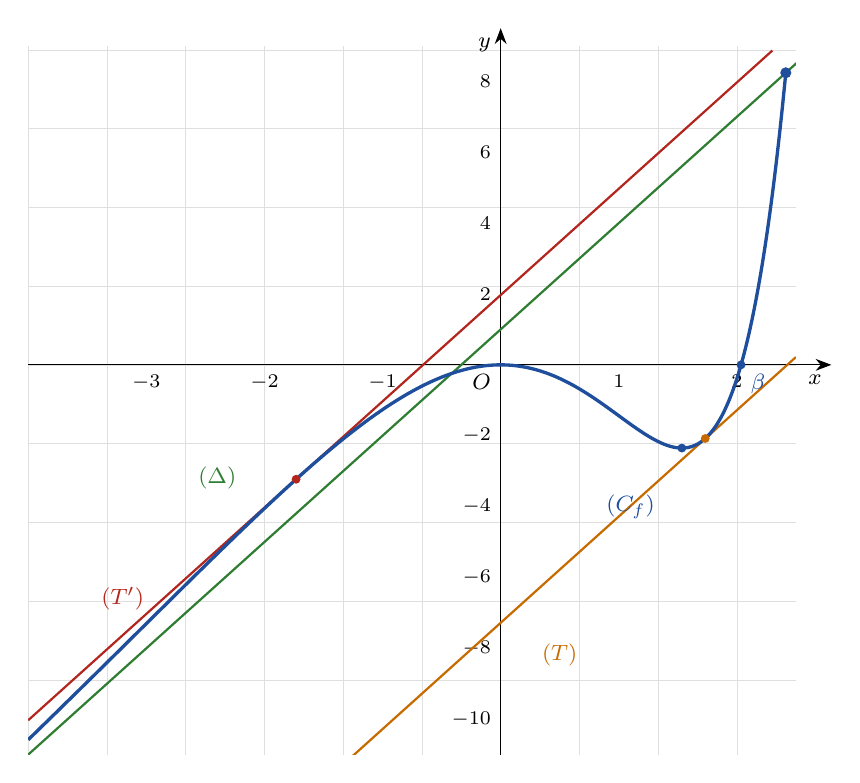
\begin{tikzpicture}[x=1.5cm,y=0.45cm,font=\footnotesize]
 \draw[gray!25,very thin] (-4,-11) grid (2.5,9);
 \draw[-{Stealth[length=2mm]}] (-4,0)--(2.8,0) node[below left]{$x$};
 \draw[-{Stealth[length=2mm]}] (0,-11)--(0,9.5) node[below left]{$y$};
 \node[below left] at (0,0){$O$};
 \foreach \t in {-3,-2,-1,1,2} \node[below,font=\scriptsize] at (\t,0){$\t$};
 \foreach \t in {-10,-8,-6,-4,-2,2,4,6,8} \node[left,font=\scriptsize] at (0,\t){$\t$};
 \begin{scope}\clip (-4,-11) rectangle (2.5,9);
 \draw[cRem,thick] (-4,-11)--(2.6,8.8);
 \draw[cEx,thick] (-1.4,-11.48)--(2.5,0.22);
 \draw[cThm,thick] (-4,-10.03)--(2.3,8.87);
 \draw[cDef,very thick,domain=-4:2.4142,samples=250,smooth] plot (\x,{3*\x+1+(\x*\x-2*\x-1)*exp(\x)});
 \fill[cDef] (2.4142,8.2426) circle (2pt);
 \fill[cDef] (1.5339,-2.349) circle (1.6pt);
 \fill[cDef] (2.0352,0) circle (1.6pt) node[below right]{$\beta$};
 \fill[cEx] (1.7321,-2.079) circle (1.6pt);
 \fill[cThm] (-1.7321,-3.229) circle (1.6pt);
 \end{scope}
 \node[cRem] at (-2.4,-3.2){$(\Delta)$};
 \node[cThm] at (-3.2,-6.6){$(T')$};
 \node[cEx] at (0.5,-8.2){$(T)$};
 \node[cDef] at (1.1,-4){$(C_f)$};
\end{tikzpicture}\end{LTR}\end{center}

\QQ{5}
\pa $\lim\limits_{x\to0^{+}}\ln x=-\infty$ و $\lim\limits_{X\to-\infty}f(X)=-\infty$، إذن \bx{\lim\limits_{x\to0^{+}}h(x)=-\infty}.
$\lim\limits_{x\to+\infty}\ln x=+\infty$ و $\lim\limits_{X\to+\infty}f(X)=+\infty$، إذن \bx{\lim\limits_{x\to+\infty}h(x)=+\infty}.

\pb $h$ قابلة للاشتقاق على $]0;+\infty[$ و $h'(x)=\dfrac1x\,f'(\ln x)=\dfrac{g(\ln x)}{x}$، وإشارتها إشارة $g(\ln x)$:
\begin{itemize}
\item $g(\ln x)>0\iff \ln x<0$ أو $\ln x>\alpha\iff 0<x<1$ أو $x>e^{\alpha}$.
\item $g(\ln x)<0\iff 0<\ln x<\alpha\iff 1<x<e^{\alpha}$.
\end{itemize}
$h$ متزايدة تماما على $]0;1]$ وعلى $\left[e^{\alpha};+\infty\right[$، ومتناقصة تماما على $\left[1;e^{\alpha}\right]$؛ و $h(1)=f(0)=0$، $h\left(e^{\alpha}\right)=f(\alpha)$ ($e^{\alpha}\approx4{,}64$).
\begin{TAB}
\tkzTabInit[lgt=2,espcl=2.8]{$x$/1,$h'(x)$/1,$h(x)$/2}{$0$,$1$,$e^{\alpha}$,$+\infty$}
\tkzTabLine{d,+,z,-,z,+,}
\tkzTabVar{D-/$-\infty$,+/$0$,-/$f(\alpha)$,+/$+\infty$}
\end{TAB}
\end{hal}


% ===================== بكالوريا 2020 -- الموضوع الثاني -- رياضيات =====================
\Needspace{16\baselineskip}
\begin{tamrin}{بكالوريا 2020 -- الموضوع الثاني -- رياضيات}
\textbf{I)} الدالتان $g$ و $h$ معرفتان على المجال $]{-}\infty;0]$ كما يلي: $g(x)=-2e^{x}$ و $h(x)=x\left(e^{x}+1\right)$.

حدد إشارة كل من $g(x)$ و $h(x)$ على المجال $]{-}\infty;0]$.

\textbf{II)} الدالة العددية $f$ معرفة على المجال $]{-}\infty;0]$ كما يلي: $f(x)=(x-3)e^{x}+\dfrac12x^2$، و $(C_f)$ تمثيلها البياني في المستوي المنسوب إلى المعلم المتعامد والمتجانس $(O;\vec i,\vec j)$.
\QQ{1}
\begin{sq}
\qa بين أنه من أجل كل عدد حقيقي $x$ من المجال $]{-}\infty;0]$: $f'(x)=h(x)+g(x)$.
\qb استنتج اتجاه تغير الدالة $f$ على المجال $]{-}\infty;0]$.
\end{sq}
\QQ{2} أحسب $f(0)$ و $\lim\limits_{x\to-\infty}f(x)$، ثم شكل جدول تغيرات الدالة $f$.
\QQ{3} بين أن المعادلة $f(x)=0$ تقبل حلا وحيدا $\alpha$ في المجال $]{-}\infty;0]$، ثم تحقق أن: $-1{,}5<\alpha<-1{,}4$.
\QQ{4} $(P)$ هو التمثيل البياني للدالة $x\mapsto\dfrac12x^2$ على المجال $]{-}\infty;0]$.
\begin{sq}
\qa أحسب $\lim\limits_{x\to-\infty}\left[f(x)-\dfrac12x^2\right]$، ثم فسر النتيجة بيانيا.
\qb أدرس الوضع النسبي للمنحنيين $(C_f)$ و $(P)$.
\qc أنشئ $(P)$ ثم المنحنى $(C_f)$ على المجال $]{-}\infty;0]$.
\end{sq}
\QQ{5} ليكن $m$ وسيطا حقيقيا. ناقش بيانيا وحسب قيم $m$ عدد حلول المعادلة $|f(x)|=e^{m}$ في المجال $]{-}\infty;0]$.
\end{tamrin}

\begin{hal}
\textbf{الجزء الأول:}
\begin{itemize}
\item $e^{x}>0$ إذن \bx{g(x)=-2e^{x}<0} على $]{-}\infty;0]$.
\item $e^{x}+1>0$، فإشارة $h(x)$ هي إشارة $x$: \bx{h(x)\le0} على $]{-}\infty;0]$، وتنعدم عند $0$ فقط.
\end{itemize}

\textbf{الجزء الثاني:}

\QQ{1}
\pa $f'(x)=e^{x}+(x-3)e^{x}+x=(x-2)e^{x}+x$.
و $h(x)+g(x)=xe^{x}+x-2e^{x}=(x-2)e^{x}+x$، إذن \bx{f'(x)=h(x)+g(x)}.

\pb على $]{-}\infty;0]$: $h(x)\le0$ و $g(x)<0$، إذن $f'(x)<0$: $f$ متناقصة تماما على $]{-}\infty;0]$.

\QQ{2} $f(0)=(0-3)\times1+0$ أي \bx{f(0)=-3}.
$(x-3)e^{x}=xe^{x}-3e^{x}$ يؤول إلى $0$ عند $-\infty$ (التزايد المقارن)، و $\lim\limits_{x\to-\infty}\dfrac12x^2=+\infty$، إذن \bx{\lim\limits_{x\to-\infty}f(x)=+\infty}.
\begin{TAB}
\tkzTabInit[lgt=2,espcl=5]{$x$/1,$f'(x)$/1,$f(x)$/2}{$-\infty$,$0$}
\tkzTabLine{,-,}
\tkzTabVar{+/$+\infty$,-/$-3$}
\end{TAB}

\QQ{3} $f$ مستمرة ومتناقصة تماما على $]{-}\infty;0]$، وتأخذ قيمها في $[-3;+\infty[$ الذي يحوي $0$، إذن المعادلة $f(x)=0$ تقبل حلا وحيدا $\alpha$ في $]{-}\infty;0]$.
$f(-1{,}5)\approx0{,}121>0$ و $f(-1{,}4)\approx-0{,}105<0$، إذن \bx{-1{,}5<\alpha<-1{,}4} ($\alpha\approx-1{,}447$).

\QQ{4}
\pa $f(x)-\dfrac12x^2=(x-3)e^{x}=xe^{x}-3e^{x}$، إذن \bx{\lim\limits_{x\to-\infty}\left[f(x)-\dfrac12x^2\right]=0}.

\textbf{التفسير:} المنحنيان $(C_f)$ و $(P)$ متقاربان بجوار $-\infty$ ($(P)$ منحنى مقارب لـ $(C_f)$ عند $-\infty$).

\pb على $]{-}\infty;0]$: $x-3<0$ و $e^{x}>0$، إذن $f(x)-\dfrac12x^2<0$:
\begin{TAB}
\tkzTabInit[lgt=3,espcl=5]{$x$/1,$f(x)-\frac12x^2$/1,\mbox{\ar{الوضع النسبي}}/1.2}{$-\infty$,$0$}
\tkzTabLine{,-,}
\tkzTabLine{,\mbox{\ar{$(C_f)$ تحت $(P)$}},}
\end{TAB}

\pc \textbf{الإنشاء:}
\begin{GR}{-3.6}{0.6}{-3.5}{6.5}{0.85}
 \Ticks{-3,-2,-1}{-3,-2,-1,1,2,3,4,5,6}
 \draw[cRem,thick,domain=-3.6:0,samples=100,smooth] plot (\x,{0.5*\x*\x});
 \draw[cDef,very thick,domain=-3.6:0,samples=200,smooth] plot (\x,{(\x-3)*exp(\x)+0.5*\x*\x});
 \fill[cDef] (0,-3) circle (1.8pt);
 \fill[cDef] (-1.4467,0) circle (1.6pt) node[above right]{$\alpha$};
 \draw[gray,dashed] (-3.6,3)--(0.6,3) node[pos=0.95,above]{$y=3$};
 \node[cRem] at (-2.6,4.6){$(P)$};
 \node[cDef] at (-1.2,-1.3){$(C_f)$};
\end{GR}

\QQ{5} $|f(x)|=e^{m}\iff f(x)=e^{m}$ أو $f(x)=-e^{m}$ (مع $e^{m}>0$). نستعمل تقاطع $(C_f)$ مع المستقيمين $y=e^{m}$ و $y=-e^{m}$:
\begin{itemize}
\item المعادلة $f(x)=e^{m}$: بما أن $e^{m}>0\ge-3$ فلها حل وحيد (في $]{-}\infty;\alpha[$).
\item المعادلة $f(x)=-e^{m}$: لها حل وحيد (في $]\alpha;0]$) إذا كان $-3\le-e^{m}<0$ أي $e^{m}\le3$ أي $m\le\ln3$، ولا حل لها إذا كان $m>\ln3$.
\end{itemize}
إذن:
\bxt{إذا كان $m\le\ln3$: حلان}\quad ؛ \quad \bxt{إذا كان $m>\ln3$: حل وحيد} ($\ln3\approx1{,}10$).
\end{hal}


% ===================== بكالوريا 2019 -- الموضوع الثاني -- رياضيات =====================
\Needspace{16\baselineskip}
\begin{tamrin}{بكالوريا 2019 -- الموضوع الثاني -- رياضيات}
\textbf{I)} $f_k$ الدالة العددية المعرفة على $\R$ كما يلي: $f_k(x)=(x+1)^2e^{-kx}$، و $k$ وسيط حقيقي. $(C_k)$ المنحنى الممثل للدالة $f_k$ في المستوي المنسوب إلى المعلم المتعامد والمتجانس $(O;\vec i,\vec j)$.
\QQ{1} بين أن كل المنحنيات $(C_k)$ تمر من نقطتين ثابتتين يطلب تعيينهما.
\QQ{2} أحسب نهايتي الدالة $f_k$ عند $-\infty$ وعند $+\infty$. (ناقش حسب قيم الوسيط الحقيقي $k$).
\QQ{3}
\begin{sq}
\qa أحسب $f_k'(x)$، ثم حدد حسب قيم الوسيط الحقيقي $k$ اتجاه تغير الدالة $f_k$.
\qb شكل جدول تغيرات الدالة $f_k$ من أجل $k$ عدد حقيقي موجب تماما.
\end{sq}
\QQ{4} ناقش حسب قيم الوسيط الحقيقي $k$ الأوضاع النسبية للمنحنيين $(C_k)$ و $(C_{k+1})$.

\textbf{II)} $f$ الدالة المعرفة على $\R$ بـ: $f(x)=(x+1)^2e^{-2x}$، و $(C_f)$ تمثيلها البياني في المستوي المنسوب إلى المعلم المتعامد والمتجانس $(O;\vec i,\vec j)$.
\QQ{1} شكل جدول تغيرات الدالة $f$، ثم أرسم المنحنى $(C_f)$ على المجال $\left[-\frac32;+\infty\right[$.
\QQ{2}
\begin{sq}
\qa بين أن المعادلة $f(x)=1$ تقبل في $\R$ حلين أحدهما $\alpha$ بحيث: $-1{,}28<\alpha<-1{,}27$.
\qb عين قيم العدد الحقيقي $m$ التي من أجلها تقبل المعادلة $\left|\dfrac{x+1}{e^{x}}\right|=\left|\dfrac{m+1}{e^{m}}\right|$ حلا وحيدا.
\end{sq}
\end{tamrin}

\begin{hal}
\textbf{الجزء الأول:}

\QQ{1} ليكن $a\neq b$ عددين حقيقيين. $f_a(x)=f_b(x)\iff(x+1)^2\left(e^{-ax}-e^{-bx}\right)=0\iff x=-1$ أو $e^{-ax}=e^{-bx}$.
و $e^{-ax}=e^{-bx}\iff(b-a)x=0\iff x=0$.
$f_k(-1)=0$ و $f_k(0)=1$ من أجل كل $k$، إذن كل المنحنيات $(C_k)$ تمر من النقطتين: \bx{A(-1;0)} و \bx{B(0;1)}.

\QQ{2} لدينا $\lim\limits_{x\to\pm\infty}(x+1)^2=+\infty$.
\begin{itemize}
\item \textbf{$k=0$:} $f_0(x)=(x+1)^2$، إذن $\lim\limits_{x\to-\infty}f_0(x)=\lim\limits_{x\to+\infty}f_0(x)=+\infty$.
\item \textbf{$k>0$:} عند $-\infty$: $-kx\to+\infty$ فـ $e^{-kx}\to+\infty$، إذن $\lim\limits_{x\to-\infty}f_k(x)=+\infty$.
عند $+\infty$: $f_k(x)=\left(\dfrac{x+1}{x}\right)^2\times\dfrac{1}{k^2}(kx)^2e^{-kx}$، وبوضع $t=kx\to+\infty$: $\lim\limits_{t\to+\infty}t^2e^{-t}=0$ (التزايد المقارن)، إذن $\lim\limits_{x\to+\infty}f_k(x)=0$.
\item \textbf{$k<0$:} عند $+\infty$: $-kx\to+\infty$، إذن $\lim\limits_{x\to+\infty}f_k(x)=+\infty$.
عند $-\infty$: بوضع $t=kx\to+\infty$ نفس الحساب يعطي $\lim\limits_{x\to-\infty}f_k(x)=0$.
\end{itemize}
\begin{center}\renewcommand{\arraystretch}{1.7}
\begin{tabular}{|c|c|c|c|}\hline
\rowcolor{cSec!12} $k$ & $k<0$ & $k=0$ & $k>0$\\\hline
$\lim\limits_{x\to-\infty}f_k(x)$ & $0$ & $+\infty$ & $+\infty$\\\hline
$\lim\limits_{x\to+\infty}f_k(x)$ & $+\infty$ & $+\infty$ & $0$\\\hline
\end{tabular}
\end{center}

\QQ{3}
\pa $f_k'(x)=2(x+1)e^{-kx}-k(x+1)^2e^{-kx}$، أي: \bx{f_k'(x)=(x+1)\left(2-k-kx\right)e^{-kx}}.
\begin{itemize}
\item \textbf{$k=0$:} $f_0'(x)=2(x+1)$: $f_0$ متناقصة تماما على $]{-}\infty;-1]$ ومتزايدة تماما على $[-1;+\infty[$.
\item \textbf{$k\neq0$:} $f_k'(x)$ تنعدم عند $-1$ وعند $x_k=\dfrac{2-k}{k}=\dfrac2k-1$، و $f_k'(x)=-k(x+1)(x-x_k)e^{-kx}$.
\begin{itemize}
\item $k>0$: $x_k>-1$، و $f_k'(x)>0$ بين الجذرين فقط: $f_k$ متناقصة تماما على $]{-}\infty;-1]$ وعلى $[x_k;+\infty[$، ومتزايدة تماما على $[-1;x_k]$.
\item $k<0$: $x_k<-1$، و $f_k'(x)<0$ بين الجذرين فقط: $f_k$ متزايدة تماما على $]{-}\infty;x_k]$ وعلى $[-1;+\infty[$، ومتناقصة تماما على $[x_k;-1]$.
\end{itemize}
\end{itemize}

\pb من أجل $k>0$: $f_k(-1)=0$ و $f_k\!\left(\dfrac2k-1\right)=\dfrac{4}{k^2}e^{-k\left(\frac2k-1\right)}=\dfrac{4e^{k-2}}{k^2}$.
\begin{TAB}
\tkzTabInit[lgt=2,espcl=2.8]{$x$/1,$f_k'(x)$/1,$f_k(x)$/2}{$-\infty$,$-1$,$\frac2k-1$,$+\infty$}
\tkzTabLine{,-,z,+,z,-,}
\tkzTabVar{+/$+\infty$,-/$0$,+/$\frac{4e^{k-2}}{k^2}$,-/$0$}
\end{TAB}

\QQ{4} $f_{k+1}(x)-f_k(x)=(x+1)^2e^{-kx}\left(e^{-x}-1\right)$. بما أن $(x+1)^2\ge0$ و $e^{-kx}>0$ فالإشارة هي إشارة $e^{-x}-1$، الموجبة لما $x<0$ والسالبة لما $x>0$ (مع الانعدام عند $-1$ و $0$):
\begin{TAB}
\tkzTabInit[lgt=3.4,espcl=3.2]{$x$/1,$f_{k+1}(x)-f_k(x)$/1,\mbox{\ar{الوضع النسبي}}/1.2}{$-\infty$,$-1$,$0$,$+\infty$}
\tkzTabLine{,+,z,+,z,-,}
\tkzTabLine{,\mbox{\ar{$(C_{k+1})$ فوق $(C_k)$}},t,\mbox{\ar{$(C_{k+1})$ فوق $(C_k)$}},t,\mbox{\ar{$(C_{k+1})$ تحت $(C_k)$}},}
\end{TAB}
النتيجة لا تتعلق بـ $k$: من أجل كل $k$، $(C_{k+1})$ فوق $(C_k)$ على $]{-}\infty;0[$ (ما عدا $A$)، وتحته على $]0;+\infty[$، ويتقاطعان في $A(-1;0)$ و $B(0;1)$.

\textbf{الجزء الثاني:} $f=f_2$، و $x_2=\frac22-1=0$، و $f(0)=\dfrac{4e^{0}}{4}=1$.

\QQ{1} حسب الجزء الأول ($k=2>0$):
\begin{TAB}
\tkzTabInit[lgt=2,espcl=2.8]{$x$/1,$f'(x)$/1,$f(x)$/2}{$-\infty$,$-1$,$0$,$+\infty$}
\tkzTabLine{,-,z,+,z,-,}
\tkzTabVar{+/$+\infty$,-/$0$,+/$1$,-/$0$}
\end{TAB}
المستقيم $y=0$ مقارب لـ $(C_f)$ عند $+\infty$؛ $f\left(-\frac32\right)=\frac14e^{3}\approx5{,}02$.
\begin{GR}{-1.5}{4.5}{-0.5}{5.2}{1.2}
 \Ticks{-1,1,2,3,4}{1,2,3,4,5}
 \draw[cDef,very thick,domain=-1.5:4.5,samples=250,smooth] plot (\x,{(\x+1)*(\x+1)*exp(-2*\x)});
 \fill[cDef] (-1,0) circle (1.6pt) node[below]{$A$};
 \fill[cDef] (0,1) circle (1.6pt) node[above right]{$B$};
 \draw[gray,dashed] (-1.5,1)--(4.5,1);
 \fill[cThm] (-1.2785,1) circle (1.6pt) node[above left]{$\alpha$};
 \node[cDef] at (-0.7,3.8){$(C_f)$};
\end{GR}

\QQ{2}
\pa \begin{itemize}
\item على $]{-}\infty;-1]$: $f$ مستمرة ومتناقصة تماما من $+\infty$ إلى $0$، إذن المعادلة $f(x)=1$ تقبل حلا وحيدا $\alpha$؛ و $f(-1{,}28)\approx1{,}014>1$، $f(-1{,}27)\approx0{,}924<1$، إذن \bx{-1{,}28<\alpha<-1{,}27}.
\item على $[-1;0]$: $f$ متزايدة تماما من $0$ إلى $1$، والحل الوحيد هو $x=0$.
\item على $]0;+\infty[$: $f(x)<f(0)=1$، لا حلول.
\end{itemize}
إذن المعادلة $f(x)=1$ تقبل حلين: $\alpha$ و $0$.

\pb الطرفان موجبان، إذن بالتربيع:
\[\left|\frac{x+1}{e^{x}}\right|=\left|\frac{m+1}{e^{m}}\right|\iff(x+1)^2e^{-2x}=(m+1)^2e^{-2m}\iff f(x)=f(m)\]
حلولها فواصل نقط تقاطع $(C_f)$ مع المستقيم الأفقي $y=f(m)$، و $x=m$ حل دائما:
\begin{itemize}
\item $f(m)=0$: حل وحيد $-1$. \quad $0<f(m)<1$: ثلاثة حلول. \quad $f(m)=1$: حلان.
\item $f(m)>1$: حل وحيد (في $]{-}\infty;\alpha[$)، و $f(m)>1\iff m<\alpha$.
\end{itemize}
إذن: \bx{m\in\left]{-}\infty;\alpha\right[\cup\{-1\}}.
\end{hal}


% ===================== بكالوريا 2018 -- الموضوع الثاني -- رياضيات =====================
\Needspace{16\baselineskip}
\begin{tamrin}{بكالوريا 2018 -- الموضوع الثاني -- رياضيات}
\textbf{I)} $g$ الدالة العددية المعرفة على المجال $]0;+\infty[$ كما يلي: $g(x)=\left(1+x+x^2\right)e^{-\frac1x}-1$.
\QQ{1} بين أنه من أجل كل $x$ من المجال $]0;+\infty[$: $g'(x)=\dfrac{(x+1)\left(2x^2+1\right)}{x^2}e^{-\frac1x}$، واستنتج اتجاه تغير الدالة $g$ على المجال $]0;+\infty[$.
\QQ{2} بين أن المعادلة $g(x)=0$ تقبل حلا وحيدا $\alpha$ حيث $0{,}9<\alpha<1$، واستنتج إشارة $g(x)$ على المجال $]0;+\infty[$.

\textbf{II)} $f$ الدالة العددية المعرفة على المجال $]0;+\infty[$ كما يلي: $f(x)=\dfrac1x+(1+x)e^{-\frac1x}$، و $(C_f)$ تمثيلها البياني في المستوي المنسوب إلى المعلم المتعامد والمتجانس $(O;\vec i,\vec j)$.
\QQ{1}
\begin{sq}
\qa أحسب $\lim\limits_{x\to0^{+}}f(x)$ و $\lim\limits_{x\to+\infty}f(x)$.
\qb بين أنه من أجل كل $x$ من المجال $]0;+\infty[$: $f'(x)=\dfrac{g(x)}{x^2}$، واستنتج اتجاه تغير الدالة $f$، ثم شكل جدول تغيراتها.
\end{sq}
\QQ{2} بين أن: $\lim\limits_{x\to+\infty}\left(xe^{-\frac1x}-x\right)=-1$ (يمكن وضع $t=-\frac1x$) ثم استنتج أن المستقيم $(\Delta)$ ذا المعادلة $y=x$ مقارب للمنحنى $(C_f)$ عند $+\infty$.
\QQ{3} $h$ الدالة العددية المعرفة على المجال $]0;+\infty[$ كما يلي: $h(x)=\dfrac1x-1+e^{-\frac1x}$.
\begin{sq}
\qa أحسب $\lim\limits_{x\to+\infty}h(x)$ وأدرس اتجاه تغير الدالة $h$ واستنتج إشارة $h(x)$ على المجال $]0;+\infty[$.
\qb تحقق أن: $f(x)-x=(1+x)h(x)$، ثم استنتج الوضعية النسبية لـ $(C_f)$ بالنسبة للمستقيم $(\Delta)$.
\end{sq}
\QQ{4} أرسم المستقيم $(\Delta)$ والمنحنى $(C_f)$. (نأخذ $f(\alpha)\approx1{,}73$).
\QQ{5} $(u_n)$ متتالية عددية معرفة على $\N^{*}$ بحدها العام $u_n$ حيث: $u_n=\dfrac{n}{n+1}f\!\left(\dfrac1n\right)-\dfrac{n^2}{n+1}$.
\begin{sq}
\qa أكتب $u_n$ بدلالة $n$ ثم بين أن المتتالية $(u_n)$ هندسية يطلب تعيين أساسها وحدها الأول $u_1$.
\qb أحسب بدلالة $n$ المجموع $S_n$ حيث:
\[S_n=\left(\frac12f(1)-\frac12\right)+\left(\frac23f\!\left(\frac12\right)-\frac13\right)+\left(\frac34f\!\left(\frac13\right)-\frac14\right)+\dots+\left(\frac{n}{n+1}f\!\left(\frac1n\right)-\frac1{n+1}\right)\]
\end{sq}
\end{tamrin}

\begin{hal}
\textbf{الجزء الأول:}

\QQ{1} $\left(e^{-\frac1x}\right)'=\dfrac1{x^2}e^{-\frac1x}$، إذن:
\begin{align*}
g'(x)&=(1+2x)e^{-\frac1x}+\left(1+x+x^2\right)\frac1{x^2}e^{-\frac1x}\\
&=\frac{2x^3+x^2+x^2+x+1}{x^2}e^{-\frac1x}=\frac{2x^3+2x^2+x+1}{x^2}e^{-\frac1x}
\end{align*}
و $(x+1)\left(2x^2+1\right)=2x^3+2x^2+x+1$، إذن \bx{g'(x)=\dfrac{(x+1)\left(2x^2+1\right)}{x^2}e^{-\frac1x}}.
على $]0;+\infty[$ كل العوامل موجبة تماما، إذن $g'(x)>0$: \bxt{$g$ متزايدة تماما على $]0;+\infty[$}.

\QQ{2} $g$ مستمرة ومتزايدة تماما على $[0{,}9;1]$، و $g(0{,}9)\approx-0{,}108<0$، $g(1)=3e^{-1}-1\approx0{,}104>0$، إذن حسب مبرهنة القيم المتوسطة (والرتابة التامة على $]0;+\infty[$) المعادلة $g(x)=0$ تقبل حلا وحيدا \bx{0{,}9<\alpha<1} ($\alpha\approx0{,}952$).
\begin{TAB}
\tkzTabInit[lgt=2,espcl=3.5]{$x$/1,$g(x)$/1}{$0$,$\alpha$,$+\infty$}
\tkzTabLine{d,-,z,+,}
\end{TAB}

\textbf{الجزء الثاني:}

\QQ{1}
\pa \textbf{عند $0^{+}$:} $\lim\limits_{x\to0^{+}}\left(-\frac1x\right)=-\infty$ فـ $\lim\limits_{x\to0^{+}}e^{-\frac1x}=0$، و $\lim\limits_{x\to0^{+}}\frac1x=+\infty$، إذن \bx{\lim\limits_{x\to0^{+}}f(x)=+\infty} (المستقيم $x=0$ مقارب عمودي).

\textbf{عند $+\infty$:} $\lim\limits_{x\to+\infty}e^{-\frac1x}=e^{0}=1$ و $\lim\limits_{x\to+\infty}(1+x)=+\infty$، إذن \bx{\lim\limits_{x\to+\infty}f(x)=+\infty}.

\pb
\[f'(x)=-\frac1{x^2}+e^{-\frac1x}+(1+x)\frac1{x^2}e^{-\frac1x}=\frac{-1+x^2e^{-\frac1x}+(1+x)e^{-\frac1x}}{x^2}=\frac{\left(1+x+x^2\right)e^{-\frac1x}-1}{x^2}\]
إذن \bx{f'(x)=\dfrac{g(x)}{x^2}}، وإشارتها إشارة $g(x)$: $f$ متناقصة تماما على $]0;\alpha]$ ومتزايدة تماما على $[\alpha;+\infty[$.
\begin{TAB}
\tkzTabInit[lgt=2,espcl=3.5]{$x$/1,$f'(x)$/1,$f(x)$/2}{$0$,$\alpha$,$+\infty$}
\tkzTabLine{d,-,z,+,}
\tkzTabVar{D+/$+\infty$,-/$f(\alpha)$,+/$+\infty$}
\end{TAB}

\QQ{2} نضع $t=-\frac1x$، أي $x=-\frac1t$؛ لما $x\to+\infty$ فإن $t\to0^{-}$:
\[xe^{-\frac1x}-x=-\frac1t\left(e^{t}-1\right)=-\frac{e^{t}-1}{t}\]
و $\lim\limits_{t\to0}\dfrac{e^{t}-1}{t}=1$ (العدد المشتق لـ $\exp$ عند $0$)، إذن \bx{\lim\limits_{x\to+\infty}\left(xe^{-\frac1x}-x\right)=-1}.

ومنه: $f(x)-x=\dfrac1x+e^{-\frac1x}+\left(xe^{-\frac1x}-x\right)$ يؤول إلى $0+1-1=0$، إذن $(\Delta):y=x$ مقارب مائل لـ $(C_f)$ عند $+\infty$.

\QQ{3}
\pa $\lim\limits_{x\to+\infty}h(x)=0-1+1$ أي \bx{\lim\limits_{x\to+\infty}h(x)=0}.
$h'(x)=-\dfrac1{x^2}+\dfrac1{x^2}e^{-\frac1x}=\dfrac{e^{-\frac1x}-1}{x^2}$، وبما أن $-\frac1x<0$ فإن $e^{-\frac1x}<1$، إذن $h'(x)<0$: $h$ متناقصة تماما على $]0;+\infty[$.
وبما أنها متناقصة تماما ونهايتها $0$ عند $+\infty$ فإن \bx{h(x)>0} من أجل كل $x>0$.

\pb $(1+x)h(x)=\dfrac1x-1+e^{-\frac1x}+1-x+xe^{-\frac1x}=\dfrac1x+(1+x)e^{-\frac1x}-x=f(x)-x$ \ok.
بما أن $1+x>0$ و $h(x)>0$ فإن $f(x)-x>0$:
\begin{TAB}
\tkzTabInit[lgt=3,espcl=5]{$x$/1,$f(x)-x$/1,\mbox{\ar{الوضع النسبي}}/1.2}{$0$,$+\infty$}
\tkzTabLine{d,+,}
\tkzTabLine{d,\mbox{\ar{$(C_f)$ فوق $(\Delta)$}},}
\end{TAB}

\QQ{4} \textbf{الرسم:} المقاربان $x=0$ و $y=x$، والذروة $(\alpha;f(\alpha))\approx(0{,}95;1{,}73)$.
\begin{GR}{-0.5}{4.5}{-0.5}{5.5}{1.1}
 \Ticks{1,2,3,4}{1,2,3,4,5}
 \draw[cRem,thick] (-0.5,-0.5)--(4.5,4.5);
 \draw[cDef,very thick,domain=0.18:4.5,samples=200,smooth] plot (\x,{1/\x+(1+\x)*exp(-1/\x)});
 \fill[cDef] (0.9521,1.7332) circle (1.6pt);
 \node[cRem] at (3.6,3.1){$(\Delta)$};
 \node[cDef] at (3,4.4){$(C_f)$};
\end{GR}

\Needspace{8\baselineskip}\QQ{5}
\pa $f\!\left(\frac1n\right)=n+\left(1+\frac1n\right)e^{-n}=n+\dfrac{n+1}{n}e^{-n}$، إذن:
\[u_n=\frac{n}{n+1}\left(n+\frac{n+1}{n}e^{-n}\right)-\frac{n^2}{n+1}=\frac{n^2}{n+1}+e^{-n}-\frac{n^2}{n+1}\]
أي \bx{u_n=e^{-n}}. و $\dfrac{u_{n+1}}{u_n}=\dfrac{e^{-n-1}}{e^{-n}}=e^{-1}$: $(u_n)$ هندسية أساسها \bx{q=e^{-1}} وحدها الأول \bx{u_1=e^{-1}}.

\pb الحد العام في $S_n$ هو: $\dfrac{p}{p+1}f\!\left(\frac1p\right)-\dfrac1{p+1}=u_p+\dfrac{p^2}{p+1}-\dfrac1{p+1}=u_p+\dfrac{(p-1)(p+1)}{p+1}=u_p+(p-1)$.
إذن:
\[S_n=\sum_{p=1}^{n}u_p+\sum_{p=1}^{n}(p-1)=e^{-1}\,\frac{1-e^{-n}}{1-e^{-1}}+\big(0+1+\dots+(n-1)\big)\]
\[\bx{S_n=\frac{1-e^{-n}}{e-1}+\frac{n(n-1)}{2}}\]
\end{hal}


% ===================== بكالوريا 2017 -- الموضوع الثاني -- رياضيات -- الدورة الاستثنائية =====================
\Needspace{16\baselineskip}
\begin{tamrin}{بكالوريا 2017 -- الموضوع الثاني -- رياضيات -- الدورة الاستثنائية}
المستوي منسوب إلى المعلم المتعامد والمتجانس $(O;\vec i,\vec j)$ حيث $\|\vec i\|=1cm$.

\textbf{I)} نعتبر الدالة العددية $f$ المعرفة على $\R$ كما يلي: $f(x)=(x+1)^2e^{-x}$، و $(C)$ تمثيلها البياني.
\QQ{1} أحسب $\lim\limits_{x\to-\infty}f(x)$ و $\lim\limits_{x\to+\infty}f(x)$.
\QQ{2} أدرس اتجاه تغير الدالة $f$ ثم شكل جدول تغيراتها.
\QQ{3} أثبت أن المنحنى $(C)$ يقبل نقطتي انعطاف يطلب تعيين إحداثييهما، أحسب $f(-2)$، ثم أرسم المنحنى $(C)$.

\textbf{II)} ليكن $m$ وسيطا حقيقيا، نعتبر الدالة $f_m$ المعرفة على $\R$ كما يلي: $f_m(x)=\left(x^2+mx+1\right)e^{-x}$، وليكن $(C_m)$ تمثيلها البياني في المعلم السابق.
\QQ{1} أثبت أن جميع المنحنيات $(C_m)$ تشمل نقطة ثابتة $\omega$ يطلب تعيين إحداثييها.
\QQ{2} أدرس اتجاه تغير الدالة $f_m$ واستنتج قيم $m$ التي من أجلها تقبل $f_m$ قيمتين حديتين يطلب تعيينهما.
\QQ{3} $M_m$ نقطة من $(C_m)$ فاصلتها $x_m$ حيث: $x_m=1-m$.
أثبت أنه عندما $m$ يمسح $\R$ فإن $M_m$ تنتمي إلى منحنى يطلب تعيين معادلة له.
\QQ{4} أدرس حسب قيم الوسيط $m$ حيث $m\neq2$ الوضعية النسبية للمنحنيين $(C)$ و $(C_m)$.
\end{tamrin}

\begin{hal}
\textbf{الجزء الأول:}

\QQ{1} \textbf{عند $-\infty$:} $\lim\limits_{x\to-\infty}(x+1)^2=+\infty$ و $\lim\limits_{x\to-\infty}e^{-x}=+\infty$، إذن \bx{\lim\limits_{x\to-\infty}f(x)=+\infty}.

\textbf{عند $+\infty$:} $f(x)=x^2e^{-x}+2xe^{-x}+e^{-x}$، وحسب التزايد المقارن $\lim\limits_{x\to+\infty}x^2e^{-x}=\lim\limits_{x\to+\infty}xe^{-x}=0$، إذن \bx{\lim\limits_{x\to+\infty}f(x)=0} (المستقيم $y=0$ مقارب أفقي عند $+\infty$).

\QQ{2} $f'(x)=2(x+1)e^{-x}-(x+1)^2e^{-x}=(x+1)(2-x-1)e^{-x}$، أي \bx{f'(x)=(x+1)(1-x)e^{-x}}.
$f$ متناقصة تماما على $]{-}\infty;-1]$ وعلى $[1;+\infty[$، ومتزايدة تماما على $[-1;1]$؛ $f(-1)=0$ و $f(1)=\dfrac4e\approx1{,}47$.
\begin{TAB}
\tkzTabInit[lgt=2,espcl=2.8]{$x$/1,$f'(x)$/1,$f(x)$/2}{$-\infty$,$-1$,$1$,$+\infty$}
\tkzTabLine{,-,z,+,z,-,}
\tkzTabVar{+/$+\infty$,-/$0$,+/$\frac4e$,-/$0$}
\end{TAB}

\QQ{3} $f'(x)=\left(1-x^2\right)e^{-x}$، إذن $f''(x)=-2xe^{-x}-\left(1-x^2\right)e^{-x}=\left(x^2-2x-1\right)e^{-x}$.
$f''(x)$ تنعدم مغيرة إشارتها عند $x=1-\sqrt2$ وعند $x=1+\sqrt2$:
\begin{TAB}
\tkzTabInit[lgt=2,espcl=2.8]{$x$/1,$f''(x)$/1}{$-\infty$,$1-\sqrt2$,$1+\sqrt2$,$+\infty$}
\tkzTabLine{,+,z,-,z,+,}
\end{TAB}
إذن $(C)$ يقبل نقطتي انعطاف:
\[\bx{I_1\left(1-\sqrt2;\left(6-4\sqrt2\right)e^{\sqrt2-1}\right)}\ ,\quad \bx{I_2\left(1+\sqrt2;\left(6+4\sqrt2\right)e^{-1-\sqrt2}\right)}\]
($I_1\approx(-0{,}41;0{,}52)$ و $I_2\approx(2{,}41;1{,}04)$). و $f(-2)=(-1)^2e^{2}$ أي \bx{f(-2)=e^2\approx7{,}39}.
\begin{GR}{-2.5}{7}{-0.5}{7.6}{1}
 \Ticks{-2,-1,1,2,3,4,5,6}{1,2,3,4,5,6,7}
 \draw[cDef,very thick,domain=-2.02:7,samples=250,smooth] plot (\x,{(\x+1)*(\x+1)*exp(-\x)});
 \fill[cDef] (-2,7.389) circle (1.6pt);
 \fill[cDef] (-1,0) circle (1.6pt);
 \fill[cDef] (1,1.4715) circle (1.6pt);
 \fill[cThm] (-0.4142,0.5192) circle (1.8pt) node[left]{$I_1$};
 \fill[cThm] (2.4142,1.0432) circle (1.8pt) node[above right]{$I_2$};
 \node[cDef] at (-0.9,4.5){$(C)$};
\end{GR}

\textbf{الجزء الثاني:}

\QQ{1} $f_m(x)=\left(x^2+1\right)e^{-x}+mxe^{-x}$. النقطة ثابتة إذا كان $f_m(x)$ لا يتعلق بـ $m$، أي $xe^{-x}=0$، أي $x=0$؛ و $f_m(0)=1$. إذن جميع المنحنيات $(C_m)$ تشمل النقطة \bx{\omega(0;1)}.

\QQ{2} $f_m'(x)=(2x+m)e^{-x}-\left(x^2+mx+1\right)e^{-x}=\left(-x^2+(2-m)x+m-1\right)e^{-x}$.
مميز $x^2-(2-m)x+1-m$ هو $(2-m)^2-4(1-m)=m^2$، وجذراه $1$ و $1-m$، إذن:
\[\bx{f_m'(x)=-(x-1)\big(x-(1-m)\big)e^{-x}}\]
\begin{itemize}
\item \textbf{$m=0$:} $f_0'(x)=-(x-1)^2e^{-x}\le0$: $f_0$ متناقصة تماما على $\R$ (لا تقبل قيما حدية).
\item \textbf{$m>0$} ($1-m<1$): $f_m$ متناقصة تماما على $]{-}\infty;1-m]$ وعلى $[1;+\infty[$، ومتزايدة تماما على $[1-m;1]$.
\item \textbf{$m<0$} ($1-m>1$): $f_m$ متناقصة تماما على $]{-}\infty;1]$ وعلى $[1-m;+\infty[$، ومتزايدة تماما على $[1;1-m]$.
\end{itemize}
(النهايات كما في الجزء الأول: $+\infty$ عند $-\infty$ و $0$ عند $+\infty$.)
\textbf{جدول التغيرات لما $m>0$:}
\begin{TAB}
\tkzTabInit[lgt=2,espcl=2.8]{$x$/1,$f_m'(x)$/1,$f_m(x)$/2}{$-\infty$,$1-m$,$1$,$+\infty$}
\tkzTabLine{,-,z,+,z,-,}
\tkzTabVar{+/$+\infty$,-/$(2-m)e^{m-1}$,+/$\frac{m+2}{e}$,-/$0$}
\end{TAB}
\Needspace{9\baselineskip}\textbf{جدول التغيرات لما $m<0$:}
\begin{TAB}
\tkzTabInit[lgt=2,espcl=2.8]{$x$/1,$f_m'(x)$/1,$f_m(x)$/2}{$-\infty$,$1$,$1-m$,$+\infty$}
\tkzTabLine{,-,z,+,z,-,}
\tkzTabVar{+/$+\infty$,-/$\frac{m+2}{e}$,+/$(2-m)e^{m-1}$,-/$0$}
\end{TAB}

إذن $f_m$ تقبل قيمتين حديتين \bxt{إذا وفقط إذا كان $m\neq0$}، وهما:
\[f_m(1)=\frac{m+2}{e}\qquad\text{;}\qquad f_m(1-m)=\big((1-m)^2+m(1-m)+1\big)e^{m-1}=(2-m)e^{m-1}\]

\QQ{3} $M_m\big(1-m;(2-m)e^{m-1}\big)$. نضع $X=1-m$ و $Y=(2-m)e^{m-1}$: $m=1-X$، ومنه $Y=(1+X)e^{-X}$.
عندما $m$ يمسح $\R$ فإن $X=1-m$ يمسح $\R$، إذن $M_m$ تنتمي إلى المنحنى ذي المعادلة: \bx{y=(x+1)e^{-x}}.

\QQ{4} $(C)=(C_2)$، و $f_m(x)-f(x)=(m-2)xe^{-x}$، إشارته إشارة $(m-2)x$:
\begin{TAB}
\tkzTabInit[lgt=4.2,espcl=3]{$x$/1,\mbox{\ar{$f_m(x)-f(x)$ لما $m>2$}}/1,\mbox{\ar{$f_m(x)-f(x)$ لما $m<2$}}/1}{$-\infty$,$0$,$+\infty$}
\tkzTabLine{,-,z,+,}
\tkzTabLine{,+,z,-,}
\end{TAB}
\begin{itemize}
\item $m>2$: $(C_m)$ تحت $(C)$ على $]{-}\infty;0[$ وفوقه على $]0;+\infty[$.
\item $m<2$: $(C_m)$ فوق $(C)$ على $]{-}\infty;0[$ وتحته على $]0;+\infty[$.
\item في الحالتين يتقاطعان في النقطة $\omega(0;1)$.
\end{itemize}
\end{hal}

% ===================== بكالوريا 2017 -- الموضوع الأول =====================
\begin{tamrin}{بكالوريا 2017 -- الموضوع الأول -- رياضيات}
نعتبر الدالة العددية $f$ المعرفة على $\R$ كما يلي: $f(x)=(-x^3+2x^2)e^{-x+1}$،
و $(C_f)$ تمثيلها البياني في المستوي المنسوب إلى المعلم المتعامد والمتجانس $(O;\vec i,\vec j)$.
\QQ{1}
\begin{sq}
\qa أحسب $\lim\limits_{x\to+\infty}f(x)$ و $\lim\limits_{x\to-\infty}f(x)$، ثم استنتج وجود مستقيم مقارب للمنحنى $(C_f)$ يطلب تعيين معادلة له.
\qb بيّن أنه من أجل كل عدد حقيقي $x$: $f'(x)=x(x^2-5x+4)e^{-x+1}$، ثم استنتج اتجاه تغيّر الدالة $f$ وشكّل جدول تغيّراتها.
\end{sq}
\QQ{2} أكتب معادلة المماس $(T)$ للمنحنى $(C_f)$ في النقطة ذات الفاصلة $2$.
\QQ{3} $h$ الدالة المعرفة على المجال $[0;+\infty[$ كما يلي: $h(x)=x^2e^{-x+2}-4$.
أدرس اتجاه تغيّر الدالة $h$ ثم استنتج إشارة $h(x)$، ثم حدّد عندئذ وضعية المنحنى $(C_f)$ بالنسبة إلى $(T)$ على المجال $[0;+\infty[$.
\QQ{4} أرسم المماس $(T)$ والمنحنى $(C_f)$ على المجال $[0;+\infty[$.
\QQ{5} نعتبر الوسيط الحقيقي $m$ والمعادلة ذات المجهول الحقيقي $x$ الموجب: \quad $f(x)=m(x-2)\ \ \ldots(E)$.
ناقش بيانيا وحسب قيم $m$ عدد حلول المعادلة $(E)$.
\QQ{6} $g$ الدالة العددية المعرفة على المجال $]0;+\infty[$ بـ: $g(x)=f\left(\dfrac1x\right)$.
اعتمادا على السؤال رقم (1)، شكّل جدول تغيّرات الدالة $g$.
\end{tamrin}

\begin{hal}
\QQ{1}
\pa \textbf{عند $+\infty$:} نكتب $f(x)=e\left(-x^3e^{-x}+2x^2e^{-x}\right)$.
حسب التزايد المقارن: $\lim\limits_{x\to+\infty}x^ne^{-x}=0$ من أجل كل عدد طبيعي $n$، إذن:
\[\bx{\lim_{x\to+\infty}f(x)=0}\]
\textbf{عند $-\infty$:} $-x^3+2x^2=-x^3\left(1-\dfrac2x\right)$ و $\lim\limits_{x\to-\infty}\left(-x^3\right)=+\infty$، إذن $\lim\limits_{x\to-\infty}(-x^3+2x^2)=+\infty$،
و $\lim\limits_{x\to-\infty}(-x+1)=+\infty$ إذن $\lim\limits_{x\to-\infty}e^{-x+1}=+\infty$، ومنه بالجداء:
\[\bx{\lim_{x\to-\infty}f(x)=+\infty}\]
\textbf{الاستنتاج:} بما أن $\lim\limits_{x\to+\infty}f(x)=0$ فإن المستقيم ذا المعادلة \bx{y=0} (محور الفواصل) مقارب أفقي للمنحنى $(C_f)$ عند $+\infty$.

\pb الدالة $f$ قابلة للاشتقاق على $\R$ (جداء دالة كثير حدود والدالة $x\mapsto e^{-x+1}$)، ومن أجل كل $x\in\R$:
\begin{align*}
f'(x)&=(-3x^2+4x)e^{-x+1}+(-x^3+2x^2)\times(-1)e^{-x+1}\\
&=\left(x^3-2x^2-3x^2+4x\right)e^{-x+1}=\left(x^3-5x^2+4x\right)e^{-x+1}
\end{align*}
إذن: \bx{f'(x)=x(x^2-5x+4)e^{-x+1}}.

\textbf{اتجاه التغيّر:} $e^{-x+1}>0$، إذن إشارة $f'(x)$ هي إشارة $x(x^2-5x+4)$.
للثلاثي $x^2-5x+4$ جذران: $1$ و $4$ (لأن $1-5+4=0$ وجداء الجذرين $4$)، أي $x^2-5x+4=(x-1)(x-4)$.
\begin{TAB}
\tkzTabInit[lgt=2.6,espcl=2.4]{$x$/1,$x$/1,$(x-1)(x-4)$/1,$f'(x)$/1}{$-\infty$,$0$,$1$,$4$,$+\infty$}
\tkzTabLine{,-,z,+,t,+,t,+,}
\tkzTabLine{,+,t,+,z,-,z,+,}
\tkzTabLine{,-,z,+,z,-,z,+,}
\end{TAB}
إذن: $f$ متناقصة تماما على كل من $]{-}\infty;0]$ و $[1;4]$، ومتزايدة تماما على كل من $[0;1]$ و $[4;+\infty[$.

$f(0)=0$ \ ،\ $f(1)=(-1+2)e^{0}=1$ \ ،\ $f(4)=(-64+32)e^{-3}=-32e^{-3}\approx-1{,}59$.
\begin{TAB}
\tkzTabInit[lgt=2,espcl=2.4]{$x$/1,$f'(x)$/1,$f(x)$/2.2}{$-\infty$,$0$,$1$,$4$,$+\infty$}
\tkzTabLine{,-,z,+,z,-,z,+,}
\tkzTabVar{+/$+\infty$,-/$0$,+/$1$,-/$-32e^{-3}$,+/$0$}
\end{TAB}

\QQ{2} معادلة المماس عند النقطة ذات الفاصلة $2$: $y=f'(2)(x-2)+f(2)$، حيث:
\[f(2)=(-8+8)e^{-1}=0\qquad;\qquad f'(2)=2\times(4-10+4)e^{-1}=-4e^{-1}=-\frac4e\]
إذن: \bx{(T):\ y=-\dfrac4e\,x+\dfrac8e}\ \ أي $y=-\dfrac4e(x-2)$.

\QQ{3} \textbf{اتجاه تغيّر $h$:} $h$ قابلة للاشتقاق على $[0;+\infty[$، و:
\[h'(x)=2xe^{-x+2}-x^2e^{-x+2}=x(2-x)e^{-x+2}\]
على $[0;+\infty[$: $x\geqslant0$ و $e^{-x+2}>0$، إذن إشارة $h'(x)$ هي إشارة $(2-x)$.
$h(0)=-4$ \ ،\ $h(2)=4e^{0}-4=0$ \ ،\ $\lim\limits_{x\to+\infty}h(x)=e^2\lim\limits_{x\to+\infty}x^2e^{-x}-4=-4$ (تزايد مقارن).
\begin{TAB}
\tkzTabInit[lgt=2,espcl=3.5]{$x$/1,$h'(x)$/1,$h(x)$/2}{$0$,$2$,$+\infty$}
\tkzTabLine{z,+,z,-,}
\tkzTabVar{-/$-4$,+/$0$,-/$-4$}
\end{TAB}
\textbf{إشارة $h(x)$:} القيمة العظمى للدالة $h$ على $[0;+\infty[$ هي $h(2)=0$، إذن:\par
\bxt{$h(x)<0$ من أجل كل $x\in[0;2[\cup]2;+\infty[$، و $h(2)=0$}.

\textbf{وضعية $(C_f)$ بالنسبة إلى $(T)$:} لدينا $f(x)=-x^2(x-2)e^{-x+1}$، ومنه:
\begin{align*}
f(x)-\left(-\frac4e(x-2)\right)&=(x-2)\left[-x^2e^{-x+1}+4e^{-1}\right]=(x-2)e^{-1}\left[-x^2e^{-x+2}+4\right]\\
&=-e^{-1}(x-2)\,h(x)
\end{align*}
بما أن $-e^{-1}h(x)\geqslant0$، فإن إشارة الفرق هي إشارة $(x-2)$:
\begin{TAB}
\tkzTabInit[lgt=3.4,espcl=3.5]{$x$/1,$x-2$/1,$-e^{-1}h(x)$/1,$f(x)-y_{(T)}$/1}{$0$,$2$,$+\infty$}
\tkzTabLine{,-,z,+,}
\tkzTabLine{,+,z,+,}
\tkzTabLine{,-,z,+,}
\end{TAB}
\begin{itemize}
\item على $[0;2[$: $(C_f)$ \textbf{تحت} المماس $(T)$.
\item على $]2;+\infty[$: $(C_f)$ \textbf{فوق} المماس $(T)$.
\item $(C_f)$ يقطع $(T)$ في النقطة $A(2;0)$؛ المماس يخترق المنحنى عندها فهي \textbf{نقطة انعطاف}.
\end{itemize}

\QQ{4} \textbf{الرسم:} المقارب $y=0$ عند $+\infty$، الذروتان $(1;1)$ و $(4;-32e^{-3})$، $O$ نقطة من $(C_f)$ بمماس أفقي، و $(T)$ يمر بـ $A(2;0)$ و $\left(0;\frac8e\right)\approx(0;2{,}94)$.
\begin{GR}{-0.5}{9.5}{-2.2}{3.2}{1.25}
 \Ticks{1,2,3,4,5,6,7,8,9}{-2,-1,1,2,3}
 \draw[cThm,thick,domain=-0.5:4] plot(\x,{-4/exp(1)*(\x-2)}); \node[cThm] at (0.75,2.4){$(T)$};
 \draw[cDef,very thick,domain=0:9.5,samples=160] plot(\x,{(-\x*\x*\x+2*\x*\x)*exp(-\x+1)});
 \draw[dashed,gray] (1,0)--(1,1)--(0,1);
 \draw[dashed,gray] (4,0)--(4,-1.593);
 \fill (1,1) circle (1.6pt) (4,-1.593) circle (1.6pt) (2,0) circle (1.6pt) node[above right]{$A$};
 \node[cDef] at (6.5,-1.45){$(C_f)$};
\end{GR}

\QQ{5} \textbf{المناقشة البيانية} ($x\in[0;+\infty[$): حلول $(E)$ هي فواصل نقط تقاطع $(C_f)$ مع المستقيم $(D_m):\ y=m(x-2)$ الذي يدور حول النقطة الثابتة $A(2;0)$ ومعامل توجيهه $m$.
\begin{itemize}
\item $x=2$ حل للمعادلة $(E)$ مهما كان $m$ (لأن $f(2)=0$).
\item من أجل $x\neq2$: $(E)\iff \dfrac{f(x)}{x-2}=m\iff -x^2e^{-x+1}=m$. نضع $k(x)=-x^2e^{-x+1}$:\ \ $k'(x)=x(x-2)e^{-x+1}$،
فـ $k$ متناقصة تماما على $[0;2]$ من $k(0)=0$ إلى $k(2)=-\dfrac4e$، ومتزايدة تماما على $[2;+\infty[$ من $-\dfrac4e$ نحو $0$ (دون بلوغه).
\end{itemize}
بيانيا: $(D_0)$ هو محور الفواصل، و $(D_{-4/e})$ هو المماس $(T)$. ومنه:
\begin{itemize}
\item $m>0$: $(D_m)$ يقطع $(C_f)$ في $A$ فقط: \bxt{حل وحيد $x=2$}.
\item $m=0$: \bxt{حلان: $x=0$ و $x=2$}.
\item $-\dfrac4e<m<0$: \bxt{ثلاثة حلول} (أحدها $2$، وحل في $]0;2[$ وحل في $]2;+\infty[$).
\item $m=-\dfrac4e$: $(D_m)=(T)$: \bxt{حل وحيد (مضاعف) $x=2$}.
\item $m<-\dfrac4e$: \bxt{حل وحيد $x=2$}.
\end{itemize}

\QQ{6} $g=f\circ u$ حيث $u(x)=\dfrac1x$، والدالة $u$ متناقصة تماما على $]0;+\infty[$ وتأخذ قيمها في $]0;+\infty[$، و $g'(x)=-\dfrac1{x^2}f'\left(\dfrac1x\right)$:
\begin{itemize}
\item $x\in]0;\tfrac14]\iff \tfrac1x\in[4;+\infty[$ حيث $f$ متزايدة: إذن $g$ \textbf{متناقصة} تماما على $]0;\tfrac14]$.
\item $x\in[\tfrac14;1]\iff \tfrac1x\in[1;4]$ حيث $f$ متناقصة: إذن $g$ \textbf{متزايدة} تماما على $[\tfrac14;1]$.
\item $x\in[1;+\infty[\iff \tfrac1x\in]0;1]$ حيث $f$ متزايدة: إذن $g$ \textbf{متناقصة} تماما على $[1;+\infty[$.
\end{itemize}
\textbf{النهايات:} $\lim\limits_{x\to0^+}\dfrac1x=+\infty$ إذن $\lim\limits_{x\to0^+}g(x)=\lim\limits_{t\to+\infty}f(t)=0$، و $\lim\limits_{x\to+\infty}\dfrac1x=0$ إذن $\lim\limits_{x\to+\infty}g(x)=f(0)=0$.
$g\left(\tfrac14\right)=f(4)=-32e^{-3}$ \ ،\ $g(1)=f(1)=1$.
\begin{TAB}
\tkzTabInit[lgt=2,espcl=2.8]{$x$/1,$g'(x)$/1,$g(x)$/2.2}{$0$,$\frac14$,$1$,$+\infty$}
\tkzTabLine{d,-,z,+,z,-,}
\tkzTabVar{D+/$0$,-/$-32e^{-3}$,+/$1$,-/$0$}
\end{TAB}
\end{hal}

% ===================== بكالوريا 2016 -- الموضوع الثاني =====================
\begin{tamrin}{بكالوريا 2016 -- الموضوع الثاني -- رياضيات}
\textbf{I)} $\varphi$ الدالة العددية المعرفة على $\R$ كما يلي: $\varphi(x)=(x^2-x+1)e^{-x+1}-1$.
\QQ{1}
\begin{sq}
\qa أحسب $\lim\limits_{x\to-\infty}\varphi(x)$ و $\lim\limits_{x\to+\infty}\varphi(x)$.
\qb أدرس اتجاه تغيّر الدالة $\varphi$ ثم شكّل جدول تغيّراتها.
\end{sq}
\QQ{2} بيّن أن المعادلة $\varphi(x)=0$ تقبل في $\R$ حلا $\alpha$ يختلف عن $1$، ثم تحقق أن: $2{,}79<\alpha<2{,}80$.
\QQ{3} استنتج إشارة $\varphi(x)$ على $\R$.

\textbf{II)} $f$ و $g$ الدالتان المعرفتان على $\R$ كما يلي: $f(x)=(2x-1)e^{-x+1}$ و $g(x)=\dfrac{2x-1}{x^2-x+1}$،
و $(C_f)$ و $(C_g)$ تمثيلاهما البيانيان في المستوي المنسوب إلى المعلم المتعامد والمتجانس $(O;\vec i,\vec j)$.
\QQ{1}
\begin{sq}
\qa أحسب $\lim\limits_{x\to-\infty}f(x)$ و $\lim\limits_{x\to+\infty}f(x)$.
\qb أدرس اتجاه تغيّر الدالة $f$ ثم شكّل جدول تغيّراتها.
\end{sq}
\QQ{2} بيّن أن للمنحنيين $(C_f)$ و $(C_g)$ مماسا مشتركا $(T)$ في النقطة ذات الفاصلة $1$، ثم جد معادلة له.
\QQ{3} أرسم المماس $(T)$ والمنحنى $(C_f)$.
\QQ{4}
\begin{sq}
\qa بيّن أنه من أجل كل عدد حقيقي $x$: $f(x)-g(x)=\dfrac{(2x-1)\varphi(x)}{x^2-x+1}$.
\qb أدرس إشارة الفرق $f(x)-g(x)$، ثم استنتج الوضع النسبي لـ $(C_f)$ و $(C_g)$.
\end{sq}
\end{tamrin}

\begin{hal}
\textbf{الجزء الأول:}

\QQ{1}
\pa \textbf{عند $-\infty$:} $\lim\limits_{x\to-\infty}(x^2-x+1)=+\infty$ و $\lim\limits_{x\to-\infty}e^{-x+1}=+\infty$، إذن:
\[\bx{\lim_{x\to-\infty}\varphi(x)=+\infty}\]
\textbf{عند $+\infty$:} $(x^2-x+1)e^{-x+1}=e\left(x^2e^{-x}-xe^{-x}+e^{-x}\right)$ و $\lim\limits_{x\to+\infty}x^ne^{-x}=0$ (تزايد مقارن)، إذن:
\[\bx{\lim_{x\to+\infty}\varphi(x)=-1}\]
(المستقيم $y=-1$ مقارب أفقي لمنحنى $\varphi$ عند $+\infty$.)

\pb $\varphi$ قابلة للاشتقاق على $\R$، و:
\[\varphi'(x)=(2x-1)e^{-x+1}-(x^2-x+1)e^{-x+1}=(-x^2+3x-2)e^{-x+1}=-(x-1)(x-2)e^{-x+1}\]
$e^{-x+1}>0$، إذن إشارة $\varphi'(x)$ هي إشارة $-(x-1)(x-2)$: موجبة بين الجذرين $1$ و $2$، وسالبة خارجهما.
$\varphi(1)=(1-1+1)e^{0}-1=0$ \ ،\ $\varphi(2)=3e^{-1}-1\approx0{,}10$.
\begin{TAB}
\tkzTabInit[lgt=2,espcl=3]{$x$/1,$\varphi'(x)$/1,$\varphi(x)$/2.2}{$-\infty$,$1$,$2$,$+\infty$}
\tkzTabLine{,-,z,+,z,-,}
\tkzTabVar{+/$+\infty$,-/$0$,+/$3e^{-1}-1$,-/$-1$}
\end{TAB}

\QQ{2} \begin{itemize}
\item على $]{-}\infty;2]$: القيمة الصغرى لـ $\varphi$ هي $\varphi(1)=0$، إذن $\varphi(x)>0$ من أجل $x\neq1$؛ فالحل الوحيد في هذا المجال هو $1$.
\item على $[2;+\infty[$: $\varphi$ مستمرة ومتناقصة تماما، و $\varphi(2)=3e^{-1}-1>0$ و $\lim\limits_{x\to+\infty}\varphi(x)=-1<0$، إذن حسب مبرهنة القيم المتوسطة تقبل المعادلة $\varphi(x)=0$ حلا وحيدا $\alpha$ في $]2;+\infty[$، و $\alpha\neq1$.
\end{itemize}
\textbf{التحقق:} $\varphi(2{,}79)\approx 0{,}0008>0$ و $\varphi(2{,}80)\approx-0{,}0016<0$، إذن \bx{2{,}79<\alpha<2{,}80} ($\alpha\approx2{,}793$).

\QQ{3} من جدول التغيّرات:
\begin{TAB}
\tkzTabInit[lgt=2,espcl=2.8]{$x$/1,$\varphi(x)$/1}{$-\infty$,$1$,$\alpha$,$+\infty$}
\tkzTabLine{,+,z,+,z,-,}
\end{TAB}
\par\bxt{$\varphi(x)\geqslant0$ على $]{-}\infty;\alpha]$ (تنعدم عند $1$ و $\alpha$)، و $\varphi(x)<0$ على $]\alpha;+\infty[$}.

\textbf{الجزء الثاني:}

\QQ{1}
\pa \textbf{عند $-\infty$:} $\lim\limits_{x\to-\infty}(2x-1)=-\infty$ و $\lim\limits_{x\to-\infty}e^{-x+1}=+\infty$، إذن \bx{\lim\limits_{x\to-\infty}f(x)=-\infty}.

\textbf{عند $+\infty$:} $f(x)=e\left(2xe^{-x}-e^{-x}\right)$ و $\lim\limits_{x\to+\infty}xe^{-x}=0$، إذن \bx{\lim\limits_{x\to+\infty}f(x)=0}: المستقيم $y=0$ مقارب أفقي لـ $(C_f)$ عند $+\infty$.

\pb $f'(x)=2e^{-x+1}-(2x-1)e^{-x+1}=(3-2x)e^{-x+1}$، وإشارتها إشارة $(3-2x)$:
$f$ متزايدة تماما على $\left]{-}\infty;\tfrac32\right]$ ومتناقصة تماما على $\left[\tfrac32;+\infty\right[$، و $f\left(\tfrac32\right)=2e^{-\frac12}\approx1{,}21$.
\begin{TAB}
\tkzTabInit[lgt=2,espcl=3.5]{$x$/1,$f'(x)$/1,$f(x)$/2}{$-\infty$,$\frac32$,$+\infty$}
\tkzTabLine{,+,z,-,}
\tkzTabVar{-/$-\infty$,+/$2e^{-\frac12}$,-/$0$}
\end{TAB}

\QQ{2} $f(1)=(2-1)e^{0}=1$ و $g(1)=\dfrac{1}{1-1+1}=1$: النقطة $(1;1)$ مشتركة بين $(C_f)$ و $(C_g)$.
\[f'(1)=(3-2)e^{0}=1\]
\[g'(x)=\frac{2(x^2-x+1)-(2x-1)^2}{(x^2-x+1)^2}=\frac{-2x^2+2x+1}{(x^2-x+1)^2}\ \Rightarrow\ g'(1)=\frac{1}{1}=1\]
بما أن $f(1)=g(1)$ و $f'(1)=g'(1)$ فللمنحنيين مماس مشترك $(T)$ في النقطة $(1;1)$، معادلته $y=1\times(x-1)+1$ أي: \bx{(T):\ y=x}.

\QQ{3} \textbf{الرسم} (رسمنا $(C_g)$ أيضا بخط متقطع للتوضيح):
\begin{GR}{-1}{7}{-3}{2.5}{1.4}
 \Ticks{1,2,3,4,5,6}{-2,-1,1,2}
 \draw[cThm,thick,domain=-1:2.5] plot(\x,{\x}); \node[cThm,left] at (2.2,2.2){$(T)$};
 \draw[cRem,thick,dashed,domain=-1:7,samples=120] plot(\x,{(2*\x-1)/(\x*\x-\x+1)});
 \draw[cDef,very thick,domain=-0.2:7,samples=150] plot(\x,{(2*\x-1)*exp(-\x+1)});
 \fill (1,1) circle (1.6pt) (1.5,1.213) circle (1.6pt) (0.5,0) circle (1.6pt);
 \draw[dashed,gray] (1.5,0)--(1.5,1.213);
 \node[cDef] at (5.3,0.55){$(C_f)$};
 \node[cRem] at (5.3,-0.35){$(C_g)$};
\end{GR}

\QQ{4}
\pa من أجل كل $x\in\R$ ($x^2-x+1>0$ لأن مميزه $-3<0$):
\[f(x)-g(x)=(2x-1)\left[e^{-x+1}-\frac{1}{x^2-x+1}\right]=(2x-1)\cdot\frac{(x^2-x+1)e^{-x+1}-1}{x^2-x+1}=\bx{\frac{(2x-1)\varphi(x)}{x^2-x+1}}\]
\pb $x^2-x+1>0$، إذن إشارة الفرق هي إشارة الجداء $(2x-1)\varphi(x)$:
\begin{TAB}
\tkzTabInit[lgt=2.6,espcl=2.4]{$x$/1,$2x-1$/1,$\varphi(x)$/1,$f(x)-g(x)$/1}{$-\infty$,$\frac12$,$1$,$\alpha$,$+\infty$}
\tkzTabLine{,-,z,+,t,+,t,+,}
\tkzTabLine{,+,t,+,z,+,z,-,}
\tkzTabLine{,-,z,+,z,+,z,-,}
\end{TAB}
\begin{itemize}
\item على $\left]{-}\infty;\tfrac12\right[$ و $]\alpha;+\infty[$: $(C_f)$ \textbf{تحت} $(C_g)$.
\item على $\left]\tfrac12;1\right[$ و $]1;\alpha[$: $(C_f)$ \textbf{فوق} $(C_g)$.
\item يتقاطعان في النقط ذات الفواصل $\tfrac12$ و $1$ (تماس) و $\alpha$.
\end{itemize}
\end{hal}

% ===================== بكالوريا 2015 -- الموضوع الثاني =====================
\begin{tamrin}{بكالوريا 2015 -- الموضوع الثاني -- رياضيات}
$f$ الدالة المعرفة بـ: $f(0)=0$، ومن أجل كل عدد حقيقي $x$ من المجال $]{-}\infty;0[$: $f(x)=(x-1)e^{\frac1x}$،
و $(C_f)$ تمثيلها البياني في المستوي المنسوب إلى المعلم المتعامد والمتجانس $(O;\vec i,\vec j)$.
\QQ{1} أدرس استمرارية الدالة $f$ عند $0$ من اليسار.
\QQ{2} أحسب $\lim\limits_{x\to0^-}\dfrac{f(x)}{x}$، ثم فسّر النتيجة هندسيا.
\QQ{3}
\begin{sq}
\qa أحسب $\lim\limits_{x\to-\infty}f(x)$.
\qb أدرس اتجاه تغيّر الدالة $f$، ثم شكّل جدول تغيّراتها.
\end{sq}
\QQ{4}
\begin{sq}
\qa بيّن أن: $\lim\limits_{x\to-\infty}\left[f(x)-x\right]=0$.
\qb استنتج أن المنحنى $(C_f)$ يقبل مستقيما مقاربا مائلا $(\Delta)$ عند $-\infty$، يطلب تعيين معادلة له.
\end{sq}
\QQ{5} $g$ الدالة المعرفة على $]{-}\infty;0[$ بـ: $g(x)=\dfrac{f(x)}{x}$.
\begin{sq}
\qa أحسب $\lim\limits_{x\to-\infty}g(x)$.
\qb أدرس اتجاه تغيّر الدالة $g$، ثم شكّل جدول تغيّراتها.
\end{sq}
\QQ{6}
\begin{sq}
\qa بيّن أنه من أجل كل عدد حقيقي $x$ من المجال $]{-}\infty;0[$: $f(x)>x$.
\qb استنتج وضعية المنحنى $(C_f)$ بالنسبة إلى المستقيم $(\Delta)$.
\qc أنشئ المنحنى $(C_f)$.
\end{sq}
\QQ{7} $m$ عدد حقيقي، و $h_m$ الدالة ذات المتغير الحقيقي $x$ المعرفة على المجال $]{-}\infty;0[$ بـ: $h_m(x)=xe^{\frac1x}-mx$.
\begin{sq}
\qa أحسب $h'_m(x)$ حيث $h'_m$ هي الدالة المشتقة للدالة $h_m$.
\qb باستعمال $(C_f)$، ناقش بيانيا وحسب قيم الوسيط الحقيقي $m$، عدد حلول المعادلة: $h'_m(x)=0$.
\end{sq}
\end{tamrin}

\begin{hal}
\QQ{1} عندما $x\to0^-$: $\dfrac1x\to-\infty$، إذن $\lim\limits_{x\to0^-}e^{\frac1x}=\lim\limits_{t\to-\infty}e^{t}=0$، و $\lim\limits_{x\to0^-}(x-1)=-1$، ومنه:
\[\lim_{x\to0^-}f(x)=-1\times0=0=f(0)\]
إذن: \bxt{الدالة $f$ مستمرة عند $0$ من اليسار}.

\QQ{2} $\dfrac{f(x)}{x}=\dfrac{x-1}{x}\,e^{\frac1x}=\left(1-\dfrac1x\right)e^{\frac1x}$. نضع $t=\dfrac1x$؛ عندما $x\to0^-$ فإن $t\to-\infty$:
\[\lim_{x\to0^-}\frac{f(x)}{x}=\lim_{t\to-\infty}(1-t)e^{t}=\lim_{t\to-\infty}\left(e^{t}-te^{t}\right)=0-0=0\]
(لأن $\lim\limits_{t\to-\infty}te^{t}=0$). إذن \bx{\lim_{x\to0^-}\dfrac{f(x)-f(0)}{x-0}=0}.

\textbf{التفسير الهندسي:} $f$ قابلة للاشتقاق عند $0$ من اليسار و $f'_g(0)=0$، فالمنحنى $(C_f)$ يقبل عند المبدأ $O$ \textbf{نصف مماس أفقي} (على يسار $O$).

\QQ{3}
\pa $\lim\limits_{x\to-\infty}\dfrac1x=0$ إذن $\lim\limits_{x\to-\infty}e^{\frac1x}=e^{0}=1$، و $\lim\limits_{x\to-\infty}(x-1)=-\infty$، ومنه \bx{\lim\limits_{x\to-\infty}f(x)=-\infty}.

\pb $f$ قابلة للاشتقاق على $]{-}\infty;0[$، ومن أجل كل $x<0$: $\left(e^{\frac1x}\right)'=-\dfrac1{x^2}e^{\frac1x}$، ومنه:
\[f'(x)=e^{\frac1x}+(x-1)\left(-\frac1{x^2}\right)e^{\frac1x}=\frac{x^2-x+1}{x^2}\,e^{\frac1x}\]
مميز $x^2-x+1$ هو $-3<0$ إذن $x^2-x+1>0$، و $x^2>0$ و $e^{\frac1x}>0$: إذن $f'(x)>0$ و \bxt{$f$ متزايدة تماما على $]{-}\infty;0]$}.
\begin{TAB}
\tkzTabInit[lgt=2,espcl=4]{$x$/1,$f'(x)$/1,$f(x)$/2}{$-\infty$,$0$}
\tkzTabLine{,+,z}
\tkzTabVar{-/$-\infty$,+/$0$}
\end{TAB}
(العدد المشتق من اليسار عند $0$ معدوم حسب السؤال 2.)

\QQ{4}
\pa $f(x)-x=xe^{\frac1x}-e^{\frac1x}-x=x\left(e^{\frac1x}-1\right)-e^{\frac1x}=\dfrac{e^{\frac1x}-1}{\frac1x}-e^{\frac1x}$.
نضع $t=\dfrac1x$؛ عندما $x\to-\infty$ فإن $t\to0^-$، و $\lim\limits_{t\to0}\dfrac{e^{t}-1}{t}=1$ (العدد المشتق للدالة الأسية عند $0$)، إذن:
\[\lim_{x\to-\infty}\left[f(x)-x\right]=1-e^{0}=\bx{0}\]
\pb إذن المستقيم $(\Delta)$ ذو المعادلة \bx{y=x} مقارب مائل للمنحنى $(C_f)$ عند $-\infty$.

\QQ{5}
\pa $g(x)=\left(1-\dfrac1x\right)e^{\frac1x}$، و $\lim\limits_{x\to-\infty}\dfrac1x=0$، إذن \bx{\lim\limits_{x\to-\infty}g(x)=(1-0)e^{0}=1}.

\pb $g$ قابلة للاشتقاق على $]{-}\infty;0[$، و:
\[g'(x)=\frac1{x^2}e^{\frac1x}+\left(1-\frac1x\right)\left(-\frac1{x^2}\right)e^{\frac1x}=\frac{e^{\frac1x}}{x^2}\left[1-1+\frac1x\right]=\frac{e^{\frac1x}}{x^3}\]
على $]{-}\infty;0[$: $x^3<0$، إذن $g'(x)<0$ و $g$ متناقصة تماما. ومن السؤال 2: $\lim\limits_{x\to0^-}g(x)=0$.
\begin{TAB}
\tkzTabInit[lgt=2,espcl=4]{$x$/1,$g'(x)$/1,$g(x)$/2}{$-\infty$,$0$}
\tkzTabLine{,-,d}
\tkzTabVar{+/$1$,-D/$0$}
\end{TAB}

\QQ{6}
\pa من جدول تغيّرات $g$: من أجل كل $x<0$: $0<g(x)<1$، أي $\dfrac{f(x)}{x}<1$. بضرب الطرفين في $x<0$ (يتغيّر اتجاه المتباينة):
\par\bxt{من أجل كل $x\in]{-}\infty;0[$: $f(x)>x$}.
\pb إذن $f(x)-x>0$ على $]{-}\infty;0[$: \bxt{$(C_f)$ يقع فوق المستقيم $(\Delta)$ على $]{-}\infty;0[$}، ويلتقيان في $O(0;0)$.

\pc \textbf{الرسم:} $f(-1)=-2e^{-1}\approx-0{,}74$ \ ،\ $f(-2)=-3e^{-\frac12}\approx-1{,}82$ \ ،\ $f(-4)=-5e^{-\frac14}\approx-3{,}89$.
\begin{GR}{-4.5}{0.6}{-4.5}{0.6}{1.7}
 \Ticks{-4,-3,-2,-1}{-4,-3,-2,-1}
 \draw[cThm,thick,domain=-4.5:0.6] plot(\x,{\x});
 \node[cThm] at (-3.3,-3.7){$(\Delta)$};
 \draw[cDef,very thick,domain=-4.5:-0.02,samples=200] plot(\x,{(\x-1)*exp(1/\x)});
 \draw[cDef,very thick] (-0.02,0)--(0,0);
 \fill (0,0) circle (1.6pt) (-1,-0.736) circle (1.6pt) (-2,-1.82) circle (1.6pt) (-4,-3.894) circle (1.6pt);
 \node[cDef] at (-2.6,-1.75){$(C_f)$};
\end{GR}

\QQ{7}
\pa $h_m$ قابلة للاشتقاق على $]{-}\infty;0[$، و:
\[h'_m(x)=e^{\frac1x}+x\left(-\frac1{x^2}\right)e^{\frac1x}-m=\left(1-\frac1x\right)e^{\frac1x}-m=\frac{(x-1)e^{\frac1x}}{x}-m\]
إذن: \bx{h'_m(x)=\dfrac{f(x)}{x}-m=g(x)-m}.

\pb من أجل $x<0$: $h'_m(x)=0\iff \dfrac{f(x)}{x}=m\iff f(x)=mx$.
حلول المعادلة هي فواصل نقط تقاطع $(C_f)$ (على $]{-}\infty;0[$) مع المستقيم $(D_m):\ y=mx$ المار بالمبدأ $O$.
لدينا: $(D_0)$ هو محور الفواصل (يحمل نصف المماس عند $O$)، و $(D_1)=(\Delta)$.
\begin{itemize}
\item $m\leqslant0$: على $]{-}\infty;0[$ يكون $mx\geqslant0$ بينما $f(x)<0$ (لأن $x-1<0$): \bxt{لا توجد حلول}.
\item $m\geqslant1$: $mx\leqslant x<f(x)$: $(D_m)$ تحت $(C_f)$: \bxt{لا توجد حلول}.
\item $0<m<1$: $(D_m)$ محصور بين محور الفواصل و $(\Delta)$ فيقطع $(C_f)$ مرة واحدة (لأن $g$ متناقصة تماما من $1$ إلى $0$): \bxt{حل وحيد}.
\end{itemize}
\end{hal}

% ===================== بكالوريا 2014 -- الموضوع الأول =====================
\begin{tamrin}{بكالوريا 2014 -- الموضوع الأول -- رياضيات}
\textbf{I)} الدالة $g$ معرفة على $\R$ بـ: $g(x)=(2-x)e^{x}-1$.
\QQ{1} أدرس تغيّرات الدالة $g$.
\QQ{2} بيّن أن للمعادلة $g(x)=0$ في $\R$ حلين $\alpha$ و $\beta$ حيث: $-1{,}2<\alpha<-1{,}1$ و $1{,}8<\beta<1{,}9$.
\QQ{3} استنتج إشارة $g(x)$ على $\R$.

\textbf{II)} الدالة $f$ معرفة على $\R$ بـ: $f(x)=\dfrac{e^{x}-1}{e^{x}-x}$،
و $(C_f)$ المنحنى الممثل للدالة $f$ في المستوي المنسوب إلى المعلم المتعامد والمتجانس $(O;\vec i,\vec j)$.
\QQ{1} أحسب نهاية الدالة $f$ عند $-\infty$ و $+\infty$ وفسّر النتيجتين بيانيا.
\QQ{2} بيّن أنه من أجل كل عدد حقيقي $x$: $f'(x)=\dfrac{g(x)}{(e^{x}-x)^2}$، واستنتج اتجاه تغيّر الدالة $f$ ثم شكّل جدول تغيّراتها.
\QQ{3} بيّن أن: $f(\alpha)=\dfrac{1}{\alpha-1}$، واستنتج حصرا للعددين $f(\alpha)$ و $f(\beta)$.
\QQ{4} أحسب $f(1)$، ثم أرسم المنحنى $(C_f)$.
\end{tamrin}

\begin{hal}
\textbf{الجزء الأول:}

\QQ{1} \textbf{النهايات:} عند $-\infty$: $(2-x)e^{x}=2e^{x}-xe^{x}$ و $\lim\limits_{x\to-\infty}e^{x}=0$ و $\lim\limits_{x\to-\infty}xe^{x}=0$ (تزايد مقارن)، إذن \bx{\lim\limits_{x\to-\infty}g(x)=-1}.
عند $+\infty$: $\lim\limits_{x\to+\infty}(2-x)=-\infty$ و $\lim\limits_{x\to+\infty}e^{x}=+\infty$، إذن \bx{\lim\limits_{x\to+\infty}g(x)=-\infty}.

\textbf{المشتقة:} $g'(x)=-e^{x}+(2-x)e^{x}=(1-x)e^{x}$، وإشارتها إشارة $(1-x)$. $g(1)=e-1\approx1{,}72$.
\begin{TAB}
\tkzTabInit[lgt=2,espcl=3.5]{$x$/1,$g'(x)$/1,$g(x)$/2}{$-\infty$,$1$,$+\infty$}
\tkzTabLine{,+,z,-,}
\tkzTabVar{-/$-1$,+/$e-1$,-/$-\infty$}
\end{TAB}
$g$ متزايدة تماما على $]{-}\infty;1]$ ومتناقصة تماما على $[1;+\infty[$.

\QQ{2} \begin{itemize}
\item على $]{-}\infty;1]$: $g$ مستمرة ومتزايدة تماما وتأخذ قيمها في $]-1;e-1]$ الذي يشمل $0$: إذن حل وحيد $\alpha$. و $g(-1{,}2)\approx-0{,}036<0$ و $g(-1{,}1)\approx0{,}032>0$، إذن حسب مبرهنة القيم المتوسطة: \bx{-1{,}2<\alpha<-1{,}1}.
\item على $[1;+\infty[$: $g$ مستمرة ومتناقصة تماما وتأخذ قيمها في $]{-}\infty;e-1]$: إذن حل وحيد $\beta$. و $g(1{,}8)\approx0{,}210>0$ و $g(1{,}9)\approx-0{,}331<0$، إذن: \bx{1{,}8<\beta<1{,}9}.
\end{itemize}
إذن للمعادلة $g(x)=0$ في $\R$ حلان فقط $\alpha$ و $\beta$.

\QQ{3}
\begin{TAB}
\tkzTabInit[lgt=2,espcl=2.8]{$x$/1,$g(x)$/1}{$-\infty$,$\alpha$,$\beta$,$+\infty$}
\tkzTabLine{,-,z,+,z,-,}
\end{TAB}

\textbf{الجزء الثاني:}

\textbf{مجموعة التعريف:} نضع $u(x)=e^{x}-x$؛ $u'(x)=e^{x}-1$ تنعدم عند $0$، و $u$ متناقصة على $]{-}\infty;0]$ ومتزايدة على $[0;+\infty[$، قيمتها الصغرى $u(0)=1>0$. إذن $e^{x}-x>0$ من أجل كل $x$، و $f$ معرفة على $\R$.

\QQ{1} \textbf{عند $+\infty$:} $f(x)=\dfrac{e^{x}\left(1-e^{-x}\right)}{e^{x}\left(1-xe^{-x}\right)}=\dfrac{1-e^{-x}}{1-xe^{-x}}$، و $\lim\limits_{x\to+\infty}xe^{-x}=0$، إذن \bx{\lim\limits_{x\to+\infty}f(x)=1}.

\textbf{عند $-\infty$:} $\lim\limits_{x\to-\infty}(e^{x}-1)=-1$ و $\lim\limits_{x\to-\infty}(e^{x}-x)=+\infty$، إذن \bx{\lim\limits_{x\to-\infty}f(x)=0}.

\textbf{التفسير البياني:} المستقيم $y=1$ مقارب أفقي لـ $(C_f)$ عند $+\infty$، و المستقيم $y=0$ مقارب أفقي لـ $(C_f)$ عند $-\infty$.

\QQ{2} $f$ قابلة للاشتقاق على $\R$:
\begin{align*}
f'(x)&=\frac{e^{x}(e^{x}-x)-(e^{x}-1)(e^{x}-1)}{(e^{x}-x)^2}=\frac{e^{2x}-xe^{x}-e^{2x}+2e^{x}-1}{(e^{x}-x)^2}\\
&=\frac{(2-x)e^{x}-1}{(e^{x}-x)^2}=\frac{g(x)}{(e^{x}-x)^2}
\end{align*}
إذن \bx{f'(x)=\dfrac{g(x)}{(e^{x}-x)^2}}، وإشارة $f'(x)$ هي إشارة $g(x)$: $f$ متناقصة تماما على $]{-}\infty;\alpha]$ وعلى $[\beta;+\infty[$، ومتزايدة تماما على $[\alpha;\beta]$.
\begin{TAB}
\tkzTabInit[lgt=2,espcl=2.8]{$x$/1,$f'(x)$/1,$f(x)$/2.2}{$-\infty$,$\alpha$,$\beta$,$+\infty$}
\tkzTabLine{,-,z,+,z,-,}
\tkzTabVar{+/$0$,-/$f(\alpha)$,+/$f(\beta)$,-/$1$}
\end{TAB}

\QQ{3} $g(\alpha)=0\iff(2-\alpha)e^{\alpha}=1\iff e^{\alpha}=\dfrac{1}{2-\alpha}$، ومنه:
\[f(\alpha)=\frac{\frac{1}{2-\alpha}-1}{\frac{1}{2-\alpha}-\alpha}=\frac{\frac{\alpha-1}{2-\alpha}}{\frac{1-2\alpha+\alpha^2}{2-\alpha}}=\frac{\alpha-1}{(\alpha-1)^2}=\bx{\frac{1}{\alpha-1}}\]
وبنفس الطريقة (لأن $g(\beta)=0$): $f(\beta)=\dfrac1{\beta-1}$.

\textbf{الحصر:} $-1{,}2<\alpha<-1{,}1\Rightarrow -2{,}2<\alpha-1<-2{,}1\Rightarrow -\dfrac1{2{,}1}<\dfrac1{\alpha-1}<-\dfrac1{2{,}2}$، أي \bx{-0{,}48<f(\alpha)<-0{,}45}.

$1{,}8<\beta<1{,}9\Rightarrow 0{,}8<\beta-1<0{,}9\Rightarrow \dfrac1{0{,}9}<\dfrac1{\beta-1}<\dfrac1{0{,}8}$، أي \bx{1{,}11<f(\beta)<1{,}25}.

\QQ{4} $f(1)=\dfrac{e-1}{e-1}=\bx{1}$. \ نلاحظ أن $f(x)-1=\dfrac{x-1}{e^{x}-x}$: $(C_f)$ يقطع المقارب $y=1$ في النقطة $(1;1)$، ويقع فوقه من أجل $x>1$ وتحته من أجل $x<1$. كما أن $f(0)=0$.
\begin{GR}{-5}{6}{-1}{2}{1.4}
 \Ticks{-4,-3,-2,-1,1,2,3,4,5}{-1,1}
 \draw[cThm,dashed,thick] (-5,1)--(6,1) node[pos=0.05,above]{$y=1$};
 \draw[cDef,very thick,domain=-5:6,samples=200] plot(\x,{(exp(\x)-1)/(exp(\x)-\x)});
 \fill (1,1) circle (1.6pt) (-1.146,-0.466) circle (1.6pt) (1.841,1.188) circle (1.6pt) (0,0) circle (1.6pt);
 \draw[dashed,gray] (-1.146,0)--(-1.146,-0.466) (1.841,0)--(1.841,1.188);
 \node[below] at (-1.146,-0.5){$\alpha$}; \node[below] at (1.841,0){$\beta$};
 \node[cDef] at (3.2,1.45){$(C_f)$};
\end{GR}
\end{hal}

% ===================== بكالوريا 2013 -- الموضوع الثاني =====================
\begin{tamrin}{بكالوريا 2013 -- الموضوع الثاني -- رياضيات}
\textbf{I)} الدالة $g$ معرفة على $\R$ بـ: $g(x)=1+(x^2-1)e^{-x}$.
\QQ{1}
\begin{sq}
\qa أحسب $\lim\limits_{x\to-\infty}g(x)$ و $\lim\limits_{x\to+\infty}g(x)$.
\qb أدرس اتجاه تغيّر الدالة $g$، ثم شكّل جدول تغيّراتها.
\end{sq}
\QQ{2} بيّن أن المعادلة $g(x)=0$ تقبل حلين في $\R$، ثم تحقق أن أحدهما معدوم والآخر $\alpha$ حيث: $-0{,}8<\alpha<-0{,}7$.
\QQ{3} استنتج إشارة $g(x)$، حسب قيم العدد الحقيقي $x$.

\textbf{II)} الدالة $f$ معرفة على $\R$ بـ: $f(x)=x-(x+1)^2e^{-x}$،
و $(C_f)$ منحنى الدالة $f$ في المستوي المنسوب إلى المعلم المتعامد والمتجانس $(O;\vec i,\vec j)$ (وحدة الطول $2cm$).
\QQ{1}
\begin{sq}
\qa أحسب $\lim\limits_{x\to-\infty}f(x)$ و $\lim\limits_{x\to+\infty}f(x)$.
\qb بيّن أن المستقيم $(\Delta)$ ذا المعادلة $y=x$ مقارب مائل للمنحنى $(C_f)$ عند $+\infty$.
\qc أدرس وضعية المنحنى $(C_f)$ بالنسبة إلى المستقيم $(\Delta)$.
\end{sq}
\QQ{2}
\begin{sq}
\qa بيّن أنه من أجل كل عدد حقيقي $x$: $f'(x)=g(x)$.
\qb شكّل جدول تغيّرات الدالة $f$ على $\R$ (نأخذ: $f(\alpha)\approx-0{,}9$).
\end{sq}
\QQ{3}
\begin{sq}
\qa بيّن أن المنحنى $(C_f)$ يقبل مماسين، معامل توجيه كل منهما يساوي $1$، يطلب تعيين معادلة لكل منهما.
\qb مثّل $(\Delta)$ والمماسين والمنحنى $(C_f)$.
\qc ناقش بيانيا، وحسب قيم الوسيط الحقيقي $m$، عدد حلول المعادلة ذات المجهول $x$: $(x+1)^2+me^{x}=0$.
\end{sq}
\end{tamrin}

\begin{hal}
\textbf{الجزء الأول:}

\QQ{1}
\pa \textbf{عند $-\infty$:} $\lim\limits_{x\to-\infty}(x^2-1)=+\infty$ و $\lim\limits_{x\to-\infty}e^{-x}=+\infty$، إذن \bx{\lim\limits_{x\to-\infty}g(x)=+\infty}.

\textbf{عند $+\infty$:} $(x^2-1)e^{-x}=x^2e^{-x}-e^{-x}$ و $\lim\limits_{x\to+\infty}x^2e^{-x}=0$ (تزايد مقارن)، إذن \bx{\lim\limits_{x\to+\infty}g(x)=1}.

\pb $g'(x)=2xe^{-x}-(x^2-1)e^{-x}=(-x^2+2x+1)e^{-x}$، وإشارتها إشارة $-x^2+2x+1$.
مميزه $\Delta'=1+1=2$، وجذراه $x_1=1-\sqrt2$ و $x_2=1+\sqrt2$؛ الثلاثي موجب بين الجذرين وسالب خارجهما.
\[g(1-\sqrt2)=1+(2-2\sqrt2)e^{\sqrt2-1}\approx-0{,}25\qquad;\qquad g(1+\sqrt2)=1+(2+2\sqrt2)e^{-1-\sqrt2}\approx1{,}43\]
\begin{TAB}
\tkzTabInit[lgt=2,espcl=3]{$x$/1,$g'(x)$/1,$g(x)$/2.2}{$-\infty$,$1-\sqrt2$,$1+\sqrt2$,$+\infty$}
\tkzTabLine{,-,z,+,z,-,}
\tkzTabVar{+/$+\infty$,-/${-0{,}25}$,+/${1{,}43}$,-/$1$}
\end{TAB}

\QQ{2} \begin{itemize}
\item على $]{-}\infty;1-\sqrt2]$: $g$ مستمرة ومتناقصة تماما من $+\infty$ إلى $g(1-\sqrt2)<0$: حل وحيد $\alpha$. وبما أن $g(-0{,}8)\approx0{,}199>0$ و $g(-0{,}7)\approx-0{,}027<0$ فإن \bx{-0{,}8<\alpha<-0{,}7}.
\item على $[1-\sqrt2;1+\sqrt2]$: $g$ مستمرة ومتزايدة تماما من قيمة سالبة إلى قيمة موجبة: حل وحيد، وهو $0$ لأن $g(0)=1+(0-1)e^{0}=0$.
\item على $[1+\sqrt2;+\infty[$: $g$ متناقصة تماما نحو $1$، إذن $g(x)>1>0$: لا حلول.
\end{itemize}
إذن للمعادلة $g(x)=0$ حلان فقط: \bx{0} و \bx{\alpha}.

\QQ{3}
\begin{TAB}
\tkzTabInit[lgt=2,espcl=2.8]{$x$/1,$g(x)$/1}{$-\infty$,$\alpha$,$0$,$+\infty$}
\tkzTabLine{,+,z,-,z,+,}
\end{TAB}

\textbf{الجزء الثاني:}

\QQ{1}
\pa \textbf{عند $-\infty$:} $\lim\limits_{x\to-\infty}(x+1)^2=+\infty$ و $\lim\limits_{x\to-\infty}e^{-x}=+\infty$، إذن $\lim\limits_{x\to-\infty}\left[-(x+1)^2e^{-x}\right]=-\infty$، و $\lim\limits_{x\to-\infty}x=-\infty$، ومنه \bx{\lim\limits_{x\to-\infty}f(x)=-\infty}.

\textbf{عند $+\infty$:} $(x+1)^2e^{-x}=x^2e^{-x}+2xe^{-x}+e^{-x}\to0$ (تزايد مقارن)، إذن \bx{\lim\limits_{x\to+\infty}f(x)=+\infty}.

\pb $f(x)-x=-(x+1)^2e^{-x}$، ومنه حسب ما سبق: $\lim\limits_{x\to+\infty}\left[f(x)-x\right]=0$، إذن \bxt{المستقيم $(\Delta):\ y=x$ مقارب مائل لـ $(C_f)$ عند $+\infty$}.

\pc $f(x)-x=-(x+1)^2e^{-x}\leqslant0$، وتنعدم فقط عند $x=-1$:
\begin{itemize}
\item $(C_f)$ \textbf{تحت} $(\Delta)$ على $]{-}\infty;-1[\cup]-1;+\infty[$.
\item $(C_f)$ و $(\Delta)$ يلتقيان في النقطة $A(-1;-1)$.
\end{itemize}

\QQ{2}
\pa $f'(x)=1-\left[2(x+1)e^{-x}-(x+1)^2e^{-x}\right]=1-(x+1)(2-x-1)e^{-x}=1-(x+1)(1-x)e^{-x}=1+(x^2-1)e^{-x}$،
إذن \bx{f'(x)=g(x)}.

\pb إشارة $f'(x)$ هي إشارة $g(x)$؛ $f(0)=0-1=-1$ و $f(\alpha)\approx-0{,}9$.
\begin{TAB}
\tkzTabInit[lgt=2,espcl=3]{$x$/1,$f'(x)$/1,$f(x)$/2.2}{$-\infty$,$\alpha$,$0$,$+\infty$}
\tkzTabLine{,+,z,-,z,+,}
\tkzTabVar{-/$-\infty$,+/$f(\alpha)$,-/$-1$,+/$+\infty$}
\end{TAB}

\QQ{3}
\pa نبحث عن النقط التي يكون فيها $f'(x)=1$:
\[g(x)=1\iff(x^2-1)e^{-x}=0\iff x^2-1=0\iff x\in\{-1;1\}\]
\begin{itemize}
\item عند $x=1$: $f(1)=1-4e^{-1}$، والمماس: $y=1\times(x-1)+1-\dfrac4e$، أي \bx{(T_1):\ y=x-\dfrac4e}.
\item عند $x=-1$: $f(-1)=-1$، والمماس: $y=(x+1)-1$، أي \bx{(T_2):\ y=x}؛ وهو المستقيم $(\Delta)$ نفسه (يمس $(C_f)$ في $A(-1;-1)$).
\end{itemize}

\pb \textbf{الرسم:} $f(1)\approx-0{,}47$، $f(\alpha)\approx-0{,}9$، $f(0)=-1$، $f(2)=2-9e^{-2}\approx0{,}78$، $f(-1{,}5)\approx-2{,}62$.
\begin{GR}{-2.5}{4.5}{-3.5}{4}{1.25}
 \Ticks{-2,-1,1,2,3,4}{-3,-2,-1,1,2,3}
 \draw[cThm,thick,domain=-2.5:4.5] plot(\x,{\x}); \node[cThm,above left] at (3.6,3.6){$(\Delta)$};
 \draw[cRem,thick,domain=-2:4.5] plot(\x,{\x-4/exp(1)}); \node[cRem,below right] at (3.6,2.1){$(T_1)$};
 \draw[cDef,very thick,domain=-1.75:4.5,samples=200] plot(\x,{\x-(\x+1)*(\x+1)*exp(-\x)});
 \fill (-1,-1) circle (1.6pt) node[above left]{$A$} (1,-0.4715) circle (1.6pt) (0,-1) circle (1.6pt) (-0.7146,-0.881) circle (1.6pt);
 \node[cDef] at (2.5,0.6){$(C_f)$};
\end{GR}

\pc $(x+1)^2+me^{x}=0\iff (x+1)^2e^{-x}=-m\iff x-(x+1)^2e^{-x}=x+m\iff f(x)=x+m$.
حلول المعادلة هي فواصل نقط تقاطع $(C_f)$ مع المستقيم $(D_m):\ y=x+m$ الموازي لـ $(\Delta)$؛ و $(D_0)=(\Delta)$ و $(D_{-4/e})=(T_1)$.
\begin{itemize}
\item $m>0$: $(D_m)$ فوق $(\Delta)$ و $(C_f)$ تحت $(\Delta)$: \bxt{لا توجد حلول}.
\item $m=0$: $(D_m)=(\Delta)$ يمس $(C_f)$ في $A$: \bxt{حل وحيد (مضاعف) $x=-1$}.
\item $-\dfrac4e<m<0$: \bxt{ثلاثة حلول} (في $]{-}\infty;-1[$ و $]-1;1[$ و $]1;+\infty[$).
\item $m=-\dfrac4e$: $(D_m)=(T_1)$: \bxt{حلان} (أحدهما مضاعف $x=1$، والآخر في $]{-}\infty;-1[$).
\item $m<-\dfrac4e$: \bxt{حل وحيد} (في $]{-}\infty;-1[$).
\end{itemize}
\textbf{تأكيد جبري:} $m=k(x)$ حيث $k(x)=-(x+1)^2e^{-x}$ و $k'(x)=(x+1)(x-1)e^{-x}$: $k$ متزايدة على $]{-}\infty;-1]$ من $-\infty$ إلى $0$، متناقصة على $[-1;1]$ إلى $-\dfrac4e$، ثم متزايدة على $[1;+\infty[$ نحو $0^-$.
\end{hal}

% ===================== بكالوريا 2012 -- الموضوع الأول =====================
\begin{tamrin}{بكالوريا 2012 -- الموضوع الأول -- رياضيات}
\textbf{I)} $g$ الدالة العددية المعرفة على $\R$ بـ: $g(x)=2-xe^{x}$.
\QQ{1} أدرس تغيّرات الدالة $g$، ثم شكّل جدول تغيّراتها.
\QQ{2} بيّن أن المعادلة $g(x)=0$ تقبل حلا وحيدا $\alpha$ على $\R$، ثم تحقق أن: $0{,}8<\alpha<0{,}9$.
\QQ{3} عيّن، حسب قيم $x$، إشارة $g(x)$.

\textbf{II)} $f$ هي الدالة المعرفة على $\R$ كما يلي: $f(x)=\dfrac{2x+2}{e^{x}+2}$،
و $(C_f)$ تمثيلها البياني في المستوي المنسوب إلى المعلم المتعامد والمتجانس $(O;\vec i,\vec j)$ (وحدة الطول $2cm$).
\QQ{1} بيّن أن $\lim\limits_{x\to+\infty}f(x)=0$، ثم فسّر النتيجة بيانيا.
\QQ{2}
\begin{sq}
\qa أحسب $\lim\limits_{x\to-\infty}f(x)$.
\qb بيّن أن المستقيم $(\Delta')$ ذا المعادلة $y=x+1$ مستقيم مقارب لـ $(C_f)$.
\end{sq}
\QQ{3} أدرس وضعية $(C_f)$ بالنسبة إلى كل من $(\Delta)$ و $(\Delta')$، حيث $(\Delta)$ هو المستقيم ذو المعادلة $y=x$.
\QQ{4}
\begin{sq}
\qa بيّن أنه من أجل كل عدد حقيقي $x$: $f'(x)=\dfrac{2g(x)}{(e^{x}+2)^2}$، ثم استنتج اتجاه تغيّر الدالة $f$.
\qb بيّن أن $f(\alpha)=\alpha$، ثم شكّل جدول تغيّرات الدالة $f$.
\end{sq}
\QQ{5} أرسم $(\Delta)$ و $(\Delta')$ و $(C_f)$.
\QQ{6} ناقش بيانيا، حسب قيم الوسيط الحقيقي $m$، عدد وإشارة حلول المعادلة: $f(x)=f(m)$.
\end{tamrin}

\begin{hal}
\textbf{الجزء الأول:}

\QQ{1} $\lim\limits_{x\to-\infty}xe^{x}=0$ (تزايد مقارن) إذن \bx{\lim\limits_{x\to-\infty}g(x)=2}، و $\lim\limits_{x\to+\infty}xe^{x}=+\infty$ إذن \bx{\lim\limits_{x\to+\infty}g(x)=-\infty}.

$g'(x)=-(e^{x}+xe^{x})=-(x+1)e^{x}$، وإشارتها عكس إشارة $(x+1)$. $g(-1)=2+e^{-1}\approx2{,}37$.
\begin{TAB}
\tkzTabInit[lgt=2,espcl=3.5]{$x$/1,$g'(x)$/1,$g(x)$/2}{$-\infty$,$-1$,$+\infty$}
\tkzTabLine{,+,z,-,}
\tkzTabVar{-/$2$,+/$2+e^{-1}$,-/$-\infty$}
\end{TAB}

\QQ{2} على $]{-}\infty;-1]$: $g(x)>2>0$ (متزايدة انطلاقا من $2$)، فلا حلول.
على $[-1;+\infty[$: $g$ مستمرة ومتناقصة تماما من $2+e^{-1}>0$ إلى $-\infty$، إذن حسب مبرهنة القيم المتوسطة تقبل المعادلة $g(x)=0$ حلا وحيدا $\alpha$.
$g(0{,}8)=2-0{,}8e^{0{,}8}\approx0{,}22>0$ و $g(0{,}9)=2-0{,}9e^{0{,}9}\approx-0{,}21<0$، إذن \bx{0{,}8<\alpha<0{,}9}.

\QQ{3}
\begin{TAB}
\tkzTabInit[lgt=2,espcl=3.5]{$x$/1,$g(x)$/1}{$-\infty$,$\alpha$,$+\infty$}
\tkzTabLine{,+,z,-,}
\end{TAB}

\textbf{الجزء الثاني:}

\QQ{1} $f(x)=\dfrac{2x+2}{e^{x}+2}=\dfrac{2xe^{-x}+2e^{-x}}{1+2e^{-x}}$، و $\lim\limits_{x\to+\infty}xe^{-x}=0$ و $\lim\limits_{x\to+\infty}e^{-x}=0$، إذن \bx{\lim\limits_{x\to+\infty}f(x)=\dfrac{0}{1}=0}.
\textbf{التفسير البياني:} المستقيم ذو المعادلة $y=0$ مقارب أفقي لـ $(C_f)$ عند $+\infty$.

\QQ{2}
\pa $\lim\limits_{x\to-\infty}(2x+2)=-\infty$ و $\lim\limits_{x\to-\infty}(e^{x}+2)=2$، إذن \bx{\lim\limits_{x\to-\infty}f(x)=-\infty}.

\pb $f(x)-(x+1)=\dfrac{2(x+1)-(x+1)(e^{x}+2)}{e^{x}+2}=\dfrac{-(x+1)e^{x}}{e^{x}+2}$.
لدينا $\lim\limits_{x\to-\infty}(x+1)e^{x}=\lim\limits_{x\to-\infty}\left(xe^{x}+e^{x}\right)=0$، إذن $\lim\limits_{x\to-\infty}\left[f(x)-(x+1)\right]=0$:
\bxt{$(\Delta'):\ y=x+1$ مقارب مائل لـ $(C_f)$ عند $-\infty$}.

\QQ{3} \textbf{بالنسبة إلى $(\Delta')$:} $e^{x}+2>0$ و $e^{x}>0$، إذن إشارة $f(x)-(x+1)$ هي إشارة $-(x+1)$:
$(C_f)$ \textbf{فوق} $(\Delta')$ على $]{-}\infty;-1[$، و\textbf{تحته} على $]-1;+\infty[$، ويتقاطعان في $(-1;0)$.

\textbf{بالنسبة إلى $(\Delta)$:} $f(x)-x=\dfrac{2x+2-xe^{x}-2x}{e^{x}+2}=\dfrac{2-xe^{x}}{e^{x}+2}=\dfrac{g(x)}{e^{x}+2}$، وإشارتها إشارة $g(x)$:
$(C_f)$ \textbf{فوق} $(\Delta)$ على $]{-}\infty;\alpha[$، و\textbf{تحته} على $]\alpha;+\infty[$، ويتقاطعان في النقطة $(\alpha;\alpha)$.
\begin{TAB}
\tkzTabInit[lgt=3.2,espcl=3]{$x$/1,$f(x)-(x+1)$/1,$f(x)-x$/1}{$-\infty$,$-1$,$\alpha$,$+\infty$}
\tkzTabLine{,+,z,-,t,-,}
\tkzTabLine{,+,t,+,z,-,}
\end{TAB}

\QQ{4}
\pa $f'(x)=\dfrac{2(e^{x}+2)-(2x+2)e^{x}}{(e^{x}+2)^2}=\dfrac{2e^{x}+4-2xe^{x}-2e^{x}}{(e^{x}+2)^2}=\dfrac{2(2-xe^{x})}{(e^{x}+2)^2}$، إذن \bx{f'(x)=\dfrac{2g(x)}{(e^{x}+2)^2}}.
إشارة $f'(x)$ هي إشارة $g(x)$: $f$ متزايدة تماما على $]{-}\infty;\alpha]$ ومتناقصة تماما على $[\alpha;+\infty[$.

\pb $g(\alpha)=0\iff \alpha e^{\alpha}=2\iff e^{\alpha}=\dfrac2\alpha$ (لأن $\alpha\neq0$)، ومنه:
\[f(\alpha)=\frac{2\alpha+2}{\frac2\alpha+2}=\frac{2(\alpha+1)}{\frac{2(1+\alpha)}{\alpha}}=\bx{\alpha}\]
\begin{TAB}
\tkzTabInit[lgt=2,espcl=3.5]{$x$/1,$f'(x)$/1,$f(x)$/2}{$-\infty$,$\alpha$,$+\infty$}
\tkzTabLine{,+,z,-,}
\tkzTabVar{-/$-\infty$,+/$\alpha$,-/$0$}
\end{TAB}

\QQ{5} \textbf{الرسم:} $f(-1)=0$، $f(0)=\dfrac23$، $f(\alpha)=\alpha\approx0{,}85$.
\begin{GR}{-3.5}{5.5}{-3}{2.5}{1.35}
 \Ticks{-3,-2,-1,1,2,3,4,5}{-2,-1,1,2}
 \draw[cThm,thick,domain=-3.5:2.5] plot(\x,{\x}); \node[cThm,right] at (2.2,2.1){$(\Delta)$};
 \draw[cRem,thick,domain=-3.5:1.5] plot(\x,{\x+1}); \node[cRem,left] at (1.2,2.2){$(\Delta')$};
 \draw[cDef,very thick,domain=-3.5:5.5,samples=200] plot(\x,{(2*\x+2)/(exp(\x)+2)});
 \fill (-1,0) circle (1.6pt) (0,0.6667) circle (1.6pt) (0.8526,0.8526) circle (1.6pt) (1.9038,0.6667) circle (1.6pt);
 \draw[dashed,gray] (0.8526,0)--(0.8526,0.8526) (-3.5,0.6667)--(5.5,0.6667);
 \node[below left] at (0.8526,0){$\alpha$}; \node[below] at (1.9038,0){$x_1$};
 \node[cDef] at (3.8,0.9){$(C_f)$};
\end{GR}

\QQ{6} حلول المعادلة $f(x)=f(m)$ هي فواصل نقط تقاطع $(C_f)$ مع المستقيم الأفقي $y=f(m)$. واضح أن $x=m$ حل دائما.
نلاحظ: $f(x)\leqslant0\iff x\leqslant-1$، و $f(0)=\dfrac23$، والمعادلة $f(x)=\dfrac23$ تكافئ $e^{x}=3x+1$ ولها حلان $0$ و $x_1\approx1{,}90$ (حيث $x_1>\alpha$).
\begin{itemize}
\item $m\leqslant-1$: $f(m)\leqslant0$: \bxt{حل وحيد سالب هو $m$}.
\item $-1<m<0$ أو $m>x_1$: $0<f(m)<\dfrac23$: \bxt{حلان مختلفان في الإشارة}.
\item $m=0$ أو $m=x_1$: $f(m)=\dfrac23$: \bxt{حلان: $0$ و $x_1$}.
\item $0<m<\alpha$ أو $\alpha<m<x_1$: $\dfrac23<f(m)<\alpha$: \bxt{حلان موجبان}.
\item $m=\alpha$: $f(m)=\alpha$ (القيمة العظمى): \bxt{حل وحيد موجب هو $\alpha$}.
\end{itemize}
\end{hal}

% ===================== بكالوريا 2011 -- الموضوع الأول =====================
\begin{tamrin}{بكالوريا 2011 -- الموضوع الأول -- رياضيات}
نعتبر الدالة العددية $f$ المعرفة على $\R$ كما يلي: $f(x)=(3x+4)e^{x}$،
و $(C_f)$ تمثيلها البياني في المستوي المنسوب إلى المعلم المتعامد والمتجانس $(O;\vec i,\vec j)$.
\QQ{1}
\begin{sq}
\qa أحسب $f'$ و $f''$، ثم برهن بالتراجع أنه من أجل كل عدد طبيعي $n$ غير معدوم فإن: $f^{(n)}(x)=(3x+3n+4)e^{x}$، حيث $f'$ ، $f''$ ، $\ldots$ ، $f^{(n)}$ المشتقات المتتابعة للدالة $f$.
\qb استنتج حل المعادلة التفاضلية: $y''=(3x+16)e^{x}$.
\end{sq}
\QQ{2}
\begin{sq}
\qa بيّن أن: $\lim\limits_{x\to-\infty}f(x)=0$ وفسّر النتيجة هندسيا.
\qb أدرس اتجاه تغيّر الدالة $f$، ثم شكّل جدول تغيّراتها.
\end{sq}
\QQ{3}
\begin{sq}
\qa أكتب معادلة للمماس $(\Delta)$ للمنحنى $(C_f)$ في النقطة $\omega$ التي فاصلتها $-\dfrac{10}{3}$.
\qb بيّن أن $\omega$ هي نقطة انعطاف للمنحنى $(C_f)$.
\qc أرسم $(\Delta)$ و $(C_f)$ على المجال $]{-}\infty;0]$.
\end{sq}
\end{tamrin}

\begin{hal}
\QQ{1}
\pa $f$ قابلة للاشتقاق على $\R$ (وكذا مشتقاتها المتتابعة):
\[f'(x)=3e^{x}+(3x+4)e^{x}=(3x+7)e^{x}\qquad;\qquad f''(x)=3e^{x}+(3x+7)e^{x}=(3x+10)e^{x}\]
\textbf{البرهان بالتراجع:} نسمي $P(n)$: «$f^{(n)}(x)=(3x+3n+4)e^{x}$».
\begin{itemize}
\item \textbf{التحقق:} من أجل $n=1$: $(3x+3+4)e^{x}=(3x+7)e^{x}=f'(x)$، إذن $P(1)$ صحيحة.
\item \textbf{الوراثة:} نفرض أن $P(n)$ صحيحة من أجل عدد طبيعي $n\geqslant1$، ونبرهن صحة $P(n+1)$:
\[f^{(n+1)}(x)=\left(f^{(n)}\right)'(x)=3e^{x}+(3x+3n+4)e^{x}=\left(3x+3(n+1)+4\right)e^{x}\]
إذن $P(n+1)$ صحيحة.
\end{itemize}
\textbf{الخلاصة:} من أجل كل عدد طبيعي $n\geqslant1$: \bx{f^{(n)}(x)=(3x+3n+4)e^{x}}.

\pb من أجل $n=4$: $f^{(4)}(x)=(3x+16)e^{x}$، أي $(f'')''(x)=(3x+16)e^{x}$. إذن:
\[y''=(3x+16)e^{x}\iff y''=(f'')''\iff (y-f'')''=0\iff (y-f'')'=a\iff y-f''=ax+b\]
حيث $a$ و $b$ ثابتان حقيقيان. إذن حلول المعادلة التفاضلية هي الدوال:
\[\bx{y(x)=(3x+10)e^{x}+ax+b\quad;\quad (a;b)\in\R^2}\]

\QQ{2}
\pa $f(x)=3xe^{x}+4e^{x}$ و $\lim\limits_{x\to-\infty}xe^{x}=0$ (تزايد مقارن) و $\lim\limits_{x\to-\infty}e^{x}=0$، إذن \bx{\lim\limits_{x\to-\infty}f(x)=0}.
\textbf{التفسير الهندسي:} المستقيم ذو المعادلة $y=0$ (محور الفواصل) مقارب أفقي لـ $(C_f)$ عند $-\infty$.

\pb $\lim\limits_{x\to+\infty}(3x+4)=+\infty$ و $\lim\limits_{x\to+\infty}e^{x}=+\infty$، إذن $\lim\limits_{x\to+\infty}f(x)=+\infty$.
$f'(x)=(3x+7)e^{x}$ وإشارتها إشارة $(3x+7)$: $f$ متناقصة تماما على $\left]{-}\infty;-\tfrac73\right]$ ومتزايدة تماما على $\left[-\tfrac73;+\infty\right[$.
$f\left(-\tfrac73\right)=(-7+4)e^{-\frac73}=-3e^{-\frac73}\approx-0{,}29$.
\begin{TAB}
\tkzTabInit[lgt=2,espcl=3.5]{$x$/1,$f'(x)$/1,$f(x)$/2}{$-\infty$,$-\frac73$,$+\infty$}
\tkzTabLine{,-,z,+,}
\tkzTabVar{+/$0$,-/$-3e^{-\frac73}$,+/$+\infty$}
\end{TAB}

\QQ{3}
\pa $f\left(-\tfrac{10}3\right)=(-10+4)e^{-\frac{10}3}=-6e^{-\frac{10}3}$ و $f'\left(-\tfrac{10}3\right)=(-10+7)e^{-\frac{10}3}=-3e^{-\frac{10}3}$، ومنه:
\[y=-3e^{-\frac{10}3}\left(x+\frac{10}3\right)-6e^{-\frac{10}3}=-3e^{-\frac{10}3}x-16e^{-\frac{10}3}\]
إذن: \bx{(\Delta):\ y=-e^{-\frac{10}3}(3x+16)} \ ($\approx -0{,}107x-0{,}571$).

\pb $f''(x)=(3x+10)e^{x}$ وإشارتها إشارة $(3x+10)$:
\begin{TAB}
\tkzTabInit[lgt=2,espcl=3.5]{$x$/1,$f''(x)$/1}{$-\infty$,$-\frac{10}3$,$+\infty$}
\tkzTabLine{,-,z,+,}
\end{TAB}
$f''$ تنعدم عند $-\tfrac{10}3$ مغيّرة إشارتها، إذن \bxt{$\omega\left(-\tfrac{10}3;-6e^{-\frac{10}3}\right)$ نقطة انعطاف للمنحنى $(C_f)$}.

\pc \textbf{الرسم} على $]{-}\infty;0]$ (وحدتا المحورين مختلفتان للتوضيح): $f\left(-\tfrac43\right)=0$، $f(-1)=e^{-1}\approx0{,}37$، $f(0)=4$، $\omega\approx(-3{,}33;-0{,}21)$.
\begin{center}\begin{LTR}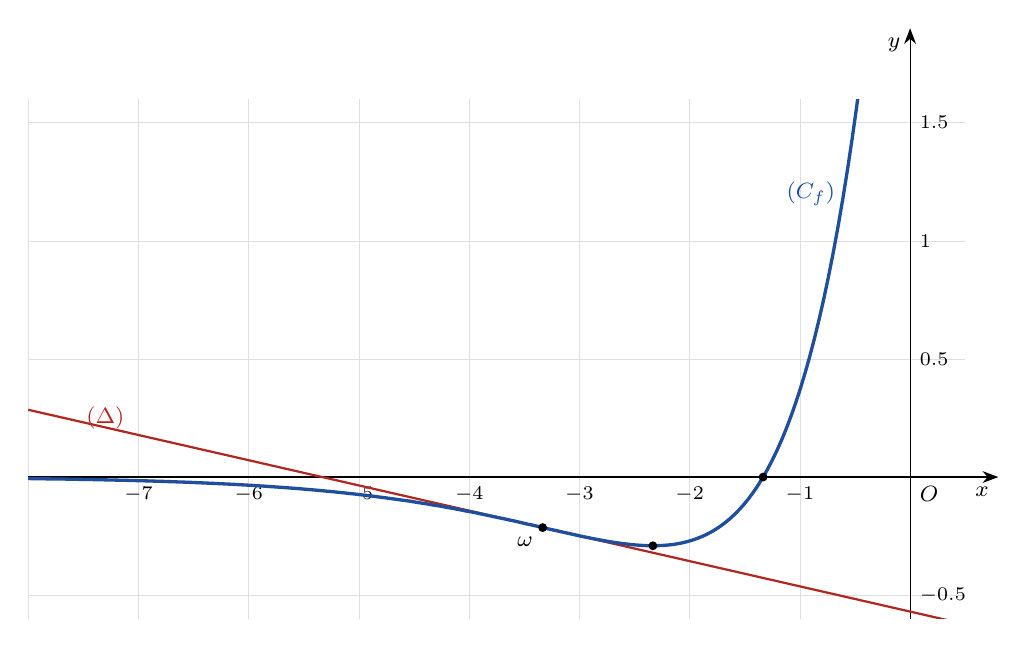
\begin{tikzpicture}[x=1.4cm,y=3cm,font=\footnotesize]
 \draw[gray!25,very thin,xstep=1,ystep=0.5] (-8,-0.6) grid (0.5,1.6);
 \draw[-{Stealth[length=2mm]}] (-8,0)--(0.8,0) node[below left]{$x$};
 \draw[-{Stealth[length=2mm]}] (0,-0.6)--(0,1.9) node[below left]{$y$};
 \node[below right] at (0,0){$O$};
 \foreach \t in {-7,-6,-5,-4,-3,-2,-1} \node[below,font=\scriptsize] at (\t,0){$\t$};
 \foreach \t in {-0.5,0.5,1,1.5} \node[right,font=\scriptsize] at (0,\t){$\t$};
 \begin{scope}\clip (-8,-0.6) rectangle (0.5,1.6);
 \draw[cThm,thick,domain=-8:0.5] plot(\x,{-exp(-10/3)*(3*\x+16)});
 \draw[cDef,very thick,domain=-8:0.5,samples=200] plot(\x,{(3*\x+4)*exp(\x)});
 \end{scope}
 \fill (-3.3333,-0.2140) circle (1.6pt) node[below left]{$\omega$} (-2.3333,-0.2909) circle (1.6pt) (-1.3333,0) circle (1.6pt);
 \node[cThm] at (-7.3,0.25){$(\Delta)$};
 \node[cDef] at (-0.9,1.2){$(C_f)$};
\end{tikzpicture}\end{LTR}\end{center}
\end{hal}

% ===================== بكالوريا 2010 -- الموضوع الأول =====================
\begin{tamrin}{بكالوريا 2010 -- الموضوع الأول -- رياضيات}
\textbf{I)} $g$ الدالة العددية المعرفة على $\R$ بـ: $g(x)=(3-x)e^{x}-3$.
\QQ{1} أدرس تغيّرات الدالة $g$.
\QQ{2} بيّن أن المعادلة $g(x)=0$ تقبل حلين مختلفين أحدهما معدوم والآخر $\alpha$ حيث $2{,}82<\alpha<2{,}83$.
\QQ{3} استنتج إشارة $g(x)$ حسب قيم $x$.

\textbf{II)} $f$ الدالة المعرفة على $\R$ بـ: $\begin{cases} f(x)=\dfrac{x^3}{e^{x}-1}\ ;\ x\neq0\\[4pt] f(0)=0\end{cases}$
و $(C_f)$ تمثيلها البياني في المستوي المنسوب إلى المعلم المتعامد والمتجانس $(O;\vec i,\vec j)$.
\QQ{1} بيّن أن الدالة $f$ تقبل الاشتقاق عند $x_0=0$. أكتب معادلة لـ $(T)$ مماس $(C_f)$ عند المبدأ $O$.
\QQ{2}
\begin{sq}
\qa بيّن أن $\lim\limits_{x\to+\infty}x^3e^{-x}=0$، ثم جد $\lim\limits_{x\to+\infty}f(x)$، وأحسب $\lim\limits_{x\to-\infty}f(x)$.
\qb بيّن أنه من أجل $x\neq0$ فإن: $f'(x)=\dfrac{x^2g(x)}{(e^{x}-1)^2}$.
\qc تحقق أن: $f(\alpha)=\alpha^2(3-\alpha)$، ثم عيّن حصرا له.
\qd أنشئ جدول تغيّرات $f$.
\end{sq}
\QQ{3}
\begin{sq}
\qa أحسب $f(x)+x^3$ واستنتج الوضعية النسبية لـ $(C_f)$ و $(C)$ منحنى الدالة $x\mapsto-x^3$.
\qb بيّن أن $\lim\limits_{x\to-\infty}\left[f(x)+x^3\right]=0$ وفسّر النتيجة هندسيا.
\end{sq}
\QQ{4} أنشئ في نفس المعلم المماس $(T)$ والمنحنيين $(C_f)$ و $(C)$.
\end{tamrin}

\begin{hal}
\textbf{الجزء الأول:}

\QQ{1} \textbf{النهايات:} $(3-x)e^{x}=3e^{x}-xe^{x}$ و $\lim\limits_{x\to-\infty}xe^{x}=0$، إذن \bx{\lim\limits_{x\to-\infty}g(x)=-3}.
$\lim\limits_{x\to+\infty}(3-x)=-\infty$ و $\lim\limits_{x\to+\infty}e^{x}=+\infty$، إذن \bx{\lim\limits_{x\to+\infty}g(x)=-\infty}.

\textbf{المشتقة:} $g'(x)=-e^{x}+(3-x)e^{x}=(2-x)e^{x}$، وإشارتها إشارة $(2-x)$. $g(2)=e^2-3\approx4{,}39$.
\begin{TAB}
\tkzTabInit[lgt=2,espcl=3.5]{$x$/1,$g'(x)$/1,$g(x)$/2}{$-\infty$,$2$,$+\infty$}
\tkzTabLine{,+,z,-,}
\tkzTabVar{-/$-3$,+/$e^2-3$,-/$-\infty$}
\end{TAB}
$g$ متزايدة تماما على $]{-}\infty;2]$ ومتناقصة تماما على $[2;+\infty[$.

\QQ{2} \begin{itemize}
\item على $]{-}\infty;2]$: $g$ مستمرة ومتزايدة تماما، و $g(0)=3-3=0$: إذن $0$ هو الحل الوحيد في هذا المجال.
\item على $[2;+\infty[$: $g$ مستمرة ومتناقصة تماما من $e^2-3>0$ إلى $-\infty$: حل وحيد $\alpha$. و $g(2{,}82)\approx0{,}020>0$ و $g(2{,}83)\approx-0{,}119<0$، إذن حسب مبرهنة القيم المتوسطة: \bx{2{,}82<\alpha<2{,}83}.
\end{itemize}

\QQ{3}
\begin{TAB}
\tkzTabInit[lgt=2,espcl=2.8]{$x$/1,$g(x)$/1}{$-\infty$,$0$,$\alpha$,$+\infty$}
\tkzTabLine{,-,z,+,z,-,}
\end{TAB}

\textbf{الجزء الثاني:}

\QQ{1} من أجل $x\neq0$:
\[\frac{f(x)-f(0)}{x-0}=\frac{x^2}{e^{x}-1}=x\times\frac{x}{e^{x}-1}=x\times\frac{1}{\;\dfrac{e^{x}-1}{x}\;}\]
و $\lim\limits_{x\to0}\dfrac{e^{x}-1}{x}=1$، إذن $\lim\limits_{x\to0}\dfrac{f(x)-f(0)}{x}=0\times1=0$:
\bxt{$f$ تقبل الاشتقاق عند $0$ و $f'(0)=0$}.
معادلة المماس: $y=f'(0)(x-0)+f(0)$، أي \bx{(T):\ y=0} (محور الفواصل).

\QQ{2}
\pa $x^3e^{-x}=27\left(\dfrac{x}{3}e^{-\frac x3}\right)^3=27\left(\dfrac{\frac x3}{e^{\frac x3}}\right)^3$، وبوضع $t=\dfrac x3\to+\infty$: $\lim\limits_{t\to+\infty}\dfrac{t}{e^{t}}=0$، إذن \bx{\lim\limits_{x\to+\infty}x^3e^{-x}=0}.

$f(x)=\dfrac{x^3}{e^{x}\left(1-e^{-x}\right)}=\dfrac{x^3e^{-x}}{1-e^{-x}}$، ومنه \bx{\lim\limits_{x\to+\infty}f(x)=\dfrac{0}{1-0}=0}.

عند $-\infty$: $\lim\limits_{x\to-\infty}x^3=-\infty$ و $\lim\limits_{x\to-\infty}(e^{x}-1)=-1$، إذن \bx{\lim\limits_{x\to-\infty}f(x)=+\infty}.

\pb من أجل $x\neq0$:
\[f'(x)=\frac{3x^2(e^{x}-1)-x^3e^{x}}{(e^{x}-1)^2}=\frac{x^2\left[3e^{x}-3-xe^{x}\right]}{(e^{x}-1)^2}=\frac{x^2\left[(3-x)e^{x}-3\right]}{(e^{x}-1)^2}=\bx{\frac{x^2g(x)}{(e^{x}-1)^2}}\]

\pc $g(\alpha)=0\iff(3-\alpha)e^{\alpha}=3\iff e^{\alpha}=\dfrac3{3-\alpha}$، ومنه $e^{\alpha}-1=\dfrac{3-3+\alpha}{3-\alpha}=\dfrac{\alpha}{3-\alpha}$، و:
\[f(\alpha)=\frac{\alpha^3}{\frac{\alpha}{3-\alpha}}=\bx{\alpha^2(3-\alpha)}\]
\textbf{الحصر:} نضع $u(x)=x^2(3-x)=3x^2-x^3$؛ $u'(x)=3x(2-x)<0$ على $[2{,}82;2{,}83]$، فـ $u$ متناقصة تماما عليه، ومنه:
\[u(2{,}83)<f(\alpha)<u(2{,}82)\quad\Longrightarrow\quad \bx{1{,}36<f(\alpha)<1{,}44}\]
(لأن $u(2{,}83)\approx1{,}3615$ و $u(2{,}82)\approx1{,}4314$).

\pd من أجل $x\neq0$: $x^2>0$ و $(e^{x}-1)^2>0$، إذن إشارة $f'(x)$ هي إشارة $g(x)$، و $f'(0)=0$:
\begin{TAB}
\tkzTabInit[lgt=2,espcl=2.8]{$x$/1,$f'(x)$/1,$f(x)$/2.2}{$-\infty$,$0$,$\alpha$,$+\infty$}
\tkzTabLine{,-,z,+,z,-,}
\tkzTabVar{+/$+\infty$,-/$0$,+/$f(\alpha)$,-/$0$}
\end{TAB}

\QQ{3}
\pa من أجل $x\neq0$:
\[f(x)+x^3=x^3\left(\frac{1}{e^{x}-1}+1\right)=\bx{\frac{x^3e^{x}}{e^{x}-1}}\]
$e^{x}>0$، و $x^3$ و $e^{x}-1$ لهما نفس الإشارة (كلاهما سالب لما $x<0$ وموجب لما $x>0$)، إذن $f(x)+x^3>0$ من أجل $x\neq0$، و $f(0)+0=0$:
\bxt{$(C_f)$ فوق $(C)$ على $\R^*$، ويتقاطعان في المبدأ $O$}.

\pb $\lim\limits_{x\to-\infty}x^3e^{x}=0$ (تزايد مقارن) و $\lim\limits_{x\to-\infty}(e^{x}-1)=-1$، إذن \bx{\lim\limits_{x\to-\infty}\left[f(x)+x^3\right]=0}.
\textbf{التفسير الهندسي:} المنحنيان $(C_f)$ و $(C)$ متقاربان (متجاوران) عند $-\infty$.

\QQ{4} \textbf{الرسم:} $f(-1)\approx1{,}58$، $f(1)\approx0{,}58$، $f(2)\approx1{,}25$، $f(\alpha)\approx1{,}42$، $f(5)\approx0{,}85$.
\begin{GR}{-2.5}{8.5}{-1.5}{5}{1.2}
 \Ticks{-2,-1,1,2,3,4,5,6,7,8}{-1,1,2,3,4}
 \draw[cThm,thick] (-2.5,0)--(8.5,0); \node[cThm,above] at (7.6,0){$(T)$};
 \draw[cRem,thick,domain=-1.72:1.2,samples=100] plot(\x,{-\x*\x*\x});
 \draw[cDef,very thick,domain=-2.5:-0.01,samples=120] plot(\x,{\x*\x*\x/(exp(\x)-1)});
 \draw[cDef,very thick,domain=0.01:8.5,samples=150] plot(\x,{\x*\x*\x/(exp(\x)-1)});
 \draw[cDef,very thick] (-0.01,0)--(0.01,0);
 \fill (0,0) circle (1.6pt) (2.8214,1.4214) circle (1.6pt);
 \draw[dashed,gray] (2.8214,0)--(2.8214,1.4214);
 \node[below] at (2.8214,0){$\alpha$};
 \node[cDef] at (-1.6,4.4){$(C_f)$};
 \node[cRem] at (-0.6,1.6){$(C)$};
 \node[cDef] at (5,1.25){$(C_f)$};
\end{GR}
\end{hal}

% ===================== بكالوريا 2008 -- الموضوع الثاني =====================
\begin{tamrin}{بكالوريا 2008 -- الموضوع الثاني -- رياضيات}
\textbf{I)} $f$ الدالة العددية المعرفة على $\R$ بـ: $f(x)=x-1+\dfrac{4}{e^{x}+1}$،
وليكن $(C_f)$ تمثيلها البياني في المستوي المنسوب إلى المعلم المتعامد والمتجانس $(O;\vec i,\vec j)$.
\QQ{1} أدرس تغيّرات الدالة $f$.
\QQ{2}
\begin{sq}
\qa بيّن أن $(C_f)$ يقبل نقطة انعطاف $w$، وأكتب معادلة مماس $(C_f)$ عند $w$.
\qb أثبت أن $w$ مركز تناظر للمنحنى $(C_f)$.
\end{sq}
\QQ{3}
\begin{sq}
\qa أحسب $\lim\limits_{x\to+\infty}\left[f(x)-(x-1)\right]$ و $\lim\limits_{x\to-\infty}\left[f(x)-(x+3)\right]$.
\qb استنتج أن $(C_f)$ يقبل مقاربين يطلب إعطاء معادلة لكل منهما.
\end{sq}
\QQ{4}
\begin{sq}
\qa بيّن أن $(C_f)$ يقطع حامل محور الفواصل في نقطة وحيدة فاصلتها $x_0$ حيث $x_0\in]-2{,}77;-2{,}76[$.
\qb أحسب $f(1)$ و $f(-1)$ (تدوّر النتائج إلى $10^{-2}$)، ثم أرسم $(C_f)$ ومستقيميه المقاربين.
\end{sq}

\textbf{II)} $g$ الدالة العددية المعرفة على $\R$ بـ: $g(x)=-x+3-\dfrac{4}{e^{x}+1}$، وليكن $(C_g)$ تمثيلها البياني.
\QQ{1}
\begin{sq}
\qa بيّن أنه من أجل كل عدد حقيقي $x$ فإن: $g(x)=f(-x)$.
\qb استنتج أنه يوجد تحويل نقطي بسيط يحوّل $(C_f)$ إلى $(C_g)$.
\end{sq}
\QQ{2} أنشئ $(C_g)$ في نفس المعلم السابق (دون دراسة $g$).
\end{tamrin}

\begin{hal}
\textbf{الجزء الأول:}

\QQ{1} \textbf{النهايات:} $\lim\limits_{x\to+\infty}e^{x}=+\infty$ إذن $\lim\limits_{x\to+\infty}\dfrac4{e^{x}+1}=0$، ومنه \bx{\lim\limits_{x\to+\infty}f(x)=+\infty}.
$\lim\limits_{x\to-\infty}e^{x}=0$ إذن $\lim\limits_{x\to-\infty}\dfrac4{e^{x}+1}=4$، ومنه \bx{\lim\limits_{x\to-\infty}f(x)=-\infty}.

\textbf{المشتقة:} $f$ قابلة للاشتقاق على $\R$، و:
\[f'(x)=1-\frac{4e^{x}}{(e^{x}+1)^2}=\frac{e^{2x}+2e^{x}+1-4e^{x}}{(e^{x}+1)^2}=\bx{\frac{(e^{x}-1)^2}{(e^{x}+1)^2}}\]
إذن $f'(x)\geqslant0$، وتنعدم فقط عند $x=0$ (لأن $e^{x}=1\iff x=0$): $f$ متزايدة تماما على $\R$. $f(0)=-1+2=1$.
\begin{TAB}
\tkzTabInit[lgt=2,espcl=3.5]{$x$/1,$f'(x)$/1,$f(x)$/2}{$-\infty$,$0$,$+\infty$}
\tkzTabLine{,+,z,+,}
\tkzTabVar{-/$-\infty$,R/,+/$+\infty$}
\end{TAB}

\QQ{2}
\pa نضع $t=e^{x}$؛ $f'(x)=\left(\dfrac{t-1}{t+1}\right)^2$، و $\left(\dfrac{t-1}{t+1}\right)'=\dfrac{2t}{(t+1)^2}$ (بالنسبة إلى $x$: $t'=t$)، ومنه:
\[f''(x)=2\cdot\frac{e^{x}-1}{e^{x}+1}\cdot\frac{2e^{x}}{(e^{x}+1)^2}=\frac{4e^{x}(e^{x}-1)}{(e^{x}+1)^3}\]
إشارة $f''(x)$ هي إشارة $e^{x}-1$: سالبة على $]{-}\infty;0[$ وموجبة على $]0;+\infty[$؛ $f''$ تنعدم عند $0$ مغيّرة إشارتها، إذن \bxt{$w(0;1)$ نقطة انعطاف للمنحنى $(C_f)$}.
المماس عند $w$: $y=f'(0)(x-0)+f(0)=0\cdot x+1$، أي \bx{y=1}.

\pb من أجل كل $x\in\R$: $-x\in\R$، و:
\[f(-x)=-x-1+\frac{4}{e^{-x}+1}=-x-1+\frac{4e^{x}}{1+e^{x}}\]
\[f(x)+f(-x)=-2+\frac{4+4e^{x}}{e^{x}+1}=-2+4=2=2\times1\]
إذن $f(2\times0-x)+f(x)=2\times1$: \bxt{$w(0;1)$ مركز تناظر للمنحنى $(C_f)$}.

\QQ{3}
\pa $\lim\limits_{x\to+\infty}\left[f(x)-(x-1)\right]=\lim\limits_{x\to+\infty}\dfrac4{e^{x}+1}=\bx{0}$.

$f(x)-(x+3)=-4+\dfrac4{e^{x}+1}$، إذن $\lim\limits_{x\to-\infty}\left[f(x)-(x+3)\right]=-4+\dfrac4{0+1}=\bx{0}$.

\pb إذن $(C_f)$ يقبل مستقيمين مقاربين مائلين: \bx{y=x-1} عند $+\infty$، و \bx{y=x+3} عند $-\infty$.

\QQ{4}
\pa $f$ مستمرة ومتزايدة تماما على $\R$ وتأخذ قيمها في $]{-}\infty;+\infty[$، إذن المعادلة $f(x)=0$ تقبل حلا وحيدا $x_0$.
$f(-2{,}77)\approx-0{,}006<0$ و $f(-2{,}76)\approx0{,}002>0$، إذن حسب مبرهنة القيم المتوسطة: \bx{x_0\in]-2{,}77;-2{,}76[}.

\pb $f(1)=\dfrac{4}{e+1}\approx\bx{1{,}08}$ \ و \ $f(-1)=-2+\dfrac{4}{e^{-1}+1}\approx\bx{0{,}92}$ (ونلاحظ $f(1)+f(-1)=2$).
\textbf{الرسم:} أنظر الشكل بعد الجزء الثاني (المنحنى $(C_f)$ بالأزرق).

\textbf{الجزء الثاني:}

\QQ{1}
\pa من أجل كل $x\in\R$:
\[f(-x)=-x-1+\frac{4e^{x}}{e^{x}+1}=-x-1+\frac{4(e^{x}+1)-4}{e^{x}+1}=-x-1+4-\frac{4}{e^{x}+1}=-x+3-\frac4{e^{x}+1}\]
إذن \bx{g(x)=f(-x)}.

\pb $M(x;y)\in(C_g)\iff y=f(-x)\iff M'(-x;y)\in(C_f)$، إذن:
\bxt{$(C_g)$ هو نظير $(C_f)$ بالنسبة إلى محور التراتيب}.

\QQ{2} \textbf{الرسم:} مقاربا $(C_g)$ هما نظيرا مقاربي $(C_f)$: $y=-x-1$ عند $-\infty$ و $y=-x+3$ عند $+\infty$، و $(C_g)$ يقطع محور الفواصل في $-x_0\approx2{,}76$.
\begin{GR}{-5}{5}{-4}{5}{0.95}
 \Ticks{-4,-3,-2,-1,1,2,3,4}{-3,-2,-1,1,2,3,4}
 \draw[cThm,dashed,thick,domain=-5:5] plot(\x,{\x-1});
 \draw[cThm,dashed,thick,domain=-5:5] plot(\x,{\x+3});
 \draw[cRem,dashed,thin,domain=-5:5] plot(\x,{-\x-1});
 \draw[cRem,dashed,thin,domain=-5:5] plot(\x,{-\x+3});
 \draw[gray,thin] (-5,1)--(5,1);
 \draw[cDef,very thick,domain=-5:5,samples=150] plot(\x,{\x-1+4/(exp(\x)+1)});
 \draw[cRem,very thick,domain=-5:5,samples=150] plot(\x,{-\x+3-4/(exp(\x)+1)});
 \fill (0,1) circle (1.6pt) node[above left]{$w$} (-2.7625,0) circle (1.6pt) (2.7625,0) circle (1.6pt) (1,1.0758) circle (1.4pt) (-1,0.9242) circle (1.4pt);
 \node[cDef] at (3.9,2.1){$(C_f)$};
 \node[cRem] at (-3.9,2.1){$(C_g)$};
 \node[cThm,font=\scriptsize] at (4.3,3.75){$y=x-1$};
 \node[cThm,font=\scriptsize] at (-1.6,2.1){$y=x+3$};
\end{GR}
\end{hal}
\end{document}
